% ============================================================
%  TTM4100 KTN -- Complete Study Guide
%  All chapters combined for Overleaf
%  NTNU, Spring 2026
% ============================================================

\documentclass[11pt,a4paper]{article}

% ── Encoding & fonts ──────────────────────────────────────────────────────────
\usepackage[utf8]{inputenc}
\usepackage[T1]{fontenc}
\usepackage{lmodern}

% ── Page geometry ─────────────────────────────────────────────────────────────
\usepackage[top=2.5cm, bottom=2.5cm, left=2.5cm, right=2.5cm]{geometry}

% ── Core math & graphics ──────────────────────────────────────────────────────
\usepackage{graphicx}
\usepackage{float}
\graphicspath{{Bilder/}}
\usepackage{amsmath,amssymb}

% ── TikZ ──────────────────────────────────────────────────────────────────────
\usepackage{tikz}
\usetikzlibrary{shapes,arrows.meta,positioning,calc,decorations.pathreplacing,fit}

% ── Colours ───────────────────────────────────────────────────────────────────
\usepackage{xcolor}
\definecolor{ntnu}{RGB}{0,80,158}
\definecolor{ntnublue}{RGB}{0,80,158}
\definecolor{ntnugold}{RGB}{241,174,35}
\definecolor{darkblue}{RGB}{0,0,139}
\definecolor{lightblue}{RGB}{220,235,255}
\definecolor{keyblue}{RGB}{220,235,250}
\definecolor{keyborder}{RGB}{30,100,200}
\definecolor{lightgreen}{RGB}{220,255,220}
\definecolor{formulabg}{RGB}{225,245,225}
\definecolor{formulaborder}{RGB}{0,140,0}
\definecolor{lightyellow}{RGB}{255,255,220}
\definecolor{warnbg}{RGB}{255,248,220}
\definecolor{warnborder}{RGB}{200,140,0}
\definecolor{lightred}{RGB}{255,220,220}
\definecolor{codebg}{RGB}{245,245,245}
\definecolor{ntnulight}{RGB}{230,240,255}
\definecolor{warnyellow}{RGB}{255,200,0}
\definecolor{formulagreen}{RGB}{0,120,60}
\definecolor{examred}{RGB}{180,0,0}
\definecolor{exambg}{RGB}{255,230,230}
\definecolor{examborder}{RGB}{180,0,0}
\definecolor{tocline}{RGB}{0,80,158}
\definecolor{chapterbg}{RGB}{0,80,158}

% ── Hyperlinks ────────────────────────────────────────────────────────────────
\usepackage{hyperref}
\hypersetup{
  colorlinks=true,
  linkcolor=ntnu,
  urlcolor=ntnu!80!black,
  citecolor=ntnu,
  pdftitle={TTM4100 KTN -- Complete Study Guide},
  pdfauthor={Markus Selander, NTNU Spring 2026},
}

% ── Lists & tables ────────────────────────────────────────────────────────────
\usepackage{enumitem}
\usepackage{booktabs}
\usepackage{longtable}
\usepackage{array}
\usepackage{multicol}

% ── Code listings ─────────────────────────────────────────────────────────────
\usepackage{listings}
\lstset{
  backgroundcolor=\color{codebg},
  basicstyle=\ttfamily\small,
  breaklines=true,
  frame=single,
  rulecolor=\color{ntnu!40},
}

% ── Coloured boxes ────────────────────────────────────────────────────────────
\usepackage{tcolorbox}
\tcbuselibrary{skins,breakable}

% Named environments (used by chapters 1-7 as \begin{keybox}[Title])
\newtcolorbox{keybox}[1][]{colback=keyblue,colframe=keyborder,title=#1,fonttitle=\bfseries,breakable}
\newtcolorbox{warnbox}[1][]{colback=warnbg,colframe=warnborder,title=#1,fonttitle=\bfseries,breakable}
\newtcolorbox{formulabox}[1][]{colback=formulabg,colframe=formulaborder,title=#1,fonttitle=\bfseries,breakable}
\newtcolorbox{exambox}[1][]{colback=lightred,colframe=red!70!black,title=#1,fonttitle=\bfseries,breakable}
\newtcolorbox{imagebox}[1][]{colback=yellow!8,colframe=orange!70!black,title={\small\textbf{IMAGE PLACEHOLDER} -- #1},fonttitle=\color{orange!70!black},breakable,left=4pt,right=4pt,top=2pt,bottom=2pt}

% Named styles (used by chapters 8-9 as \begin{tcolorbox}[keybox, title=...])
\tcbset{
  keybox/.style={colback=keyblue, colframe=keyborder,
    fonttitle=\bfseries, breakable},
  warnbox/.style={colback=warnbg, colframe=warnborder,
    fonttitle=\bfseries, breakable},
  formulabox/.style={colback=formulabg, colframe=formulaborder,
    fonttitle=\bfseries, breakable},
  exambox/.style={colback=exambg, colframe=examborder,
    fonttitle=\bfseries, breakable},
}

% ── Section titles ────────────────────────────────────────────────────────────
\usepackage{titlesec}
\titleformat{\section}
  {\large\bfseries\color{ntnublue}}
  {\color{ntnublue}\thesection}{0.8em}{}[\color{ntnublue}\titlerule]
\titleformat{\subsection}
  {\normalsize\bfseries\color{ntnublue!80}}
  {\thesubsection}{0.6em}{}
\titleformat{\subsubsection}
  {\small\bfseries\color{ntnublue!60}}
  {\thesubsubsection}{0.5em}{}

% ── Table of contents styling ────────────────────────────────────────────────
\usepackage{tocloft}

% TOC title
\renewcommand{\cfttoctitlefont}{\Huge\bfseries\color{ntnublue}}
\renewcommand{\cftaftertoctitle}{%
  \par\noindent\color{ntnublue}\rule{\linewidth}{2pt}\par\vspace{4pt}
}
\setlength{\cftbeforetoctitleskip}{0pt}
\setlength{\cftaftertoctitleskip}{12pt}

% Section entries
\renewcommand{\cftsecfont}{\bfseries\color{ntnublue}}
\renewcommand{\cftsecpagefont}{\bfseries\color{ntnublue}}
\renewcommand{\cftsecleader}{\color{ntnublue!40}\cftdotfill{\cftdotsep}}
\setlength{\cftsecindent}{0pt}
\setlength{\cftsecnumwidth}{2.2em}
\setlength{\cftbeforesecskip}{4pt}

% Subsection entries
\renewcommand{\cftsubsecfont}{\color{black!80}}
\renewcommand{\cftsubsecpagefont}{\color{black!60}}
\renewcommand{\cftsubsecleader}{\color{black!25}\cftdotfill{\cftdotsep}}
\setlength{\cftsubsecindent}{2.2em}
\setlength{\cftsubsecnumwidth}{2.8em}
\setlength{\cftbeforesubsecskip}{1pt}

% Subsubsection entries
\renewcommand{\cftsubsubsecfont}{\small\color{black!60}}
\renewcommand{\cftsubsubsecpagefont}{\small\color{black!50}}
\setlength{\cftsubsubsecindent}{5em}
\setlength{\cftbeforesubsubsecskip}{0pt}

% TOC depth
\setcounter{tocdepth}{2}
\setcounter{secnumdepth}{3}

% ── Headers & footers ─────────────────────────────────────────────────────────
\usepackage{fancyhdr}
\pagestyle{fancy}
\fancyhf{}
\fancyhead[L]{\textcolor{ntnublue}{\textbf{TTM4100 -- KTN}}}
\fancyhead[C]{\textcolor{black!60}{\small\leftmark}}
\fancyhead[R]{\textcolor{ntnugold}{\textbf{NTNU}}}
\fancyfoot[L]{\textcolor{black!40}{\small Study Notes -- Spring 2026}}
\fancyfoot[C]{\textcolor{ntnublue}{\thepage}}
\fancyfoot[R]{\textcolor{black!40}{\small Markus Selander}}
\renewcommand{\headrulewidth}{0.4pt}
\renewcommand{\footrulewidth}{0.4pt}
\renewcommand{\headrule}{\color{ntnublue}\hrule width\headwidth height\headrulewidth}
\renewcommand{\footrule}{\color{ntnublue!40}\hrule width\headwidth height\footrulewidth}

% ── Chapter divider command ───────────────────────────────────────────────────
\newcommand{\chapterdivider}[2]{%
  \newpage
  \thispagestyle{empty}
  \vspace*{4cm}
  \begin{tikzpicture}[remember picture, overlay]
    \fill[ntnublue] (current page.north west) rectangle
      ([yshift=-3mm]current page.north east);
    \fill[ntnugold] ([yshift=-3mm]current page.north west) rectangle
      ([yshift=-6mm]current page.north east);
  \end{tikzpicture}
  \begin{center}
    \begin{tcolorbox}[
      colback=ntnublue,
      colframe=ntnugold,
      coltext=white,
      boxrule=2pt,
      arc=4pt,
      width=0.85\textwidth,
      halign=center,
    ]
      {\large\bfseries\color{ntnugold} TTM4100 -- KTN}\\[6pt]
      {\Huge\bfseries\color{white} #2}\\[6pt]
      {\normalsize\color{white!80} Computer Networking: A Top-Down Approach, 8th ed.\\
       Kurose \& Ross \quad -- \quad NTNU Spring 2026}
    \end{tcolorbox}
  \end{center}
  \vspace{1cm}
  \markboth{#2}{#2}
  \addcontentsline{toc}{section}{\protect\numberline{}{\color{ntnublue}\bfseries #2}}
  \newpage
}

% ── Figure image commands ─────────────────────────────────────────────────────
\newcommand{\figureimg}[2][0.95\linewidth]{%
  \begin{figure}[H]
    \centering
    \includegraphics[width=#1]{#2}
  \end{figure}%
}

\newcommand{\figureimgpair}[2]{%
  \begin{figure}[H]
    \centering
    \includegraphics[width=0.48\linewidth]{#1}\hfill
    \includegraphics[width=0.48\linewidth]{#2}
  \end{figure}%
}

\newcommand{\figureimgtriple}[3]{%
  \begin{figure}[H]
    \centering
    \includegraphics[width=0.32\linewidth]{#1}\hfill
    \includegraphics[width=0.32\linewidth]{#2}\hfill
    \includegraphics[width=0.32\linewidth]{#3}
  \end{figure}%
}

% ============================================================
\begin{document}

% ── Cover page ────────────────────────────────────────────────────────────────
\begin{titlepage}
  \begin{tikzpicture}[remember picture, overlay]
    \fill[ntnublue] (current page.north west) rectangle
      ([yshift=-8cm]current page.north east);
    \fill[ntnugold] ([yshift=-8cm]current page.north west) rectangle
      ([yshift=-8.5cm]current page.north east);
  \end{tikzpicture}

  \vspace*{2cm}
  \begin{center}
    {\color{white}\fontsize{16}{20}\selectfont\bfseries TTM4100 -- Communication, Services and Networks}\\[0.5em]
    {\color{white!80}\large NTNU -- Norwegian University of Science and Technology}
  \end{center}

  \vspace{3.5cm}

  \begin{center}
    {\fontsize{40}{48}\selectfont\bfseries\color{ntnublue} Study Guide}\\[1em]
    {\Large\color{black!70} Chapters 1 -- 9}\\[2em]
    \color{ntnublue}\rule{0.6\textwidth}{1.5pt}\\[2em]
    {\large\color{black!60}
      \textit{Computer Networking: A Top-Down Approach}, 8th ed.\\[0.3em]
      Kurose \& Ross
    }\\[3em]
    {\normalsize\color{black!50}
      Markus Selander\\[0.2em]
      Spring 2026
    }
  \end{center}
\end{titlepage}

% ── Table of contents ─────────────────────────────────────────────────────────
\newpage
\thispagestyle{fancy}
{
  \hypersetup{linkcolor=ntnublue}
  \tableofcontents
}
\newpage

% ============================================================
%  CHAPTER 1
% ============================================================
\chapterdivider{1}{Chapter 1: Introduction}
\section{Hva er Internett?}
%=============================================================================

Internett kan beskrives fra to perspektiver: \textbf{``nuts and bolts''} (komponentene) og \textbf{``service''} (tjenestene).

\subsection{``Nuts and Bolts'' -- Komponentperspektivet}

\begin{keybox}[Internett er et ``network of networks'']
Internett best\aa r av milliarder tilkoblede enheter som kommuniserer via \textbf{pakkesvitsjer} (rutere og svitsjer) over \textbf{kommunikasjonslinker} (fiber, kobber, radio, satellitt).
\end{keybox}

\begin{center}
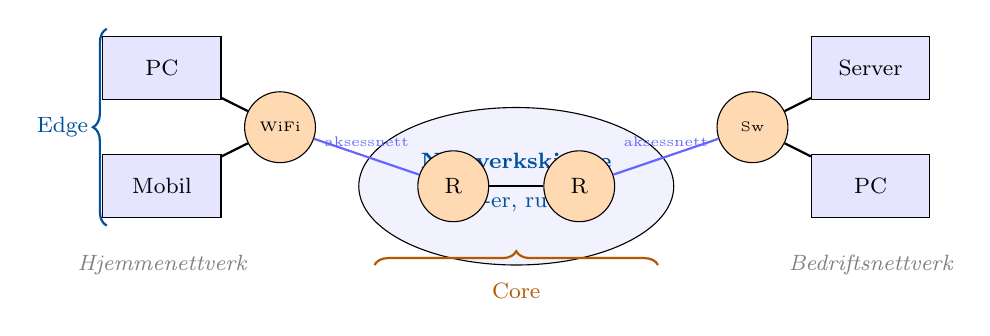
\begin{tikzpicture}[
    host/.style={rectangle, draw, fill=blue!10, minimum width=1.5cm, minimum height=0.8cm, font=\footnotesize},
    router/.style={circle, draw, fill=orange!30, minimum size=0.9cm, font=\footnotesize},
    cloud/.style={ellipse, draw, fill=blue!5, minimum width=4cm, minimum height=2cm},
    link/.style={thick, -},
    >=Stealth
]
    % ISP Cloud
    \node[cloud] (isp) at (0,0) {};
    \node[font=\footnotesize\bfseries, text=ntnu] at (0,0.3) {Nettverkskjerne};
    \node[font=\footnotesize, text=ntnu] at (0,-0.2) {(ISP-er, rutere)};

    % Routers inside
    \node[router] (r1) at (-0.8,0) {R};
    \node[router] (r2) at (0.8,0) {R};
    \draw[link] (r1) -- (r2);

    % Home network
    \node[host] (pc1) at (-4.5, 1.5) {PC};
    \node[host] (phone) at (-4.5, 0) {Mobil};
    \node[router] (hr) at (-3, 0.75) {\tiny WiFi};
    \draw[link] (pc1) -- (hr);
    \draw[link] (phone) -- (hr);
    \draw[link, blue!60, thick] (hr) -- (r1) node[midway, above, font=\tiny] {aksessnett};

    % Enterprise
    \node[host] (srv) at (4.5, 1.5) {Server};
    \node[host] (ws) at (4.5, 0) {PC};
    \node[router] (er) at (3, 0.75) {\tiny Sw};
    \draw[link] (srv) -- (er);
    \draw[link] (ws) -- (er);
    \draw[link, blue!60, thick] (er) -- (r2) node[midway, above, font=\tiny] {aksessnett};

    % Labels
    \node[font=\footnotesize\itshape, text=gray] at (-4.5, -1) {Hjemmenettverk};
    \node[font=\footnotesize\itshape, text=gray] at (4.5, -1) {Bedriftsnettverk};

    % Annotations
    \draw[decorate, decoration={brace,amplitude=5pt}, thick, ntnu] (-5.2,-0.5) -- (-5.2,2) node[midway, left, font=\footnotesize, text=ntnu, xshift=-3pt] {Edge};
    \draw[decorate, decoration={brace,amplitude=5pt}, thick, orange!70!black] (-1.8,-1) -- (1.8,-1) node[midway, below, font=\footnotesize, text=orange!70!black, yshift=-3pt] {Core};
\end{tikzpicture}
\end{center}

\textbf{Viktige komponenter:}
\begin{itemize}[noitemsep]
    \item \textbf{Hosts / endesystemer} -- enheter som kj\o rer nettverksapplikasjoner (PC-er, mobiler, servere, IoT)
    \item \textbf{Pakkesvitsjer} -- videresender pakker: \emph{rutere} (nettverkslaget) og \emph{svitsjer} (linklaget)
    \item \textbf{Kommunikasjonslinker} -- fiber, kobber, radio, satellitt. Overf\o ringsrate = \emph{b\aa ndbredde}
    \item \textbf{Nettverk} -- samling av enheter, rutere og linker styrt av en organisasjon
    \item \textbf{ISP} (Internet Service Provider) -- gir tilgang til Internett
\end{itemize}

\begin{keybox}[Internettstandarder]
\begin{itemize}[noitemsep]
    \item \textbf{RFC} (Request for Comments) -- dokumenter som beskriver standardene
    \item \textbf{IETF} (Internet Engineering Task Force) -- utvikler standardene
\end{itemize}
\end{keybox}

\subsection{``Service'' -- Tjenesteperspektivet}

Internett er en \textbf{infrastruktur som leverer tjenester til applikasjoner}: web, video, e-post, spill, e-handel, sosiale medier, IoT, etc.

Internett tilbyr et \textbf{programmeringsgrensesnitt} (socket API) til distribuerte applikasjoner -- ``hooks'' som lar apper koble seg til og bruke transporttjenester.

%=============================================================================
\section{Hva er en protokoll?}
%=============================================================================

\begin{keybox}[Definisjon: Protokoll]
En \textbf{protokoll} definerer \textbf{formatet}, \textbf{rekkef\o lgen} av meldinger som sendes og mottas mellom nettverksenheter, og \textbf{handlingene} som utf\o res n\aa r meldinger sendes eller mottas.
\end{keybox}

\begin{center}
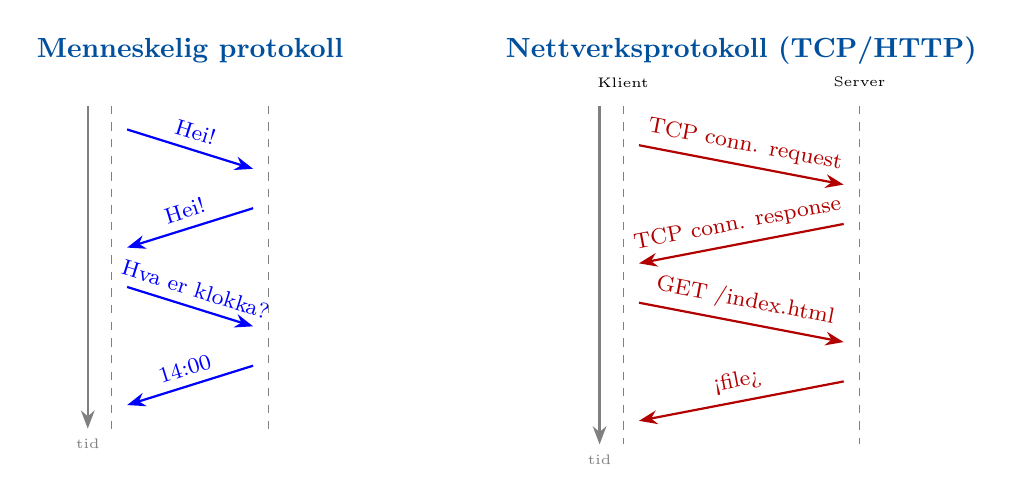
\begin{tikzpicture}[>=Stealth, font=\footnotesize]
    % Human protocol
    \node[font=\bfseries, text=ntnu] at (-3.5, 4.5) {Menneskelig protokoll};
    \node[inner sep=0pt] (p1) at (-4.5, 4) {};
    \node[inner sep=0pt] (p2) at (-2.5, 4) {};

    \draw[->, thick, blue] (-4.3, 3.5) -- (-2.7, 3.0) node[midway, above, sloped] {Hei!};
    \draw[->, thick, blue] (-2.7, 2.5) -- (-4.3, 2.0) node[midway, above, sloped] {Hei!};
    \draw[->, thick, blue] (-4.3, 1.5) -- (-2.7, 1.0) node[midway, above, sloped] {Hva er klokka?};
    \draw[->, thick, blue] (-2.7, 0.5) -- (-4.3, 0.0) node[midway, above, sloped] {14:00};

    % Dashed line
    \draw[dashed, gray] (-4.5, 3.8) -- (-4.5, -0.3);
    \draw[dashed, gray] (-2.5, 3.8) -- (-2.5, -0.3);

    % Network protocol
    \node[font=\bfseries, text=ntnu] at (3.5, 4.5) {Nettverksprotokoll (TCP/HTTP)};
    \node[inner sep=0pt] (c) at (2, 4) {};
    \node[inner sep=0pt] (s) at (5, 4) {};

    \node[font=\tiny] at (2, 4.1) {Klient};
    \node[font=\tiny] at (5, 4.1) {Server};

    \draw[->, thick, red!70!black] (2.2, 3.3) -- (4.8, 2.8) node[midway, above, sloped] {TCP conn. request};
    \draw[->, thick, red!70!black] (4.8, 2.3) -- (2.2, 1.8) node[midway, above, sloped] {TCP conn. response};
    \draw[->, thick, red!70!black] (2.2, 1.3) -- (4.8, 0.8) node[midway, above, sloped] {GET /index.html};
    \draw[->, thick, red!70!black] (4.8, 0.3) -- (2.2, -0.2) node[midway, above, sloped] {<file>};

    \draw[dashed, gray] (2, 3.8) -- (2, -0.5);
    \draw[dashed, gray] (5, 3.8) -- (5, -0.5);

    % Time arrows
    \draw[->, gray, thick] (-4.8, 3.8) -- (-4.8, -0.3) node[below, font=\tiny] {tid};
    \draw[->, gray, thick] (1.7, 3.8) -- (1.7, -0.5) node[below, font=\tiny] {tid};
\end{tikzpicture}
\end{center}

All kommunikasjonsaktivitet p\aa\ Internett er styrt av protokoller.

%=============================================================================
\section{Nettverkets ytterkant (Network Edge)}
%=============================================================================

\subsection{Hosts: Klienter og servere}
\begin{itemize}[noitemsep]
    \item \textbf{Hosts} (endesystemer) sitter i nettverkets ``edge''
    \item To typer: \textbf{klienter} (foresp\o r tjenester) og \textbf{servere} (tilbyr tjenester)
    \item Servere er ofte i \textbf{datasentre}
\end{itemize}

\subsection{Aksessnettverk (Access Networks)}

Aksessnettverket kobler endesystemer til den f\o rste ruteren (``edge router'').

\bigskip
\begin{center}
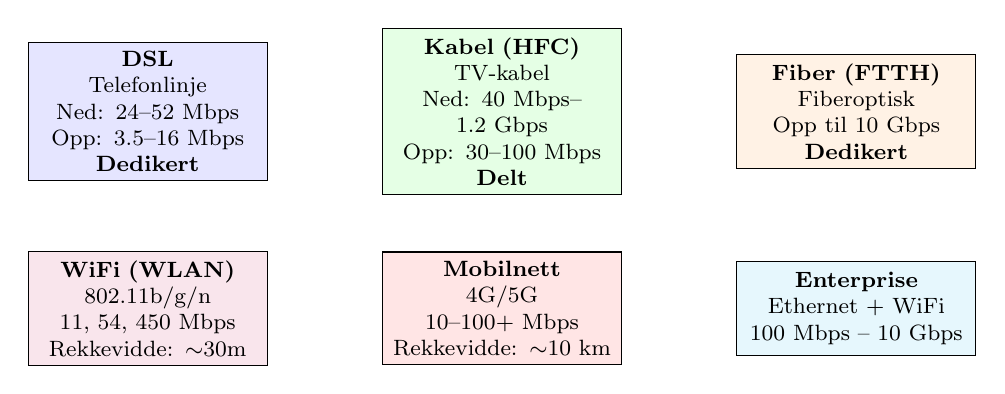
\begin{tikzpicture}[
    box/.style={rectangle, draw, fill=#1, minimum width=3cm, minimum height=1.2cm, text width=2.8cm, align=center, font=\footnotesize},
    >=Stealth
]
    \node[box=blue!10] (dsl) at (0,0) {\textbf{DSL}\\Telefonlinje\\Ned: 24--52 Mbps\\Opp: 3.5--16 Mbps\\\textbf{Dedikert}};
    \node[box=green!10] (cable) at (4.5,0) {\textbf{Kabel (HFC)}\\TV-kabel\\Ned: 40 Mbps--1.2 Gbps\\Opp: 30--100 Mbps\\\textbf{Delt}};
    \node[box=orange!10] (fiber) at (9,0) {\textbf{Fiber (FTTH)}\\Fiberoptisk\\Opp til 10 Gbps\\\textbf{Dedikert}};

    \node[box=purple!10] (wifi) at (0,-2.5) {\textbf{WiFi (WLAN)}\\802.11b/g/n\\11, 54, 450 Mbps\\Rekkevidde: $\sim$30m};
    \node[box=red!10] (cell) at (4.5,-2.5) {\textbf{Mobilnett}\\4G/5G\\10--100+ Mbps\\Rekkevidde: $\sim$10 km};
    \node[box=cyan!10] (ent) at (9,-2.5) {\textbf{Enterprise}\\Ethernet + WiFi\\100 Mbps -- 10 Gbps};
\end{tikzpicture}
\end{center}

\begin{warnbox}[Delt vs. dedikert aksess]
\begin{itemize}[noitemsep]
    \item \textbf{DSL}: Dedikert linje til sentralen (DSLAM) -- ingen deling med naboer
    \item \textbf{Kabel}: Delt medium -- alle i nabolaget deler b\aa ndbredden til ``cable headend''
\end{itemize}
\end{warnbox}

\subsection{Hjemmenettverk}

\begin{center}
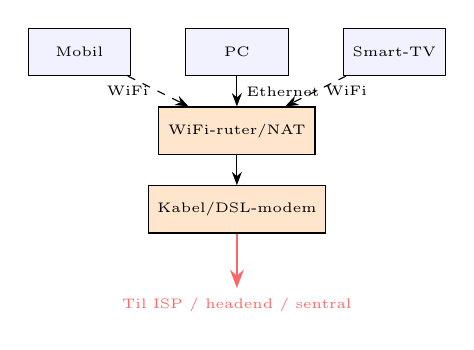
\begin{tikzpicture}[
    device/.style={rectangle, draw, fill=blue!5, minimum width=1.3cm, minimum height=0.6cm, font=\tiny},
    router/.style={rectangle, draw, fill=orange!20, minimum width=1.5cm, minimum height=0.6cm, font=\tiny},
    >=Stealth
]
    % Devices
    \node[device] (mob) at (-2, 1) {Mobil};
    \node[device] (pc) at (0, 1) {PC};
    \node[device] (tv) at (2, 1) {Smart-TV};

    % Router
    \node[router] (rtr) at (0, 0) {WiFi-ruter/NAT};

    % Modem
    \node[router] (mdm) at (0, -1) {Kabel/DSL-modem};

    % Links
    \draw[->, dashed] (mob) -- (rtr) node[midway, left, font=\tiny] {WiFi};
    \draw[->] (pc) -- (rtr) node[midway, right, font=\tiny] {Ethernet};
    \draw[->, dashed] (tv) -- (rtr) node[midway, right, font=\tiny] {WiFi};
    \draw[->] (rtr) -- (mdm);
    \draw[->, thick, red!60] (mdm) -- (0, -2) node[below, font=\tiny] {Til ISP / headend / sentral};
\end{tikzpicture}
\end{center}

\subsection{Hosts sender pakker}

\begin{formulabox}[Overf\o ringsforsinkelse (Transmission Delay)]
En host deler applikasjonsmeldinger i \textbf{pakker} med lengde $L$ bits og sender dem med overf\o ringsrate $R$ bits/sek:
\[
d_{\text{trans}} = \frac{L}{R}
\]
\end{formulabox}

\subsection{Fysiske medier}

\begin{center}
\begin{tabular}{lll}
\toprule
\textbf{Type} & \textbf{Kategori} & \textbf{Kjennetegn} \\
\midrule
Twisted pair (TP) & Guided & To isolerte kobberledere, Cat6: 10 Gbps \\
Koaksialkabel & Guided & To konsentriske ledere, bredb\aa nd \\
Fiberoptisk & Guided & Lyspulser i glass, h\o y hastighet, lav feil \\
Tr\aa dl\o s radio & Unguided & EM-b\o lger, p\aa virkes av refleksjon/st\o y \\
\bottomrule
\end{tabular}
\end{center}

\begin{itemize}[noitemsep]
    \item \textbf{Guided media}: Signal f\o lger fysisk medium (kobber, fiber, koaks)
    \item \textbf{Unguided media}: Signal g\aa r fritt (radio, WiFi, satellitt)
    \item Radio: kan v\ae re \textbf{half-duplex} (en retning om gangen)
\end{itemize}

%=============================================================================
\section{Nettverkskjernen (Network Core)}
%=============================================================================

Nettverkskjernen er et nettverk av sammenkoblede rutere -- et ``network of networks''.

\subsection{Pakkesvitsjing (Packet Switching)}

\begin{keybox}[Store-and-forward]
Hele pakken m\aa\ ankomme en ruter f\o r den kan videresendes til neste link.\\
Forsinkelse for \'{e}n pakke over \'{e}n link: $d = L/R$
\end{keybox}

To n\o kkelfunksjoner:
\begin{enumerate}[noitemsep]
    \item \textbf{Forwarding} (videresending): Flytte pakke fra inngangslink til riktig utgangslink
    \item \textbf{Routing} (ruting): Bestemme ruten pakken skal ta fra kilde til destinasjon
\end{enumerate}

\begin{center}
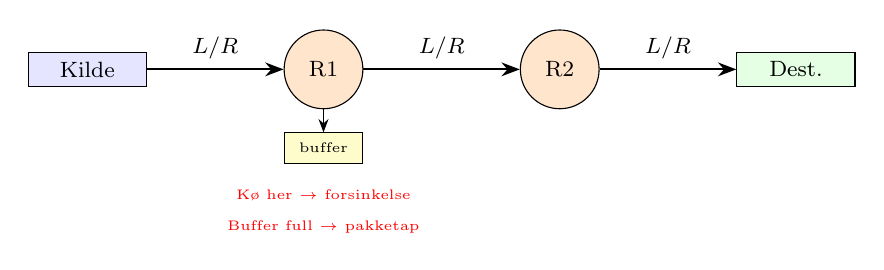
\begin{tikzpicture}[>=Stealth, font=\footnotesize]
    \node[rectangle, draw, fill=blue!10, minimum width=1.5cm] (src) at (0,0) {Kilde};
    \node[circle, draw, fill=orange!20, minimum size=1cm] (r1) at (3,0) {R1};
    \node[circle, draw, fill=orange!20, minimum size=1cm] (r2) at (6,0) {R2};
    \node[rectangle, draw, fill=green!10, minimum width=1.5cm] (dst) at (9,0) {Dest.};

    \draw[->, thick] (src) -- (r1) node[midway, above] {$L/R$};
    \draw[->, thick] (r1) -- (r2) node[midway, above] {$L/R$};
    \draw[->, thick] (r2) -- (dst) node[midway, above] {$L/R$};

    % Buffer illustration
    \draw[fill=yellow!20] (2.5, -0.8) rectangle (3.5, -1.2);
    \node[font=\tiny] at (3, -1) {buffer};
    \draw[->] (3, -0.5) -- (3, -0.8);

    \node[text=red, font=\tiny] at (3, -1.6) {K\o\ her $\rightarrow$ forsinkelse};
    \node[text=red, font=\tiny] at (3, -2.0) {Buffer full $\rightarrow$ pakketap};
\end{tikzpicture}
\end{center}

\textbf{K\o dannelse og pakketap:} Hvis pakker ankommer raskere enn de kan sendes videre, legges de i \textbf{buffer} (k\o). Hvis bufferen er full, \textbf{droppes} pakkene (tap).

\subsection{Kretssvitsjing (Circuit Switching)}

\begin{center}
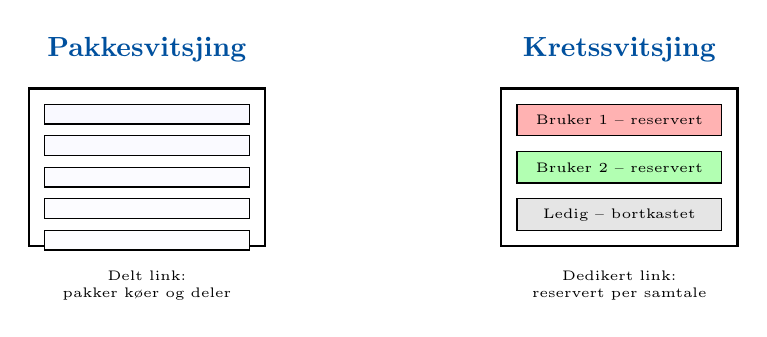
\begin{tikzpicture}[font=\footnotesize]
    % Packet switching
    \node[font=\bfseries, text=ntnu] at (-3, 3) {Pakkesvitsjing};
    \draw[thick] (-4.5, 2.5) rectangle (-1.5, 0.5);
    \foreach \y in {2.3, 1.9, 1.5, 1.1, 0.7} {
        \draw[fill=blue!\y 0!white] (-4.3, \y) rectangle (-1.7, \y-0.25);
    }
    \node[font=\tiny, text width=2.5cm, align=center] at (-3, 0) {Delt link:\\pakker k\o er og deler};

    % Circuit switching
    \node[font=\bfseries, text=ntnu] at (3, 3) {Kretssvitsjing};
    \draw[thick] (1.5, 2.5) rectangle (4.5, 0.5);
    \draw[fill=red!30] (1.7, 2.3) rectangle (4.3, 1.9);
    \node[font=\tiny] at (3, 2.1) {Bruker 1 -- reservert};
    \draw[fill=green!30] (1.7, 1.7) rectangle (4.3, 1.3);
    \node[font=\tiny] at (3, 1.5) {Bruker 2 -- reservert};
    \draw[fill=gray!20] (1.7, 1.1) rectangle (4.3, 0.7);
    \node[font=\tiny] at (3, 0.9) {Ledig -- bortkastet};
    \node[font=\tiny, text width=2.5cm, align=center] at (3, 0) {Dedikert link:\\reservert per samtale};
\end{tikzpicture}
\end{center}

\begin{center}
\begin{tabular}{lcc}
\toprule
& \textbf{Pakkesvitsjing} & \textbf{Kretssvitsjing} \\
\midrule
Ressursdeling & Ja (statistisk multipleksing) & Nei (reservert) \\
Garanti & Ingen & Ja (fast b\aa ndbredde) \\
Effektivitet & H\o y (utnytter ledig kapasitet) & Lav (ledig = bortkastet) \\
K\o ing/tap & Ja & Nei \\
Best for & Bursty trafikk (web, e-post) & Konstant trafikk (telefon) \\
\bottomrule
\end{tabular}
\end{center}

\subsubsection{FDM og TDM}

\begin{center}
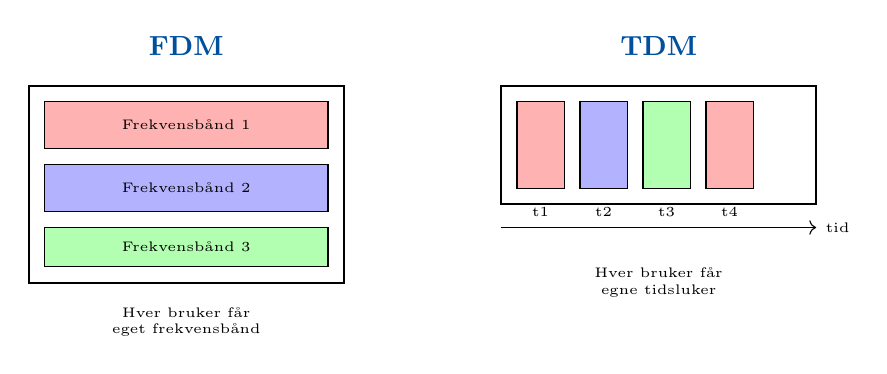
\begin{tikzpicture}[font=\footnotesize]
    % FDM
    \node[font=\bfseries, text=ntnu] at (-3, 2.5) {FDM};
    \draw[thick] (-5, 2) rectangle (-1, -0.5);
    \draw[fill=red!30] (-4.8, 1.8) rectangle (-1.2, 1.2);
    \node[font=\tiny] at (-3, 1.5) {Frekvensb\aa nd 1};
    \draw[fill=blue!30] (-4.8, 1.0) rectangle (-1.2, 0.4);
    \node[font=\tiny] at (-3, 0.7) {Frekvensb\aa nd 2};
    \draw[fill=green!30] (-4.8, 0.2) rectangle (-1.2, -0.3);
    \node[font=\tiny] at (-3, -0.05) {Frekvensb\aa nd 3};
    \node[font=\tiny, text width=3cm, align=center] at (-3, -1) {Hver bruker f\aa r\\eget frekvensb\aa nd};

    % TDM
    \node[font=\bfseries, text=ntnu] at (3, 2.5) {TDM};
    \draw[thick] (1, 2) rectangle (5, 0.5);
    \foreach \x/\col in {1.2/red, 2.0/blue, 2.8/green, 3.6/red} {
        \draw[fill=\col!30] (\x, 1.8) rectangle (\x+0.6, 0.7);
    }
    \draw[->] (1, 0.2) -- (5, 0.2) node[right, font=\tiny] {tid};
    \node[font=\tiny] at (1.5, 0.4) {t1};
    \node[font=\tiny] at (2.3, 0.4) {t2};
    \node[font=\tiny] at (3.1, 0.4) {t3};
    \node[font=\tiny] at (3.9, 0.4) {t4};
    \node[font=\tiny, text width=3cm, align=center] at (3, -0.5) {Hver bruker f\aa r\\egne tidsluker};
\end{tikzpicture}
\end{center}

\subsection{Internettstruktur}

\begin{center}
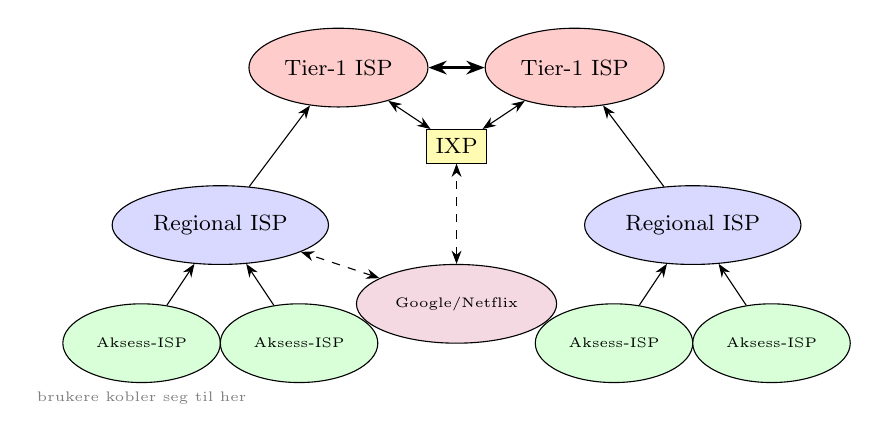
\begin{tikzpicture}[
    isp/.style={ellipse, draw, fill=#1, minimum width=2cm, minimum height=1cm, font=\footnotesize},
    >=Stealth
]
    % Tier 1
    \node[isp=red!20] (t1a) at (-1.5, 3) {Tier-1 ISP};
    \node[isp=red!20] (t1b) at (1.5, 3) {Tier-1 ISP};
    \draw[<->, thick] (t1a) -- (t1b);

    % IXP
    \node[rectangle, draw, fill=yellow!30, font=\footnotesize] (ixp) at (0, 2) {IXP};
    \draw[<->] (t1a) -- (ixp);
    \draw[<->] (t1b) -- (ixp);

    % Regional
    \node[isp=blue!15] (r1) at (-3, 1) {Regional ISP};
    \node[isp=blue!15] (r2) at (3, 1) {Regional ISP};
    \draw[->] (r1) -- (t1a);
    \draw[->] (r2) -- (t1b);

    % Access
    \node[isp=green!15] (a1) at (-4, -0.5) {\tiny Aksess-ISP};
    \node[isp=green!15] (a2) at (-2, -0.5) {\tiny Aksess-ISP};
    \node[isp=green!15] (a3) at (2, -0.5) {\tiny Aksess-ISP};
    \node[isp=green!15] (a4) at (4, -0.5) {\tiny Aksess-ISP};
    \draw[->] (a1) -- (r1);
    \draw[->] (a2) -- (r1);
    \draw[->] (a3) -- (r2);
    \draw[->] (a4) -- (r2);

    % Content provider
    \node[isp=purple!15] (goog) at (0, 0) {\tiny Google/Netflix};
    \draw[<->, dashed] (goog) -- (ixp);
    \draw[<->, dashed] (goog) -- (r1);

    % Labels
    \node[font=\tiny, text=gray] at (-4, -1.2) {brukere kobler seg til her};
\end{tikzpicture}
\end{center}

\begin{itemize}[noitemsep]
    \item \textbf{Aksess-ISP}: Gir brukere tilgang (Telenor, Altibox, etc.)
    \item \textbf{Regionale ISP}: Kobler aksess-ISP-er sammen
    \item \textbf{Tier-1 ISP}: Store, globale nettverk (f.eks.\ Telenor, AT\&T)
    \item \textbf{IXP} (Internet Exchange Point): Kobler ISP-er direkte
    \item \textbf{Content provider networks} (Google, Netflix): Bygger egne nettverk
\end{itemize}

%=============================================================================
\section{Ytelse: Forsinkelse, Tap og Throughput}
%=============================================================================

\subsection{Fire typer forsinkelse}

\begin{formulabox}[Total nodal delay]
\[
d_{\text{nodal}} = d_{\text{proc}} + d_{\text{queue}} + d_{\text{trans}} + d_{\text{prop}}
\]
\end{formulabox}

\begin{center}
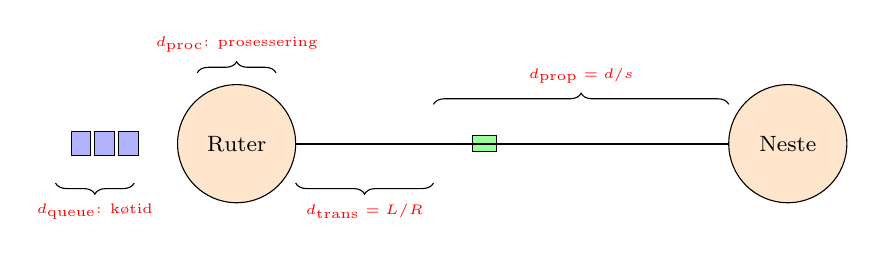
\begin{tikzpicture}[>=Stealth, font=\footnotesize]
    % Router
    \node[circle, draw, fill=orange!20, minimum size=1.5cm] (r1) at (0,0) {Ruter};
    \node[circle, draw, fill=orange!20, minimum size=1.5cm] (r2) at (7,0) {Neste};

    % Packets in queue
    \foreach \x in {-1.5, -1.8, -2.1} {
        \draw[fill=blue!30] (\x, -0.15) rectangle (\x+0.25, 0.15);
    }

    % Packet on link
    \draw[fill=green!40] (3, -0.1) rectangle (3.3, 0.1);

    % Link
    \draw[thick] (0.75, 0) -- (6.25, 0);

    % Braces and labels
    \draw[decorate, decoration={brace,amplitude=4pt,mirror}] (-2.3, -0.5) -- (-1.3, -0.5)
        node[midway, below, yshift=-4pt, font=\tiny, text=red] {$d_{\text{queue}}$: k\o tid};

    \draw[decorate, decoration={brace,amplitude=4pt}] (-0.5, 0.9) -- (0.5, 0.9)
        node[midway, above, yshift=4pt, font=\tiny, text=red] {$d_{\text{proc}}$: prosessering};

    \draw[decorate, decoration={brace,amplitude=4pt,mirror}] (0.75, -0.5) -- (2.5, -0.5)
        node[midway, below, yshift=-4pt, font=\tiny, text=red] {$d_{\text{trans}} = L/R$};

    \draw[decorate, decoration={brace,amplitude=4pt}] (2.5, 0.5) -- (6.25, 0.5)
        node[midway, above, yshift=4pt, font=\tiny, text=red] {$d_{\text{prop}} = d/s$};
\end{tikzpicture}
\end{center}

\begin{center}
\begin{tabular}{llll}
\toprule
\textbf{Forsinkelse} & \textbf{Formel} & \textbf{Avhenger av} & \textbf{Typisk} \\
\midrule
$d_{\text{proc}}$ -- Prosessering & -- & Bitfeilsjekk, velge link & $< 1$ ms \\
$d_{\text{queue}}$ -- K\o & -- & Trafikkintensitet & varierer \\
$d_{\text{trans}}$ -- Overf\o ring & $L/R$ & Pakkest\o rrelse, linkrate & $\mu$s--ms \\
$d_{\text{prop}}$ -- Propagering & $d/s$ & Avstand, signalhastighet & $\mu$s--ms \\
\bottomrule
\end{tabular}
\end{center}

\begin{warnbox}[Viktig: Transmission delay $\neq$ Propagation delay!]
\begin{itemize}[noitemsep]
    \item $d_{\text{trans}} = L/R$ -- tid for \aa\ \textbf{dytte alle bits ut p\aa\ linken}
    \item $d_{\text{prop}} = d/s$ -- tid for signalet \aa\ \textbf{reise gjennom linken}
    \item $s \approx 2 \times 10^8$ m/s i fiber (lyshastighet / brytningsindeks 1.47)
\end{itemize}
\textbf{Eksempel:} Trondheim--Oslo (540 km), fiber:\\
$d_{\text{prop}} = 540\,000 / 200\,000\,000 = 2{,}7$ ms\\
Pakke 1500 bytes, link 1 Gbps:\\
$d_{\text{trans}} = 12\,000 / 1\,000\,000\,000 = 0{,}012$ ms
\end{warnbox}

\subsection{Trafikkintensitet og k\o forsinkelse}

\begin{formulabox}[Trafikkintensitet]
\[
\text{Trafikkintensitet} = \frac{L \cdot a}{R}
\]
hvor $L$ = pakkest\o rrelse (bits), $a$ = gjennomsnittlig ankomstrate (pakker/s), $R$ = linkrate (bps).
\end{formulabox}

\begin{center}
\begin{tikzpicture}[font=\footnotesize]
    \draw[->] (0,0) -- (6,0) node[right] {$La/R$};
    \draw[->] (0,0) -- (0,4.5) node[above] {Gjsn. k\o forsinkelse};

    % Curve
    \draw[thick, red, domain=0:0.95, samples=100] plot ({5*\x}, {0.3*\x/(1-\x)});

    % Asymptote
    \draw[dashed, gray] (5, 0) -- (5, 4.5);
    \node[below, font=\tiny] at (5, 0) {1};

    % Annotations
    \node[text=green!50!black, font=\tiny] at (1.5, 0.5) {$La/R \approx 0$: lite k\o};
    \node[text=orange!70!black, font=\tiny, text width=2cm, align=center] at (4, 2.5) {$La/R \to 1$:\\ stor k\o!};
    \node[text=red, font=\tiny, text width=2cm, align=center] at (6.5, 4) {$La/R > 1$:\\ uendelig!};
\end{tikzpicture}
\end{center}

\subsection{Pakketap}

N\aa r en pakke ankommer en ruter med \textbf{full buffer}, blir pakken \textbf{droppet} (tapt). Tapte pakker kan retransmitteres av forrige node, kilde-endesystemet, eller ikke i det hele tatt.

\subsection{Throughput}

\begin{keybox}[Throughput og flaskehals]
\textbf{Throughput}: Rate (bits/tidsenhet) som bits faktisk overf\o res fra sender til mottaker.
\begin{itemize}[noitemsep]
    \item \textbf{Instantaneous throughput}: Rate p\aa\ et gitt tidspunkt
    \item \textbf{Average throughput}: Rate over lengre tid
    \item \textbf{Bottleneck link}: Linken med lavest kapasitet bestemmer ende-til-ende throughput
\end{itemize}
\[
\text{Throughput} = \min(R_s, R_c)
\]
Med 10 samtidige forbindelser som deler en backbone $R$:
\[
\text{Per-connection throughput} = \min(R_c, R_s, R/10)
\]
\end{keybox}

\begin{center}
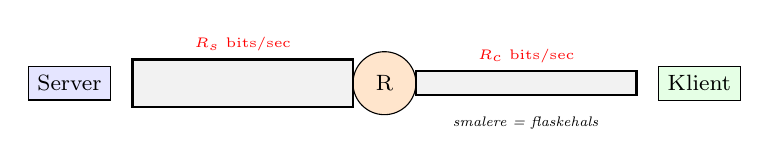
\begin{tikzpicture}[>=Stealth, font=\footnotesize]
    \node[rectangle, draw, fill=blue!10] (srv) at (0, 0) {Server};
    \node[circle, draw, fill=orange!20, minimum size=0.8cm] (r) at (4, 0) {R};
    \node[rectangle, draw, fill=green!10] (cli) at (8, 0) {Klient};

    % Pipes
    \draw[thick, fill=gray!10] (0.8, 0.3) -- (3.6, 0.3) -- (3.6, -0.3) -- (0.8, -0.3) -- cycle;
    \draw[thick, fill=gray!10] (4.4, 0.15) -- (7.2, 0.15) -- (7.2, -0.15) -- (4.4, -0.15) -- cycle;

    \node[font=\tiny, text=red] at (2.2, 0.5) {$R_s$ bits/sec};
    \node[font=\tiny, text=red] at (5.8, 0.35) {$R_c$ bits/sec};
    \node[font=\tiny] at (5.8, -0.5) {\textit{smalere = flaskehals}};
\end{tikzpicture}
\end{center}

\subsection{Traceroute}

\textbf{Traceroute} m\aa ler forsinkelse langs hele ruten fra kilde til destinasjon:
\begin{itemize}[noitemsep]
    \item Sender 3 pakker til hver ruter $i$ p\aa\ veien (med TTL = $i$)
    \item Ruter $i$ returnerer pakken, og senderen m\aa ler tiden
    \item Viser ogs\aa\ pakketap (``* * *'' = ingen respons)
\end{itemize}

%=============================================================================
\section{Sikkerhet}
%=============================================================================

Internett ble opprinnelig designet \textbf{uten} mye sikkerhet -- ``a group of mutually trusting users.''

\begin{center}
\begin{tabular}{lp{7cm}}
\toprule
\textbf{Trussel} & \textbf{Beskrivelse} \\
\midrule
\textbf{Malware} & Virus (krever brukeraksjon), ormer (selvreplikerende), spyware, botnets \\
\textbf{DoS/DDoS} & Overbelaster ressurser med falsk trafikk fra mange kompromitterte maskiner \\
\textbf{Packet sniffing} & Leser alle pakker p\aa\ delt medium (WiFi, Ethernet) med promiscuous NIC \\
\textbf{IP spoofing} & Sender pakker med falsk avsenderadresse \\
\bottomrule
\end{tabular}
\end{center}

\begin{keybox}[Forsvar]
\begin{itemize}[noitemsep]
    \item \textbf{Autentisering} -- beskytter mot spoofing
    \item \textbf{Kryptering} -- beskytter mot sniffing (konfidensialitet)
    \item \textbf{Digitale signaturer} -- sikrer integritet
    \item \textbf{Brannmurer} -- blokkerer uautorisert trafikk
    \item \textbf{VPN} -- begrenser tilgang til ressurser
\end{itemize}
\end{keybox}

%=============================================================================
\section{Protokollag og innkapsling}
%=============================================================================

\subsection{Internettets 5-lags protokollstakk}

\begin{center}
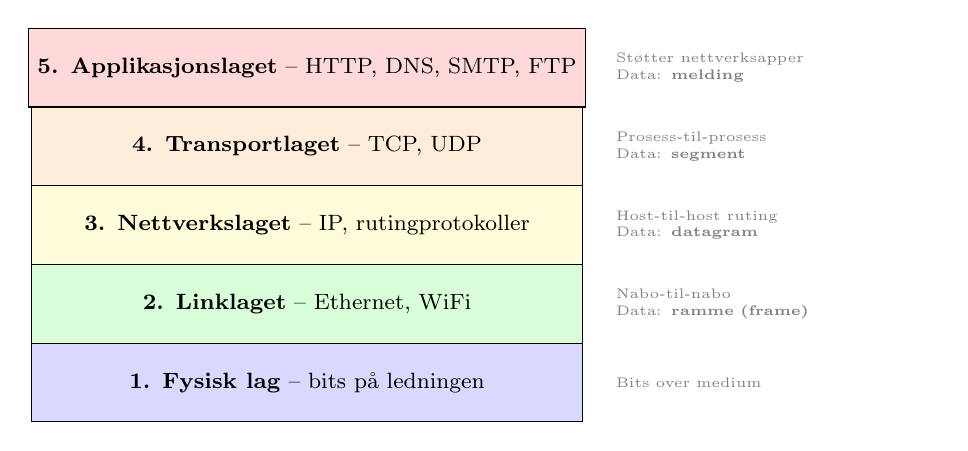
\begin{tikzpicture}[
    layer/.style={rectangle, draw, fill=#1, minimum width=7cm, minimum height=1cm, font=\footnotesize},
    >=Stealth
]
    \node[layer=red!15] (app) at (0, 4) {\textbf{5. Applikasjonslaget} -- HTTP, DNS, SMTP, FTP};
    \node[layer=orange!15] (trans) at (0, 3) {\textbf{4. Transportlaget} -- TCP, UDP};
    \node[layer=yellow!15] (net) at (0, 2) {\textbf{3. Nettverkslaget} -- IP, rutingprotokoller};
    \node[layer=green!15] (link) at (0, 1) {\textbf{2. Linklaget} -- Ethernet, WiFi};
    \node[layer=blue!15] (phys) at (0, 0) {\textbf{1. Fysisk lag} -- bits p\aa\ ledningen};

    % Descriptions on right
    \node[font=\tiny, text=gray, text width=4cm, right] at (3.8, 4) {St\o tter nettverksapper\\Data: \textbf{melding}};
    \node[font=\tiny, text=gray, text width=4cm, right] at (3.8, 3) {Prosess-til-prosess\\Data: \textbf{segment}};
    \node[font=\tiny, text=gray, text width=4cm, right] at (3.8, 2) {Host-til-host ruting\\Data: \textbf{datagram}};
    \node[font=\tiny, text=gray, text width=4cm, right] at (3.8, 1) {Nabo-til-nabo\\Data: \textbf{ramme (frame)}};
    \node[font=\tiny, text=gray, text width=4cm, right] at (3.8, 0) {Bits over medium};
\end{tikzpicture}
\end{center}

\begin{warnbox}[ISO/OSI-modellen har 7 lag]
OSI legger til \textbf{Presentasjon} og \textbf{Sesjon} mellom applikasjon og transport. Disse er i praksis inkludert i applikasjonslaget i Internett-modellen.
\end{warnbox}

\subsection{Innkapsling (Encapsulation)}

\begin{center}
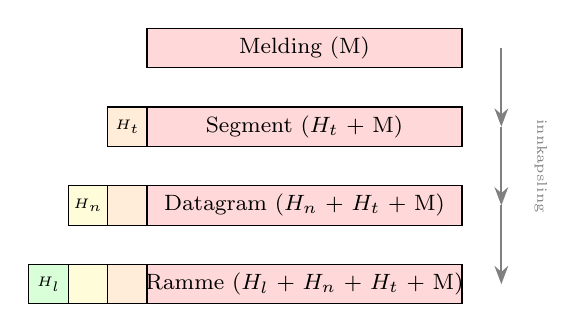
\begin{tikzpicture}[font=\footnotesize, >=Stealth]
    % Application
    \draw[fill=red!15] (0, 4) rectangle (4, 4.5);
    \node at (2, 4.25) {Melding (M)};

    % Transport
    \draw[fill=orange!15] (-0.5, 3) rectangle (0, 3.5);
    \draw[fill=red!15] (0, 3) rectangle (4, 3.5);
    \node[font=\tiny] at (-0.25, 3.25) {$H_t$};
    \node at (2, 3.25) {Segment ($H_t$ + M)};

    % Network
    \draw[fill=yellow!15] (-1, 2) rectangle (-0.5, 2.5);
    \draw[fill=orange!15] (-0.5, 2) rectangle (0, 2.5);
    \draw[fill=red!15] (0, 2) rectangle (4, 2.5);
    \node[font=\tiny] at (-0.75, 2.25) {$H_n$};
    \node at (2, 2.25) {Datagram ($H_n$ + $H_t$ + M)};

    % Link
    \draw[fill=green!15] (-1.5, 1) rectangle (-1, 1.5);
    \draw[fill=yellow!15] (-1, 1) rectangle (-0.5, 1.5);
    \draw[fill=orange!15] (-0.5, 1) rectangle (0, 1.5);
    \draw[fill=red!15] (0, 1) rectangle (4, 1.5);
    \node[font=\tiny] at (-1.25, 1.25) {$H_l$};
    \node at (2, 1.25) {Ramme ($H_l$ + $H_n$ + $H_t$ + M)};

    % Arrows
    \draw[->, thick, gray] (4.5, 4.25) -- (4.5, 3.25);
    \draw[->, thick, gray] (4.5, 3.25) -- (4.5, 2.25);
    \draw[->, thick, gray] (4.5, 2.25) -- (4.5, 1.25);

    \node[font=\tiny, text=gray, rotate=-90] at (5, 2.75) {innkapsling};
\end{tikzpicture}
\end{center}

Hvert lag legger til sin \textbf{header} ($H$) rundt dataene fra laget over. Mottaker fjerner headers i omvendt rekkef\o lge.

\bigskip
\begin{keybox}[Hvorfor lagdeling?]
\begin{itemize}[noitemsep]
    \item Gir \textbf{klar struktur} -- lettere \aa\ designe og vedlikeholde
    \item \textbf{Modularisering} -- kan endre ett lag uten \aa\ p\aa virke andre
    \item Separerer komplekse systemer i h\aa ndterbare deler
\end{itemize}
\end{keybox}

%=============================================================================
\section{Pensumssp\o rsm\aa l -- Kapittel 1}
%=============================================================================

Her er de viktigste sp\o rsm\aa lene fra pensum, organisert etter tema.

\subsection{1.1 Nuts and bolts vs. Service view}

\begin{exambox}[Eksamensssp\o rsm\aa l]
\begin{longtable}{p{6.5cm}p{7cm}}
\toprule
\textbf{Sp\o rsm\aa l} & \textbf{Svar} \\
\midrule
\endhead
Hva er internett if\o lge ``nuts and bolts''? & Et globalt nettverk som kobler sammen milliarder av endesystemer. \\
\midrule
Hva er en ISP? & En internettleverand\o r som gir endesystemer tilgang til internett. \\
\midrule
Hvilke protokoller styrer internett? & TCP/IP. \\
\midrule
Hvem utvikler internettstandardene? & IETF (Internet Engineering Task Force). \\
\midrule
Hva kalles dokumentene som beskriver standardene? & RFC-er (Requests for Comments). \\
\midrule
Hva er internett if\o lge ``services view''? & En plattform som leverer tjenester til applikasjoner. \\
\midrule
Hva er en protokoll? & Et regelsett som definerer format, rekkef\o lge og handlinger for meldinger mellom kommunikasjonsenheter. \\
\bottomrule
\end{longtable}
\end{exambox}

\subsection{1.2 Network Edge}

\begin{exambox}[Eksamensssp\o rsm\aa l]
\begin{longtable}{p{6.5cm}p{7cm}}
\toprule
\textbf{Sp\o rsm\aa l} & \textbf{Svar} \\
\midrule
\endhead
Hvilke to typer verter finnes? & Klienter og servere. \\
\midrule
Hva st\aa r DSL for? & Digital Subscriber Line. \\
\midrule
Er DSL symmetrisk eller asymmetrisk? & Asymmetrisk (h\o yere nedlasting). \\
\midrule
Hva er HFC? & Hybrid Fiber Coax -- kabelnett med fiber + koaks. \\
\midrule
Hva er forskjellen p\aa\ delt og dedikert aksess? & DSL er dedikert, kabel er delt. \\
\midrule
Hva er formelen for packet transmission delay? & $D = L / R$. \\
\midrule
Hva er guided vs.\ unguided media? & Guided: signal i fysisk medium (kobber, fiber). Unguided: signal fritt (radio). \\
\midrule
Hva er fordelene med fiber? & H\o y hastighet, lav feilrate. \\
\bottomrule
\end{longtable}
\end{exambox}

\subsection{1.3 Network Core}

\begin{exambox}[Eksamensssp\o rsm\aa l]
\begin{longtable}{p{6.5cm}p{7cm}}
\toprule
\textbf{Sp\o rsm\aa l} & \textbf{Svar} \\
\midrule
\endhead
Hva er ``store-and-forward''? & Hele pakken m\aa\ ankomme f\o r den kan sendes videre. \\
\midrule
Hva skjer n\aa r bufferen er full? & Pakker droppes (tap). \\
\midrule
Hva er forskjellen p\aa\ pakkesvitsjing og kretssvitsjing? & Krets reserverer fast forbindelse; pakke sender data i sm\aa\ biter som deler linjen. \\
\midrule
Hva er FDM? & Frequency Division Multiplexing -- hver bruker f\aa r eget frekvensb\aa nd. \\
\midrule
Hva er TDM? & Time Division Multiplexing -- hver bruker f\aa r egne tidsluker. \\
\midrule
N\aa r er pakkesvitsjing best? & For bursty trafikk -- noen ganger aktiv, noen ganger ikke. \\
\midrule
Hva er tier-1 ISP? & Store, globale nettverk (f.eks.\ Telenor, AT\&T). \\
\midrule
Hva er IXP? & Internet Exchange Point -- kobler ISP-er direkte. \\
\bottomrule
\end{longtable}
\end{exambox}

\subsection{1.4 Performance}

\begin{exambox}[Eksamensssp\o rsm\aa l]
\begin{longtable}{p{6.5cm}p{7cm}}
\toprule
\textbf{Sp\o rsm\aa l} & \textbf{Svar} \\
\midrule
\endhead
Hva er de fire forsinkelsestypene? & Processing, queueing, transmission ($L/R$), propagation ($d/s$). \\
\midrule
Hva er trafikkintensitet? & $(L \times a) / R$ -- forholdet mellom ankomstrate og tjenesterate. \\
\midrule
Hva skjer n\aa r $La/R > 1$? & Mer arbeid ankommer enn kan h\aa ndteres; forsinkelse $\to \infty$. \\
\midrule
Hva er throughput? & Rate bits faktisk overf\o res fra sender til mottaker. \\
\midrule
Hva er bottleneck link? & Linken med lavest kapasitet -- bestemmer ende-til-ende throughput. \\
\bottomrule
\end{longtable}
\end{exambox}

\subsection{1.5 Lagdeling og 1.6 Sikkerhet}

\begin{exambox}[Eksamensssp\o rsm\aa l]
\begin{longtable}{p{6.5cm}p{7cm}}
\toprule
\textbf{Sp\o rsm\aa l} & \textbf{Svar} \\
\midrule
\endhead
Hvor mange lag i internett-protokollstakken? & Fem: applikasjon, transport, nettverk, link, fysisk. \\
\midrule
Hva er innkapsling? & Pakke data med headers fra hvert lag. \\
\midrule
Hva er packet sniffing? & Lese alle pakker p\aa\ delt nettverk. \\
\midrule
Hva er IP spoofing? & Sende pakker med falsk avsenderadresse. \\
\midrule
Hva er et DoS-angrep? & Gj\o re ressurser utilgjengelige ved \aa\ overbelaste med falsk trafikk. \\
\midrule
Hva beskytter mot sniffing? & Kryptering. \\
\midrule
Hva beskytter mot spoofing? & Autentisering. \\
\bottomrule
\end{longtable}
\end{exambox}

%=============================================================================
\section{Oppsummering -- viktige formler}
%=============================================================================

\begin{formulabox}[Formler du m\aa\ kunne]
\begin{align}
d_{\text{trans}} &= \frac{L}{R} & &\text{Transmission delay (pakkest\o rrelse / linkrate)} \\[6pt]
d_{\text{prop}} &= \frac{d}{s} & &\text{Propagation delay (avstand / signalhastighet)} \\[6pt]
d_{\text{nodal}} &= d_{\text{proc}} + d_{\text{queue}} + d_{\text{trans}} + d_{\text{prop}} & &\text{Total forsinkelse per node} \\[6pt]
\text{Trafikk\-intensitet} &= \frac{L \cdot a}{R} & &\text{Ankomstrate vs.\ tjenesterate} \\[6pt]
\text{Throughput} &= \min(R_s, R_c) & &\text{Bestemt av flaskehalsen}
\end{align}

\textbf{Verdier \aa\ huske:}
\begin{itemize}[noitemsep]
    \item Signalhastighet i fiber: $s \approx 2 \times 10^8$ m/s
    \item Lyshastighet: $c = 3 \times 10^8$ m/s (fiber har brytningsindeks $\approx 1{,}47$)
    \item 1 byte = 8 bits
\end{itemize}
\end{formulabox}


% ============================================================
%  CHAPTER 2
% ============================================================
\chapterdivider{2}{Chapter 2: The Application Layer}
\section{Prinsipper for nettverksapplikasjoner (2.1)}
%=============================================================================

\subsection{Applikasjonsarkitekturer}

To dominerende arkitekturer for nettverksapplikasjoner:

\begin{keybox}[Klient-server vs. Peer-to-Peer (P2P)]
\textbf{Klient-server:}
\begin{itemize}[noitemsep]
    \item Serveren er \textbf{alltid p\aa} (always-on) med fast (permanent) IP-adresse
    \item Klienter kontakter serveren, kan ha dynamisk IP
    \item Klienter kommuniserer \textbf{ikke direkte} med hverandre
    \item Eksempler: HTTP, IMAP, FTP
    \item Skalering: flere servere i datasentre
\end{itemize}

\textbf{Peer-to-Peer (P2P):}
\begin{itemize}[noitemsep]
    \item \textbf{Ingen} dedikert server -- endesystemer kommuniserer direkte
    \item Peers tilbyr tjenester til hverandre
    \item \textbf{Selvskaler\-ende}: nye peers bringer b\aa de kapasitet og ettersp\o rsel
    \item Utfordring: peers er intermittent tilkoblet, endrer IP
    \item Eksempler: BitTorrent, Skype, KanKan
\end{itemize}
\end{keybox}

\begin{center}
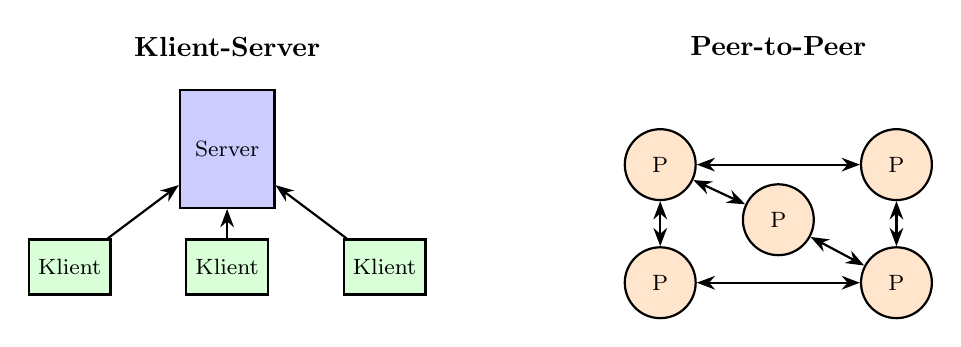
\begin{tikzpicture}[
    server/.style={rectangle, draw, fill=blue!20, minimum width=1.2cm, minimum height=1.5cm, font=\footnotesize},
    client/.style={rectangle, draw, fill=green!15, minimum width=1cm, minimum height=0.7cm, font=\footnotesize},
    peer/.style={circle, draw, fill=orange!20, minimum size=0.9cm, font=\footnotesize},
    >=Stealth, thick
]
    % Client-Server
    \node[font=\bfseries] at (-3.5,2.5) {Klient-Server};
    \node[server] (srv) at (-3.5,1.2) {Server};
    \node[client] (c1) at (-5.5,-0.3) {Klient};
    \node[client] (c2) at (-3.5,-0.3) {Klient};
    \node[client] (c3) at (-1.5,-0.3) {Klient};
    \draw[->] (c1) -- (srv);
    \draw[->] (c2) -- (srv);
    \draw[->] (c3) -- (srv);

    % P2P
    \node[font=\bfseries] at (3.5,2.5) {Peer-to-Peer};
    \node[peer] (p1) at (2,1) {P};
    \node[peer] (p2) at (5,1) {P};
    \node[peer] (p3) at (2,-0.5) {P};
    \node[peer] (p4) at (5,-0.5) {P};
    \node[peer] (p5) at (3.5,0.3) {P};
    \draw[<->] (p1) -- (p2);
    \draw[<->] (p1) -- (p3);
    \draw[<->] (p2) -- (p4);
    \draw[<->] (p3) -- (p4);
    \draw[<->] (p1) -- (p5);
    \draw[<->] (p5) -- (p4);
\end{tikzpicture}
\end{center}

\subsection{Prosesser og socketer}

\begin{keybox}[Prosesser og kommunikasjon]
\begin{itemize}[noitemsep]
    \item En \textbf{prosess} er et program som kj\o rer p\aa\ en vert (host)
    \item P\aa\ \textbf{samme} vert: inter-prosess kommunikasjon (IPC)
    \item P\aa\ \textbf{ulike} verter: utveksling av \textbf{meldinger}
    \item \textbf{Klientprosess}: initierer kommunikasjon
    \item \textbf{Serverprosess}: venter p\aa\ \aa\ bli kontaktet
\end{itemize}
\end{keybox}

\begin{keybox}[Socket -- ``D\o ren'' mellom applikasjon og transport]
En \textbf{socket} er grensesnittet mellom applikasjonslaget og transportlaget. Prosessen sender/mottar meldinger gjennom sin socket.
\begin{itemize}[noitemsep]
    \item To socketer involvert: en p\aa\ hver side
    \item Applikasjonsutvikler kontrollerer alt \textbf{over} socketen
    \item OS kontrollerer alt \textbf{under} socketen (transport, nettverk, link, fysisk)
\end{itemize}
\end{keybox}

\begin{center}
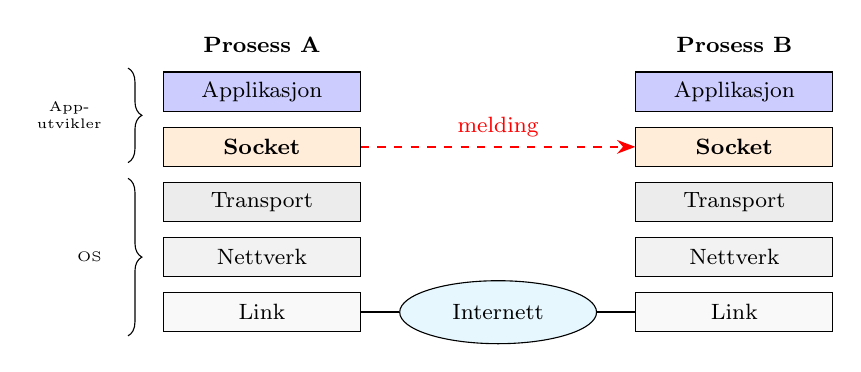
\begin{tikzpicture}[
    layer/.style={rectangle, draw, minimum width=2.5cm, minimum height=0.5cm, font=\footnotesize},
    >=Stealth
]
    % Left host
    \node[layer, fill=blue!20] (app1) at (0,2.5) {Applikasjon};
    \node[layer, fill=orange!15] (sock1) at (0,1.8) {\textbf{Socket}};
    \node[layer, fill=gray!15] (trans1) at (0,1.1) {Transport};
    \node[layer, fill=gray!10] (net1) at (0,0.4) {Nettverk};
    \node[layer, fill=gray!5] (link1) at (0,-0.3) {Link};
    \node[font=\footnotesize\bfseries] at (0,3.1) {Prosess A};

    % Right host
    \node[layer, fill=blue!20] (app2) at (6,2.5) {Applikasjon};
    \node[layer, fill=orange!15] (sock2) at (6,1.8) {\textbf{Socket}};
    \node[layer, fill=gray!15] (trans2) at (6,1.1) {Transport};
    \node[layer, fill=gray!10] (net2) at (6,0.4) {Nettverk};
    \node[layer, fill=gray!5] (link2) at (6,-0.3) {Link};
    \node[font=\footnotesize\bfseries] at (6,3.1) {Prosess B};

    % Internet
    \node[ellipse, draw, fill=cyan!10, minimum width=2.5cm, minimum height=0.8cm, font=\footnotesize] (inet) at (3,-0.3) {Internett};
    \draw[thick] (link1.east) -- (inet.west);
    \draw[thick] (inet.east) -- (link2.west);

    % Message arrow
    \draw[->, thick, red, dashed] (sock1.east) -- node[above, font=\footnotesize, text=red] {melding} (sock2.west);

    % Braces
    \draw[decorate, decoration={brace, amplitude=5pt}] (-1.7,2.8) -- (-1.7,1.6) node[midway, left=6pt, font=\tiny, align=center] {App-\\utvikler};
    \draw[decorate, decoration={brace, amplitude=5pt}] (-1.7,1.4) -- (-1.7,-0.6) node[midway, left=6pt, font=\tiny, align=center] {OS};
\end{tikzpicture}
\end{center}

\subsection{Adressering av prosesser}

\begin{warnbox}[IP-adresse alene er ikke nok!]
En prosess identifiseres unikt med \textbf{IP-adresse + portnummer}.
\begin{itemize}[noitemsep]
    \item IP-adressen identifiserer \textbf{verten}
    \item Portnummeret identifiserer \textbf{prosessen} p\aa\ verten
    \item Velkjente porter: HTTP = \textbf{80}, Mail (SMTP) = \textbf{25}, DNS = \textbf{53}
\end{itemize}
\end{warnbox}

\subsection{Applikasjonslagsprotokoller}

En applikasjonslagsprotokoll definerer:
\begin{enumerate}[noitemsep]
    \item \textbf{Meldingstyper}: request og response
    \item \textbf{Syntaks}: feltene i meldingen og deres format
    \item \textbf{Semantikk}: betydningen av feltene
    \item \textbf{Regler}: n\aa r prosesser sender/responderer
\end{enumerate}

\textbf{\AA pne protokoller}: definert i RFCer, tilgjengelig for alle (HTTP, SMTP).\\
\textbf{Propriet\ae re protokoller}: private (Skype, Zoom).

\subsection{Transporttjenestekrav}

\begin{center}
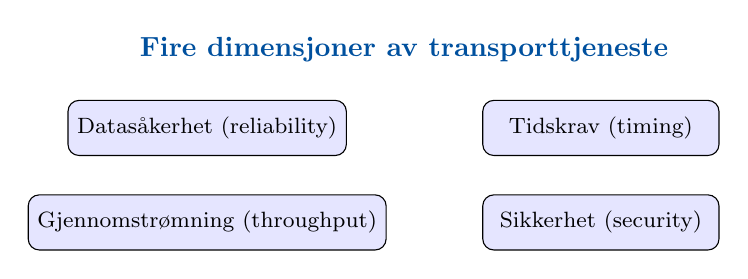
\begin{tikzpicture}[
    box/.style={rectangle, draw, fill=blue!10, minimum width=3cm, minimum height=0.7cm, font=\footnotesize, rounded corners},
    >=Stealth
]
    \node[box] (rel) at (0,0) {Datas\aa kerhet (reliability)};
    \node[box] (tim) at (5,0) {Tidskrav (timing)};
    \node[box] (thr) at (0,-1.2) {Gjennomstr\o mning (throughput)};
    \node[box] (sec) at (5,-1.2) {Sikkerhet (security)};
    \node[font=\bfseries, text=ntnu] at (2.5,1) {Fire dimensjoner av transporttjeneste};
\end{tikzpicture}
\end{center}

\begin{keybox}[TCP vs. UDP -- Hva tilbyr de?]
\begin{tabular}{lcc}
\toprule
\textbf{Egenskap} & \textbf{TCP} & \textbf{UDP} \\
\midrule
P\aa litelig dataoverf\o ring & \checkmark & $\times$ \\
Flytkontroll & \checkmark & $\times$ \\
Metningskontroll & \checkmark & $\times$ \\
Tilkoblingsoppsett & \checkmark & $\times$ \\
Tidskrav (timing) & $\times$ & $\times$ \\
Min. gjennomstr\o mning & $\times$ & $\times$ \\
Sikkerhet (innebygd) & $\times$ & $\times$ \\
\bottomrule
\end{tabular}
\vspace{0.3em}

\textbf{TLS} gir kryptert TCP-tilkobling, dataintegritet og autentisering.
\end{keybox}

%--- Exam questions 2.1 ---
\begin{exambox}[Eksamenssp\o rsm\aa l -- 2.1 Prinsipper]
\small
\begin{longtable}{p{7cm}p{7cm}}
\toprule
\textbf{Sp\o rsm\aa l} & \textbf{Svar} \\
\midrule
\endhead
What is a server in the client-server paradigm? & An always-on host with a permanent IP, often in data centers. \\
\midrule
What is a client in the client-server paradigm? & A device that contacts servers, may be intermittently connected and have dynamic IPs. \\
\midrule
Can clients communicate directly in client-server? & No. \\
\midrule
What is peer-to-peer architecture? & A model where end systems (peers) communicate directly without a central server. \\
\midrule
What is a socket? & An interface for sending and receiving process messages, connecting an app on one computer to an app on another. \\
\midrule
Why is an IP address alone not enough? & Because multiple processes can run on the same host. \\
\midrule
What does an application-layer protocol define? & Message types, syntax, semantics, and communication rules. \\
\midrule
What does TCP provide? & Reliable transport, flow control, congestion control, connection setup. \\
\midrule
What does UDP provide? & Unreliable data transfer with no added features. \\
\midrule
What does TLS provide? & Encrypted TCP connections, data integrity, and end-point authentication. \\
\bottomrule
\end{longtable}
\end{exambox}


\newpage
%=============================================================================
\section{Web og HTTP (2.2)}
%=============================================================================

\subsection{Grunnleggende om HTTP}

\begin{keybox}[HTTP -- HyperText Transfer Protocol]
\begin{itemize}[noitemsep]
    \item En \textbf{webside} best\aa r av en base-HTML-fil og refererte objekter (bilder, skript, etc.)
    \item HTTP f\o lger \textbf{klient-server}-modellen
    \item Bruker \textbf{TCP} (port \textbf{80})
    \item HTTP er \textbf{stateless} -- serveren lagrer ikke informasjon om tidligere foresp\o rsler
\end{itemize}
\end{keybox}

\subsection{Persistent vs. Non-persistent HTTP}

\begin{center}
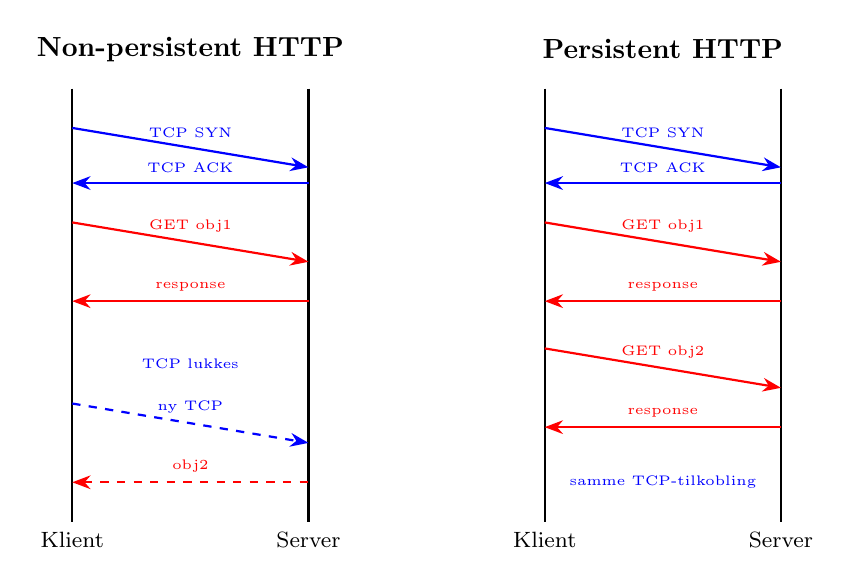
\begin{tikzpicture}[
    >=Stealth, thick,
    box/.style={rectangle, draw, fill=blue!10, minimum width=2.5cm, minimum height=0.8cm, font=\small}
]
    % Non-persistent
    \node[font=\bfseries] at (-3,4) {Non-persistent HTTP};
    \draw[thick] (-4.5,3.5) -- (-4.5,-2) node[below, font=\footnotesize] {Klient};
    \draw[thick] (-1.5,3.5) -- (-1.5,-2) node[below, font=\footnotesize] {Server};

    % Connection 1
    \draw[->, blue] (-4.5,3) -- (-1.5,2.5) node[midway, above, font=\tiny] {TCP SYN};
    \draw[<-, blue] (-4.5,2.3) -- (-1.5,2.3) node[midway, above, font=\tiny] {TCP ACK};
    \draw[->, red] (-4.5,1.8) -- (-1.5,1.3) node[midway, above, font=\tiny] {GET obj1};
    \draw[<-, red] (-4.5,0.8) -- (-1.5,0.8) node[midway, above, font=\tiny] {response};
    \node[font=\tiny, text=blue] at (-3,-0.0) {TCP lukkes};

    % Connection 2
    \draw[->, blue, dashed] (-4.5,-0.5) -- (-1.5,-1) node[midway, above, font=\tiny] {ny TCP};
    \draw[<-, red, dashed] (-4.5,-1.5) -- (-1.5,-1.5) node[midway, above, font=\tiny] {obj2};

    % Persistent
    \node[font=\bfseries] at (3,4) {Persistent HTTP};
    \draw[thick] (1.5,3.5) -- (1.5,-2) node[below, font=\footnotesize] {Klient};
    \draw[thick] (4.5,3.5) -- (4.5,-2) node[below, font=\footnotesize] {Server};

    \draw[->, blue] (1.5,3) -- (4.5,2.5) node[midway, above, font=\tiny] {TCP SYN};
    \draw[<-, blue] (1.5,2.3) -- (4.5,2.3) node[midway, above, font=\tiny] {TCP ACK};
    \draw[->, red] (1.5,1.8) -- (4.5,1.3) node[midway, above, font=\tiny] {GET obj1};
    \draw[<-, red] (1.5,0.8) -- (4.5,0.8) node[midway, above, font=\tiny] {response};
    \draw[->, red] (1.5,0.2) -- (4.5,-0.3) node[midway, above, font=\tiny] {GET obj2};
    \draw[<-, red] (1.5,-0.8) -- (4.5,-0.8) node[midway, above, font=\tiny] {response};
    \node[font=\tiny, text=blue] at (3,-1.5) {samme TCP-tilkobling};
\end{tikzpicture}
\end{center}

\begin{warnbox}[Non-persistent HTTP: Tid per objekt]
Hvert objekt krever: \textbf{2 RTT + filoverf\o ringstid}
\begin{itemize}[noitemsep]
    \item 1 RTT for TCP-tilkobling
    \item 1 RTT for HTTP request/response
    \item Problemer: h\o y RTT-kostnad, OS-overhead for mange TCP-tilkoblinger
\end{itemize}
\end{warnbox}

\begin{formulabox}[Response-tid for Non-persistent HTTP]
$$T_{\text{non-pers}} = 2 \cdot RTT + T_{\text{fil}}$$
For en webside med base-HTML + $n$ objekter:
$$T_{\text{total}} = (n+1) \times (2 \cdot RTT + T_{\text{fil}})$$
\end{formulabox}

\subsection{HTTP-meldinger}

\textbf{To typer:} Request og Response.

\begin{keybox}[HTTP Request -- viktige metoder]
\begin{tabular}{ll}
\toprule
\textbf{Metode} & \textbf{Beskrivelse} \\
\midrule
\texttt{GET} & Henter ressurs; data i URL etter ``?'' \\
\texttt{POST} & Sender data i meldingskroppen (entity body) \\
\texttt{HEAD} & Som GET, men returnerer kun headers \\
\texttt{PUT} & Laster opp / erstatter en fil p\aa\ serveren \\
\bottomrule
\end{tabular}
\end{keybox}

\begin{keybox}[HTTP Response -- statuskoder]
\begin{tabular}{ll}
\toprule
\textbf{Kode} & \textbf{Betydning} \\
\midrule
\texttt{200 OK} & Foresp\o rselen var vellykket \\
\texttt{301 Moved Permanently} & Objektet har ny permanent URL \\
\texttt{400 Bad Request} & Serveren forsto ikke meldingen \\
\texttt{404 Not Found} & Dokumentet finnes ikke p\aa\ serveren \\
\bottomrule
\end{tabular}
\end{keybox}

\subsection{Cookies}

\begin{keybox}[Cookies -- Tilstandsinformasjon i stateless HTTP]
Cookies brukes for \aa\ holde tilstand p\aa\ tvers av HTTP-foresp\o rsler.

\textbf{Fire komponenter:}
\begin{enumerate}[noitemsep]
    \item Cookie-header i HTTP \textbf{response} (Set-Cookie)
    \item Cookie-header i HTTP \textbf{request} (Cookie)
    \item Cookie-fil p\aa\ \textbf{klienten} (lagret av nettleseren)
    \item \textbf{Database} p\aa\ serveren
\end{enumerate}

Bruksomr\aa der: autorisasjon, handlekurver, anbefalinger, sesjonstilstand.
\end{keybox}

\subsection{Web Caching (Proxy Server)}

\begin{keybox}[Web Cache -- M\aa l: tilfredsstille foresp\o rsler uten origin server]
\begin{itemize}[noitemsep]
    \item Nettleseren sender \textbf{alle} HTTP-foresp\o rsler til cachen
    \item Finnes objektet? $\rightarrow$ cache returnerer det direkte
    \item Finnes det ikke? $\rightarrow$ cache henter fra origin server, cacher det, returnerer
    \item Cachen fungerer b\aa de som \textbf{server} (for klienten) og \textbf{klient} (for origin server)
\end{itemize}
\end{keybox}

\begin{center}
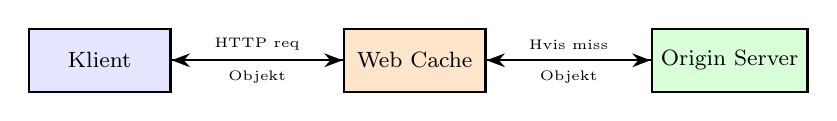
\begin{tikzpicture}[
    box/.style={rectangle, draw, fill=blue!10, minimum width=1.8cm, minimum height=0.8cm, font=\footnotesize},
    >=Stealth, thick
]
    \node[box] (client) at (0,0) {Klient};
    \node[box, fill=orange!20] (cache) at (4,0) {Web Cache};
    \node[box, fill=green!15] (origin) at (8,0) {Origin Server};

    \draw[->] (client) -- node[above, font=\tiny] {HTTP req} (cache);
    \draw[->] (cache) -- node[above, font=\tiny] {Hvis miss} (origin);
    \draw[<-, below] (cache) -- node[below, font=\tiny] {Objekt} (origin);
    \draw[<-] (client) -- node[below, font=\tiny] {Objekt} (cache);
\end{tikzpicture}
\end{center}

\textbf{Fordeler med caching:}
\begin{enumerate}[noitemsep]
    \item Reduserer responstid for klienten
    \item Reduserer trafikk p\aa\ institusjonens aksesslink
    \item Billigere enn \aa\ oppgradere aksesslinken
\end{enumerate}

\begin{keybox}[Conditional GET -- Unng\aa\ un\o dvendig overf\o ring]
\begin{itemize}[noitemsep]
    \item Request-header: \texttt{If-Modified-Since: <dato>}
    \item Svar hvis uendret: \texttt{304 Not Modified} (ingen data sendes)
    \item Svar hvis endret: \texttt{200 OK} + oppdatert objekt
\end{itemize}
\end{keybox}

\subsection{HTTP/2 og HTTP/3}

\begin{keybox}[HTTP/2 -- Redusere forsinkelse]
\begin{itemize}[noitemsep]
    \item M\aa l: redusere delay i multi-objekt foresp\o rsler
    \item \textbf{Prioritetsbasert overf\o ring}: viktige objekter f\o rst
    \item \textbf{Server push}: serveren kan sende objekter klienten ikke har bedt om
    \item \textbf{Framing}: objekter deles i frames som \textbf{interleaves} $\rightarrow$ reduserer HOL-blocking
\end{itemize}
\end{keybox}

\begin{warnbox}[HOL-blocking (Head-of-Line)]
I HTTP/1.1 m\aa\ objekter sendes sekvensielt. Et stort objekt blokkerer sm\aa\ objekter bak i k\o en. HTTP/2 l\o ser dette med frame-interleaving.
\end{warnbox}

\begin{keybox}[HTTP/3 -- L\o ser TCP-begrensninger]
\begin{itemize}[noitemsep]
    \item Bruker \textbf{UDP} (via QUIC) i stedet for TCP
    \item Per-objekt feil- og metningskontroll
    \item Innebygd sikkerhet
    \item L\o ser problemet med at \textit{pakketap p\aa\ TCP p\aa virker alle objekter}
\end{itemize}
\end{keybox}

%--- Exam questions 2.2 ---
\begin{exambox}[Eksamenssp\o rsm\aa l -- 2.2 Web og HTTP]
\small
\begin{longtable}{p{7cm}p{7cm}}
\toprule
\textbf{Sp\o rsm\aa l} & \textbf{Svar} \\
\midrule
\endhead
What is HTTP? & The application layer protocol used by the web to transfer data. \\
\midrule
Which protocol does HTTP use underneath? & TCP. \\
\midrule
Is HTTP stateful or stateless? & Stateless -- the server does not store past requests. \\
\midrule
How many RTTs per object in non-persistent HTTP? & 2 RTTs + file transmission time. \\
\midrule
What does the POST method do? & Sends user input in the entity body of the request. \\
\midrule
What does 404 mean? & Not Found -- the requested document doesn't exist. \\
\midrule
What are the four components of cookies? & 1) Cookie in response, 2) Cookie in request, 3) File on client, 4) Database on server. \\
\midrule
What is the goal of web caching? & To satisfy client requests without involving the origin server. \\
\midrule
What is a Conditional GET used for? & To avoid sending an object if the cached version is still up-to-date. \\
\midrule
What is the main goal of HTTP/2? & To decrease delay in multi-object HTTP requests. \\
\midrule
How does HTTP/2 reduce HOL blocking? & By dividing objects into frames and interleaving their transmission. \\
\midrule
How does HTTP/3 address HTTP/2 limitations? & Uses UDP for per-object error and congestion control, includes security. \\
\bottomrule
\end{longtable}
\end{exambox}


\newpage
%=============================================================================
\section{E-post: SMTP og IMAP (2.3)}
%=============================================================================

\subsection{E-postsystemets komponenter}

\begin{keybox}[Tre hovedkomponenter i e-postsystemet]
\begin{enumerate}[noitemsep]
    \item \textbf{User agent (UA)}: skrive, redigere og lese e-post
    \item \textbf{Mailserver}: lagrer innkommende meldinger (mailbox) og utg\aa ende meldinger (message queue)
    \item \textbf{SMTP}: protokollen for \aa\ sende e-post mellom mailservere
\end{enumerate}
\end{keybox}

\begin{center}
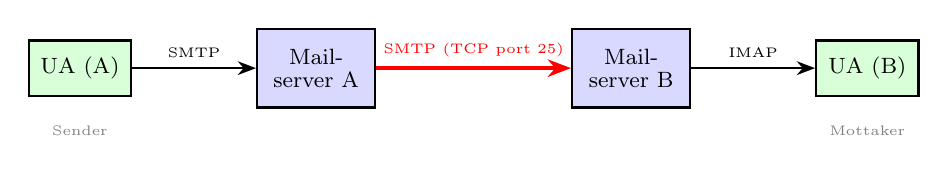
\begin{tikzpicture}[
    ua/.style={rectangle, draw, fill=green!15, minimum width=1.3cm, minimum height=0.7cm, font=\footnotesize},
    ms/.style={rectangle, draw, fill=blue!15, minimum width=1.5cm, minimum height=1cm, font=\footnotesize},
    >=Stealth, thick
]
    % Sender side
    \node[ua] (ua1) at (0,0) {UA (A)};
    \node[ms] (ms1) at (3,0) {\shortstack{Mail-\\server A}};
    \node[ms] (ms2) at (7,0) {\shortstack{Mail-\\server B}};
    \node[ua] (ua2) at (10,0) {UA (B)};

    \draw[->] (ua1) -- node[above, font=\tiny] {SMTP} (ms1);
    \draw[->, red, very thick] (ms1) -- node[above, font=\tiny] {SMTP (TCP port 25)} (ms2);
    \draw[<-] (ua2) -- node[above, font=\tiny] {IMAP} (ms2);

    % Labels
    \node[font=\tiny, text=gray] at (0,-0.8) {Sender};
    \node[font=\tiny, text=gray] at (10,-0.8) {Mottaker};
\end{tikzpicture}
\end{center}

\subsection{SMTP-protokollen}

\begin{keybox}[SMTP -- Simple Mail Transfer Protocol]
\begin{itemize}[noitemsep]
    \item Port \textbf{25}, bruker \textbf{TCP}
    \item \textbf{Push}-basert (sender presser data til mottaker)
    \item Tre faser: \textbf{handshaking}, \textbf{overf\o ring}, \textbf{lukking}
    \item Kommando/respons-interaksjon (ASCII tekst + statuskoder)
    \item Krever \textbf{7-bit ASCII} for meldingskroppen
    \item Slutt p\aa\ melding: \texttt{CRLF.CRLF}
\end{itemize}
\end{keybox}

\begin{warnbox}[Forskjeller mellom SMTP og HTTP]
\begin{tabular}{lll}
\toprule
& \textbf{SMTP} & \textbf{HTTP} \\
\midrule
Retning & \textbf{Push} (sender initierer) & \textbf{Pull} (mottaker initierer) \\
Objekter & Multipart i \textit{en} melding & Hvert objekt separat \\
Koding & 7-bit ASCII & Bin\ae re data tillatt \\
Port & 25 & 80 \\
\bottomrule
\end{tabular}
\end{warnbox}

\subsection{E-postformat og IMAP}

\begin{keybox}[Meldingsformat]
\begin{itemize}[noitemsep]
    \item \textbf{Header}: To, From, Subject (del av meldingsinnholdet)
    \item \textbf{Body}: selve meldingsteksten
    \item Ikke forveksle med SMTP-kommandoer (MAIL FROM, RCPT TO) -- de er del av protokollen, ikke meldingen
\end{itemize}
\end{keybox}

\begin{keybox}[IMAP -- Internet Message Access Protocol]
\begin{itemize}[noitemsep]
    \item Brukes for \aa\ \textbf{hente, organisere og slette} meldinger lagret p\aa\ serveren
    \item Gmail/Hotmail bruker webgrensesnitt med SMTP (sending) og IMAP (henting)
\end{itemize}
\end{keybox}

\textbf{Stegene n\aa r A sender e-post til B:}
\begin{enumerate}[noitemsep]
    \item A skriver e-post i sin UA
    \item UA sender til As mailserver
    \item As mailserver \aa pner TCP (port 25) til Bs mailserver
    \item Meldingen sendes via SMTP
    \item Meldingen lagres i Bs mailbox
    \item B leser meldingen via sin UA (IMAP)
\end{enumerate}

%--- Exam questions 2.3 ---
\begin{exambox}[Eksamenssp\o rsm\aa l -- 2.3 E-post]
\small
\begin{longtable}{p{7cm}p{7cm}}
\toprule
\textbf{Sp\o rsm\aa l} & \textbf{Svar} \\
\midrule
\endhead
What are the three major components of email systems? & User agents, mail servers, and SMTP. \\
\midrule
What is SMTP used for? & To send email messages between mail servers. \\
\midrule
Which port does SMTP use? & Port 25. \\
\midrule
What are the three phases of SMTP transfer? & Handshaking, transfer of messages, and closure. \\
\midrule
List two differences between SMTP and HTTP. & SMTP is push-based; HTTP is pull-based. SMTP sends multipart messages; HTTP sends each object separately. \\
\midrule
What encoding does SMTP require? & 7-bit ASCII. \\
\midrule
What is the difference between email headers and SMTP commands? & Headers are part of the message content; commands like MAIL FROM and RCPT TO are part of the SMTP protocol. \\
\midrule
What is IMAP used for? & Retrieving, organizing, and deleting messages stored on the server. \\
\bottomrule
\end{longtable}
\end{exambox}


\newpage
%=============================================================================
\section{DNS -- Domain Name System (2.4)}
%=============================================================================

\subsection{Hva er DNS?}

\begin{keybox}[DNS -- Internetts katalog]
\begin{itemize}[noitemsep]
    \item Oversetter \textbf{vertsnavn} (f.eks. \texttt{www.google.com}) til \textbf{IP-adresser}
    \item Implementert som en \textbf{distribuert, hierarkisk database}
    \item Er en \textbf{applikasjonslagsprotokoll} -- verter og DNS-servere kommuniserer direkte for \aa\ l\o se navn
\end{itemize}
\end{keybox}

\textbf{DNS-tjenester:}
\begin{enumerate}[noitemsep]
    \item Hostname $\rightarrow$ IP-oversettelse
    \item Host aliasing (kanonisk navn vs. alias)
    \item Mail server aliasing
    \item Lastfordeling (load distribution)
\end{enumerate}

\begin{warnbox}[Hvorfor er DNS distribuert?]
En sentralisert DNS ville skape: enkelt feilpunkt, for mye trafikk, lang avstand, vedlikeholdsproblemer. DNS er ``highly distributed'' -- millioner av organisasjoner administrerer sine egne DNS-oppf\o ringer.
\end{warnbox}

\subsection{DNS-hierarkiet}

\begin{center}
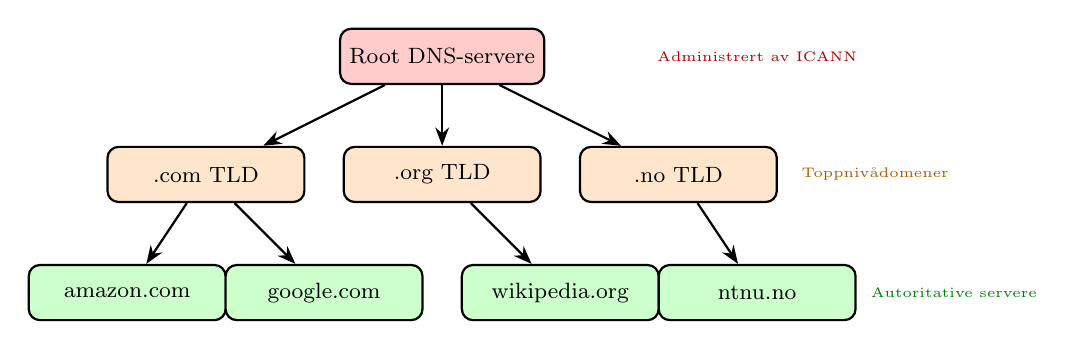
\begin{tikzpicture}[
    dns/.style={rectangle, draw, rounded corners, minimum width=2.5cm, minimum height=0.7cm, font=\footnotesize},
    >=Stealth, thick
]
    \node[dns, fill=red!20] (root) at (0,3) {Root DNS-servere};
    \node[dns, fill=orange!20] (tld1) at (-3,1.5) {.com TLD};
    \node[dns, fill=orange!20] (tld2) at (0,1.5) {.org TLD};
    \node[dns, fill=orange!20] (tld3) at (3,1.5) {.no TLD};
    \node[dns, fill=green!20] (auth1) at (-4,0) {amazon.com};
    \node[dns, fill=green!20] (auth2) at (-1.5,0) {google.com};
    \node[dns, fill=green!20] (auth3) at (1.5,0) {wikipedia.org};
    \node[dns, fill=green!20] (auth4) at (4,0) {ntnu.no};

    \draw[->] (root) -- (tld1);
    \draw[->] (root) -- (tld2);
    \draw[->] (root) -- (tld3);
    \draw[->] (tld1) -- (auth1);
    \draw[->] (tld1) -- (auth2);
    \draw[->] (tld2) -- (auth3);
    \draw[->] (tld3) -- (auth4);

    % Labels
    \node[font=\tiny, text=red!70!black] at (4,3) {Administrert av ICANN};
    \node[font=\tiny, text=orange!70!black] at (5.5,1.5) {Toppniv\aa domener};
    \node[font=\tiny, text=green!50!black] at (6.5,0) {Autoritative servere};
\end{tikzpicture}
\end{center}

\begin{keybox}[DNS-servertyper]
\begin{itemize}[noitemsep]
    \item \textbf{Root}: siste instans n\aa r andre servere ikke kan l\o se; administrert av ICANN
    \item \textbf{TLD (Top-Level Domain)}: h\aa ndterer .com, .org, .net, landdomener (.no)
    \item \textbf{Autoritativ}: gir offisielle hostname$\rightarrow$IP-mappinger for en organisasjon
    \item \textbf{Lokal DNS-server}: ikke del av hierarkiet; f\o rste stopp for DNS-sp\o rringer, svarer fra cache eller videresender
\end{itemize}
\end{keybox}

\subsection{DNS-sp\o rringer: Iterativ vs. Rekursiv}

\begin{center}
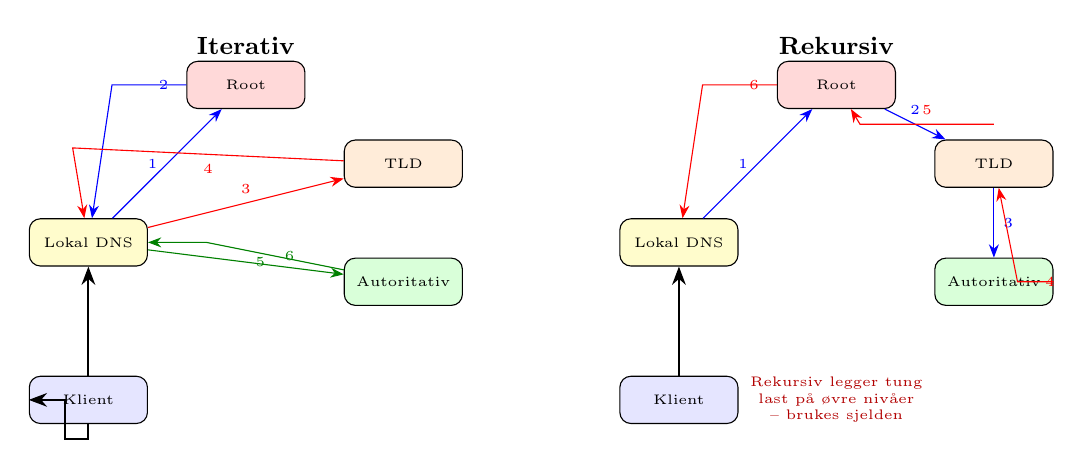
\begin{tikzpicture}[
    dns/.style={rectangle, draw, rounded corners, fill=blue!10, minimum width=1.5cm, minimum height=0.6cm, font=\tiny},
    >=Stealth
]
    % Iterative
    \node[font=\bfseries\small] at (-3.5,4.5) {Iterativ};
    \node[dns] (host1) at (-5.5,0) {Klient};
    \node[dns, fill=yellow!20] (local1) at (-5.5,2) {Lokal DNS};
    \node[dns, fill=red!15] (root1) at (-3.5,4) {Root};
    \node[dns, fill=orange!15] (tld1r) at (-1.5,3) {TLD};
    \node[dns, fill=green!15] (auth1r) at (-1.5,1.5) {Autoritativ};

    \draw[->, thick] (host1) -- (local1);
    \draw[->, blue] (local1) -- (root1) node[midway, left, font=\tiny] {1};
    \draw[<-, blue] (local1) -- ++(0.3,2) -- (root1) node[midway, right, font=\tiny] {2};
    \draw[->, red] (local1) -- (tld1r) node[midway, above, font=\tiny] {3};
    \draw[<-, red] (local1) -- ++(-0.2,1.2) -- (tld1r) node[midway, below, font=\tiny] {4};
    \draw[->, green!50!black] (local1) -- (auth1r) node[midway, right, font=\tiny] {5};
    \draw[<-, green!50!black] (local1) -- ++(1.5,0) -- (auth1r) node[midway, right, font=\tiny] {6};
    \draw[<-, thick] (host1) -- ++(-0.3,0) -- ++(0,-0.5) -- ++(0.3,0) -- (host1);

    % Recursive
    \node[font=\bfseries\small] at (4,4.5) {Rekursiv};
    \node[dns] (host2) at (2,0) {Klient};
    \node[dns, fill=yellow!20] (local2) at (2,2) {Lokal DNS};
    \node[dns, fill=red!15] (root2) at (4,4) {Root};
    \node[dns, fill=orange!15] (tld2r) at (6,3) {TLD};
    \node[dns, fill=green!15] (auth2r) at (6,1.5) {Autoritativ};

    \draw[->, thick] (host2) -- (local2);
    \draw[->, blue] (local2) -- (root2) node[midway, left, font=\tiny] {1};
    \draw[->, blue] (root2) -- (tld2r) node[midway, above, font=\tiny] {2};
    \draw[->, blue] (tld2r) -- (auth2r) node[midway, right, font=\tiny] {3};
    \draw[<-, red] (tld2r) -- ++(0.3,-1.5) -- (auth2r) node[midway, right, font=\tiny] {4};
    \draw[<-, red] (root2) -- ++(0.3,-0.5) -- ++(1.7,0) node[midway, above, font=\tiny] {5};
    \draw[<-, red] (local2) -- ++(0.3,2) -- (root2) node[midway, right, font=\tiny] {6};

    \node[font=\tiny, text=red!70!black, align=center] at (4,0) {Rekursiv legger tung\\last p\aa\ \o vre niv\aa er\\-- brukes sjelden};
\end{tikzpicture}
\end{center}

\subsection{DNS-caching og records}

\begin{keybox}[DNS Caching]
\begin{itemize}[noitemsep]
    \item Servere \textbf{cacher} svar for \aa\ f\aa\ raskere oppslag
    \item Oppf\o ringer har en \textbf{TTL} (Time To Live) -- utl\o per etter en viss tid
    \item Ulempe: cachede oppf\o ringer kan v\ae re \textbf{utdaterte} f\o r TTL utl\o per
\end{itemize}
\end{keybox}

\begin{keybox}[DNS Resource Records (RR)]
Format: \texttt{(name, value, type, TTL)}

\begin{tabular}{llll}
\toprule
\textbf{Type} & \textbf{Name} & \textbf{Value} & \textbf{Beskrivelse} \\
\midrule
\textbf{A} & hostname & IP-adresse & Direkte mapping \\
\textbf{NS} & domene & hostname for DNS-server & Navneserver \\
\textbf{CNAME} & alias & kanonisk navn & Alias \\
\textbf{MX} & domene & mailserver-hostname & Mailserver \\
\bottomrule
\end{tabular}
\end{keybox}

\begin{keybox}[DNS-sikkerhet]
\begin{itemize}[noitemsep]
    \item DDoS-beskyttelse: trafikkfiltrering, caching i lokale DNS-servere
    \item \textbf{DNSSEC}: autentisering og meldingsintegritet
\end{itemize}
\end{keybox}

%--- Exam questions 2.4 ---
\begin{exambox}[Eksamenssp\o rsm\aa l -- 2.4 DNS]
\small
\begin{longtable}{p{7cm}p{7cm}}
\toprule
\textbf{Sp\o rsm\aa l} & \textbf{Svar} \\
\midrule
\endhead
What does DNS stand for and what is its main role? & Domain Name System; translates hostnames to IP addresses. \\
\midrule
How is DNS implemented? & As a distributed, hierarchical database with many name servers. \\
\midrule
List the hierarchy of DNS servers. & Root $\rightarrow$ TLD $\rightarrow$ Authoritative $\rightarrow$ Local DNS server. \\
\midrule
What are TLD servers responsible for? & Managing top-level domains like .com, .org, .net, and country domains. \\
\midrule
What do authoritative DNS servers do? & They provide the official hostname-to-IP mappings for an organization. \\
\midrule
Explain iterated DNS query. & The contacted server replies with the next server to ask, not the final answer. \\
\midrule
Explain recursive DNS query. & The contacted server handles the full resolution and replies with the answer. \\
\midrule
What types of DNS records exist? & A (IP address), NS (name server), CNAME (alias), MX (mail server). \\
\midrule
How does caching improve DNS? & By storing mappings to speed up responses and reduce traffic. \\
\midrule
What protocol provides DNS security? & DNSSEC, which authenticates and ensures message integrity. \\
\bottomrule
\end{longtable}
\end{exambox}


\newpage
%=============================================================================
\section{P2P-fildistribusjon (2.5)}
%=============================================================================

\subsection{Client-Server vs. P2P distribusjon}

\begin{keybox}[Distribusjonstid -- Kjernesp\o rsm\aa let]
Hvor lang tid tar det \aa\ distribuere en fil (st\o rrelse $F$) fra \textit{en} server til $N$ peers?

Variabler:
\begin{itemize}[noitemsep]
    \item $u_s$ = serverens upload-kapasitet
    \item $d_i$ = peer $i$s download-kapasitet
    \item $u_i$ = peer $i$s upload-kapasitet
    \item $d_{\min}$ = minste download-rate blant alle peers
\end{itemize}
\end{keybox}

\begin{formulabox}[Client-Server distribusjonstid]
$$D_{CS} \geq \max\left\{\frac{NF}{u_s},\ \frac{F}{d_{\min}}\right\}$$
\begin{itemize}[noitemsep]
    \item $NF/u_s$: serveren m\aa\ sende $N$ kopier sekvensielt
    \item $F/d_{\min}$: tregeste klient bestemmer minimumstiden
    \item \textbf{\O ker line\ae rt med $N$}
\end{itemize}
\end{formulabox}

\begin{formulabox}[P2P distribusjonstid]
$$D_{P2P} \geq \max\left\{\frac{F}{u_s},\ \frac{F}{d_{\min}},\ \frac{NF}{u_s + \sum u_i}\right\}$$
\begin{itemize}[noitemsep]
    \item $F/u_s$: serveren m\aa\ laste opp \textit{minst} en kopi
    \item $F/d_{\min}$: tregeste klient kan ikke f\aa\ filen raskere
    \item $NF/(u_s + \sum u_i)$: total last deles av \textbf{alle} upload-kapasiteter
    \item \textbf{Selvskaler\-ende}: $\sum u_i$ vokser med $N$!
\end{itemize}
\end{formulabox}

\begin{center}
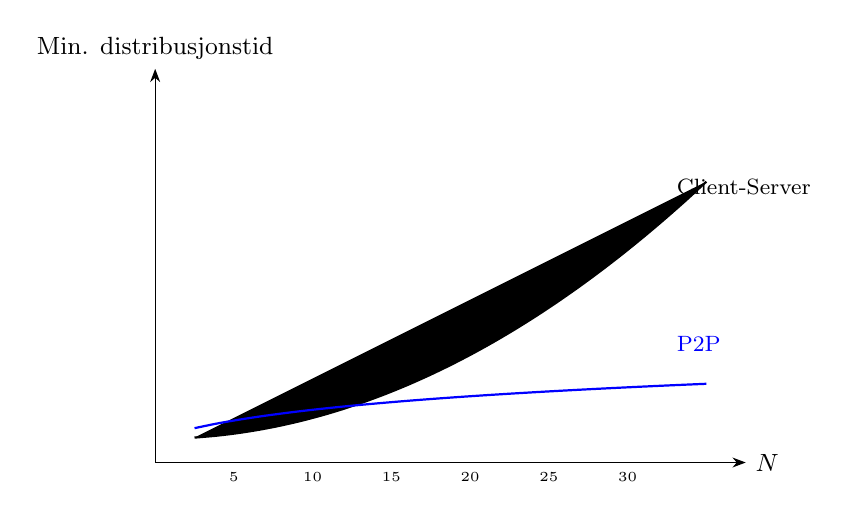
\begin{tikzpicture}[>=Stealth]
    % Axes
    \draw[->] (0,0) -- (7.5,0) node[right, font=\small] {$N$};
    \draw[->] (0,0) -- (0,5) node[above, font=\small] {Min. distribusjonstid};

    % Client-server (linear growth)
    \draw[thick, black, fill=black] plot[smooth, domain=0.5:7] (\x, {0.1*\x*\x/1.5 + 0.3});
    \node[font=\footnotesize, right] at (6.5,3.5) {Client-Server};

    % P2P (sub-linear, flattens)
    \draw[thick, blue] plot[smooth, domain=0.5:7] (\x, {0.3 + 0.7*ln(\x+1)/ln(8)});
    \node[font=\footnotesize, right, text=blue] at (6.5,1.5) {P2P};

    % Labels
    \foreach \x in {5,10,15,20,25,30} {
        \pgfmathsetmacro{\pos}{\x/5}
        \node[font=\tiny, below] at (\pos,0) {\x};
    }
\end{tikzpicture}
\end{center}

\begin{warnbox}[{Eksempel: $u_s = 10u$, $F/u = 1$ time, $d_{\min} \geq u_s$}]
\textbf{Client-Server:} $D_{CS} = NF/u_s = NF/(10u) = N/10$ (line\ae rt)\\
\textbf{P2P:} $D_{P2P} = NF/(u_s + Nu) = NF/((10+N)u) = N/(10+N)$ (flater ut!)

N\aa r $N=30$: CS tar $3$ timer, P2P tar $0.75$ timer.
\end{warnbox}

%--- Exam questions 2.5 ---
\begin{exambox}[Eksamenssp\o rsm\aa l -- 2.5 P2P]
\small
\begin{longtable}{p{7cm}p{7cm}}
\toprule
\textbf{Sp\o rsm\aa l} & \textbf{Svar} \\
\midrule
\endhead
What is the main difference between P2P and client-server? & P2P relies on direct peer communication; client-server depends on always-on servers. \\
\midrule
What is a major drawback of client-server file distribution? & Server must send a full copy to each peer, overloading it. \\
\midrule
How does P2P reduce server load? & Peers redistribute parts of the file they have received. \\
\midrule
What makes P2P self-scalable? & As more peers join, they also contribute upload bandwidth. \\
\midrule
What is the most popular P2P protocol (2020)? & BitTorrent. \\
\midrule
List key differences between CS and P2P distribution. & CS: server sends full file to each peer. P2P: peers share parts, reducing server load and increasing scalability. \\
\bottomrule
\end{longtable}
\end{exambox}


\newpage
%=============================================================================
\section{Videostreaming og CDN (2.6)}
%=============================================================================

\subsection{Multimedia: Video}

\begin{keybox}[Video og koding]
\begin{itemize}[noitemsep]
    \item Video = sekvens av bilder vist med konstant rate (f.eks. 24 fps)
    \item Digitalt bilde = array av piksler, hver representert med bits
    \item \textbf{Koding} utnytter redundans for \aa\ redusere bits:
    \begin{itemize}[noitemsep]
        \item \textbf{Spatial koding}: redundans \textit{innenfor} ett bilde (f.eks. mange like piksler)
        \item \textbf{Temporal koding}: redundans \textit{mellom} bilder (send bare forskjeller)
    \end{itemize}
\end{itemize}
\end{keybox}

\begin{keybox}[CBR vs. VBR]
\begin{tabular}{lll}
\toprule
& \textbf{CBR} & \textbf{VBR} \\
\midrule
Full form & Constant Bit Rate & Variable Bit Rate \\
Koding & Fast rate & Rate endres med innhold \\
\bottomrule
\end{tabular}

\vspace{0.3em}
Eksempler: MPEG1 (1.5 Mbps), MPEG2 (3--6 Mbps), MPEG4 (64 Kbps -- 12 Mbps)
\end{keybox}

\subsection{Streaming av lagret video}

\begin{center}
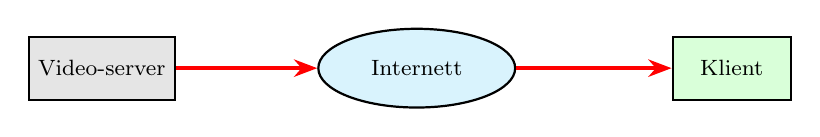
\begin{tikzpicture}[
    box/.style={rectangle, draw, fill=blue!10, minimum width=1.5cm, minimum height=0.8cm, font=\footnotesize},
    >=Stealth, thick
]
    \node[box, fill=gray!20] (server) at (0,0) {Video-\\server};
    \node[ellipse, draw, fill=cyan!15, minimum width=2.5cm, minimum height=1cm, font=\footnotesize] (inet) at (4,0) {Internett};
    \node[box, fill=green!15] (client) at (8,0) {Klient};

    \draw[->, red, very thick] (server) -- (inet);
    \draw[->, red, very thick] (inet) -- (client);
\end{tikzpicture}
\end{center}

\textbf{Utfordringer:}
\begin{itemize}[noitemsep]
    \item B\aa ndbredde varierer over tid (congestion)
    \item Pakketap og forsinkelse gir d\aa rlig kvalitet
\end{itemize}

\begin{warnbox}[Continuous Playout Constraint]
N\aa r avspilling starter, m\aa\ den matche original timing. Men nettverksforsinkelser varierer (\textbf{jitter}), s\aa\ klienten trenger en \textbf{buffer} og \textbf{playout delay} for \aa\ kompensere.
\end{warnbox}

\subsection{DASH -- Dynamic Adaptive Streaming over HTTP}

\begin{keybox}[DASH]
\textbf{Server:}
\begin{itemize}[noitemsep]
    \item Deler video i \textbf{chunks} (segmenter)
    \item Hvert chunk kodet i \textbf{flere kvalitetsniv\aa er} (bitrater)
    \item \textbf{Manifest-fil}: liste over URLer for ulike chunks/kvaliteter
\end{itemize}

\textbf{Klient (``intelligence'' at client):}
\begin{itemize}[noitemsep]
    \item M\aa ler server-til-klient b\aa ndbredde periodisk
    \item Bestemmer \textbf{n\aa r} chunk skal hentes (unng\aa\ buffer starvation/overflow)
    \item Bestemmer \textbf{hvilken bitrate} (h\o yere kvalitet n\aa r mer b\aa ndbredde)
    \item Bestemmer \textbf{hvor} chunk hentes fra (n\ae rmeste server)
\end{itemize}

\textbf{Streaming video = koding + DASH + playout buffering}
\end{keybox}

\subsection{CDN -- Content Distribution Networks}

\begin{warnbox}[Hvorfor ikke en mega-server?]
\begin{itemize}[noitemsep]
    \item Single point of failure
    \item Flaskehals for trafikk (congestion)
    \item Lang avstand til fjerne klienter
    \item Flere kopier av video over samme link
    \item \textbf{L\o sningen skalerer ikke!}
\end{itemize}
\end{warnbox}

\begin{keybox}[CDN -- To strategier]
\textbf{``Enter Deep'':}
\begin{itemize}[noitemsep]
    \item Plasser CDN-servere \textbf{dypt inne} i aksessnettverk, n\ae r brukerne
    \item Mange sm\aa\ serverklynger
\end{itemize}

\textbf{``Bring Home'':}
\begin{itemize}[noitemsep]
    \item F\ae rre, \textbf{st\o rre} CDN-klynger n\ae r aksessnettverk (ikke inne i dem)
\end{itemize}

Klienten f\aa r manifest fra CDN, henter chunks fra \textbf{best egnet server} med passende bitrate.
\end{keybox}

\begin{center}
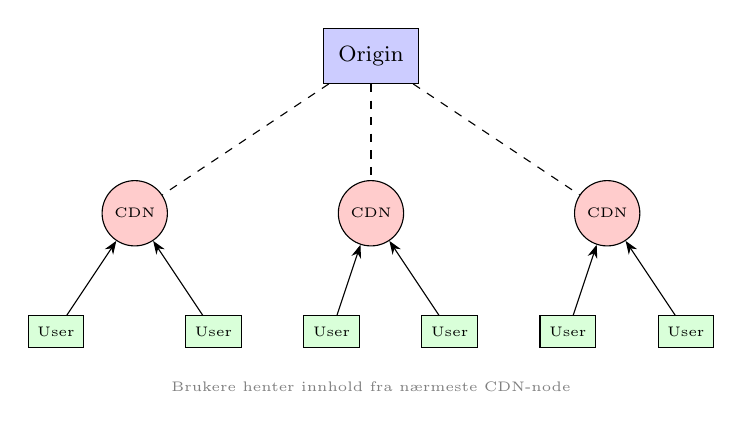
\begin{tikzpicture}[
    cdn/.style={circle, draw, fill=red!20, minimum size=0.7cm, font=\tiny},
    user/.style={rectangle, draw, fill=green!15, minimum width=0.6cm, minimum height=0.4cm, font=\tiny},
    >=Stealth
]
    % Origin
    \node[rectangle, draw, fill=blue!20, minimum width=1.2cm, minimum height=0.7cm, font=\footnotesize] (origin) at (0,2) {Origin};

    % CDN nodes
    \node[cdn] (cdn1) at (-3,0) {CDN};
    \node[cdn] (cdn2) at (0,0) {CDN};
    \node[cdn] (cdn3) at (3,0) {CDN};

    % Users
    \node[user] (u1) at (-4,-1.5) {User};
    \node[user] (u2) at (-2,-1.5) {User};
    \node[user] (u3) at (-0.5,-1.5) {User};
    \node[user] (u4) at (1,-1.5) {User};
    \node[user] (u5) at (2.5,-1.5) {User};
    \node[user] (u6) at (4,-1.5) {User};

    \draw[dashed] (origin) -- (cdn1);
    \draw[dashed] (origin) -- (cdn2);
    \draw[dashed] (origin) -- (cdn3);
    \draw[->] (u1) -- (cdn1);
    \draw[->] (u2) -- (cdn1);
    \draw[->] (u3) -- (cdn2);
    \draw[->] (u4) -- (cdn2);
    \draw[->] (u5) -- (cdn3);
    \draw[->] (u6) -- (cdn3);

    \node[font=\tiny, text=gray] at (0,-2.2) {Brukere henter innhold fra n\ae rmeste CDN-node};
\end{tikzpicture}
\end{center}

\begin{keybox}[OTT -- Over-the-Top]
Tjenester som Netflix, YouTube kj\o rer ``over'' den eksisterende IP-infrastrukturen. De kontrollerer ikke nettverket, men bruker CDN-er for \aa\ levere innhold effektivt.
\end{keybox}

%--- Exam questions 2.6 ---
\begin{exambox}[Eksamenssp\o rsm\aa l -- 2.6 Video og CDN]
\small
\begin{longtable}{p{7cm}p{7cm}}
\toprule
\textbf{Sp\o rsm\aa l} & \textbf{Svar} \\
\midrule
\endhead
How much of ISP traffic is video streaming? & About 80\%. \\
\midrule
What is spatial and temporal coding? & Spatial: within one image. Temporal: between images. \\
\midrule
What is DASH? & Dynamic Adaptive Streaming over HTTP. \\
\midrule
What does the server do in DASH? & Splits video into chunks, multiple qualities, provides manifest file. \\
\midrule
What does the client control in DASH? & When, which bitrate, and from where to request chunks. \\
\midrule
What is a CDN? & Content Delivery Network -- stores videos near users. \\
\midrule
Why not use one mega-server? & Bottleneck, single point of failure, long distance, doesn't scale. \\
\midrule
What is the ``Enter Deep'' strategy? & Place CDN servers deep inside access networks, close to users. \\
\midrule
What is the ``Bring Home'' strategy? & Fewer, larger CDN clusters near access networks. \\
\midrule
What is an OTT service? & Over-the-top service (e.g. Netflix), runs on top of IP infrastructure. \\
\bottomrule
\end{longtable}
\end{exambox}


\newpage
%=============================================================================
\section{Socket-programmering (2.7)}
%=============================================================================

\subsection{Grunnleggende om sockets}

\begin{keybox}[Socket = ``D\o ren'' mellom applikasjon og transport]
To typer sockets for to transporttjenester:
\begin{itemize}[noitemsep]
    \item \textbf{UDP socket}: up\aa litelig datagram (\texttt{SOCK\_DGRAM})
    \item \textbf{TCP socket}: p\aa litelig, byte stream-orientert (\texttt{SOCK\_STREAM})
\end{itemize}
\end{keybox}

\subsection{Socket-programmering med UDP}

\begin{keybox}[UDP -- Ingen tilkobling]
\begin{itemize}[noitemsep]
    \item \textbf{Ingen handshaking} f\o r dataoverf\o ring
    \item Sender legger til \textbf{IP-adresse og portnummer} til hvert pakke
    \item Mottaker henter senderens IP og port fra pakken
    \item Data kan g\aa\ \textbf{tapt} eller komme i \textbf{feil rekkef\o lge}
\end{itemize}
\end{keybox}

\begin{center}
\begin{tikzpicture}[
    step/.style={rectangle, draw, rounded corners, fill=blue!10, minimum width=4cm, minimum height=0.5cm, font=\tiny, align=center},
    >=Stealth, thick
]
    % Server side
    \node[font=\small\bfseries] at (-3,5) {Server};
    \node[step, fill=orange!15] (s1) at (-3,4) {Opprett socket\\(AF\_INET, SOCK\_DGRAM)};
    \node[step, fill=orange!15] (s2) at (-3,2.8) {bind() til port};
    \node[step, fill=orange!15] (s3) at (-3,1.5) {recvfrom() -- les datagram};
    \node[step, fill=orange!15] (s4) at (-3,0.2) {sendto() -- svar med\\klientadresse};

    \draw[->] (s1) -- (s2);
    \draw[->] (s2) -- (s3);
    \draw[->] (s3) -- (s4);

    % Client side
    \node[font=\small\bfseries] at (3,5) {Klient};
    \node[step, fill=green!15] (c1) at (3,4) {Opprett socket\\(AF\_INET, SOCK\_DGRAM)};
    \node[step, fill=green!15] (c2) at (3,2.8) {sendto() -- send med\\server IP + port};
    \node[step, fill=green!15] (c3) at (3,1.5) {recvfrom() -- les svar};
    \node[step, fill=green!15] (c4) at (3,0.2) {close()};

    \draw[->] (c1) -- (c2);
    \draw[->] (c2) -- (c3);
    \draw[->] (c3) -- (c4);

    % Communication arrows
    \draw[->, red, dashed, thick] (c2.west) -- (s3.east) node[midway, above, font=\tiny] {datagram};
    \draw[->, red, dashed, thick] (s4.east) -- (c3.west) node[midway, below, font=\tiny] {svar};
\end{tikzpicture}
\end{center}

\textbf{Python UDP-klient:}
\begin{lstlisting}
from socket import *
serverName = 'hostname'
serverPort = 12000
clientSocket = socket(AF_INET, SOCK_DGRAM)
message = input('Input lowercase sentence:')
clientSocket.sendto(message.encode(), (serverName, serverPort))
modifiedMessage, serverAddress = clientSocket.recvfrom(2048)
print(modifiedMessage.decode())
clientSocket.close()
\end{lstlisting}

\textbf{Python UDP-server:}
\begin{lstlisting}
from socket import *
serverPort = 12000
serverSocket = socket(AF_INET, SOCK_DGRAM)
serverSocket.bind(('', serverPort))
print("The server is ready to receive")
while True:
    message, clientAddress = serverSocket.recvfrom(2048)
    modifiedMessage = message.decode().upper()
    serverSocket.sendto(modifiedMessage.encode(), clientAddress)
\end{lstlisting}

\subsection{Socket-programmering med TCP}

\begin{keybox}[TCP -- Tilkoblingsorientert]
\begin{itemize}[noitemsep]
    \item Serveren m\aa\ kj\o re f\o rst og ha opprettet en \textbf{``welcoming socket''}
    \item Klienten oppretter TCP-socket med serverens IP + port $\rightarrow$ \textbf{TCP-tilkobling} opprettes
    \item Serveren oppretter \textbf{ny socket} (\texttt{connectionSocket}) for hver klient
    \item Bruker \textbf{source port} for \aa\ skille klienter
    \item TCP gir p\aa litelig, ordnet \textbf{byte-stream} overf\o ring
\end{itemize}
\end{keybox}

\begin{center}
\begin{tikzpicture}[
    step/.style={rectangle, draw, rounded corners, fill=blue!10, minimum width=4cm, minimum height=0.5cm, font=\tiny, align=center},
    >=Stealth, thick
]
    % Server side
    \node[font=\small\bfseries] at (-3,6.5) {Server};
    \node[step, fill=orange!15] (s1) at (-3,5.7) {Opprett socket\\(AF\_INET, SOCK\_STREAM)};
    \node[step, fill=orange!15] (s2) at (-3,4.5) {bind() + listen()};
    \node[step, fill=orange!15] (s3) at (-3,3.3) {connectionSocket =\\accept()};
    \node[step, fill=orange!15] (s4) at (-3,2) {recv() -- les data};
    \node[step, fill=orange!15] (s5) at (-3,0.8) {send() -- send svar};
    \node[step, fill=orange!15] (s6) at (-3,-0.3) {close() connectionSocket};

    \draw[->] (s1) -- (s2);
    \draw[->] (s2) -- (s3);
    \draw[->] (s3) -- (s4);
    \draw[->] (s4) -- (s5);
    \draw[->] (s5) -- (s6);

    % Client side
    \node[font=\small\bfseries] at (3,6.5) {Klient};
    \node[step, fill=green!15] (c1) at (3,5.7) {Opprett socket\\(AF\_INET, SOCK\_STREAM)};
    \node[step, fill=green!15] (c2) at (3,4.5) {connect() til server\\IP + port};
    \node[step, fill=green!15] (c3) at (3,3.3) {send() -- send data};
    \node[step, fill=green!15] (c4) at (3,2) {recv() -- les svar};
    \node[step, fill=green!15] (c5) at (3,0.8) {close()};

    \draw[->] (c1) -- (c2);
    \draw[->] (c2) -- (c3);
    \draw[->] (c3) -- (c4);
    \draw[->] (c4) -- (c5);

    % TCP connection
    \draw[<->, blue, dashed, very thick] (c2.west) -- (s3.east) node[midway, above, font=\tiny\bfseries] {TCP connection setup};
    \draw[->, red, dashed] (c3.west) -- (s4.east);
    \draw[->, red, dashed] (s5.east) -- (c4.west);
\end{tikzpicture}
\end{center}

\textbf{Python TCP-klient:}
\begin{lstlisting}
from socket import *
serverName = 'servername'
serverPort = 12000
clientSocket = socket(AF_INET, SOCK_STREAM)
clientSocket.connect((serverName, serverPort))
sentence = input('Input lowercase sentence:')
clientSocket.send(sentence.encode())
modifiedSentence = clientSocket.recv(1024)
print('From Server:', modifiedSentence.decode())
clientSocket.close()
\end{lstlisting}

\textbf{Python TCP-server:}
\begin{lstlisting}
from socket import *
serverPort = 12000
serverSocket = socket(AF_INET, SOCK_STREAM)
serverSocket.bind(('', serverPort))
serverSocket.listen(1)
print('The server is ready to receive')
while True:
    connectionSocket, addr = serverSocket.accept()
    sentence = connectionSocket.recv(1024).decode()
    capitalizedSentence = sentence.upper()
    connectionSocket.send(capitalizedSentence.encode())
    connectionSocket.close()
\end{lstlisting}

\subsection{Viktige forskjeller: UDP vs. TCP sockets}

\begin{keybox}[Sammenligning UDP vs. TCP]
\begin{tabular}{lll}
\toprule
\textbf{Egenskap} & \textbf{UDP} & \textbf{TCP} \\
\midrule
Socket-type & \texttt{SOCK\_DGRAM} & \texttt{SOCK\_STREAM} \\
Tilkobling & Ingen & Connection setup \\
P\aa litelighet & Up\aa litelig & P\aa litelig, ordnet \\
Dataenhet & Datagram (pakke) & Byte stream \\
Adressering & Eksplisitt per pakke & Automatisk (via connect) \\
Send-metode & \texttt{sendto()} & \texttt{send()} \\
Motta-metode & \texttt{recvfrom()} & \texttt{recv()} \\
Server ny socket? & Nei & Ja (\texttt{accept()}) \\
\bottomrule
\end{tabular}
\end{keybox}

%--- Exam questions 2.7 ---
\begin{exambox}[Eksamenssp\o rsm\aa l -- 2.7 Socket-programmering]
\small
\begin{longtable}{p{7cm}p{7cm}}
\toprule
\textbf{Sp\o rsm\aa l} & \textbf{Svar} \\
\midrule
\endhead
What is a socket? & A door between an application process and the end-end transport protocol. \\
\midrule
What are the two types of sockets? & UDP: unreliable datagram. TCP: reliable, byte stream-oriented. \\
\midrule
How does the client send data in UDP? & It attaches IP address and port number to each packet. \\
\midrule
What must happen before a TCP client contacts the server? & The server must be running and have created a welcoming socket. \\
\midrule
Why does the server create a new socket for each client in TCP? & To allow communication with multiple clients simultaneously. \\
\midrule
What does TCP use to distinguish different clients? & Source port numbers. \\
\midrule
What does TCP provide from the app's view? & Reliable, in-order byte-stream transfer between client and server. \\
\midrule
Why might an app choose UDP over TCP? & When low overhead and speed are more important than reliability. \\
\midrule
Why might an app choose TCP over UDP? & When reliable and ordered delivery of data is needed. \\
\bottomrule
\end{longtable}
\end{exambox}


\newpage
%=============================================================================
\section{Oppsummering -- Kapittel 2}
%=============================================================================

\begin{keybox}[Kapittel 2: Hovedtemaer]
\begin{itemize}[noitemsep]
    \item \textbf{Applikasjonsarkitekturer}: klient-server og P2P
    \item \textbf{Tjenestekrav}: p\aa litelighet, b\aa ndbredde, forsinkelse
    \item \textbf{Transportmodell}: TCP (p\aa litelig, tilkoblingsorientert) vs. UDP (up\aa litelig, datagram)
    \item \textbf{Protokoller}: HTTP, SMTP, IMAP, DNS, BitTorrent
    \item \textbf{Videostreaming}: DASH, CDN
    \item \textbf{Socket-programmering}: TCP og UDP sockets i Python
\end{itemize}
\end{keybox}

\begin{keybox}[Viktige temaer \aa\ forst\aa]
\begin{itemize}[noitemsep]
    \item \textbf{Sentralisert vs. desentralisert} (DNS, CDN, P2P)
    \item \textbf{Stateless vs. stateful} (HTTP er stateless, cookies gir tilstand)
    \item \textbf{Skalerbarhet} (P2P vs. client-server distribusjonstid)
    \item \textbf{P\aa litelig vs. up\aa litelig} meldingsoverf\o ring (TCP vs. UDP)
    \item \textbf{``Complexity at the network edge''} -- intelligens i endepunktene
\end{itemize}
\end{keybox}

\begin{formulabox}[Formelsammendrag]
\textbf{Non-persistent HTTP responstid:}
$$T = 2 \cdot RTT + T_{\text{fil}}$$

\textbf{Client-Server distribusjonstid:}
$$D_{CS} \geq \max\left\{\frac{NF}{u_s},\ \frac{F}{d_{\min}}\right\}$$

\textbf{P2P distribusjonstid:}
$$D_{P2P} \geq \max\left\{\frac{F}{u_s},\ \frac{F}{d_{\min}},\ \frac{NF}{u_s + \sum u_i}\right\}$$
\end{formulabox}

\begin{keybox}[Portnumre \aa\ huske]
\begin{tabular}{ll}
\toprule
\textbf{Protokoll} & \textbf{Port} \\
\midrule
HTTP & 80 \\
HTTPS & 443 \\
SMTP & 25 \\
DNS & 53 \\
\bottomrule
\end{tabular}
\end{keybox}


% ============================================================
%  CHAPTER 3
% ============================================================
\chapterdivider{3}{Chapter 3: The Transport Layer}
\section{Transportlagstjenester og protokoller (3.1)}
%=============================================================================

\subsection{Transportlagets rolle}

\begin{keybox}[Transportlaget -- oversikt]
Transportlaget tilbyr \textbf{logisk kommunikasjon} mellom \emph{applikasjonsprosesser} p\aa\ forskjellige verter (hosts).
\begin{itemize}[noitemsep]
    \item Sendersiden: bryter applikasjonsmeldinger i \textbf{segmenter}, sender dem til nettverkslaget
    \item Mottakersiden: setter segmenter sammen til meldinger, leverer til applikasjonslaget
    \item To hovedprotokoller: \textbf{TCP} og \textbf{UDP}
\end{itemize}
\end{keybox}

\subsection{Transportlag vs. nettverkslag}

\begin{keybox}[Viktig forskjell]
\begin{itemize}[noitemsep]
    \item \textbf{Nettverkslag (IP):} Logisk kommunikasjon mellom \emph{verter} (hosts)
    \item \textbf{Transportlag (TCP/UDP):} Logisk kommunikasjon mellom \emph{prosesser}
    \item Transportlaget utvider nettverkslagets host-til-host-levering til prosess-til-prosess-levering
\end{itemize}
\end{keybox}

\begin{warnbox}[Husholdningsanalogi]
Tenk p\aa\ to hus med 12 barn i hvert hus som sender brev til hverandre:
\begin{itemize}[noitemsep]
    \item \textbf{Prosesser} = barn
    \item \textbf{Applikasjonsmeldinger} = brev i konvolutter
    \item \textbf{Verter (hosts)} = hus
    \item \textbf{Transportprotokoll} = Ann og Bill (barna som samler/sorterer post)
    \item \textbf{Nettverkslagsprotokoll} = postvesenet
\end{itemize}
Ann og Bill jobber innenfor huset -- de kan ikke kontrollere hva som skjer ute i postsystemet.
\end{warnbox}

\subsection{Internettets transportprotokoller}

\begin{keybox}[TCP vs. UDP -- oversikt]
\textbf{TCP (Transmission Control Protocol):}
\begin{itemize}[noitemsep]
    \item P\aa litelig, ordnet levering (\emph{reliable, in-order delivery})
    \item Metningskontroll (\emph{congestion control})
    \item Flytkontroll (\emph{flow control})
    \item Tilkoblingssoppsett (\emph{connection setup})
\end{itemize}

\textbf{UDP (User Datagram Protocol):}
\begin{itemize}[noitemsep]
    \item Up\aa litelig, uordnet levering (\emph{unreliable, unordered delivery})
    \item Ingen metningskontroll, flytkontroll eller tilkoblingsoppsett
    \item ``Best effort'' -- ingen garanti p\aa\ levering
\end{itemize}

\textbf{Tjenester som IKKE tilbys:} Forsinkelses- eller b\aa ndbreddegarantier.
\end{keybox}

%=============================================================================
\section{Multipleksing og demultipleksing (3.2)}
%=============================================================================

\subsection{Grunnleggende konsept}

\begin{keybox}[Multipleksing og demultipleksing]
\textbf{Multipleksing hos sender:}
\begin{itemize}[noitemsep]
    \item H\aa ndterer data fra flere sokler (sockets)
    \item Legger til transportheader (med portnummer) for \aa\ identifisere sokkel
\end{itemize}

\textbf{Demultipleksing hos mottaker:}
\begin{itemize}[noitemsep]
    \item Bruker headerinformasjon (portnummer) for \aa\ levere segmenter til riktig sokkel
\end{itemize}
\end{keybox}

\subsection{Hvordan demultipleksing fungerer}

\begin{itemize}[noitemsep]
    \item Verten mottar IP-datagrammer -- hvert datagram har kilde-IP, destinasjons-IP og ett transportlags-segment
    \item Hvert segment har \textbf{kilde-portnummer} og \textbf{destinasjons-portnummer} (16 bit hver)
    \item Verten bruker IP-adresser og portnumre for \aa\ dirigere segmentet til riktig sokkel
\end{itemize}

\begin{center}
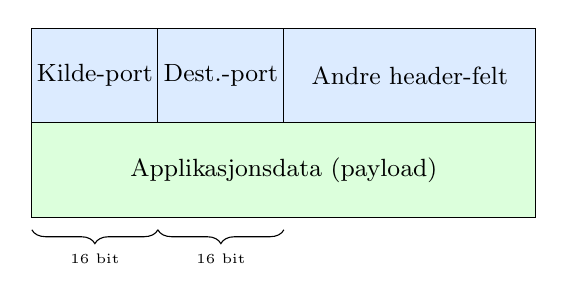
\begin{tikzpicture}[scale=0.8]
    \draw[fill=lightblue] (0,0) rectangle (8,1.5);
    \draw (2,0) -- (2,1.5);
    \draw (4,0) -- (4,1.5);
    \node at (1,0.75) {\small Kilde-port};
    \node at (3,0.75) {\small Dest.-port};
    \node at (6,0.75) {\small Andre header-felt};
    \draw[fill=lightgreen] (0,-1.5) rectangle (8,0);
    \node at (4,-0.75) {\small Applikasjonsdata (payload)};
    \draw[decorate,decoration={brace,amplitude=5pt,mirror}] (0,-1.7) -- (2,-1.7) node[midway,below=5pt]{\tiny 16 bit};
    \draw[decorate,decoration={brace,amplitude=5pt,mirror}] (2,-1.7) -- (4,-1.7) node[midway,below=5pt]{\tiny 16 bit};
\end{tikzpicture}
\end{center}

\subsection{Tilkoblingsl\o s demultipleksing (UDP)}

\begin{keybox}[UDP-sokkel identifiseres av 2-tuppel]
UDP-sokkel identifiseres av: \textbf{(destinasjons-IP, destinasjons-port)}
\begin{itemize}[noitemsep]
    \item Segmenter med \emph{samme} destinasjons-IP og destinasjons-port, men \emph{forskjellig} kilde-IP/port, dirigeres til \textbf{samme sokkel}
    \item Kilde-port brukes som ``returadresse''
\end{itemize}
\end{keybox}

\subsection{Tilkoblingsorientert demultipleksing (TCP)}

\begin{keybox}[TCP-sokkel identifiseres av 4-tuppel]
TCP-sokkel identifiseres av: \textbf{(kilde-IP, kilde-port, destinasjons-IP, destinasjons-port)}
\begin{itemize}[noitemsep]
    \item Mottaker bruker \emph{alle fire verdier} for \aa\ dirigere segmentet til riktig sokkel
    \item Serververten kan st\o tte mange samtidige TCP-sokler -- hver identifisert med sin egen 4-tuppel
    \item Webservere har ulike sokler for hver klient (ulik kilde-IP og/eller kilde-port)
\end{itemize}
\end{keybox}

\begin{warnbox}[Viktig forskjell UDP vs. TCP demux]
\begin{itemize}[noitemsep]
    \item \textbf{UDP:} Kun destinasjons-port avgj\o r hvilken sokkel som f\aa r segmentet
    \item \textbf{TCP:} B\aa de kilde og destinasjon (IP + port) avgj\o r sokkel -- to klienter med ulik kilde-IP/port f\aa r \emph{separate} sokler
\end{itemize}
\end{warnbox}

%=============================================================================
\section{Tilkoblingsl\o s transport: UDP (3.3)}
%=============================================================================

\subsection{UDP -- oversikt}

\begin{keybox}[UDP -- User Datagram Protocol (RFC 768)]
\begin{itemize}[noitemsep]
    \item ``Bare bein'' transportprotokoll -- ``no frills''
    \item \textbf{Best effort}: Segmenter kan g\aa\ tapt eller leveres i feil rekkef\o lge
    \item \textbf{Tilkoblingsl\o s:} Ingen h\aa ndtrykk mellom sender og mottaker, hvert segment h\aa ndteres uavhengig
\end{itemize}

\textbf{Hvorfor brukes UDP?}
\begin{itemize}[noitemsep]
    \item Ingen tilkoblingsoppsett (som gir forsinkelse)
    \item Enkel: ingen tilstand i sender/mottaker
    \item Liten header (8 byte vs. 20 byte for TCP)
    \item Ingen metningskontroll -- kan sende s\aa\ raskt som \o nsket / applikasjonen tillater
\end{itemize}
\end{keybox}

\subsection{Bruksomr\aa der for UDP}

\begin{itemize}[noitemsep]
    \item Streaming av multimedia (tolererer tap, hastighetssensitiv)
    \item DNS (raske, korte foresp\o rsler)
    \item SNMP (nettverksadministrasjon)
    \item HTTP/3 (bruker QUIC over UDP)
\end{itemize}

\begin{warnbox}[UDP og p\aa litelighet]
Hvis p\aa litelig overf\o ring er n\o dvendig over UDP, m\aa\ det legges til i \textbf{applikasjonslaget}. Eksempel: HTTP/3 / QUIC legger til p\aa litelighet og metningskontroll over UDP.
\end{warnbox}

\subsection{UDP-segmentformat}

\begin{center}
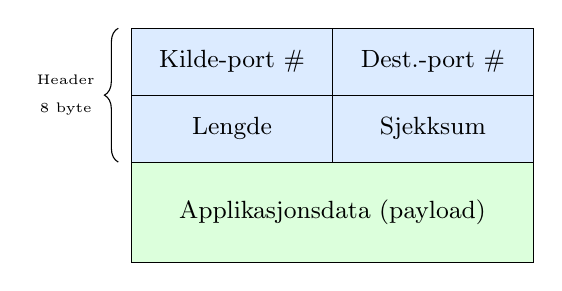
\begin{tikzpicture}[scale=0.85]
    \draw[fill=lightblue] (0,2) rectangle (3,3);
    \draw[fill=lightblue] (3,2) rectangle (6,3);
    \node at (1.5,2.5) {\small Kilde-port \#};
    \node at (4.5,2.5) {\small Dest.-port \#};

    \draw[fill=lightblue] (0,1) rectangle (3,2);
    \draw[fill=lightblue] (3,1) rectangle (6,2);
    \node at (1.5,1.5) {\small Lengde};
    \node at (4.5,1.5) {\small Sjekksum};

    \draw[fill=lightgreen] (0,-0.5) rectangle (6,1);
    \node at (3,0.25) {\small Applikasjonsdata (payload)};

    \draw[decorate,decoration={brace,amplitude=5pt}] (-0.2,1) -- (-0.2,3) node[midway,left=5pt,align=center]{\tiny Header\\[-2pt]\tiny 8 byte};
\end{tikzpicture}
\end{center}

\subsection{UDP sjekksum (checksum)}

\begin{keybox}[Sjekksum -- feildeteksjon]
\textbf{M\aa l:} Oppdage ``feil'' (f.eks. flippede biter) i det overf\o rte segmentet.

\textbf{Sender:}
\begin{itemize}[noitemsep]
    \item Behandler segmentinnholdet (inkludert header-felt) som en sekvens av 16-biters ord
    \item Legger sammen alle 16-biters ord med \textbf{1-er-komplement-addisjon}
    \item Tar \textbf{1-er-komplementet} av resultatet = sjekksum
    \item Plasserer sjekksummen i UDP-headerens sjekksumfelt
\end{itemize}

\textbf{Mottaker:}
\begin{itemize}[noitemsep]
    \item Beregner sjekksummen av mottatt segment (inkludert sjekksumfeltet)
    \item Hvis resultatet \emph{ikke} er \texttt{1111111111111111} $\Rightarrow$ feil detektert
    \item Hvis resultatet er alle 1-ere $\Rightarrow$ ingen feil detektert (men det kan fortsatt v\ae re feil!)
\end{itemize}
\end{keybox}

\begin{formulabox}[Sjekksum-eksempel]
Legg sammen to 16-biters ord:
\begin{align*}
&\texttt{1110011001100110} \\
+\ &\texttt{1101010101010101} \\
=\ &\texttt{1011101110111011} \quad \text{(med wraparound carry)} \\
\text{Sjekksum} =\ &\texttt{0100010001000100} \quad \text{(1-er-komplement)}
\end{align*}
\end{formulabox}

%=============================================================================
\section{Prinsipper for p\aa litelig dataoverf\o ring (3.4)}
%=============================================================================

\subsection{Problemstilling}

P\aa litelig dataoverf\o ring er et av de viktigste problemene i nettverking. Utfordringen er \aa\ bygge en \textbf{p\aa litelig kanal} over en \textbf{up\aa litelig kanal} (som kan miste pakker, flippe biter, osv.).

\begin{center}
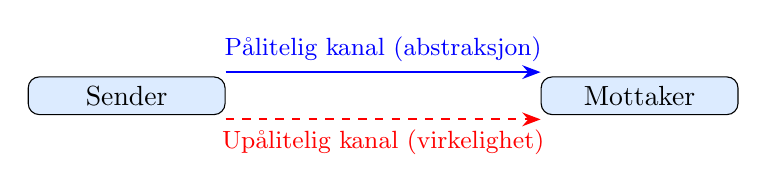
\begin{tikzpicture}[>=Stealth, node distance=2.5cm]
    \node[draw, rounded corners, fill=lightblue, minimum width=2.5cm] (s) {Sender};
    \node[draw, rounded corners, fill=lightblue, minimum width=2.5cm, right=4cm of s] (r) {Mottaker};
    \draw[->, thick, blue] ([yshift=3mm]s.east) -- ([yshift=3mm]r.west) node[midway, above]{\small P\aa litelig kanal (abstraksjon)};
    \draw[->, thick, red, dashed] ([yshift=-3mm]s.east) -- ([yshift=-3mm]r.west) node[midway, below]{\small Up\aa litelig kanal (virkelighet)};
\end{tikzpicture}
\end{center}

\subsection{rdt1.0: Overf\o ring over perfekt p\aa litelig kanal}

\begin{keybox}[rdt1.0 -- Enkleste tilfellet]
\textbf{Antagelse:} Underliggende kanal er \emph{perfekt p\aa litelig} (ingen bitfeil, ingen pakketap).

\textbf{Sender:} Bare send data ned i kanalen.\\
\textbf{Mottaker:} Bare les data fra kanalen.

Ingen feilh\aa ndtering n\o dvendig -- trivielt!
\end{keybox}

\subsection{rdt2.0: Kanal med bitfeil}

\begin{keybox}[rdt2.0 -- Stopp-og-vent med ACK/NAK]
\textbf{Antagelse:} Kanalen kan ha \emph{bitfeil} (men ingen pakketap).

\textbf{Nye mekanismer:}
\begin{itemize}[noitemsep]
    \item \textbf{Sjekksum:} Oppdager bitfeil
    \item \textbf{ACK (acknowledgement):} Mottaker sier ``OK, mottatt korrekt''
    \item \textbf{NAK (negative acknowledgement):} Mottaker sier ``feil, send p\aa\ nytt''
    \item \textbf{Retransmisjon:} Sender retransmitterer ved NAK
\end{itemize}
Senderen sender \'{e}n pakke og \textbf{venter} p\aa\ ACK/NAK f\o r neste pakke sendes (\emph{stop-and-wait}).
\end{keybox}

\begin{warnbox}[Fatalt problem med rdt2.0!]
Hva hvis ACK/NAK selv har bitfeil? Senderen vet ikke om pakken ble mottatt korrekt!
\begin{itemize}[noitemsep]
    \item Kan ikke bare retransmittere -- gir mulige duplikater
    \item L\o sning $\rightarrow$ rdt2.1
\end{itemize}
\end{warnbox}

\subsection{rdt2.1: Sekvensnumre}

\begin{keybox}[rdt2.1 -- L\o sning: Sekvensnumre]
Sender legger til et \textbf{sekvensnummer} (0 eller 1) p\aa\ hver pakke:
\begin{itemize}[noitemsep]
    \item Hvis ACK/NAK er korrupt $\rightarrow$ sender retransmitterer gjeldende pakke
    \item Mottaker forkaster duplikater ved hjelp av sekvensnummeret
    \item To sekvensnumre (0 og 1) er tilstrekkelig for stopp-og-vent
\end{itemize}
\end{keybox}

\subsection{rdt2.2: NAK-fri protokoll}

\begin{keybox}[rdt2.2 -- Kun ACK (ingen NAK)]
Samme funksjonalitet som rdt2.1, men \emph{uten NAK}:
\begin{itemize}[noitemsep]
    \item Mottaker sender \textbf{ACK med sekvensnummeret} til siste korrekt mottatte pakke
    \item Duplikat-ACK hos sender fungerer som NAK (betyr: ``den siste pakken var feil'')
    \item Sender retransmitterer n\aa r den f\aa r duplikat-ACK
\end{itemize}
\end{keybox}

\subsection{rdt3.0: Kanal med bitfeil OG pakketap}

\begin{keybox}[rdt3.0 -- Timer / Countdown timer]
\textbf{Ny antagelse:} Kanalen kan ogs\aa\ \emph{miste pakker} (data eller ACKer).

\textbf{Ny mekanisme: Nedtellingstimer (countdown timer)}
\begin{itemize}[noitemsep]
    \item Sender venter en ``rimelig'' tid p\aa\ ACK
    \item Retransmitterer hvis ingen ACK mottas innen timeout
    \item Hvis pakken (eller ACK) bare er forsinket (ikke tapt): retransmisjon gir duplikat, men sekvensnumre h\aa ndterer dette
\end{itemize}
rdt3.0 er korrekt, men ytelsen er d\aa rlig p\aa\ h\o ykapasitets-lenker!
\end{keybox}

\subsection{Ytelse til rdt3.0 (stopp-og-vent)}

\begin{formulabox}[Utnyttelsesgrad for stopp-og-vent]
\[
U_{\text{sender}} = \frac{L/R}{RTT + L/R}
\]
hvor:
\begin{itemize}[noitemsep]
    \item $L$ = pakkest\o rrelse (bits)
    \item $R$ = linkekapasitet (bps)
    \item $RTT$ = rundturstid (round-trip time)
    \item $L/R$ = overf\o ringstid for \'{e}n pakke
\end{itemize}
\end{formulabox}

\begin{exambox}[Eksempel: D\aa rlig utnyttelse]
Gitt: $L = 8000$ bits, $R = 1$ Gbps, $RTT = 30$ ms:
\[
U_{\text{sender}} = \frac{8000 / 10^9}{0{,}030 + 8000/10^9} = \frac{0{,}000008}{0{,}030008} = 0{,}00027 = 0{,}027\%
\]
Kun 0,027\% utnyttelse! Senderen er aktiv bare $0{,}008$ ms av $30{,}008$ ms.
\end{exambox}

\subsection{Pipelining: \o kt utnyttelse}

\begin{keybox}[Pipelining -- Send flere pakker uten \aa\ vente]
L\o sning p\aa\ d\aa rlig utnyttelse: \textbf{pipelining} -- sender tillater at flere pakker er ``in flight'' (sendt men ikke enda bekreftet).
\begin{itemize}[noitemsep]
    \item Krever st\o rre rekkevidde for sekvensnumre
    \item Buffering hos sender og/eller mottaker
    \item To hovedvarianter: \textbf{Go-Back-N} og \textbf{Selective Repeat}
\end{itemize}

\textbf{Med pipelining (3 pakker):}
\[
U_{\text{sender}} = \frac{3 \cdot L/R}{RTT + L/R}
\]
3x bedre utnyttelse enn stopp-og-vent!
\end{keybox}

\subsection{Go-Back-N (GBN)}

\begin{keybox}[Go-Back-N protokoll]
\textbf{Sender:}
\begin{itemize}[noitemsep]
    \item ``Vindu'' med opptil $N$ ubekreftede pakker i pipelinen
    \item \textbf{Kumulativ ACK:} ACK($n$) bekrefter alle pakker t.o.m. sekvensnummer $n$
    \item Timer for den eldste ubekreftede pakken
    \item Ved timeout: retransmitter \emph{alle} pakker i vinduet (fra eldste ubekreftede)
\end{itemize}

\textbf{Mottaker:}
\begin{itemize}[noitemsep]
    \item Sender kun ACK for h\o yeste korrekt mottatte pakke \emph{i rekkef\o lge}
    \item Kan ha kun \'{e}n forventet sekvensnummer
    \item Forkaster pakker som er ute av rekkef\o lge (ingen buffering) -- sender ACK p\aa\ nytt for siste i rekkef\o lge
\end{itemize}
\end{keybox}

\begin{center}
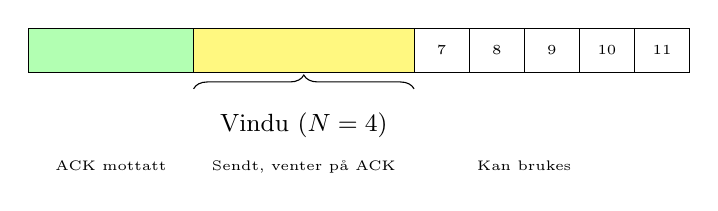
\begin{tikzpicture}[scale=0.7]
    \foreach \i in {0,...,11} {
        \draw (\i,0) rectangle (\i+1,0.8);
        \node at (\i+0.5,0.4) {\tiny \i};
    }
    \draw[fill=green!30] (0,0) rectangle (3,0.8);
    \draw[fill=yellow!50] (3,0) rectangle (7,0.8);

    \draw[decorate,decoration={brace,amplitude=5pt}] (3,-0.3) -- (7,-0.3) node[midway,below=5pt]{\small Vindu ($N=4$)};

    \node[below=1cm] at (1.5,0) {\tiny ACK mottatt};
    \node[below=1cm] at (5,0) {\tiny Sendt, venter p\aa\ ACK};
    \node[below=1cm] at (9,0) {\tiny Kan brukes};
\end{tikzpicture}
\end{center}

\subsection{Selective Repeat (SR)}

\begin{keybox}[Selective Repeat protokoll]
\textbf{Sender:}
\begin{itemize}[noitemsep]
    \item Vindu med opptil $N$ ubekreftede pakker
    \item \textbf{Individuell ACK:} Hver pakke har sin egen ACK
    \item Timer for \emph{hver} ubekreftet pakke
    \item Ved timeout: retransmitter kun den \emph{spesifikke} pakken som timet ut
\end{itemize}

\textbf{Mottaker:}
\begin{itemize}[noitemsep]
    \item Bekrefter \emph{hver} korrekt mottatt pakke individuelt
    \item \textbf{Bufferer} pakker mottatt ute av rekkef\o lge
    \item Leverer til applikasjonen n\aa r ``hullet'' fylles inn
\end{itemize}
\end{keybox}

\begin{warnbox}[SR-dilemmaet: Vindusst\o rrelse vs. sekvensnummerrom]
Vindusst\o rrelsen $N$ m\aa\ v\ae re \textbf{h\o yst halvparten av sekvensnummerrommet}:
\[
N \leq \frac{k}{2} \quad \text{der } k \text{ er antall mulige sekvensnumre}
\]
Ellers kan mottaker ikke skille mellom nye pakker og retransmisjoner!

\textbf{Eksempel:} Med sekvensnumre $\{0, 1, 2, 3\}$ (4 mulige) m\aa\ $N \leq 2$.
\end{warnbox}

\begin{center}
\begin{tabular}{lcc}
\toprule
\textbf{Egenskap} & \textbf{Go-Back-N} & \textbf{Selective Repeat} \\
\midrule
ACK-type & Kumulativ & Individuell \\
Mottaker-buffering & Nei & Ja \\
Ved timeout & Retransmitter alle & Retransmitter \'{e}n \\
Timer & \'{E}n (eldste) & Per pakke \\
Kompleksitet & Lavere & H\o yere \\
Effektivitet & Lavere (mange retransm.) & H\o yere \\
\bottomrule
\end{tabular}
\end{center}

%=============================================================================
\section{Tilkoblingsorientert transport: TCP (3.5)}
%=============================================================================

\subsection{TCP -- oversikt}

\begin{keybox}[TCP -- Egenskaper]
\begin{itemize}[noitemsep]
    \item \textbf{Punkt-til-punkt:} \'{E}n sender, \'{e}n mottaker
    \item \textbf{P\aa litelig, ordnet bytestr\o m:} Ingen meldingsgrenser
    \item \textbf{Full dupleks:} Data kan flyte begge veier samtidig (bi-directional data flow)
    \item \textbf{Kumulativ ACK}
    \item \textbf{Pipelining:} Vindusstyrte segmenter (congestion \& flow control setter vindu)
    \item \textbf{Tilkoblingsorientert:} H\aa ndtrykk (handshake) f\o r datautveksling
    \item \textbf{Flyt- og metningskontroll:} Sender overbelaster ikke mottaker eller nettverk
\end{itemize}
\end{keybox}

\subsection{TCP-segmentstruktur}

\begin{center}
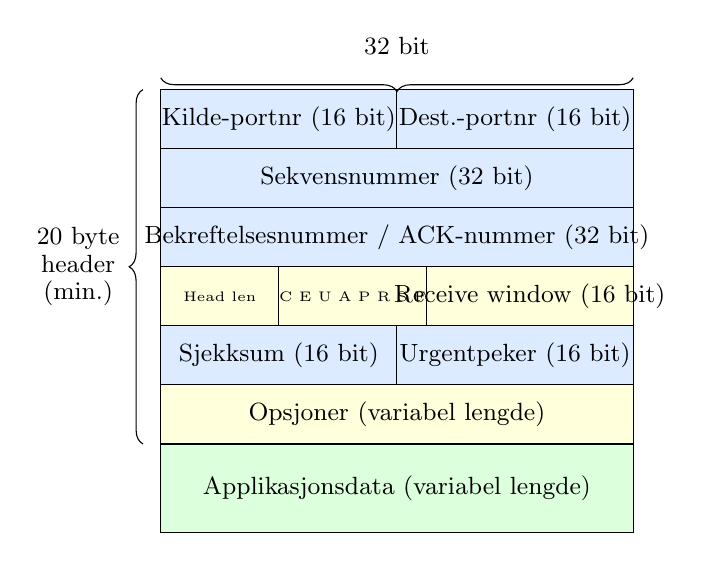
\begin{tikzpicture}[scale=0.75]
    % Row 1 - Source/Dest port
    \draw[fill=lightblue] (0,6) rectangle (4,7);
    \draw[fill=lightblue] (4,6) rectangle (8,7);
    \node at (2,6.5) {\small Kilde-portnr (16 bit)};
    \node at (6,6.5) {\small Dest.-portnr (16 bit)};

    % Row 2 - Sequence number
    \draw[fill=lightblue] (0,5) rectangle (8,6);
    \node at (4,5.5) {\small Sekvensnummer (32 bit)};

    % Row 3 - ACK number
    \draw[fill=lightblue] (0,4) rectangle (8,5);
    \node at (4,4.5) {\small Bekreftelsesnummer / ACK-nummer (32 bit)};

    % Row 4 - Header length, flags, receive window
    \draw[fill=lightyellow] (0,3) rectangle (2,4);
    \draw[fill=lightyellow] (2,3) rectangle (4.5,4);
    \draw[fill=lightyellow] (4.5,3) rectangle (8,4);
    \node at (1,3.5) {\tiny Head len};
    \node at (3.25,3.5) {\tiny C E U A P R S F};
    \node at (6.25,3.5) {\small Receive window (16 bit)};

    % Row 5 - Checksum, Urgent pointer
    \draw[fill=lightblue] (0,2) rectangle (4,3);
    \draw[fill=lightblue] (4,2) rectangle (8,3);
    \node at (2,2.5) {\small Sjekksum (16 bit)};
    \node at (6,2.5) {\small Urgentpeker (16 bit)};

    % Row 6 - Options
    \draw[fill=lightyellow] (0,1) rectangle (8,2);
    \node at (4,1.5) {\small Opsjoner (variabel lengde)};

    % Row 7 - Data
    \draw[fill=lightgreen] (0,-0.5) rectangle (8,1);
    \node at (4,0.25) {\small Applikasjonsdata (variabel lengde)};

    % Brace for header
    \draw[decorate,decoration={brace,amplitude=5pt}] (-0.3,1) -- (-0.3,7) node[midway,left=5pt,align=center]{\small 20 byte\\[-2pt]\small header\\[-2pt]\small (min.)};

    % Width annotation
    \draw[decorate,decoration={brace,amplitude=5pt,mirror}] (0,7.2) -- (8,7.2) node[midway,above=5pt]{\small 32 bit};
\end{tikzpicture}
\end{center}

\begin{keybox}[Viktige felt i TCP-headeren]
\begin{itemize}[noitemsep]
    \item \textbf{Sekvensnummer:} Bytenummer til f\o rste byte i segmentets data
    \item \textbf{ACK-nummer:} Neste byte mottakeren forventer (kumulativ ACK)
    \item \textbf{Receive window (rwnd):} Antall byte mottaker er villig til \aa\ akseptere (flytkontroll)
    \item \textbf{Flagg:} SYN, FIN, ACK, RST, PSH, URG, CWR, ECE
    \item \textbf{Header-lengde:} Variabel pga. opsjoner (normalt 20 byte uten opsjoner)
\end{itemize}
\end{keybox}

\subsection{MSS og MTU}

\begin{formulabox}[MSS og MTU]
\begin{itemize}[noitemsep]
    \item \textbf{MTU (Maximum Transmission Unit):} St\o rste linklags-ramme (typisk \textbf{1500 byte} for Ethernet)
    \item \textbf{MSS (Maximum Segment Size):} Maks applikasjonsdata i segment
    \item $\text{MSS} = \text{MTU} - \text{IP-header} - \text{TCP-header} = 1500 - 20 - 20 = \textbf{1460 byte}$
    \item MSS refererer til applikasjonsdata, \emph{ikke} inkludert TCP-header
\end{itemize}
\end{formulabox}

\subsection{TCP sekvensnumre og ACK}

\begin{keybox}[Sekvensnumre og ACK i TCP]
\textbf{Sekvensnumre:}
\begin{itemize}[noitemsep]
    \item TCP nummererer \emph{byte} (ikke segmenter!)
    \item Sekvensnummeret er bytenummeret til f\o rste databyte i segmentet
    \item Eksempel: fil p\aa\ 500\,000 byte, MSS = 1000 byte $\Rightarrow$ segment 0 har seq=0, segment 1 har seq=1000, segment 2 har seq=2000, \ldots
\end{itemize}

\textbf{ACK-numre:}
\begin{itemize}[noitemsep]
    \item ACK-nummeret er sekvensnummeret til \textbf{neste byte mottakeren forventer}
    \item \textbf{Kumulativ ACK:} Bekrefter alle byte t.o.m. ACK-nummer $-$ 1
    \item Sp\o rsm\aa l: Hva gj\o r mottaker med pakker ute av rekkef\o lge? TCP-spec sier ingenting -- opp til implementasjon (i praksis: buffer dem)
\end{itemize}
\end{keybox}

\begin{exambox}[Eksempel: Telnet-sesjon]
Vert A sender `C' (1 byte) til Vert B, begge starter med seq=42 (A) og seq=79 (B):
\begin{enumerate}[noitemsep]
    \item A $\rightarrow$ B: Seq=42, ACK=79, data=`C'
    \item B $\rightarrow$ A: Seq=79, ACK=43, data=`C' (ekko)
    \item A $\rightarrow$ B: Seq=43, ACK=80
\end{enumerate}
\end{exambox}

\subsection{TCP Round-Trip Time og timeout}

\begin{formulabox}[RTT-estimering og timeout]
\textbf{SampleRTT:} M\aa lt tid fra segment sendt til ACK mottatt (kun for segmenter sendt \'{e}n gang).

\textbf{Estimert RTT (eksponensielt vektet glidende gjennomsnitt -- EWMA):}
\[
\text{EstimatedRTT} = (1 - \alpha) \cdot \text{EstimatedRTT} + \alpha \cdot \text{SampleRTT}
\]
Typisk: $\alpha = 0{,}125$ (dvs. $1/8$)

\textbf{Avviksm\aa l (Safety margin):}
\[
\text{DevRTT} = (1 - \beta) \cdot \text{DevRTT} + \beta \cdot |\text{SampleRTT} - \text{EstimatedRTT}|
\]
Typisk: $\beta = 0{,}25$ (dvs. $1/4$)

\textbf{Timeout-intervall:}
\[
\text{TimeoutInterval} = \text{EstimatedRTT} + 4 \cdot \text{DevRTT}
\]
\end{formulabox}

\begin{warnbox}[Viktig om SampleRTT]
SampleRTT m\aa les \textbf{ikke} for retransmitterte segmenter (Karn's algoritme) -- man kan ikke vite om ACK-en er for originalen eller retransmisjonen.
\end{warnbox}

\subsection{TCP p\aa litelig dataoverf\o ring}

\begin{keybox}[TCP sender -- forenklet]
TCP bruker \textbf{\'{e}n retransmissjonstimer} per tilkobling (ikke per segment).

\textbf{Hendelser hos sender:}
\begin{enumerate}[noitemsep]
    \item \textbf{Data fra applikasjon:} Lag segment med sekvensnummer, start timer hvis ikke allerede kj\o rende
    \item \textbf{Timeout:} Retransmitter segmentet med lavest sekvensnummer som ikke er bekreftet. Start timer p\aa\ nytt
    \item \textbf{ACK mottatt:} Hvis ACK bekrefter tidligere ubekreftede segmenter -- oppdater hva som er bekreftet. Start timer p\aa\ nytt hvis det fortsatt er ubekreftede segmenter
\end{enumerate}
\end{keybox}

\begin{keybox}[TCP fast retransmit]
Hvis sender mottar \textbf{3 duplikat-ACKer} (dvs.\ 4 ACKer for samme segment): retransmitter segmentet \emph{f\o r timeout} utl\o per.

Rasjonale: Duplikat-ACKer indikerer at et segment har g\aa tt tapt, men etterfølgende segmenter har kommet frem.
\end{keybox}

\subsection{TCP flytkontroll}

\begin{keybox}[Flytkontroll -- Flow Control]
\textbf{M\aa l:} Sender skal ikke oversvjemme mottakers buffer.

\textbf{Mekanisme:}
\begin{itemize}[noitemsep]
    \item Mottaker annonserer ledig bufferplass i TCP-headeren via \textbf{rwnd}-feltet (receive window)
    \item $\text{rwnd} = \text{RcvBuffer} - (\text{LastByteRcvd} - \text{LastByteRead})$
    \item Sender begrenser ubekreftede data: $\text{LastByteSent} - \text{LastByteAcked} \leq \text{rwnd}$
    \item Standard RcvBuffer = 4096 byte (kan \o kes via operativsystem)
\end{itemize}
\end{keybox}

\begin{warnbox}[Hva n\aa r rwnd = 0?]
N\aa r mottaker annonserer $\text{rwnd} = 0$, sender sender fortsatt sm\aa\ \textbf{probe-segmenter} (1 byte) for \aa\ f\aa\ oppdatert rwnd-verdi og unng\aa\ deadlock.
\end{warnbox}

\subsection{TCP tilkoblingsadministrasjon}

\subsubsection{Treveis h\aa ndtrykk (3-way handshake)}

\begin{keybox}[TCP tilkoblingsoppsett -- 3-veis h\aa ndtrykk]
\begin{enumerate}[noitemsep]
    \item \textbf{SYN:} Klient sender SYN-segment (SYN=1, velger tilfeldig sekvensnummer \texttt{client\_isn})
    \item \textbf{SYN-ACK:} Server svarer med SYNACK (SYN=1, ACK=1, velger \texttt{server\_isn}, acker \texttt{client\_isn+1})
    \item \textbf{ACK:} Klient sender ACK (ACK=1, acker \texttt{server\_isn+1}). Kan inneholde data!
\end{enumerate}
\end{keybox}

\begin{center}
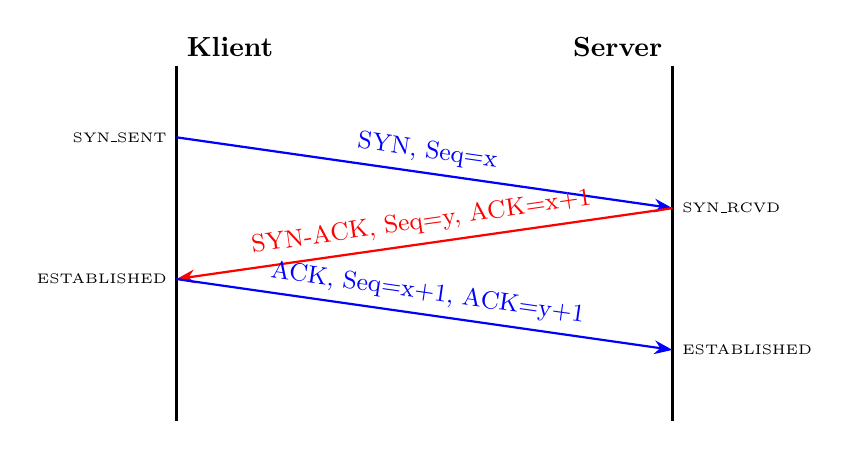
\begin{tikzpicture}[>=Stealth, scale=0.9]
    \draw[thick] (0,0) -- (0,-5) node[above right, at start]{\textbf{Klient}};
    \draw[thick] (7,0) -- (7,-5) node[above left, at start]{\textbf{Server}};

    \draw[->, blue, thick] (0,-1) -- (7,-2) node[midway, above, sloped]{\small SYN, Seq=x};
    \draw[->, red, thick] (7,-2) -- (0,-3) node[midway, above, sloped]{\small SYN-ACK, Seq=y, ACK=x+1};
    \draw[->, blue, thick] (0,-3) -- (7,-4) node[midway, above, sloped]{\small ACK, Seq=x+1, ACK=y+1};

    \node[left] at (0,-1) {\tiny SYN\_SENT};
    \node[right] at (7,-2) {\tiny SYN\_RCVD};
    \node[left] at (0,-3) {\tiny ESTABLISHED};
    \node[right] at (7,-4) {\tiny ESTABLISHED};
\end{tikzpicture}
\end{center}

\begin{warnbox}[Hvorfor ikke toveis h\aa ndtrykk?]
Et toveis h\aa ndtrykk feiler fordi:
\begin{itemize}[noitemsep]
    \item Variable forsinkelser -- retransmitterte meldinger kan ankomme etter at tilkoblingen er lukket
    \item Meldinger kan komme i feil rekkef\o lge
    \item Kan ikke ``se'' den andre siden -- \textbf{halvåpne tilkoblinger} oppst\aa r
\end{itemize}
\end{warnbox}

\subsubsection{Tilkoblingslukking}

\begin{keybox}[TCP tilkoblingslukking -- 4-stegs prosess]
\begin{enumerate}[noitemsep]
    \item Klient sender \textbf{FIN}-segment
    \item Server svarer med \textbf{ACK} (halvlukket -- server kan fortsatt sende data)
    \item Server sender \textbf{FIN}-segment
    \item Klient svarer med \textbf{ACK}, g\aa r inn i \textbf{TIME\_WAIT} (venter typisk 2 $\times$ MSL)
\end{enumerate}
\end{keybox}

\begin{center}
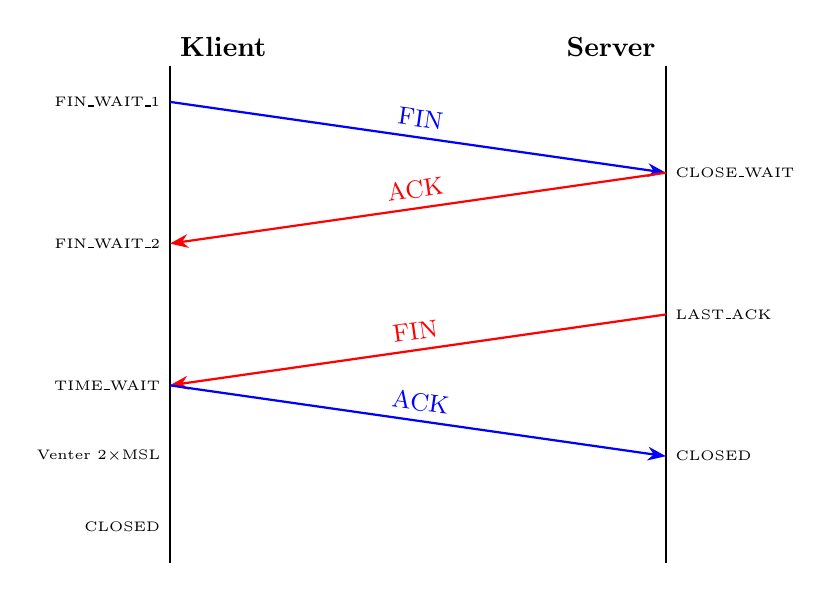
\begin{tikzpicture}[>=Stealth, scale=0.9]
    \draw[thick] (0,0) -- (0,-7) node[above right, at start]{\textbf{Klient}};
    \draw[thick] (7,0) -- (7,-7) node[above left, at start]{\textbf{Server}};

    \draw[->, blue, thick] (0,-0.5) -- (7,-1.5) node[midway, above, sloped]{\small FIN};
    \draw[->, red, thick] (7,-1.5) -- (0,-2.5) node[midway, above, sloped]{\small ACK};
    \draw[->, red, thick] (7,-3.5) -- (0,-4.5) node[midway, above, sloped]{\small FIN};
    \draw[->, blue, thick] (0,-4.5) -- (7,-5.5) node[midway, above, sloped]{\small ACK};

    \node[left] at (0,-0.5) {\tiny FIN\_WAIT\_1};
    \node[left] at (0,-2.5) {\tiny FIN\_WAIT\_2};
    \node[left] at (0,-4.5) {\tiny TIME\_WAIT};
    \node[right] at (7,-1.5) {\tiny CLOSE\_WAIT};
    \node[right] at (7,-3.5) {\tiny LAST\_ACK};
    \node[right] at (7,-5.5) {\tiny CLOSED};

    \draw[dashed] (0,-4.5) -- (0,-6.5) node[left, midway]{\tiny Venter 2$\times$MSL};
    \node[left] at (0,-6.5) {\tiny CLOSED};
\end{tikzpicture}
\end{center}

\subsubsection{TCP-tilstander}

\begin{center}
\begin{tabular}{ll}
\toprule
\textbf{Tilstand} & \textbf{Beskrivelse} \\
\midrule
CLOSED & Ingen tilkobling \\
LISTEN & Server venter p\aa\ innkommende SYN \\
SYN\_SENT & Klient har sendt SYN, venter p\aa\ SYN-ACK \\
SYN\_RCVD & Server har mottatt SYN, sendt SYN-ACK \\
ESTABLISHED & Tilkobling etablert, data kan overf\o res \\
FIN\_WAIT\_1 & Har sendt FIN, venter p\aa\ ACK \\
FIN\_WAIT\_2 & FIN bekreftet, venter p\aa\ FIN fra andre side \\
CLOSE\_WAIT & Mottatt FIN, venter p\aa\ at applikasjonen lukker \\
LAST\_ACK & Sendt FIN, venter p\aa\ siste ACK \\
TIME\_WAIT & Venter 2$\times$MSL f\o r \aa\ sikre at siste ACK mottas \\
\bottomrule
\end{tabular}
\end{center}

%=============================================================================
\section{Prinsipper for metningskontroll (3.6)}
%=============================================================================

\subsection{Hva er metning (congestion)?}

\begin{keybox}[Metning -- Congestion]
\textbf{Metning} oppst\aa r n\aa r for mange kilder sender for mye data for fort, slik at \textbf{nettverket} ikke klarer \aa\ h\aa ndtere alt.

\textbf{Symptomer:}
\begin{itemize}[noitemsep]
    \item Lange k\o forsinkelser (k\o er i ruterbuffere)
    \item Pakketap (buffer-overflyt i rutere)
\end{itemize}

\textbf{Forskjell fra flytkontroll:}
\begin{itemize}[noitemsep]
    \item \textbf{Flytkontroll:} Hindrer sender i \aa\ oversvjemme \emph{mottaker}
    \item \textbf{Metningskontroll:} Hindrer sender i \aa\ oversvjemme \emph{nettverket}
\end{itemize}
\end{keybox}

\subsection{Kostnader ved metning}

\begin{warnbox}[Kostnader ved metning]
\begin{itemize}[noitemsep]
    \item K\o forsinkelser \o ker n\aa r ankomsthastighet n\ae rmer seg linkkapasitet
    \item Retransmisjoner pga.\ pakketap -- ``wasted'' arbeid
    \item Un\o dvendige retransmisjoner (premature timeout) -- senderen sender \emph{kopier} av pakker som allerede er levert
    \item N\aa r en pakke droppes langs en sti, g\aa r all oppadg\aa ende overf\o ringskapasitet brukt p\aa\ den pakken til spille
\end{itemize}
\end{warnbox}

\subsection{Tilnm\ae rminger til metningskontroll}

\begin{keybox}[To hovedtilnm\ae rminger]
\textbf{1. End-to-end metningskontroll:}
\begin{itemize}[noitemsep]
    \item Ingen eksplisitt tilbakemelding fra nettverket
    \item Metning utledes fra observert tap og forsinkelse
    \item TCP bruker denne tilnm\ae rmingen
\end{itemize}

\textbf{2. Nettverksassistert metningskontroll:}
\begin{itemize}[noitemsep]
    \item Rutere gir tilbakemelding til sender
    \item Kan v\ae re \emph{direkte} (eksplisitt rate) eller \emph{indirekte} (ECN-bit i header)
    \item ECN (Explicit Congestion Notification): 2 bit i IP-headeren
\end{itemize}
\end{keybox}

%=============================================================================
\section{TCP metningskontroll (3.7)}
%=============================================================================

\subsection{Oversikt: CWND og RWND}

\begin{keybox}[De to ``bremsene'' i TCP]
TCP-sender begrenser overf\o ringshastigheten med to vinduer:
\begin{itemize}[noitemsep]
    \item \textbf{cwnd (Congestion Window):} Bestemt av \emph{senderen} basert p\aa\ observert metning. \emph{Ikke} synlig i headeren (intern variabel)
    \item \textbf{rwnd (Receive Window):} Bestemt av \emph{mottakeren}, annonsert i TCP-headeren
\end{itemize}

\textbf{Den gylne regel:}
\[
\text{LastByteSent} - \text{LastByteAcked} \leq \min(\text{cwnd}, \text{rwnd})
\]

\textbf{TCP senderate:}
\[
\text{rate} \approx \frac{\text{cwnd}}{\text{RTT}} \text{ bytes/sek}
\]
\end{keybox}

\begin{formulabox}[B\aa ndbredde med og uten metningskontroll]
\textbf{Uten} metningskontroll (pre-Tahoe):
\[
BW_i = \frac{\text{TCP Window}}{\text{RTT}} = \frac{\text{RWND} \cdot \text{MSS}}{\text{RTT}}
\]

\textbf{Med} metningskontroll:
\[
BW_i = \frac{\text{TCP Window}}{\text{RTT}} = \frac{\min(\text{CWND}, \text{RWND}) \cdot \text{MSS}}{\text{RTT}}
\]
\end{formulabox}

\subsection{TCP Slow Start}

\begin{keybox}[Slow Start -- Eksponentiell vekst]
Ved \textbf{tilkoblingsstart}:
\begin{itemize}[noitemsep]
    \item $\text{cwnd} = 1$ MSS
    \item Initial rate = MSS/RTT
    \item For \textbf{hver mottatt ACK}: $\text{cwnd} = \text{cwnd} + \text{MSS}$
    \item Resulterer i \textbf{dobling} av cwnd per RTT (eksponentiell vekst)
\end{itemize}

\textbf{Eksempel} (MSS = 500 bytes, RTT = 200 ms):\\
Initial rate = 500/0{,}2 = 20 kbps, men dobles for hver RTT.
\end{keybox}

\begin{exambox}[Slow Start beregning]
Om cwnd = 4500 og MSS = 1500:\\
Det sendes 4500/1500 = 3 segmenter, og det kommer 3 ACK denne RTT:
\begin{itemize}[noitemsep]
    \item ACK 1: cwnd = 4500 + 1500 = 6000
    \item ACK 2: cwnd = 6000 + 1500 = 7500
    \item ACK 3: cwnd = 7500 + 1500 = 9000
\end{itemize}
Dvs.\ cwnd \textbf{doblet} fra 4500 til 9000 p\aa\ \'{e}n RTT!
\end{exambox}

\subsection{Congestion Avoidance -- AIMD}

\begin{keybox}[Congestion Avoidance -- Line\ae r vekst]
N\aa r cwnd $\geq$ ssthresh (slow start threshold):
\begin{itemize}[noitemsep]
    \item \textbf{Additive Increase:} For hver mottatt ACK:
    \[
    \text{cwnd} = \text{cwnd} + \text{MSS} \cdot \frac{\text{MSS}}{\text{cwnd}}
    \]
    Resulterer i \o kning p\aa\ \textbf{1 MSS per RTT} (line\ae r vekst)
    \item \textbf{Multiplicative Decrease:} Ved pakketap: halver cwnd
\end{itemize}
Gir ``sagtann''-m\o nster (\emph{saw tooth behavior}) -- prober stadig etter ledig b\aa ndbredde.
\end{keybox}

\begin{exambox}[Congestion Avoidance beregning]
Om cwnd = 3000 og MSS = 1500 (i Congestion Avoidance):
\begin{itemize}[noitemsep]
    \item cwnd0 = 3000 (start av RTT)
    \item Det sendes 3000/1500 = 2 segmenter $\Rightarrow$ 2 ACK
    \item ACK 1: cwnd = 3000 + 1500$\cdot$(1500/3000) = 3000 + 750 = 3750
    \item ACK 2: cwnd = 3750 + 1500$\cdot$(1500/3750) = 3750 + 600 = 4350
\end{itemize}
Dvs.\ cwnd \o kte med ca.\ \textbf{1 MSS} til neste RTT (line\ae r vekst). (Eksakt 1 MSS ved start av neste RTT-periode.)
\end{exambox}

\subsection{Tapshendelser og ssthresh}

\begin{keybox}[Reaksjon p\aa\ tap -- ssthresh]
Variabelen \textbf{ssthresh} (slow start threshold) avgj\o r n\aa r man g\aa r fra Slow Start til Congestion Avoidance.

\textbf{Ved tapshendelse:}
\begin{itemize}[noitemsep]
    \item $\text{ssthresh} = \text{cwnd} / 2$
\end{itemize}

\textbf{To typer tap -- ulik respons:}

\textbf{1. Timeout:}
\begin{itemize}[noitemsep]
    \item ssthresh = cwnd/2
    \item cwnd = 1 MSS
    \item G\aa\ tilbake til \textbf{Slow Start}
\end{itemize}

\textbf{2. Trippel duplikat-ACK (3 dup ACK):}
\begin{itemize}[noitemsep]
    \item ssthresh = cwnd/2
    \item cwnd = ssthresh + 3 MSS
    \item G\aa\ inn i \textbf{Fast Recovery}
\end{itemize}
\end{keybox}

\subsection{De tre mekanismene i TCP metningskontroll}

\begin{center}
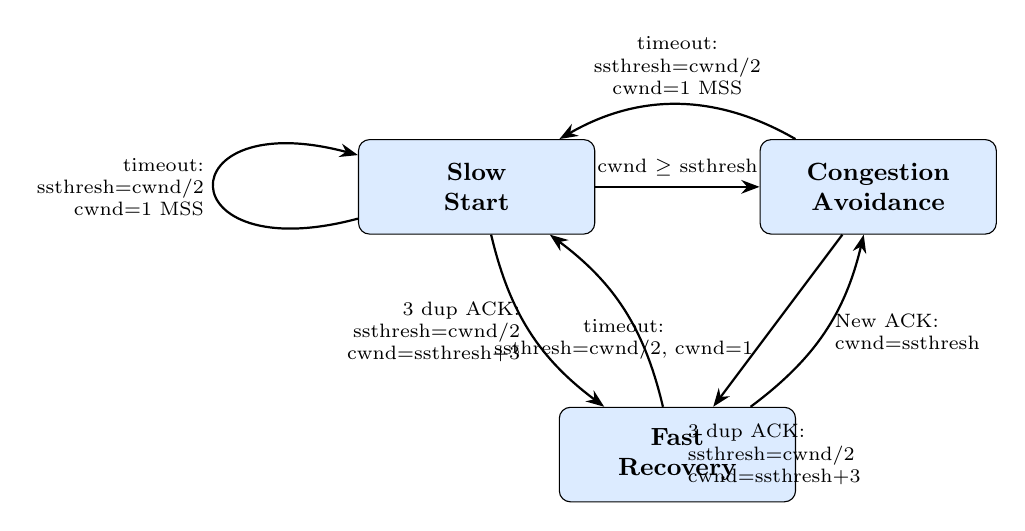
\begin{tikzpicture}[>=Stealth, scale=0.85,
    state/.style={draw, rounded corners, fill=lightblue, minimum width=3cm, minimum height=1.2cm, align=center, font=\small\bfseries}]

    \node[state] (ss) at (0,0) {Slow\\Start};
    \node[state] (ca) at (6,0) {Congestion\\Avoidance};
    \node[state] (fr) at (3,-4) {Fast\\Recovery};

    % SS -> CA
    \draw[->, thick] (ss) -- (ca) node[midway, above, font=\scriptsize]{cwnd $\geq$ ssthresh};

    % SS -> SS (timeout)
    \draw[->, thick] (ss) to[loop left] node[left, font=\scriptsize, align=right]{timeout:\\ssthresh=cwnd/2\\cwnd=1 MSS} (ss);

    % CA -> SS (timeout)
    \draw[->, thick] (ca) to[bend right=30] node[above, font=\scriptsize, align=center]{timeout:\\ssthresh=cwnd/2\\cwnd=1 MSS} (ss);

    % SS -> FR (3 dup ACK)
    \draw[->, thick] (ss) to[bend right=20] node[left, font=\scriptsize, align=right]{3 dup ACK:\\ssthresh=cwnd/2\\cwnd=ssthresh+3} (fr);

    % CA -> FR (3 dup ACK)
    \draw[->, thick] (ca) -- (fr) node[right, font=\scriptsize, align=left]{3 dup ACK:\\ssthresh=cwnd/2\\cwnd=ssthresh+3};

    % FR -> CA (new ACK)
    \draw[->, thick] (fr) to[bend right=20] node[right, font=\scriptsize, align=left]{New ACK:\\cwnd=ssthresh} (ca);

    % FR -> SS (timeout)
    \draw[->, thick] (fr) to[bend right=20] node[below, font=\scriptsize, align=center]{timeout:\\ssthresh=cwnd/2, cwnd=1} (ss);
\end{tikzpicture}
\end{center}

\subsection{TCP Tahoe vs. TCP Reno}

\begin{keybox}[TCP Tahoe vs. TCP Reno]
\textbf{TCP Tahoe (1988):}
\begin{itemize}[noitemsep]
    \item Ved \emph{alle} tapshendelser (b\aa de timeout og 3 dup ACK): cwnd = 1 MSS, g\aa\ til Slow Start
\end{itemize}

\textbf{TCP Reno (1997, RFC 2001/2581):}
\begin{itemize}[noitemsep]
    \item Ved \textbf{timeout}: cwnd = 1 MSS, g\aa\ til Slow Start (som Tahoe)
    \item Ved \textbf{3 dup ACK}: cwnd = ssthresh + 3, g\aa\ til Fast Recovery (mildere reaksjon)
    \item Fast Recovery gir bedre ytelse -- pakketap via dup-ACK betyr at nettverket fortsatt leverer noen pakker
\end{itemize}
\end{keybox}

\subsection{TCP CUBIC}

\begin{keybox}[TCP CUBIC -- Moderne metningskontroll]
TCP CUBIC er \textbf{standard i Linux} og den mest brukte TCP-varianten for webservere.

\textbf{Motivasjon:} Klassisk AIMD (line\ae r \o kning) er for treg n\aa r b\aa ndbredden er h\o y.

\textbf{Iid\'{e}:}
\begin{itemize}[noitemsep]
    \item $W_{\max}$ = senderate da metning sist ble oppdaget
    \item Etter halvering av cwnd: \o k raskt tilbake mot $W_{\max}$, men sakk ned n\ae r $W_{\max}$
    \item $K$ = tidspunkt da vinduet n\aa r $W_{\max}$ (konfigurerbar)
    \item \O kning av $W$ som funksjon av \textbf{kuben} av avstanden mellom n\aa v\ae rende tid og $K$
    \item St\o rre \o kninger n\aa r langt fra $K$, mindre \o kninger n\ae r $K$ (forsiktig)
\end{itemize}

\textbf{Fordeler:}
\begin{itemize}[noitemsep]
    \item Uavhengig av RTT (bruker veggklokketid)
    \item Rettferdig p\aa\ tvers av ulike RTT-er
    \item H\o yere gjennomstr\o mning enn klassisk TCP p\aa\ h\o yhastighetslenker
\end{itemize}
\end{keybox}

\subsection{TCP Fairness -- Rettferdighet}

\begin{keybox}[TCP Fairness]
\textbf{M\aa l:} Hvis $K$ TCP-sesjoner deler en flaskehalslenke med kapasitet $R$, b\o r hver f\aa\ gjennomsnittlig rate $R/K$.

\textbf{Hvorfor AIMD gir rettferdighet:}
\begin{itemize}[noitemsep]
    \item Additive Increase: begge sesjoner \o ker med stigning 1 (parallelt med likedelingslinjen)
    \item Multiplicative Decrease: begge halverer (beveger seg mot likedelingslinjen)
    \item Over tid konvergerer sesjonene mot lik andel av b\aa ndbredden
\end{itemize}

\textbf{NB:} Dette er et veldig teoretisk resultat -- i praksis p\aa virker RTT, antall tilkoblinger per applikasjon, og UDP-trafikk (som ikke har metningskontroll) rettferdigheten.
\end{keybox}

\subsection{Bottleneck-lenken}

\begin{warnbox}[Bottleneck-lenke og TCP-oppf\o rsel]
TCP (\aa de klassisk og CUBIC) \o ker senderaten til pakketap oppst\aa r ved en ruters utgang -- \textbf{bottleneck-lenken}.

\textbf{Viktige innsikter:}
\begin{itemize}[noitemsep]
    \item \O kt TCP-senderate \textbf{vil ikke} \o ke ende-til-ende-gjennomstr\o mning n\aa r bottleneck er mettet
    \item \O kt senderate \textbf{vil} \o ke m\aa lt RTT (pga. k\o er)
    \item M\aa l: ``Hold ende-til-ende-r\o ret akkurat fullt, men ikke fullere''
\end{itemize}
\end{warnbox}

%=============================================================================
\section{Evolusjon av transportlags-funksjonalitet (3.8)}
%=============================================================================

\subsection{Utfordringer med TCP}

\begin{keybox}[Ulike scenarier -- ulike utfordringer]
\begin{center}
\begin{tabular}{ll}
\toprule
\textbf{Scenario} & \textbf{Utfordring} \\
\midrule
Lange, fete r\o r (store dataoverf\o ringer) & Mange pakker ``in flight''; tap stopper pipeline \\
Tr\aa dl\o se nettverk & Tap pga.\ st\o y tolkes som metning \\
Lange forsinkelser & Ekstremt lang RTT \\
Datasenternettverk & Latens-sensitiv \\
Bakgrunnstrafikk & Lav-prioritets TCP-flyter \\
\bottomrule
\end{tabular}
\end{center}
\end{keybox}

\subsection{QUIC -- Quick UDP Internet Connections}

\begin{keybox}[QUIC og HTTP/3]
\textbf{QUIC} er en applikasjonslags-protokoll bygget \textbf{over UDP} som gir:
\begin{itemize}[noitemsep]
    \item P\aa litelig dataoverf\o ring
    \item Metningskontroll
    \item Autentisering og kryptering
    \item Tilkoblingsoppsett p\aa\ \textbf{1 RTT} (vs. TCP+TLS = 2 serielleh\aa ndtrykk)
\end{itemize}

\textbf{HTTP/3 = HTTP/2 (slanket) over QUIC over UDP}

\textbf{Fordeler over TCP:}
\begin{itemize}[noitemsep]
    \item Flere applikasjonsniv\aa\ ``str\o mmer'' multiplekset over \'{e}n QUIC-tilkobling
    \item Str\o mmene er \textbf{uavhengige} -- unng\aa r TCPs head-of-line blocking
    \item Separat p\aa litelig overf\o ring og sikkerhet per str\o m
    \item Felles metningskontroll p\aa\ tvers av str\o mmer
\end{itemize}
\end{keybox}

\begin{center}
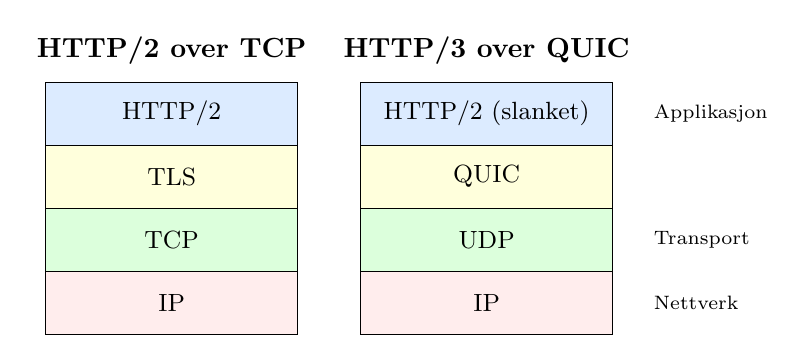
\begin{tikzpicture}[scale=0.8]
    % HTTP/2 over TCP stack
    \node at (2, 4.5) {\textbf{HTTP/2 over TCP}};
    \draw[fill=lightblue] (0,3) rectangle (4,4);
    \node at (2,3.5) {\small HTTP/2};
    \draw[fill=lightyellow] (0,2) rectangle (4,3);
    \node at (2,2.5) {\small TLS};
    \draw[fill=lightgreen] (0,1) rectangle (4,2);
    \node at (2,1.5) {\small TCP};
    \draw[fill=lightred!50] (0,0) rectangle (4,1);
    \node at (2,0.5) {\small IP};

    % HTTP/3 over QUIC stack
    \node at (7, 4.5) {\textbf{HTTP/3 over QUIC}};
    \draw[fill=lightblue] (5,3) rectangle (9,4);
    \node at (7,3.5) {\small HTTP/2 (slanket)};
    \draw[fill=lightyellow] (5,2) rectangle (9,3);
    \node at (7,2.5) {\small QUIC};
    \draw[fill=lightgreen] (5,1) rectangle (9,2);
    \node at (7,1.5) {\small UDP};
    \draw[fill=lightred!50] (5,0) rectangle (9,1);
    \node at (7,0.5) {\small IP};

    % Labels
    \node[right] at (9.5, 3.5) {\scriptsize Applikasjon};
    \node[right] at (9.5, 1.5) {\scriptsize Transport};
    \node[right] at (9.5, 0.5) {\scriptsize Nettverk};
\end{tikzpicture}
\end{center}

\subsection{TCPs historiske utvikling}

\begin{center}
\begin{tabular}{lll}
\toprule
\textbf{\AA r} & \textbf{Milepæl} & \textbf{Kommentar} \\
\midrule
1980--81 & RFC 761 / RFC 793 & Opprinnelig TCP (kun Connection + Transfer) \\
1988 & TCP Tahoe (BSD) & Jacobson: Slow Start + Congestion Avoidance \\
1997 & TCP Reno (RFC 2001/2581) & Fast Retransmit + Fast Recovery \\
2005 & BIC TCP & Binm\ae r s\o k etter optimal vindusstm\o rrelse \\
2018 & TCP CUBIC & Kubisk funksjon, standard i Linux \\
\bottomrule
\end{tabular}
\end{center}

%=============================================================================
\section{Oppsummering}
%=============================================================================

\begin{keybox}[Kapittel 3 -- Hovedpunkter]
\begin{itemize}[noitemsep]
    \item \textbf{Transportlaget} gir logisk kommunikasjon mellom \emph{prosesser} (ikke verter)
    \item \textbf{Multipleksing/demultipleksing:} Portnumre dirigerer til riktig sokkel (UDP: 2-tuppel, TCP: 4-tuppel)
    \item \textbf{UDP:} Enkel, tilkoblingsl\o s, ``best effort'' -- bare mux/demux + sjekksum
    \item \textbf{P\aa litelig dataoverf\o ring:} Sjekksum, sekvensnumre, ACK, timer, retransmisjon
    \item \textbf{Pipelining:} GBN (kumulativ ACK, retransmitter alle) vs. SR (individuell ACK, buffer ute-av-rekkef\o lge)
    \item \textbf{TCP:} P\aa litelig, ordnet bytestr\o m med flytkontroll, metningskontroll og tilkoblingsadministrasjon
    \item \textbf{TCP metningskontroll:} Slow Start (eksponentiell), Congestion Avoidance (AIMD), Fast Recovery
    \item \textbf{TCP CUBIC:} Kubisk vindusm\o kning, standard i Linux, RTT-uavhengig
    \item \textbf{QUIC/HTTP/3:} Moderne alternativ over UDP med 1-RTT tilkobling og uavhengige str\o mmer
\end{itemize}
\end{keybox}

%=============================================================================
\section*{Formelsammendrag}
%=============================================================================

\begin{formulabox}[Alle viktige formler -- Kapittel 3]

\textbf{UDP sjekksum:} 1-er-komplement av summen av alle 16-biters ord.

\textbf{Stopp-og-vent utnyttelse:}
\[
U_{\text{sender}} = \frac{L/R}{RTT + L/R}
\]

\textbf{Pipelining utnyttelse ($n$ pakker):}
\[
U_{\text{sender}} = \frac{n \cdot L/R}{RTT + L/R}
\]

\textbf{MSS:}
\[
\text{MSS} = \text{MTU} - \text{IP-header} - \text{TCP-header} = 1500 - 20 - 20 = 1460 \text{ byte}
\]

\textbf{RTT-estimering:}
\begin{align*}
\text{EstimatedRTT} &= (1 - \alpha) \cdot \text{EstimatedRTT} + \alpha \cdot \text{SampleRTT} & (\alpha = 0{,}125) \\
\text{DevRTT} &= (1 - \beta) \cdot \text{DevRTT} + \beta \cdot |\text{SampleRTT} - \text{EstimatedRTT}| & (\beta = 0{,}25)
\end{align*}

\textbf{Timeout:}
\[
\text{TimeoutInterval} = \text{EstimatedRTT} + 4 \cdot \text{DevRTT}
\]

\textbf{TCP flytkontroll:}
\[
\text{rwnd} = \text{RcvBuffer} - (\text{LastByteRcvd} - \text{LastByteRead})
\]

\textbf{TCP sendebegrensning:}
\[
\text{LastByteSent} - \text{LastByteAcked} \leq \min(\text{cwnd}, \text{rwnd})
\]

\textbf{TCP senderate:}
\[
\text{rate} \approx \frac{\min(\text{cwnd}, \text{rwnd})}{\text{RTT}} \text{ bytes/sek}
\]

\textbf{Slow Start (per ACK):} cwnd = cwnd + MSS \quad (dobling per RTT)

\textbf{Congestion Avoidance (per ACK):} cwnd = cwnd + MSS $\cdot$ (MSS/cwnd) \quad (+1 MSS per RTT)

\textbf{Ved timeout:} ssthresh = cwnd/2, \quad cwnd = 1 MSS

\textbf{Ved 3 dup ACK:} ssthresh = cwnd/2, \quad cwnd = ssthresh + 3 MSS

\textbf{TCP fairness:} $K$ sesjoner, kapasitet $R$ $\Rightarrow$ hver f\aa r $R/K$

\textbf{SR vindusst\o rrelse:} $N \leq k/2$ der $k$ = antall sekvensnumre

\end{formulabox}


% ============================================================
%  CHAPTER 4
% ============================================================
\chapterdivider{4}{Chapter 4: The Network Layer -- Data Plane}
\section{Nettverkslaget -- Oversikt (4.1)}
%=============================================================================

\subsection{Nettverkslagets rolle}

\begin{keybox}[Nettverkslaget -- oversikt]
Nettverkslaget transporterer \textbf{segmenter} fra sendende vert til mottakende vert.
\begin{itemize}[noitemsep]
    \item Sendersiden: kapsler inn segmenter i \textbf{datagrammer} (pakker)
    \item Mottakersiden: leverer segmenter til transportlaget
    \item Nettverkslagsprotokoller finnes i \emph{alle} verter og rutere
    \item Ruteren unders\o ker header-felt i alle IP-datagrammer som passerer gjennom den
\end{itemize}
\end{keybox}

\subsection{Forwarding vs. Routing}

\begin{exambox}[Eksamensrelevant: Forwarding vs. Routing (V2025, V2023)]
\textbf{Forwarding} og \textbf{routing} er to sentrale begreper som ofte forveksles p\aa\ eksamen:
\begin{itemize}[noitemsep]
    \item \textbf{Forwarding (videresending):} Flytte pakker fra ruterens inngangsport til riktig utgangsport. Dette er en \emph{lokal} handling i \emph{hver enkelt ruter} (dataplanet).
    \item \textbf{Routing (ruting):} Bestemme ruten pakker skal ta fra kilde til destinasjon. Dette er en \emph{global}, \emph{nettverksomfattende} prosess (kontrollplanet).
\end{itemize}

\medskip
\textbf{Analogi:} Forwarding = ta riktig avkj\o ring i et veikryss. Routing = planlegge hele reiseruten fra Oslo til Trondheim.

\medskip
\textbf{Fra eksamen V2025:} ``What is the difference between forwarding and routing?''
\begin{itemize}[noitemsep]
    \item Forwarding: move packets from router's input to appropriate router output (local action, data plane)
    \item Routing: determine route taken by packets from source to destination (global action, control plane)
\end{itemize}
\end{exambox}

\subsection{Dataplanet vs. Kontrollplanet}

\begin{keybox}[To plan i nettverkslaget]
\begin{itemize}[noitemsep]
    \item \textbf{Dataplanet:}
    \begin{itemize}[noitemsep]
        \item Lokal, per-ruter funksjon
        \item Bestemmer hvordan datagrammer som ankommer inngangsport videresendes til utgangsport
        \item Forwarding-funksjon -- opererer i \textbf{nanosekunders} tidsramme (hardware)
    \end{itemize}
    \item \textbf{Kontrollplanet:}
    \begin{itemize}[noitemsep]
        \item Nettverksomfattende logikk
        \item Bestemmer hvordan datagrammer rutes mellom rutere langs ende-til-ende-stier
        \item Opererer i \textbf{millisekunders} tidsramme (software)
        \item To tilnerminger: tradisjonelle rutingsalgoritmer (per-ruter) eller SDN (Software-Defined Networking)
    \end{itemize}
\end{itemize}
\end{keybox}

\subsection{Per-ruter kontrollplan vs. SDN}

\begin{keybox}[To kontrollplan-tilnerminger]
\textbf{Tradisjonelt (per-ruter kontrollplan):}
\begin{itemize}[noitemsep]
    \item Hver ruter har sin egen rutingsalgoritme
    \item Rutere kommuniserer seg imellom for \aa\ bygge forwarding-tabeller
    \item Rutingsalgoritmen kj\o rer i \emph{hver} ruter
\end{itemize}

\textbf{SDN (Software-Defined Networking):}
\begin{itemize}[noitemsep]
    \item En ekstern (fjern) kontroller beregner og distribuerer forwarding-tabeller
    \item Rutere/svitsjer f\aa r sine flow-tabeller fra den sentrale kontrolleren
    \item Separerer kontrollplanet fra dataplanet fysisk
\end{itemize}
\end{keybox}

\subsection{Nettverkstjenestemodellen}

\begin{keybox}[Best Effort-tjeneste]
Internettets nettverkslag tilbyr kun \textbf{best effort}-tjeneste:
\begin{itemize}[noitemsep]
    \item \textbf{Ingen} garanti for b\aa ndbredde
    \item \textbf{Ingen} garanti mot pakketap
    \item \textbf{Ingen} garanti for rekkef\o lge
    \item \textbf{Ingen} garanti for forsinkelse (timing)
    \item \textbf{Ingen} garanti for minimal forsinkelse mellom pakker (jitter)
\end{itemize}
\end{keybox}

\begin{warnbox}[Sammenligning med andre nettverksarkitekturer]
Andre nettverksarkitekturer (som ATM) tilb\o d sterkere garantier:
\begin{itemize}[noitemsep]
    \item \textbf{ATM CBR} (Constant Bit Rate): garantert b\aa ndbredde, rekkef\o lge, timing, ingen tap
    \item \textbf{ATM ABR} (Available Bit Rate): garantert minimumsb\aa ndbredde, ingen tap
\end{itemize}
Internettets ``best effort'' har likevel vunnet fordi enkelheten tillater innovasjon i ytterkantene.
\end{warnbox}

%=============================================================================
\section{Hva er inne i en ruter? (4.2)}
%=============================================================================

\subsection{Ruterarkitektur -- oversikt}

\begin{keybox}[Generisk ruterarkitektur]
En ruter best\aa r av fire hovedkomponenter:
\begin{enumerate}[noitemsep]
    \item \textbf{Inngangsporter (Input ports):} Fysisk mottak, linklags-protokoll, oppslag i forwarding-tabell, k\o
    \item \textbf{Svitsjefabrikk (Switching fabric):} Kobler inngangsporter til utgangsporter
    \item \textbf{Utgangsporter (Output ports):} Buffring, k\o disiplin, linklags-protokoll, fysisk sending
    \item \textbf{Rutingprosessor:} Kj\o rer rutingsprotokoller, administrasjon (kontrollplanet)
\end{enumerate}

\medskip
\textbf{Viktig skille:}
\begin{itemize}[noitemsep]
    \item Kontrollplanet (rutingprosessor): software, millisekunder
    \item Dataplanet (inngangsporter, svitsjefabrikk, utgangsporter): hardware, nanosekunder
\end{itemize}
\end{keybox}

\subsection{Inngangsport-funksjoner}

\begin{keybox}[Inngangsportens tre steg]
\begin{enumerate}[noitemsep]
    \item \textbf{Linjeterminering:} Fysisk lag -- bit-niv\aa\ mottak
    \item \textbf{Linklags-protokoll:} F.eks. Ethernet (motta ramme)
    \item \textbf{Oppslag og forwarding:} Bruk header-verdier til \aa\ sl\aa\ opp utgangsport i forwarding-tabellen (``match plus action'')
\end{enumerate}

\medskip
\textbf{Desentralisert svitsjing:}
\begin{itemize}[noitemsep]
    \item Forwarding-tabellen er kopiert til inngangsportens minne
    \item M\aa l: fullf\o re input-port-prosessering med \textbf{linjehastighet} (line speed)
    \item \textbf{Input port queuing:} Oppst\aa r n\aa r datagrammer ankommer raskere enn switching-hastigheten
\end{itemize}
\end{keybox}

\subsubsection{Destinasjonsbasert vs. generalisert forwarding}
\begin{itemize}[noitemsep]
    \item \textbf{Destinasjonsbasert forwarding:} Videresending basert kun p\aa\ destinasjons-IP-adresse (tradisjonelt)
    \item \textbf{Generalisert forwarding:} Videresending basert p\aa\ et vilk\aa rlig sett av header-verdier (SDN/OpenFlow)
\end{itemize}

\subsection{Longest Prefix Match}

\begin{exambox}[Eksamensrelevant: Longest Prefix Match (V2023 Q4)]
\textbf{Longest prefix match:} N\aa r man sl\aa r opp i forwarding-tabellen for en gitt destinasjonsadresse, bruk den oppf\o ringen med \emph{lengste} adresseprefikset som matcher destinasjonsadressen.

\medskip
\textbf{Eksempel fra forelesning:}

\begin{center}
\begin{tabular}{lc}
\toprule
\textbf{Destinasjonsadresseomr\aa de} & \textbf{Link Interface} \\
\midrule
\texttt{11001000 00010111 00010***} & 0 \\
\texttt{11001000 00010111 00011000} & 1 \\
\texttt{11001000 00010111 00011***} & 2 \\
otherwise & 3 \\
\bottomrule
\end{tabular}
\end{center}

For adressen \texttt{11001000 00010111 00011000 10101010}:
\begin{itemize}[noitemsep]
    \item Matcher b\aa de interface 1 (full match p\aa\ 24 bit) og interface 2 (21 bit)
    \item Velger interface \textbf{1} fordi den har lengst prefiks-match
\end{itemize}

\medskip
\textbf{Fra eksamen V2023 (Q4):} Oppgaven ga en forwarding-tabell med 5 CIDR-oppf\o ringer og spurte hvilken utgangsport 5 ulike IP-adresser ville bli videresendt til. L\o sningen krever bin\ae r konvertering og longest prefix match.

\medskip
\textbf{Implementering:} Ofte implementert med \textbf{TCAM} (Ternary Content Addressable Memory) -- gir oppslag i \emph{en} klokkesyklus, uavhengig av tabellst\o rrelse.
\end{exambox}

\subsection{Svitsjefabrikk (Switching Fabric)}

\begin{keybox}[Tre typer svitsjefabrikk]
Svitsjefabrikken overforer pakker fra inngangsport til riktig utgangsport.

\textbf{Switching rate:} Hastigheten pakker kan overfores fra inngang til utgang.
\begin{itemize}[noitemsep]
    \item Ofte m\aa lt som multippel av inngangs-/utgangs-linjehastighet
    \item Med $N$ inngangsporter: \o nskelig med switching rate $= N \times R$ (linjehastighet)
\end{itemize}

\textbf{Tre hovedtyper:}
\begin{enumerate}[noitemsep]
    \item \textbf{Via minne:} F\o rste generasjon. Pakke kopieres til systemminne via CPU. Begrenset av minneb\aa ndbredde (2 busskryssinger per datagram).
    \item \textbf{Via buss:} Datagram fra inngangsportens minne til utgangsportens minne via en delt buss. \emph{Bus contention} -- hastighet begrenset av bussb\aa ndbredde. F.eks. Cisco 5600: 32 Gbps.
    \item \textbf{Via kryssbarnett (interconnection network):} Crossbar, Clos-nettverk. Kan overf\o re flere pakker parallelt. Fragmenterer datagrammer til celler, svitsjer cellene, reassemblerer. Skalerer med parallelle switching ``planes'' (f.eks. Cisco CRS: 100s Tbps).
\end{enumerate}
\end{keybox}

\subsection{K\o er og forsinkelser i ruteren}

\subsubsection{Input port queuing}

\begin{keybox}[HOL-blokkering]
Hvis svitsjefabrikken er langsommere enn summen av inngangsportene, oppst\aa r k\o er ved inngangsportene.
\begin{itemize}[noitemsep]
    \item K\o forsinkelse og pakketap p\aa\ grunn av buffer-overflow
    \item \textbf{Head-of-the-Line (HOL) blocking:} Et datagram fremst i k\o en blokkerer andre datagrammer i samme k\o\ fra \aa\ komme videre, selv om deres utgangsport er ledig
\end{itemize}
\end{keybox}

\subsubsection{Output port queuing}

\begin{keybox}[Utgangsportkoing -- viktig!]
Buffring kreves n\aa r datagrammer ankommer fra svitsjefabrikken raskere enn linjeoverforingshastigheten.
\begin{itemize}[noitemsep]
    \item K\o forsinkelse og pakketap ved buffer-overflow
    \item \textbf{Drop policy:} Hvilke pakker kastes n\aa r bufferen er full?
    \item \textbf{Scheduling discipline:} Velger blant k\o ede datagrammer for sending
\end{itemize}
\end{keybox}

\subsubsection{Bufferdimensjonering}

\begin{formulabox}[Tommelregel for bufferstorrelse]
\textbf{RFC 3439:}
\[
B = RTT \times C
\]
der $RTT \approx 250$ ms (typisk) og $C$ = linkkapasitet.

\medskip
F.eks. $C = 10$ Gbps $\Rightarrow$ buffer $= 2{,}5$ Gbit.

\medskip
\textbf{Nyere anbefaling:} Med $N$ samtidige flyter:
\[
B = \frac{RTT \times C}{\sqrt{N}}
\]

\textbf{OBS:} For mye buffring kan ogs\aa\ v\ae re problematisk -- gir lange RTT-er (``bufferbloat''), d\aa rlig ytelse for sanntidsapplikasjoner, og tr\aa\ TCP-respons.
\end{formulabox}

\subsection{Buffer Management}

\begin{keybox}[Buffer management -- drop og marking]
\textbf{Drop-politikk} (n\aa r bufferen er full):
\begin{itemize}[noitemsep]
    \item \textbf{Tail drop:} Kast ankommende pakke (enkleste)
    \item \textbf{Priority drop:} Kast basert p\aa\ prioritet
\end{itemize}

\textbf{Marking} (signal om metning):
\begin{itemize}[noitemsep]
    \item ECN (Explicit Congestion Notification)
    \item RED (Random Early Detection)
\end{itemize}
\end{keybox}

\subsection{Pakkeplanlegging (Scheduling)}

\begin{exambox}[Eksamensrelevant: Kodisipliner (V2023 Q1.3.5)]
Fire vanlige scheduling-metoder:

\begin{enumerate}[noitemsep]
    \item \textbf{FCFS / FIFO:} F\o rst inn, f\o rst ut. Enkleste metode.
    \item \textbf{Priority scheduling:} Trafikk klassifiseres, k\o es etter klasse. Send alltid fra h\o yeste prioritetsk\o\ f\o rst. FCFS innenfor hver klasse.
    \item \textbf{Round Robin (RR):} Trafikk klassifiseres. Serveren syklisk skanner klassek\o ene, sender \emph{en} pakke fra hver klasse om gangen.
    \item \textbf{Weighted Fair Queuing (WFQ):} Generalisert Round Robin. Hver klasse $i$ har vekt $w_i$, og f\aa r andel:
    \[
    \frac{w_i}{\sum_j w_j}
    \]
    Gir minimum b\aa ndbreddegaranti per trafikkklasse.
\end{enumerate}

\medskip
\textbf{Fra eksamen V2023 (Q1.3.5):} ``A FIFO queue holds $k$ packets when a new packet arrives. Considering queuing delay only, how many packets must be transmitted before the newly arrived packet can be transmitted?''

Svar: $k$ pakker (alternativ c). Den nye pakken m\aa\ vente til alle $k$ pakkene foran i k\o en er sendt.
\end{exambox}

%=============================================================================
\section{Internet Protocol (IP) (4.3)}
%=============================================================================

\subsection{IPv4-datagramformat}

\begin{keybox}[IPv4-datagrammets header]
IPv4-headeren er normalt \textbf{20 bytes} (uten opsjoner):

\begin{center}
\begin{tabular}{ll}
\toprule
\textbf{Felt} & \textbf{Beskrivelse} \\
\midrule
Version (4 bit) & IP-versjon (4 for IPv4) \\
Header length (4 bit) & Headerl\ae ngde i 32-bits ord \\
Type of service (8 bit) & Differensiert tjeneste (DSCP, ECN) \\
Total length (16 bit) & Total datagramlengde i bytes \\
Identifier, flags, offset & Brukes for fragmentering/reassemblering \\
TTL (8 bit) & Time to live -- maks antall hopp \\
Upper layer protocol (8 bit) & Protokoll i payload (6=TCP, 17=UDP) \\
Header checksum (16 bit) & Kontrollsum for headeren \\
Source IP (32 bit) & Avsenders IP-adresse \\
Destination IP (32 bit) & Mottakers IP-adresse \\
Options (variabel) & Tidsstempel, record route, etc. \\
\bottomrule
\end{tabular}
\end{center}
\end{keybox}

\begin{formulabox}[Overhead]
\textbf{Minimum overhead} for TCP over IP:
\[
\text{Overhead} = \underbrace{20 \text{ bytes}}_{\text{IP-header}} + \underbrace{20 \text{ bytes}}_{\text{TCP-header}} = 40 \text{ bytes}
\]
Dette betyr at sm\aa\ applikasjonsdata f\aa r stor relativ overhead.
\end{formulabox}

\subsection{IP-adressering}

\begin{keybox}[IP-adresser -- grunnleggende]
\begin{itemize}[noitemsep]
    \item En IP-adresse er \textbf{32 bit} = 4 bytes, skrevet i ``dotted decimal''-notasjon
    \item Eksempel: \texttt{223.1.1.1} = \texttt{11011111 00000001 00000001 00000001}
    \item IP-adresser tilh\o rer \textbf{grensesnitt} (interfaces), ikke verter
    \item En ruter har typisk flere grensesnitt, og dermed flere IP-adresser
    \item En vert har normalt ett eller to grensesnitt (kabel og/eller WiFi)
\end{itemize}
\end{keybox}

\subsection{Subnett}

\begin{exambox}[Eksamensrelevant: Subnett og CIDR (V2025, V2023)]
\textbf{Subnett:} En gruppe enheter som kan n\aa\ hverandre uten \aa\ g\aa\ gjennom en ruter.

\textbf{CIDR} (Classless InterDomain Routing):
\begin{itemize}[noitemsep]
    \item Adresseformat: \texttt{a.b.c.d/x}, der \texttt{x} er antall bit i nettverksdelen (subnettprefikset)
    \item De f\o rste \texttt{x} bitene = nettverksdel (subnet part)
    \item De resterende $32 - x$ bitene = vertsdel (host part)
\end{itemize}

\medskip
\textbf{Beregning av antall adresser og verter:}
\begin{itemize}[noitemsep]
    \item Totalt antall adresser i et subnett: $2^{32-x}$
    \item \textbf{Brukbare vertsadresser:} $2^{32-x} - 2$ (trekk fra nettverksadresse og kringkastingsadresse)
\end{itemize}

\medskip
\textbf{Kringkastingsadresse (broadcast):} Alle vertsbiter satt til 1.

\medskip
\textbf{Fra eksamen V2025:}
\begin{itemize}[noitemsep]
    \item ``En organisasjon f\aa r tildelt adresseblokken \texttt{208.27.1.0/22} og deler den i 12 subnett. Hvor mange brukbare vertsadresser?''
    \item L\o sning: /22 gir $2^{10} = 1024$ adresser. 12 subnett krever $\lceil\log_2 12\rceil = 4$ bit, s\aa\ hvert subnett f\aa r $2^{10-4} = 2^6 = 64$ adresser, dvs. $64 - 2 = \textbf{62}$ brukbare vertsadresser.
    \item ``Hva er kringkastingsadressen for \texttt{172.18.16.0/21}?''
    \item L\o sning: /21 betyr 21 nettverksbiter, 11 vertsbiter. Sett alle vertsbiter til 1: \texttt{172.18.23.255}
\end{itemize}
\end{exambox}

\begin{warnbox}[Slik beregner du kringkastingsadressen]
\textbf{Steg for steg:}
\begin{enumerate}[noitemsep]
    \item Skriv nettverksadressen bin\ae rt
    \item Identifiser vertsdelen (de siste $32 - x$ bitene)
    \item Sett \emph{alle} vertsbiter til 1
    \item Konverter tilbake til desimal
\end{enumerate}

\textbf{Eksempel:} \texttt{172.18.16.0/21}
\begin{itemize}[noitemsep]
    \item Bin\ae rt: \texttt{10101100.00010010.000\textbf{10000.00000000}}
    \item Vertsdel (11 bit): de siste 11 bitene
    \item Sett til 1: \texttt{10101100.00010010.000\textbf{10111.11111111}}
    \item Desimal: \texttt{172.18.23.255}
\end{itemize}
\end{warnbox}

\subsection{IP-adresser: bin\ae r konvertering}

\begin{exambox}[Eksamensrelevant: Binær konvertering (V2023 Q1.3.1)]
\textbf{Fra eksamen V2023:} ``What is \texttt{193.32.216.9} in binary?''

L\o sning: Konverter hvert oktett separat:
\begin{itemize}[noitemsep]
    \item $193 = 128 + 64 + 1 = $ \texttt{11000001}
    \item $32 = $ \texttt{00100000}
    \item $216 = 128 + 64 + 16 + 8 = $ \texttt{11011000}
    \item $9 = 8 + 1 = $ \texttt{00001001}
\end{itemize}
Svar: \texttt{11000001.00100000.11011000.00001001}
\end{exambox}

\subsection{Subnettildeling fra CIDR-blokk}

\begin{exambox}[Eksamensrelevant: Subnettildeling (V2023 Q1.3.2)]
\textbf{Fra eksamen V2023:} ``An organization is granted the address block \texttt{193.32.216.0/22}. Which of the following addresses belong to this block?''

\textbf{L\o sningsmetode:}
\begin{enumerate}[noitemsep]
    \item Bestem nettverksdelen: de f\o rste 22 bitene
    \item Alle adresser med samme 22-bit prefiks tilh\o rer blokken
    \item Adresseomr\aa det er \texttt{193.32.216.0} -- \texttt{193.32.219.255}
\end{enumerate}
\end{exambox}

\subsection{Hierarkisk adressering og ruteaggregering}

\begin{keybox}[Ruteaggregering]
\textbf{Hierarkisk adressering} muliggj\o r effektiv annonsering av ruteinformasjon:
\begin{itemize}[noitemsep]
    \item En ISP f\aa r tildelt en stor adresseblokk (f.eks. \texttt{200.23.16.0/20})
    \item ISP-en deler blokken i mindre deler til organisasjoner (f.eks. 8 blokker \`a\ /23)
    \item Overfor resten av Internett annonserer ISP-en kun \emph{en} samlet rute (\texttt{200.23.16.0/20})
    \item Dette reduserer st\o rrelsen p\aa\ rutingtabeller dramatisk
\end{itemize}

\textbf{Mer spesifikke ruter:} Hvis en organisasjon bytter ISP, kan den nye ISP-en annonsere en mer spesifikk rute (f.eks. /23). P\aa\ grunn av longest prefix match vil trafikken g\aa\ til riktig ISP.
\end{keybox}

\subsection{Hvordan f\aa r en vert sin IP-adresse?}

\begin{keybox}[To metoder]
\begin{itemize}[noitemsep]
    \item \textbf{Manuell konfigurasjon:} Systemadministrator konfigurerer adressen direkte
    \item \textbf{DHCP (Dynamic Host Configuration Protocol):} Automatisk tildeling fra server
\end{itemize}
\end{keybox}

\subsection{DHCP -- Dynamic Host Configuration Protocol}

\begin{exambox}[Eksamensrelevant: DHCP (V2025, V2023)]
DHCP er en ``plug-and-play''-protokoll som lar en vert automatisk f\aa\ en IP-adresse.

\textbf{DHCP bruker UDP:} Klient p\aa\ port 68, server p\aa\ port 67.

\textbf{Fire-stegs prosess (DORA):}
\begin{enumerate}[noitemsep]
    \item \textbf{DHCP Discover:} Klienten sender broadcast (\texttt{255.255.255.255}) for \aa\ finne DHCP-servere.
    \begin{itemize}[noitemsep]
        \item SIP=\texttt{0.0.0.0}, DIP=\texttt{255.255.255.255}
        \item Ethernet DA=\texttt{FF:FF:FF:FF:FF:FF}
    \end{itemize}

    \item \textbf{DHCP Offer:} Server(e) svarer med tilbudt IP-adresse, subnettmaske, DNS, ruter, lease-tid.

    \item \textbf{DHCP Request:} Klienten velger et tilbud og broadcaster en foresp\o rsel med server-ID.
    \begin{itemize}[noitemsep]
        \item SIP=\texttt{0.0.0.0} (fortsatt), DIP=\texttt{255.255.255.255} (broadcast)
        \item Inneholder \texttt{DHCP Server Identifier} for valgt server
        \item Broadcast sikrer at andre servere vet at de \emph{ikke} ble valgt
    \end{itemize}

    \item \textbf{DHCP ACK:} Valgt server bekrefter tildelingen med alle konfigurasjonsparametere.
\end{enumerate}

\medskip
\textbf{DHCP gir mer enn bare IP-adresse:}
\begin{itemize}[noitemsep]
    \item Adresse til f\o rstehopp-ruter (default gateway)
    \item Navn og IP-adresse til DNS-server
    \item Nettverksmaske (subnettmaske)
\end{itemize}

\medskip
\textbf{Protokollstabel:} DHCP-melding kapsles inn i UDP $\rightarrow$ IP $\rightarrow$ Ethernet.

\medskip
\textbf{Fra eksamen V2023 (Q1.3.3):} ``Which of these are related to DHCP?''
\begin{itemize}[noitemsep]
    \item a) Provides an IP address to a host -- \textbf{korrekt}
    \item b) Uses UDP -- \textbf{korrekt}
    \item d) Address of default gateway is provided -- \textbf{korrekt}
\end{itemize}
\end{exambox}

\subsection{NAT -- Network Address Translation}

\begin{keybox}[NAT -- oversikt]
NAT lar flere enheter i et lokalt nettverk dele \emph{en} offentlig IP-adresse.

\textbf{Hvordan det fungerer:}
\begin{itemize}[noitemsep]
    \item Alle datagrammer som forlater lokalnettet f\aa r \emph{samme} kilde-IP (NAT-ruterens offentlige adresse), men \emph{ulike} kildeportnumre
    \item NAT-ruteren har en \textbf{oversettingstabell} (NAT translation table) som mapper: \\
    (kilde-IP, kildeport) $\leftrightarrow$ (NAT-IP, NAT-port)
    \item Innkommende pakker oversettes tilbake ved hjelp av tabellen
\end{itemize}

\textbf{Private adresseomr\aa der} (RFC 1918):
\begin{itemize}[noitemsep]
    \item \texttt{10.0.0.0/8} -- 16.7 mill. adresser
    \item \texttt{172.16.0.0/12} -- ca. 1 mill. adresser
    \item \texttt{192.168.0.0/16} -- 65\,536 adresser
\end{itemize}

\textbf{16-bit portnumre} gir mulighet for ca. 65\,000 samtidige forbindelser med en enkelt IP-adresse.
\end{keybox}

\begin{exambox}[Eksamensrelevant: NAT og private adresser (V2025)]
\textbf{Fra eksamen V2025 (sant/usant):}
\begin{itemize}[noitemsep]
    \item ``IP-adresser er alltid globalt unike'' -- \textbf{USANT}. Private adresser (10.x.x.x, 172.16.x.x, 192.168.x.x) gjenbrukes i mange nettverk, og er kun unike innenfor sitt lokalnett. NAT er grunnen til at dette fungerer.
\end{itemize}
\end{exambox}

\begin{warnbox}[NAT-kontrovers]
NAT er kontroversielt fordi:
\begin{itemize}[noitemsep]
    \item Rutere skal kun operere opp til lag 3 -- NAT manipulerer portnumre (lag 4)
    \item Bryter ende-til-ende-prinsippet
    \item Gj\o r det vanskelig for eksterne verter \aa\ initialisere kontakt med enheter bak NAT
    \item IPv6 var ment \aa\ gj\o re NAT un\o dvendig (nok adresser til alle)
\end{itemize}
\end{warnbox}

\subsection{IPv6}

\begin{keybox}[IPv6 -- hovedforskjeller fra IPv4]
\textbf{Motivasjon:} IPv4-adresserommet (32 bit = ca. 4.3 mrd.) er oppbrukt. ICANN tildelte siste blokk i 2011.

\textbf{IPv6-datagramformat:}
\begin{itemize}[noitemsep]
    \item \textbf{128-bit} adresser (vs. 32-bit i IPv4)
    \item Fast headerstorrelse p\aa\ \textbf{40 bytes} (vs. variabel i IPv4)
    \item \textbf{Ingen fragmentering} av rutere -- kun endesystemer kan fragmentere
    \item \textbf{Ingen header checksum} -- raskere prosessering
    \item \textbf{Nytt felt: Flow Label} -- identifiserer pakker i samme flyt for spesialbehandling
    \item \texttt{Next Header}-felt erstatter b\aa de ``Protocol'' og ``Options'' fra IPv4
    \item ICMPv6: ny versjon av ICMP med tilleggsmeldingstyper
\end{itemize}
\end{keybox}

\begin{exambox}[Eksamensrelevant: IPv4 vs. IPv6 (V2023 Q1.3.4)]
\textbf{Fra eksamen V2023:} ``Which of these are correct about IPv4/IPv6?''
\begin{itemize}[noitemsep]
    \item a) IPv6 has a larger address space -- \textbf{korrekt} (128 vs. 32 bit)
    \item b) IPv6 has a fixed-length header -- \textbf{korrekt} (40 bytes)
    \item d) IPv6 does not allow fragmentation by routers -- \textbf{korrekt}
    \item e) IPv6 removes the header checksum field -- \textbf{korrekt}
\end{itemize}

\textbf{Fra eksamen V2025 (sant/usant):}
\begin{itemize}[noitemsep]
    \item ``IP guarantees that a packet will be delivered in order'' -- \textbf{USANT}. IP er ``best effort'' og gir ingen garanti for rekkef\o lge. Det er TCPs jobb.
\end{itemize}
\end{exambox}

\begin{keybox}[Felt som er fjernet i IPv6 (sammenlignet med IPv4)]
\begin{itemize}[noitemsep]
    \item \textbf{Header checksum:} Fjernet for raskere prosessering (kontrollsum beregnes allerede i transport- og linklaget)
    \item \textbf{Fragmentering/reassemblering:} Rutere fragmenterer ikke -- avsender m\aa\ bruke Path MTU Discovery
    \item \textbf{Options:} Erstattet av ``Next Header''-mekanismen
    \item \textbf{Header Length:} Un\o dvendig med fast headerstorrelse
\end{itemize}
\end{keybox}

\subsection{Overgang fra IPv4 til IPv6: Tunneling}

\begin{keybox}[Tunneling -- IPv6 i IPv4]
Siden ikke alle rutere kan oppgraderes samtidig, brukes \textbf{tunneling}:
\begin{itemize}[noitemsep]
    \item IPv6-datagrammet pakkes inn som \emph{payload} i et IPv4-datagram
    \item IPv4-rutere langs tunnelen ser det som en vanlig IPv4-pakke
    \item Ved tunnelens ende pakkes IPv6-datagrammet ut igjen
\end{itemize}

\textbf{Adopsjon:} Ca. 40--50\% av trafikken bruker IPv6 (per ca. 2023).
\end{keybox}

%=============================================================================
\section{Arkitekturprinsipper (4.5)}
%=============================================================================

\subsection{IP-timeglass-arkitekturen}

\begin{keybox}[IP som ``smal midje'']
Internett-arkitekturen har en timeglass-form:
\begin{itemize}[noitemsep]
    \item \textbf{Over IP:} Mange applikasjoner og transportprotokoller (HTTP, SMTP, TCP, UDP, \ldots)
    \item \textbf{IP:} Det eneste nettverkslagset -- ``smal midje'' som alt m\aa\ g\aa\ gjennom
    \item \textbf{Under IP:} Mange linklag-teknologier (Ethernet, WiFi, fiber, \ldots)
\end{itemize}
Alle enheter p\aa\ Internett m\aa\ st\o tte IP -- det er det som binder alt sammen.
\end{keybox}

\subsection{Middleboxes}

\begin{keybox}[Middleboxes]
Enheter p\aa\ nettverksveien som utf\o rer funksjoner utover standard IP-forwarding:
\begin{itemize}[noitemsep]
    \item \textbf{NAT-bokser:} Adresseoversetting
    \item \textbf{Brannmurer:} Filtrering av trafikk
    \item \textbf{Lastbalanserere:} Fordeler trafikk over flere servere
    \item \textbf{Cacher/proxyer:} Mellomlagring av innhold
\end{itemize}

Middleboxes er omstridte fordi de potensielt bryter med \textbf{ende-til-ende-prinsippet}.
\end{keybox}

\subsection{Ende-til-ende-argumentet}

\begin{keybox}[End-to-End Argument]
\textbf{Ende-til-ende-prinsippet:} Funksjonalitet b\o r implementeres i \emph{endesystemene} (vertene), ikke i nettverket.

\begin{itemize}[noitemsep]
    \item Nettverket b\o r holdes \textbf{enkelt} -- kun videresending av pakker
    \item Kompleksitet (p\aa litelighet, sikkerhet, osv.) b\o r ligge i endesystemene
    \item Begrunnelse: Endesystemene har mest kontekst om hva applikasjonen trenger
\end{itemize}

\textbf{Historisk utvikling:}
\begin{itemize}[noitemsep]
    \item 20. \aa rhundre (telefonnett): Intelligens i nettverkets svitsjer
    \item Internett (pre-2005): Intelligens i ytterkantene (endesystemer)
    \item Internett (post-2005): Programmerbare nettverksenheter + massiv infrastruktur i ytterkantene
\end{itemize}
\end{keybox}

%=============================================================================
\section{IP-adressering: ICANN og adressetildeling}
%=============================================================================

\begin{keybox}[Hvordan f\aa r en ISP adresser?]
\textbf{ICANN} (Internet Corporation for Assigned Names and Numbers):
\begin{itemize}[noitemsep]
    \item Tildeler IP-adresseblokker gjennom 5 \textbf{regionale registre} (RIR-er)
    \item Administrerer DNS-rotsonen
    \item Delegerer TLD-administrasjon (.com, .no, .edu, osv.)
\end{itemize}

\textbf{Adressetildelingshierarki:}
\begin{enumerate}[noitemsep]
    \item ICANN $\rightarrow$ Regionale registre (RIPE NCC for Europa)
    \item Regionale registre $\rightarrow$ ISP-er
    \item ISP-er $\rightarrow$ Organisasjoner/kunder (via CIDR-blokker)
    \item Organisasjoner $\rightarrow$ Enkelthoster (via DHCP eller manuelt)
\end{enumerate}
\end{keybox}

%=============================================================================
\section{Oppsummering og eksamenstips}
%=============================================================================

\begin{exambox}[Ofte stilte eksamenstemaer -- Kapittel 4]
Basert p\aa\ eksamener fra V2023 og V2025:

\begin{enumerate}[noitemsep]
    \item \textbf{Forwarding vs. Routing:} Klar definisjon og skille mellom lokal/global, dataplanet/kontrollplanet
    \item \textbf{Subnettberegning:} Kunne beregne antall verter, kringkastingsadresse, sjekke om en adresse tilh\o rer et subnett (CIDR)
    \item \textbf{Bin\ae r konvertering:} Konvertere mellom desimal og bin\ae r IP-notasjon
    \item \textbf{Longest prefix match:} Sl\aa\ opp i forwarding-tabell med CIDR-oppf\o ringer
    \item \textbf{DHCP:} 4-stegs prosessen (DORA), bruk av broadcast, UDP-porter, hva DHCP gir
    \item \textbf{IPv4 vs. IPv6:} Forskjeller i header, adresselengde, fragmentering, checksum
    \item \textbf{NAT:} Hvordan det fungerer, private adresser, konsekvenser for ``globalt unike'' adresser
    \item \textbf{K\o disipliner:} FIFO, priority, round robin, WFQ -- spesielt FIFO-beregninger
    \item \textbf{Best effort:} IP gir ingen garantier (rekkef\o lge, levering, forsinkelse)
\end{enumerate}
\end{exambox}

\begin{warnbox}[Vanlige feller p\aa\ eksamen]
\begin{itemize}[noitemsep]
    \item \textbf{``IP garanterer rekkef\o lge''} -- \textbf{Feil!} IP er best effort, ingen rekkef\o lgegaranti
    \item \textbf{``IP-adresser er alltid globalt unike''} -- \textbf{Feil!} Private adresser (NAT) gjenbrukes
    \item \textbf{Forwarding $\neq$ Routing} -- Ikke bland disse begrepene
    \item \textbf{Glem ikke \aa\ trekke fra 2} n\aa r du beregner brukbare vertsadresser (nettverksadresse + broadcast)
    \item \textbf{Broadcast-adresse:} Husk \aa\ sette \emph{alle} vertsbiter til 1, ikke bare siste oktett
    \item \textbf{DHCP Request er broadcast}, ikke unicast (s\aa\ andre servere vet at de ikke ble valgt)
\end{itemize}
\end{warnbox}

\begin{formulabox}[Viktige formler -- Kapittel 4]
\begin{align}
\text{Antall adresser i subnett } /x &= 2^{32-x} \\
\text{Brukbare vertsadresser} &= 2^{32-x} - 2 \\
\text{Antall subnett-biter for } n \text{ subnett} &= \lceil \log_2 n \rceil \\
\text{Bufferstorrelse (RFC 3439)} &= RTT \times C \\
\text{Bufferstorrelse (med } N \text{ flyter)} &= \frac{RTT \times C}{\sqrt{N}} \\
\text{WFQ-andel for klasse } i &= \frac{w_i}{\sum_j w_j} \\
\text{IP+TCP overhead} &= 20 + 20 = 40 \text{ bytes}
\end{align}
\end{formulabox}


% ============================================================
%  CHAPTER 5
% ============================================================
\chapterdivider{5}{Chapter 5: Network Layer -- Control Plane}
\section{Introduction to the Control Plane (5.1)}
%=============================================================================

\subsection{Network-Layer Functions Recap}

\begin{keybox}[Forwarding vs.\ Routing -- Two Key Functions]
The network layer has two fundamental functions:
\begin{itemize}[noitemsep]
    \item \textbf{Forwarding:} Move packets from a router's input port to the appropriate output port. This is a \emph{local}, per-router action belonging to the \textbf{data plane}.
    \item \textbf{Routing:} Determine the route (path) that packets take from source to destination. This is a \emph{network-wide}, global action belonging to the \textbf{control plane}.
\end{itemize}

\medskip
\textbf{Analogy:} Forwarding = taking the correct exit at a roundabout. Routing = planning the entire trip from city A to city B.
\end{keybox}

\subsection{Two Approaches to the Control Plane}

\begin{keybox}[Per-Router Control vs.\ SDN]
There are two main approaches to structuring the network control plane:

\textbf{1. Per-Router Control (Traditional):}
\begin{itemize}[noitemsep]
    \item Individual routing algorithm components run in \emph{each and every router}
    \item Routers interact with each other in the control plane to compute forwarding tables
    \item Each router independently runs a routing algorithm (e.g., OSPF, BGP)
\end{itemize}

\textbf{2. Logically Centralized Control (SDN):}
\begin{itemize}[noitemsep]
    \item A remote controller computes and distributes forwarding tables to routers
    \item Routers/switches receive their flow tables from the central controller
    \item Physically separates the control plane from the data plane
\end{itemize}
\end{keybox}

\begin{imagebox}[Per-Router Control vs.\ SDN Control Plane]
\figureimgpair{Figure 5.1.png}{Figure 5.2.png}
\end{imagebox}

%=============================================================================
\section{Routing Algorithms (5.2)}
%=============================================================================

\subsection{Goal and Overview}

\begin{keybox}[Routing Protocol Goal]
The goal of a routing protocol is to determine ``good'' paths (routes) from sending hosts to receiving hosts through the network of routers.
\begin{itemize}[noitemsep]
    \item A \textbf{path} is a sequence of routers that packets traverse from source to destination
    \item ``Good'' typically means: least cost, fastest, or least congested
    \item Routing is considered a ``top-10'' networking challenge
\end{itemize}
\end{keybox}

\subsection{Graph Abstraction}

\begin{keybox}[Network as a Graph]
A network can be modelled as a graph $G = (N, E)$:
\begin{itemize}[noitemsep]
    \item $N$ = set of routers (nodes): $\{u, v, w, x, y, z\}$
    \item $E$ = set of links (edges): $\{(u,v), (u,x), (v,x), \ldots\}$
    \item Each edge has a \textbf{cost} $c(x,y)$ (e.g., bandwidth, delay, monetary cost, congestion)
    \item $c(x,y) = \infty$ if $(x,y)$ is not a direct link
    \item The cost of a path $(x_1, x_2, \ldots, x_p) = c(x_1,x_2) + c(x_2,x_3) + \cdots + c(x_{p-1},x_p)$
\end{itemize}

\textbf{Key question:} What is the least-cost path between two nodes?
\end{keybox}

\subsection{Routing Algorithm Classification}

\begin{exambox}[Exam-relevant: Classification of Routing Algorithms]
Routing algorithms can be classified along two axes:

\textbf{Axis 1 -- Information scope:}
\begin{itemize}[noitemsep]
    \item \textbf{Global (link state):} All routers have \emph{complete} topology and link cost information. Each router computes shortest paths independently using global knowledge.
    \item \textbf{Decentralized (distance vector):} Iterative process of computation and exchange of information with neighbors. Routers initially only know link costs to their directly attached neighbors.
\end{itemize}

\textbf{Axis 2 -- How fast do routes change?}
\begin{itemize}[noitemsep]
    \item \textbf{Static:} Routes change slowly over time (manual configuration)
    \item \textbf{Dynamic:} Routes change more quickly -- periodic updates or in response to link cost changes
\end{itemize}
\end{exambox}

%=============================================================================
\section{Link-State Routing Algorithm: Dijkstra's Algorithm (5.2.1)}
%=============================================================================

\subsection{Overview}

\begin{keybox}[Link-State Algorithm -- Key Properties]
In a \textbf{link-state} algorithm:
\begin{itemize}[noitemsep]
    \item All routers have \emph{complete} knowledge of the network topology and all link costs
    \item This is achieved by \textbf{link-state broadcast} -- each router broadcasts its link information to \emph{all} other routers in the network (flooding)
    \item Each router then independently runs \textbf{Dijkstra's algorithm} to compute shortest paths from itself to all other nodes
    \item The result is a \textbf{shortest-path tree} rooted at the computing router, which determines the forwarding table
\end{itemize}
\end{keybox}

\subsection{Dijkstra's Algorithm}

\begin{formulabox}[Dijkstra's Algorithm -- Notation and Procedure]
\textbf{Notation:}
\begin{itemize}[noitemsep]
    \item $c(x,y)$: direct link cost from node $x$ to node $y$; $= \infty$ if not direct neighbors
    \item $D(v)$: current estimate of the least-cost path from source to $v$
    \item $p(v)$: predecessor node along the current least-cost path to $v$
    \item $N'$: set of nodes whose least-cost path is definitively known
\end{itemize}

\textbf{Algorithm:}
\begin{enumerate}[noitemsep]
    \item \textbf{Initialize:} $N' = \{u\}$ (source node). For all neighbors $v$ of $u$: $D(v) = c(u,v)$. For all non-neighbors: $D(v) = \infty$.
    \item \textbf{Loop:} Find node $w \notin N'$ such that $D(w)$ is minimum. Add $w$ to $N'$.
    \item \textbf{Update:} For each neighbor $v$ of $w$ that is not in $N'$:
    \[
    D(v) = \min\big(D(v),\; D(w) + c(w,v)\big)
    \]
    If the path through $w$ is better, update $p(v) = w$.
    \item \textbf{Repeat} step 2--3 until all nodes are in $N'$.
\end{enumerate}

\textbf{Complexity:} $O(n^2)$ for $n$ nodes (can be improved to $O(n \log n)$ with a priority queue).
\end{formulabox}

\begin{exambox}[Exam-relevant: Dijkstra's Algorithm Walkthrough]
\textbf{Example:} Given the following network (from textbook Figure 5.3):

\begin{center}
\begin{tabular}{cccccccc}
\toprule
\textbf{Step} & $N'$ & $D(v),p(v)$ & $D(w),p(w)$ & $D(x),p(x)$ & $D(y),p(y)$ & $D(z),p(z)$ \\
\midrule
0 & $\{u\}$ & $2,u$ & $5,u$ & $1,u$ & $\infty$ & $\infty$ \\
1 & $\{u,x\}$ & $2,u$ & $4,x$ & -- & $2,x$ & $\infty$ \\
2 & $\{u,x,v\}$ & -- & $4,x$ & -- & $2,x$ & $\infty$ \\
3 & $\{u,x,v,y\}$ & -- & $4,x$ & -- & -- & $4,y$ \\
4 & $\{u,x,v,y,w\}$ & -- & -- & -- & -- & $4,y$ \\
5 & $\{u,x,v,y,w,z\}$ & -- & -- & -- & -- & -- \\
\bottomrule
\end{tabular}
\end{center}

At each step, the node with the smallest $D(\cdot)$ not yet in $N'$ is added, and all neighbor distances are updated.

\medskip
\textbf{Tip:} On the exam, you may be asked to run Dijkstra's algorithm on a given graph. Practice filling out a table like the one above step by step.
\end{exambox}

\begin{imagebox}[Dijkstra's Algorithm Example]
\figureimgpair{Figure 5.3.png}{Figure 5.4.png}
\end{imagebox}

\subsection{Oscillations in Link-State Routing}

\begin{warnbox}[Oscillation Problem]
When link costs are \textbf{traffic-dependent} (e.g., proportional to the traffic load on a link), Dijkstra's algorithm can cause \textbf{oscillations}:
\begin{itemize}[noitemsep]
    \item All routers compute new routes based on current traffic
    \item Traffic shifts to the new ``best'' path, making it congested
    \item In the next iteration, the old path becomes least-cost again
    \item Routes keep oscillating back and forth
\end{itemize}

\textbf{Mitigation:} Routers can randomize the timing of their link-state broadcasts so they don't all recompute routes simultaneously.
\end{warnbox}

%=============================================================================
\section{Distance Vector Routing Algorithm (5.2.2)}
%=============================================================================

\subsection{Bellman-Ford Equation}

\begin{formulabox}[Bellman-Ford Equation (Dynamic Programming)]
The Bellman-Ford equation defines the least-cost path recursively:
\[
d_x(y) = \min_v \big\{ c(x,v) + d_v(y) \big\}
\]
where:
\begin{itemize}[noitemsep]
    \item $d_x(y)$: cost of the least-cost path from $x$ to $y$
    \item $\min_v$: minimum taken over all neighbors $v$ of $x$
    \item $c(x,v)$: cost of the direct link from $x$ to neighbor $v$
    \item $d_v(y)$: cost of the least-cost path from $v$ to $y$ (as reported by neighbor $v$)
\end{itemize}

The neighbor $v^*$ that achieves the minimum becomes the \textbf{next hop} in the forwarding table for destination $y$.
\end{formulabox}

\subsection{Distance Vector Algorithm}

\begin{keybox}[DV Algorithm -- How It Works]
The distance vector algorithm is:
\begin{itemize}[noitemsep]
    \item \textbf{Iterative:} Continues until no more information is exchanged
    \item \textbf{Asynchronous:} Nodes do not need to operate in lockstep
    \item \textbf{Distributed:} Each node only communicates with its direct neighbors
\end{itemize}

\textbf{Process:}
\begin{enumerate}[noitemsep]
    \item Each node $x$ maintains a \textbf{distance vector} $\mathbf{D}_x = [D_x(y) : y \in N]$ -- its estimate of the least cost to every other node
    \item Each node $x$ maintains its neighbors' distance vectors: $\mathbf{D}_v$ for each neighbor $v$
    \item Periodically, or when its local DV changes, each node sends its DV to its neighbors
    \item When node $x$ receives a new DV from a neighbor $v$, it updates its own DV using Bellman-Ford:
    \[
    D_x(y) = \min_v \big\{ c(x,v) + D_v(y) \big\} \quad \text{for each node } y
    \]
    \item If $D_x(y)$ changes, $x$ notifies its neighbors
\end{enumerate}

The algorithm converges to the correct least-cost paths. Each node only needs to know its own link costs and its neighbors' distance vectors.
\end{keybox}

\begin{imagebox}[Distance-Vector Algorithm]
\figureimg{Figure 5.6.png}
\end{imagebox}

\subsection{Count-to-Infinity Problem}

\begin{exambox}[Exam-relevant: Count-to-Infinity Problem]
A major issue with distance vector routing is the \textbf{count-to-infinity problem}:

\textbf{Scenario:} Suppose a link cost increases dramatically (e.g., $y$--$x$ cost goes from 4 to 60):
\begin{itemize}[noitemsep]
    \item Node $y$ sees the cost to $x$ via direct link is now 60
    \item But $y$ thinks it can reach $x$ via $z$ for cost $5$ (because $z$'s old DV says $D_z(x) = 5$)
    \item So $y$ sets $D_y(x) = c(y,z) + D_z(x) = 1 + 5 = 6$
    \item When $z$ gets $y$'s update, $z$ updates $D_z(x) = c(z,y) + D_y(x) = 1 + 6 = 7$
    \item This continues: $D_y(x) = 8$, $D_z(x) = 9$, $D_y(x) = 10$, \ldots
    \item It takes \textbf{44 iterations} to converge to the correct value of 60!
\end{itemize}

This is called ``bad news travels slowly.'' Good news (a cost decrease) propagates in one iteration.

\medskip
\textbf{Mitigation -- Poisoned Reverse:}
\begin{itemize}[noitemsep]
    \item If $z$ routes to $x$ through $y$, then $z$ tells $y$ that $D_z(x) = \infty$
    \item This prevents $y$ from routing to $x$ through $z$ (avoiding the loop)
    \item \textbf{Limitation:} Poisoned reverse only solves loops involving two nodes. Loops involving three or more nodes are \emph{not} detected.
\end{itemize}
\end{exambox}

%=============================================================================
\section{Comparison: Link State vs.\ Distance Vector (5.2.3)}
%=============================================================================

\begin{exambox}[Exam-relevant: LS vs.\ DV Comparison]
\begin{center}
\begin{tabular}{p{3.5cm}p{5.5cm}p{5.5cm}}
\toprule
\textbf{Property} & \textbf{Link State (LS)} & \textbf{Distance Vector (DV)} \\
\midrule
\textbf{Message complexity} & $O(n \cdot E)$ messages sent (each of $n$ nodes broadcasts to $E$ neighbors) & Exchange only between neighbors; convergence time varies \\
\midrule
\textbf{Speed of convergence} & $O(n^2)$ algorithm; may have oscillations with traffic-dependent costs & Convergence time varies; count-to-infinity problem; routing loops possible \\
\midrule
\textbf{Robustness (what if a router malfunctions?)} & A router can advertise \emph{incorrect link cost}; each node computes its own table -- errors are somewhat contained & A router can advertise \emph{incorrect path cost}; errors propagate through the network (``rumors'') \\
\bottomrule
\end{tabular}
\end{center}

\medskip
\textbf{Key takeaway:}
\begin{itemize}[noitemsep]
    \item LS: each node computes independently based on global information -- errors are localized
    \item DV: nodes rely on neighbors' information -- a single incorrect value can propagate everywhere
\end{itemize}
\end{exambox}

%=============================================================================
\section{Intra-AS Routing: OSPF (5.3)}
%=============================================================================

\subsection{Autonomous Systems and Scalability}

\begin{keybox}[Why Hierarchical Routing?]
A flat routing scheme where all routers run the same algorithm does not scale because:
\begin{itemize}[noitemsep]
    \item \textbf{Scale:} Billions of destinations -- storing all destinations in routing tables is infeasible; routing message exchange would overwhelm links
    \item \textbf{Administrative autonomy:} Each network admin wants to control routing within their own network
\end{itemize}

\textbf{Solution: Autonomous Systems (AS)}
\begin{itemize}[noitemsep]
    \item The Internet is divided into \textbf{autonomous systems} (ASes)
    \item An AS is a collection of routers under the \emph{same administrative control} (e.g., an ISP, a university, a company)
    \item \textbf{Intra-AS routing:} Routing \emph{within} an AS (all routers run the same intra-AS protocol)
    \item \textbf{Inter-AS routing:} Routing \emph{between} ASes (handled by a separate protocol -- BGP)
    \item \textbf{Gateway routers:} Routers at the ``edge'' of an AS that connect to routers in other ASes
\end{itemize}
\end{keybox}

\subsection{OSPF -- Open Shortest Path First}

\begin{keybox}[OSPF -- Overview]
OSPF is the most widely used \textbf{intra-AS} (interior gateway) routing protocol. It uses a \textbf{link-state} algorithm.

\textbf{Key characteristics:}
\begin{itemize}[noitemsep]
    \item Uses \textbf{Dijkstra's algorithm} to compute shortest-path tree
    \item Each router floods \textbf{link-state advertisements (LSAs)} to \emph{all} other routers in the AS
    \item LSAs contain: one entry per directly attached neighbor, with the link cost
    \item OSPF messages are carried directly over \textbf{IP} (protocol number 89) -- not TCP or UDP
    \item ``Open'' means the protocol specification is publicly available
\end{itemize}

\textbf{Advanced features of OSPF:}
\begin{itemize}[noitemsep]
    \item \textbf{Security:} All OSPF messages can be authenticated (prevents malicious intrusion)
    \item \textbf{Multiple same-cost paths:} When multiple paths have equal cost, OSPF allows traffic to be spread across them (ECMP -- Equal-Cost Multi-Path)
    \item \textbf{Integrated unicast and multicast:} Multicast OSPF (MOSPF) uses the same topology database
    \item \textbf{Hierarchical OSPF:} Support for large ASes through \emph{areas}
\end{itemize}
\end{keybox}

\subsection{Hierarchical OSPF}

\begin{keybox}[Two-Level Hierarchy in OSPF]
For large ASes, OSPF supports a two-level hierarchy:
\begin{itemize}[noitemsep]
    \item \textbf{Local areas:} Each area runs its own OSPF link-state algorithm. Routers only flood LSAs \emph{within} their area.
    \item \textbf{Backbone area (Area 0):} Connects all local areas. Used to route traffic \emph{between} areas.
    \item \textbf{Area border routers:} Belong to both a local area and the backbone. They summarize routing information from their area and advertise it to the backbone.
    \item \textbf{Backbone routers:} Run OSPF routing limited to the backbone area.
    \item \textbf{Boundary routers:} Connect to other ASes (run inter-AS routing as well).
\end{itemize}
\end{keybox}

\begin{imagebox}[OSPF Autonomous System with Areas]
\end{imagebox}

%=============================================================================
\section{Inter-AS Routing: BGP (5.4)}
%=============================================================================

\subsection{BGP Overview}

\begin{keybox}[BGP -- Border Gateway Protocol]
BGP is the \textbf{inter-AS} (inter-domain) routing protocol -- the ``glue that holds the Internet together.''

\textbf{BGP provides each AS with a means to:}
\begin{itemize}[noitemsep]
    \item \textbf{eBGP} (external BGP): Obtain subnet reachability information from neighboring ASes
    \item \textbf{iBGP} (internal BGP): Propagate reachability information to all routers \emph{within} the AS
    \item Determine ``good'' routes to other networks based on reachability information and \textbf{policy}
\end{itemize}

\textbf{Key facts:}
\begin{itemize}[noitemsep]
    \item BGP allows each subnet to advertise its existence to the rest of the Internet: ``I am here, and here is how to reach me''
    \item BGP runs over \textbf{TCP} (port 179) -- reliable message exchange
    \item BGP sessions are called \textbf{BGP connections} (semi-permanent TCP connections)
\end{itemize}
\end{keybox}

\subsection{BGP Basics: Path Attributes and Routes}

\begin{keybox}[BGP Route Advertisements]
When a router advertises a prefix via BGP, it includes \textbf{BGP attributes}. A prefix together with its attributes is called a \textbf{route}.

\textbf{Two important attributes:}
\begin{itemize}[noitemsep]
    \item \textbf{AS-PATH:} The list of ASes through which the advertisement has passed. Example: AS2 AS17 AS67. Used for loop detection -- if a router sees its own AS in the path, it rejects the advertisement.
    \item \textbf{NEXT-HOP:} The IP address of the router interface that begins the AS-PATH. Indicates the next-hop router to reach the destination.
\end{itemize}

\textbf{Policy-based routing:}
\begin{itemize}[noitemsep]
    \item A gateway receiving a route advertisement uses its \textbf{import policy} to decide whether to accept or filter the route
    \item An AS uses its \textbf{export policy} to decide whether to advertise routes to neighboring ASes
\end{itemize}
\end{keybox}

\begin{imagebox}[eBGP and iBGP Connections]
\figureimg{Figure 5.9.png}
\end{imagebox}

\subsection{BGP Route Selection}

\begin{exambox}[Exam-relevant: BGP Route Selection Rules]
When a router learns about multiple routes to the same prefix, it selects the best route using the following criteria (in order of priority):

\begin{enumerate}[noitemsep]
    \item \textbf{Local preference value} (policy decision): Highest local preference wins. Set by the AS administrator.
    \item \textbf{Shortest AS-PATH:} Fewest number of ASes traversed.
    \item \textbf{Closest NEXT-HOP router} (hot potato routing): Choose the route whose NEXT-HOP router has the lowest intra-AS cost from the current router.
    \item \textbf{Additional criteria:} BGP identifiers and other tie-breakers.
\end{enumerate}

\medskip
\textbf{Hot Potato Routing:} The router chooses the gateway that has the \emph{smallest least cost} (determined by the intra-AS algorithm) to reach, regardless of the inter-AS cost. The idea: ``get rid of the packet as quickly as possible'' (within the AS).
\end{exambox}

\subsection{Why Different Intra-AS and Inter-AS Routing?}

\begin{keybox}[Intra-AS vs.\ Inter-AS: Different Goals]
\textbf{Policy:}
\begin{itemize}[noitemsep]
    \item \textbf{Inter-AS (BGP):} Policy is dominant. An admin wants control over how traffic is routed and who routes through their network. BGP carries path attributes and allows filtering.
    \item \textbf{Intra-AS (OSPF):} Single admin, so policy is less of an issue. Focus on performance.
\end{itemize}

\textbf{Scale:}
\begin{itemize}[noitemsep]
    \item Hierarchical routing saves table size and reduces update traffic
    \item Intra-AS can focus on performance; inter-AS may sacrifice performance for policy
\end{itemize}

\textbf{Performance:}
\begin{itemize}[noitemsep]
    \item Intra-AS routing can focus on finding optimal paths
    \item Inter-AS routing is constrained by policies (may not use shortest path)
\end{itemize}
\end{keybox}

%=============================================================================
\section{ICMP -- Internet Control Message Protocol (5.6)}
%=============================================================================

\subsection{ICMP Overview}

\begin{keybox}[ICMP -- Purpose and Position]
ICMP is used by hosts and routers to communicate \textbf{network-level information}:
\begin{itemize}[noitemsep]
    \item \textbf{Error reporting:} Unreachable host, network, port, or protocol
    \item \textbf{Echo request/reply:} Used by \texttt{ping}
    \item ICMP is a network-layer protocol but sits ``above'' IP:
    \begin{itemize}[noitemsep]
        \item ICMP messages are carried as the \textbf{payload} of IP datagrams
    \end{itemize}
    \item Each ICMP message has a \textbf{type} and a \textbf{code} field, plus the first 8 bytes of the IP datagram that caused the error
\end{itemize}
\end{keybox}

\subsection{ICMP Message Types}

\begin{exambox}[Exam-relevant: ICMP Message Types and Codes]
\begin{center}
\begin{tabular}{ccl}
\toprule
\textbf{Type} & \textbf{Code} & \textbf{Description} \\
\midrule
0 & 0 & Echo reply (ping response) \\
3 & 0 & Destination network unreachable \\
3 & 1 & Destination host unreachable \\
3 & 2 & Destination protocol unreachable \\
3 & 3 & Destination port unreachable \\
3 & 6 & Destination network unknown \\
3 & 7 & Destination host unknown \\
4 & 0 & Source quench (congestion control -- not used) \\
8 & 0 & Echo request (ping) \\
9 & 0 & Route advertisement \\
10 & 0 & Router discovery \\
11 & 0 & TTL expired \\
12 & 0 & Bad IP header \\
\bottomrule
\end{tabular}
\end{center}

\textbf{Key types to remember:}
\begin{itemize}[noitemsep]
    \item Type 8/0: Echo request and reply (\texttt{ping})
    \item Type 11: TTL expired (used by \texttt{traceroute})
    \item Type 3: Destination unreachable (various codes for network, host, port, protocol)
\end{itemize}
\end{exambox}

\begin{imagebox}[ICMP Message Types]
\figureimg{Figure 5.19.png}
\end{imagebox}

\subsection{Traceroute and ICMP}

\begin{exambox}[Exam-relevant: How Traceroute Works]
\texttt{Traceroute} uses ICMP to discover the path packets take through the network:

\textbf{How it works:}
\begin{enumerate}[noitemsep]
    \item The source sends sets of \textbf{UDP segments} to the destination
    \item The 1st set has \textbf{TTL = 1}, the 2nd set has \textbf{TTL = 2}, etc. (typically 3 probes per TTL value)
    \item When a datagram arrives at the $n$th router, its TTL expires (reaches 0)
    \item The router \textbf{discards} the datagram and sends back an \textbf{ICMP ``TTL expired'' message} (type 11, code 0) to the source
    \item The ICMP message includes the router's name and IP address
    \item When the ICMP message arrives at the source, it records the \textbf{RTT} (round-trip time)
\end{enumerate}

\textbf{Stopping criteria:}
\begin{itemize}[noitemsep]
    \item Eventually a UDP segment reaches the destination host
    \item The destination returns an ICMP \textbf{``port unreachable''} message (type 3, code 3) because the destination port is unlikely to be in use
    \item The source receives this message and knows the destination has been reached -- it stops
\end{itemize}

\medskip
\textbf{Output:} For each TTL value, traceroute displays the router IP address and three RTT measurements.
\end{exambox}

%=============================================================================
\section{SDN -- Software-Defined Networking (5.5)}
%=============================================================================

\subsection{SDN Overview}

\begin{keybox}[SDN Control Plane]
In Software-Defined Networking, the control plane is \textbf{logically centralized}:
\begin{itemize}[noitemsep]
    \item A remote \textbf{SDN controller} computes and installs forwarding tables (flow tables) in each router/switch
    \item The controller has a \textbf{global view} of the network (topology, traffic, link states)
    \item Routers/switches become simple forwarding devices (``dumb'' data plane)
    \item The controller is implemented as a distributed system for reliability and scalability
\end{itemize}

\textbf{Why SDN?}
\begin{itemize}[noitemsep]
    \item Easier network management -- one central point of configuration
    \item Table-based forwarding allows ``programming'' of routers via an open API (e.g., OpenFlow)
    \item Enables new routing algorithms without changing router hardware/software
    \item Centralized control makes it easier to implement complex policies, load balancing, and traffic engineering
\end{itemize}
\end{keybox}

\subsection{SDN Architecture}

\begin{keybox}[SDN Layers]
The SDN architecture has three main layers:
\begin{enumerate}[noitemsep]
    \item \textbf{Data plane (SDN-controlled switches):}
    \begin{itemize}[noitemsep]
        \item Fast, simple forwarding devices
        \item Flow table computed and installed by the controller
        \item API for communication with controller (e.g., OpenFlow)
    \end{itemize}
    \item \textbf{SDN Controller (network OS):}
    \begin{itemize}[noitemsep]
        \item Maintains network state information
        \item Interacts with switches below (southbound API) and applications above (northbound API)
        \item Implemented as a distributed system (e.g., ONOS, OpenDaylight)
    \end{itemize}
    \item \textbf{Network-control applications:}
    \begin{itemize}[noitemsep]
        \item ``Brain'' of the control -- routing, access control, load balancing
        \item Implemented as programs on top of the controller using the northbound API
        \item Can be provided by third parties (separate from controller and switches)
    \end{itemize}
\end{enumerate}
\end{keybox}

\begin{imagebox}[SDN Controller Architecture]
\figureimg{Figure 5.14.png}
\end{imagebox}

\subsection{OpenFlow Protocol}

\begin{keybox}[OpenFlow -- Controller-to-Switch Communication]
OpenFlow is the protocol used between the SDN controller and the switches:
\begin{itemize}[noitemsep]
    \item Operates over \textbf{TCP} (with optional encryption)
    \item \textbf{Controller-to-switch messages:} configure, modify-state (flow table entries), read-state (statistics), send-packet
    \item \textbf{Switch-to-controller messages:} packet-in (forward a packet to controller), flow-removed (flow table entry removed), port-status (port change notification)
\end{itemize}

\textbf{Generalized forwarding:} OpenFlow flow table entries have the form:
\[
\text{match} + \text{action} + \text{priority} + \text{counters}
\]
\begin{itemize}[noitemsep]
    \item \textbf{Match:} Pattern on packet header fields (source/dest IP, port, protocol, VLAN, etc.)
    \item \textbf{Action:} Forward to port(s), drop, modify fields, send to controller
    \item This generalizes traditional destination-based forwarding
\end{itemize}
\end{keybox}

%=============================================================================
\section{Network Management and SNMP (5.7)}
%=============================================================================

\subsection{Network Management Overview}

\begin{keybox}[What is Network Management?]
An autonomous system (``network'') consists of 1000s of interacting hardware/software components. Network management involves:
\begin{itemize}[noitemsep]
    \item \textbf{Deployment, integration, and coordination} of hardware, software, and human elements
    \item \textbf{Monitor, test, poll, configure, analyze, evaluate, and control} the network
    \item Goal: meet real-time operational performance and Quality of Service requirements at a reasonable cost
\end{itemize}
\end{keybox}

\subsection{SNMP -- Simple Network Management Protocol}

\begin{keybox}[SNMP]
SNMP is the protocol used for network management:
\begin{itemize}[noitemsep]
    \item \textbf{Management server} (managing entity) queries and controls managed devices
    \item \textbf{Managed devices} (routers, switches, hosts) contain a \textbf{Management Information Base (MIB)} -- a collection of objects/variables representing the device's state
    \item SNMP has two modes:
    \begin{itemize}[noitemsep]
        \item \textbf{Request/response:} Manager queries or sets MIB values on a managed device
        \item \textbf{Trap messages:} Managed device sends an unsolicited notification to the manager (e.g., link failure, threshold exceeded)
    \end{itemize}
    \item SNMP runs over \textbf{UDP}
    \item SNMP message types: GetRequest, SetRequest, GetBulkRequest, InformRequest, Response, Trap
\end{itemize}
\end{keybox}

%=============================================================================
\section{Summary and Exam Tips}
%=============================================================================

\begin{exambox}[Frequently Tested Topics -- Chapter 5]
Based on past exams and lecture emphasis:

\begin{enumerate}[noitemsep]
    \item \textbf{Dijkstra's algorithm:} Be able to run it step-by-step on a given graph and fill in the table. Know the formula: $D(v) = \min(D(v), D(w) + c(w,v))$.
    \item \textbf{Bellman-Ford equation:} $d_x(y) = \min_v \{c(x,v) + d_v(y)\}$. Understand what each term means.
    \item \textbf{LS vs.\ DV:} Know the differences in message complexity, convergence speed, and robustness.
    \item \textbf{Count-to-infinity:} Understand why it happens, how poisoned reverse helps, and its limitation.
    \item \textbf{OSPF:} Link-state protocol, runs Dijkstra's, floods LSAs, runs directly over IP (protocol 89), supports hierarchical areas.
    \item \textbf{BGP:} Inter-AS routing, uses TCP port 179, eBGP vs.\ iBGP, AS-PATH and NEXT-HOP attributes, route selection rules, hot potato routing.
    \item \textbf{ICMP:} Know the main message types (echo request/reply, TTL expired, dest unreachable). Understand how \texttt{traceroute} uses ICMP.
    \item \textbf{SDN:} Logically centralized control plane, OpenFlow, match+action paradigm, three-layer architecture.
    \item \textbf{Intra-AS vs.\ Inter-AS:} Why they are different (policy, scale, performance).
\end{enumerate}
\end{exambox}

\begin{warnbox}[Common Exam Pitfalls]
\begin{itemize}[noitemsep]
    \item \textbf{Link State $\neq$ Distance Vector} -- Don't confuse which algorithm uses global vs.\ local information. LS = global/Dijkstra, DV = local/Bellman-Ford.
    \item \textbf{OSPF runs over IP}, not TCP or UDP. BGP runs over \textbf{TCP}.
    \item \textbf{Traceroute uses UDP segments}, not ICMP echo requests. The ICMP messages (TTL expired, port unreachable) are the \emph{responses}.
    \item \textbf{Poisoned reverse does not solve all loops} -- only prevents two-node loops. Three-or-more-node loops can still occur.
    \item \textbf{BGP is policy-based}, not purely shortest-path. Local preference can override shortest AS-PATH.
    \item \textbf{Hot potato routing} minimizes \emph{intra-AS} cost to the exit point, not the total end-to-end cost.
    \item \textbf{ICMP messages are carried inside IP datagrams} -- ICMP is ``above'' IP but is considered a network-layer protocol.
    \item \textbf{eBGP vs.\ iBGP:} eBGP is between routers in \emph{different} ASes; iBGP is between routers in the \emph{same} AS. Don't mix them up.
\end{itemize}
\end{warnbox}

\begin{formulabox}[Key Formulas and Equations -- Chapter 5]
\begin{align}
\text{Dijkstra's update:} \quad D(v) &= \min\big(D(v),\; D(w) + c(w,v)\big) \\
\text{Bellman-Ford:} \quad d_x(y) &= \min_v \big\{ c(x,v) + d_v(y) \big\} \\
\text{Dijkstra complexity:} \quad &O(n^2) \text{ (or } O(n \log n) \text{ with priority queue)} \\
\text{LS message complexity:} \quad &O(n \cdot E) \text{ messages}
\end{align}
\end{formulabox}


% ============================================================
%  CHAPTER 6
% ============================================================
\chapterdivider{6}{Chapter 6: The Link Layer and LANs}
\section{Introduction to the Link Layer (6.1)}
%=============================================================================

\subsection{Terminology and Context}

\begin{keybox}[Link Layer -- Basic Terminology]
\begin{itemize}[noitemsep]
    \item \textbf{Nodes:} Hosts and routers (any device running a link-layer protocol).
    \item \textbf{Links:} Communication channels that connect adjacent nodes along a communication path. Links can be wired (e.g., Ethernet cable), wireless (e.g., WiFi), or LANs.
    \item \textbf{Frame:} The link-layer PDU (protocol data unit). The link layer encapsulates a network-layer datagram into a frame.
\end{itemize}

\medskip
The link layer is responsible for transferring a datagram from one node to a \textbf{physically adjacent} node over a single link.
\end{keybox}

\begin{warnbox}[Important Distinction]
Different link protocols may be used on different links along the same path. For example, a datagram might travel over Ethernet on the first link, then over a point-to-point link, then over WiFi -- each hop uses whatever link-layer protocol is appropriate for that link.
\end{warnbox}

\subsection{Link Layer Services}

\begin{keybox}[Services Provided by the Link Layer]
\begin{enumerate}[noitemsep]
    \item \textbf{Framing:} Encapsulate datagram into a frame, adding header and trailer.
    \item \textbf{Link access (MAC protocol):} Controls how frames are transmitted onto the link. Especially important for shared (broadcast) links, where multiple nodes share the same medium.
    \item \textbf{Reliable delivery:} Guarantees to move each datagram across the link without error (not all link-layer protocols offer this; common on high-error-rate links like wireless).
    \item \textbf{Flow control:} Pacing between adjacent sending and receiving nodes.
    \item \textbf{Error detection:} Errors caused by signal attenuation and electromagnetic noise. The receiver detects the presence of errors.
    \item \textbf{Error correction:} The receiver identifies \emph{and corrects} bit errors without retransmission.
    \item \textbf{Half-duplex and full-duplex:} Half-duplex means nodes at both ends can transmit, but not at the same time.
\end{enumerate}
\end{keybox}

\begin{imagebox}[Link Layer Context]
\textbf{Textbook:} Kurose \& Ross 8e, Figure 6.1\\
\textbf{Google:} ``link layer protocol stack context nodes links diagram''\\
\textit{Shows where the link layer sits in the protocol stack and how it connects adjacent nodes over individual links.}
\end{imagebox}

\subsection{Where is the Link Layer Implemented?}

\begin{keybox}[Network Interface Card (NIC)]
The link layer is implemented in the \textbf{Network Interface Card (NIC)}, also known as the \textbf{network adapter}:
\begin{itemize}[noitemsep]
    \item Implements link-layer and physical-layer functionality
    \item Attaches to the host's system bus (PCIe, USB, etc.)
    \item Is a combination of hardware, software, and firmware
    \item The ``adaptor'' communicates with the rest of the host system
\end{itemize}

\medskip
\textbf{Sending side:} Encapsulates datagram in a frame, adds error-checking bits, manages flow control, etc.\\
\textbf{Receiving side:} Looks for errors, extracts datagram, passes it up to the receiving node's network layer.
\end{keybox}

%=============================================================================
\section{Error Detection and Correction (6.2)}
%=============================================================================

\subsection{Overview}

\begin{keybox}[Error Detection and Correction -- EDC]
Error detection is \textbf{not 100\% reliable}: the protocol may miss some errors (i.e., undetected bit errors). However, we can make the probability of undetected errors extremely small by using stronger (larger) EDC fields.

The general approach:
\begin{itemize}[noitemsep]
    \item Sender computes EDC bits based on the data $D$
    \item Both $D$ and EDC are sent
    \item Receiver recomputes EDC over received $D'$ and compares with received EDC
\end{itemize}
\end{keybox}

\subsection{Parity Checking}

\begin{keybox}[Single-Bit Parity]
Add a single parity bit so that the total number of 1's is even (even parity) or odd (odd parity).
\begin{itemize}[noitemsep]
    \item Can detect \textbf{single-bit} errors
    \item Cannot detect errors where an even number of bits are flipped
\end{itemize}
\end{keybox}

\begin{keybox}[Two-Dimensional (2D) Bit Parity]
Arrange the data bits in a matrix (rows and columns). Compute parity for each row and each column:
\begin{itemize}[noitemsep]
    \item Can \textbf{detect and correct} single-bit errors (identify the exact row and column of the flipped bit)
    \item Can \textbf{detect} (but not correct) any combination of two-bit errors
\end{itemize}
\end{keybox}

\begin{exambox}[Exam-Type: 2D Even Parity -- V23 Q1.4.2, V24 Q1.4.2]
\textbf{Question:} Which alternatives show correct implementation(s) of a two-dimensional even parity scheme?

\medskip
You are given 8 matrices (a--h), each with 4 rows of 4 data bits plus a parity column and a parity row. To verify:
\begin{enumerate}[noitemsep]
    \item Count the 1's in each \textbf{row} (including the parity bit). Must be even.
    \item Count the 1's in each \textbf{column} (including the parity bit). Must be even.
    \item If all rows AND all columns have even counts $\Rightarrow$ correct.
\end{enumerate}

\textbf{Tip:} Carefully check \emph{every} row and column. A single mismatch means that alternative is wrong.
\end{exambox}

\subsection{Internet Checksum}

\begin{keybox}[Internet Checksum (Review)]
Used in the transport layer (TCP/UDP) and IP header:
\begin{itemize}[noitemsep]
    \item Treat data as a sequence of 16-bit integers
    \item Compute the 1's complement sum of all 16-bit words
    \item The checksum is the 1's complement of that sum
    \item Receiver adds all words including checksum; result should be \texttt{1111111111111111}
\end{itemize}

\textbf{Weakness:} Relatively weak -- can miss certain patterns of errors. Used at the transport/network layer but \emph{not} typically at the link layer, which uses CRC instead.
\end{keybox}

\subsection{Cyclic Redundancy Check (CRC)}

\begin{keybox}[CRC -- Key Concepts]
CRC is a more powerful error-detection technique used at the link layer:
\begin{itemize}[noitemsep]
    \item Based on \textbf{modulo-2 arithmetic} (XOR, no carries/borrows)
    \item Uses a \textbf{generator polynomial} $G$ of degree $r$ (i.e., $r+1$ bits long)
    \item The sender appends $r$ CRC bits (remainder $R$) to the data $D$
    \item The transmitted bits are: $D \cdot 2^r \oplus R$
    \item The receiver divides the received bits by $G$; if the remainder is 0, no error is detected
\end{itemize}
\end{keybox}

\begin{formulabox}[CRC Computation]
Given data bits $D$ and generator $G$ (of $r+1$ bits):
\begin{enumerate}[noitemsep]
    \item Append $r$ zero bits to $D$: $D \cdot 2^r$
    \item Divide $D \cdot 2^r$ by $G$ using modulo-2 division (XOR)
    \item The remainder $R$ (exactly $r$ bits) is the CRC
    \item Transmit: $D \cdot 2^r \oplus R$ (which is exactly divisible by $G$)
\end{enumerate}

\medskip
\textbf{Key properties:}
\begin{itemize}[noitemsep]
    \item Can detect \textbf{all burst errors of fewer than $r+1$ bits}
    \item Can detect \textbf{all odd numbers of bit errors} (if $G$ contains $(x+1)$ as a factor)
    \item Burst errors of length $> r+1$ are detected with probability $1 - (1/2)^r$
\end{itemize}
\end{formulabox}

\begin{imagebox}[Error Detection and CRC]
\textbf{Textbook:} Kurose \& Ross 8e, Figure 6.4 and Figure 6.6\\
\textbf{Google:} ``CRC cyclic redundancy check calculation example diagram''\\
\textit{Illustrates the error-detection scheme and step-by-step CRC modulo-2 division.}
\end{imagebox}

\begin{warnbox}[CRC vs.\ Checksum]
CRC is much stronger than the Internet checksum. CRC is used at the link layer (e.g., Ethernet CRC-32), while the Internet checksum is used at higher layers. CRC can detect all burst errors up to length $r$, whereas the checksum can miss many error patterns.
\end{warnbox}

\begin{exambox}[Exam-Type: CRC Matching -- S2025 Q7]
\textbf{Question:} Given data string 101110 and a CRC generator, match the following:
\begin{itemize}[noitemsep]
    \item CRC value $\rightarrow$ 001
    \item CRC length $\rightarrow$ 3
    \item CRC generator $\rightarrow$ 1001
    \item Total bits sent $\rightarrow$ 9
    \item CRC generator polynomial $\rightarrow$ $x^3 + 1$
\end{itemize}

\textbf{How to solve:} The generator 1001 has 4 bits, so $r = 3$. Append 3 zeros to data: 101110\textbf{000}. Perform modulo-2 division by 1001 to get remainder 001. Total bits = 6 (data) + 3 (CRC) = 9. The polynomial $1001 = 1\cdot x^3 + 0\cdot x^2 + 0\cdot x^1 + 1\cdot x^0 = x^3 + 1$.
\end{exambox}

%=============================================================================
\section{Multiple Access Protocols (6.3)}
%=============================================================================

\subsection{The Multiple Access Problem}

\begin{keybox}[The Shared Channel Problem]
On a \textbf{broadcast link} (shared medium), when two or more nodes transmit simultaneously, a \textbf{collision} occurs -- the signals interfere and the transmitted frames are corrupted.

\textbf{Goal of MAC (Medium Access Control) protocols:} Determine how nodes share the channel, i.e., determine when a node can transmit.

\medskip
\textbf{Ideal properties for a MAC protocol} (channel rate $R$):
\begin{enumerate}[noitemsep]
    \item When one node wants to transmit, it can send at rate $R$
    \item When $M$ nodes want to transmit, each gets average rate $R/M$
    \item Fully decentralized (no master node, no clock synchronization)
    \item Simple
\end{enumerate}
\end{keybox}

\subsection{Taxonomy of MAC Protocols}

\begin{keybox}[Three Categories of MAC Protocols]
\begin{enumerate}
    \item \textbf{Channel Partitioning:} Divide channel into smaller ``pieces'' (time slots, frequency bands, codes). Allocate a piece to each node for exclusive use.
    \begin{itemize}[noitemsep]
        \item TDMA, FDMA, CDMA
    \end{itemize}

    \item \textbf{Random Access:} Channel not divided; allow collisions, then ``recover'' from them.
    \begin{itemize}[noitemsep]
        \item ALOHA, Slotted ALOHA, CSMA, CSMA/CD, CSMA/CA
    \end{itemize}

    \item \textbf{Taking Turns:} Nodes take turns, but nodes with more to send can take longer turns.
    \begin{itemize}[noitemsep]
        \item Polling, Token passing
    \end{itemize}
\end{enumerate}
\end{keybox}

\subsection{Channel Partitioning Protocols}

\begin{keybox}[TDMA -- Time Division Multiple Access]
\begin{itemize}[noitemsep]
    \item Access to the channel is divided into ``rounds'' of fixed-length time slots
    \item Each station gets a fixed-length slot in every round
    \item Unused slots go idle (wasted capacity)
    \item \textbf{Pros:} No collisions, fair
    \item \textbf{Cons:} Wasted capacity when nodes have nothing to send; each node limited to $R/N$ even if it's the only one transmitting
\end{itemize}
\end{keybox}

\begin{keybox}[FDMA -- Frequency Division Multiple Access]
\begin{itemize}[noitemsep]
    \item Channel spectrum divided into frequency bands
    \item Each station gets a fixed frequency band
    \item Unused bands are idle (wasted capacity)
    \item Same pros/cons as TDMA
\end{itemize}
\end{keybox}

\subsection{Random Access Protocols}

\subsubsection{Slotted ALOHA}

\begin{keybox}[Slotted ALOHA]
\textbf{Assumptions:}
\begin{itemize}[noitemsep]
    \item All frames are exactly the same size
    \item Time is divided into equal-size slots (= time to transmit 1 frame)
    \item Nodes start to transmit only at the beginning of a slot
    \item Nodes are synchronized (they all know when slots begin)
    \item If 2 or more nodes transmit in the same slot, all nodes detect the collision
\end{itemize}

\textbf{Operation:}
\begin{itemize}[noitemsep]
    \item When a node has a frame to send, it transmits in the next slot
    \item If no collision: success!
    \item If collision: retransmit in each subsequent slot with probability $p$, until success
\end{itemize}
\end{keybox}

\begin{formulabox}[Slotted ALOHA Efficiency]
Maximum efficiency = $1/e \approx 0.37$ (37\%)

This means: even under best conditions, the channel is productive only 37\% of the time. The remaining 63\% is wasted on collisions and empty slots.

\medskip
Derivation: With $N$ active nodes, each transmitting with probability $p$, the probability of a successful slot is $N \cdot p \cdot (1-p)^{N-1}$. Optimizing over $p$ and letting $N \to \infty$ gives $\lim_{N\to\infty} N \cdot \frac{1}{N} \cdot (1 - \frac{1}{N})^{N-1} = 1/e$.
\end{formulabox}

\subsubsection{Pure (Unslotted) ALOHA}

\begin{keybox}[Pure ALOHA]
\begin{itemize}[noitemsep]
    \item No synchronization, no slots
    \item A node transmits immediately when it has a frame
    \item Collision risk: if any other node transmits during the \emph{entire} vulnerable period (2 frame times), there's a collision
    \item \textbf{Maximum efficiency = $1/(2e) \approx 0.18$ (18\%)} -- half that of slotted ALOHA
\end{itemize}
\end{keybox}

\begin{exambox}[Exam-Type: ALOHA Properties -- V24 Q1.4.5]
\textbf{Question:} Which statements about pure ALOHA and slotted ALOHA are true?

\textbf{Key facts:}
\begin{itemize}[noitemsep]
    \item Pure ALOHA has lower efficiency than slotted ALOHA \checkmark
    \item Max efficiency of slotted ALOHA ($1/e$) is \textbf{two times} that of pure ALOHA ($1/2e$) \checkmark
    \item Slotted ALOHA reduces collisions compared to pure ALOHA \checkmark
    \item In slotted ALOHA, stations must wait for the beginning of the next time slot $\Rightarrow$ they \textbf{cannot} send at any time without synchronization
    \item In pure ALOHA, stations can transmit at any time (no waiting for slots)
\end{itemize}
\end{exambox}

\subsubsection{CSMA -- Carrier Sense Multiple Access}

\begin{keybox}[CSMA -- ``Listen Before Transmit'']
\textbf{CSMA} adds \textbf{carrier sensing}: if the channel is sensed busy, defer transmission.

\medskip
\textbf{Why do collisions still occur?} Because of \textbf{propagation delay}: a node may not hear another node's transmission that has already started (the signal hasn't arrived yet). The longer the propagation delay, the higher the chance of collision.
\end{keybox}

\subsubsection{CSMA/CD -- CSMA with Collision Detection}

\begin{keybox}[CSMA/CD (used in Ethernet)]
CSMA/CD adds \textbf{collision detection}: if a collision is detected, the transmission is \textbf{aborted immediately}, reducing channel waste.

\textbf{Algorithm:}
\begin{enumerate}[noitemsep]
    \item NIC receives datagram from network layer, creates frame
    \item If NIC senses channel idle, start transmitting. If busy, wait until idle, then transmit.
    \item If entire frame transmitted without detecting collision $\Rightarrow$ done!
    \item If collision detected, abort and send a \textbf{jam signal}
    \item After aborting, enter \textbf{binary (exponential) backoff}
\end{enumerate}
\end{keybox}

\begin{formulabox}[Binary Exponential Backoff]
After the $m$th collision (for the same frame):
\begin{itemize}[noitemsep]
    \item Choose $K$ randomly from $\{0, 1, 2, \ldots, 2^m - 1\}$
    \item Wait $K \times 512$ bit times (for Ethernet)
    \item After 10 collisions, freeze the range at $\{0, 1, \ldots, 1023\}$
    \item After 16 collisions, give up and report an error
\end{itemize}

The idea: adapt the retransmission delay to the estimated number of colliding stations. More collisions $\Rightarrow$ longer expected backoff.
\end{formulabox}

\begin{imagebox}[CSMA/CD Operation]
\textbf{Textbook:} Kurose \& Ross 8e, Figure 6.12\\
\textbf{Google:} ``CSMA CD collision detection Ethernet algorithm diagram''\\
\textit{Shows the CSMA/CD algorithm: sense, transmit, detect collision, jam, and exponential backoff.}
\end{imagebox}

\begin{formulabox}[CSMA/CD Efficiency]
\[
\text{Efficiency} = \frac{1}{1 + 5 \cdot t_{\text{prop}} / t_{\text{trans}}}
\]
where:
\begin{itemize}[noitemsep]
    \item $t_{\text{prop}}$ = maximum propagation delay between any 2 nodes
    \item $t_{\text{trans}}$ = time to transmit a maximum-size frame
\end{itemize}

\medskip
Key insight: Efficiency $\to 1$ as $t_{\text{prop}} \to 0$ or $t_{\text{trans}} \to \infty$.\\
Better than ALOHA, and is decentralized, simple, and cheap.
\end{formulabox}

\subsection{Taking Turns Protocols}

\begin{keybox}[Polling and Token Passing]
\textbf{Polling:}
\begin{itemize}[noitemsep]
    \item A master node ``invites'' slave nodes to transmit in turn
    \item \textbf{Concerns:} Polling overhead, latency, single point of failure (master)
    \item Example: Bluetooth
\end{itemize}

\textbf{Token Passing:}
\begin{itemize}[noitemsep]
    \item A special ``token'' frame is passed from node to node sequentially
    \item A node can transmit only when it holds the token
    \item \textbf{Concerns:} Token overhead, latency, single point of failure (token loss)
    \item Example: FDDI (Fiber Distributed Data Interface)
\end{itemize}
\end{keybox}

\begin{exambox}[Exam-Type: Classify MAC Protocols -- S2025 Q6]
\textbf{Question:} Categorize these protocols into Channel Partitioning, Random Access, or Taking Turns:

\begin{center}
\begin{tabular}{ll}
\toprule
\textbf{Protocol} & \textbf{Category} \\
\midrule
Bluetooth & Taking Turns (polling) \\
Ethernet CSMA/CD & Random Access \\
CDMA & Channel Partitioning \\
Slotted ALOHA & Random Access \\
FDDI & Taking Turns (token passing) \\
FDMA & Channel Partitioning \\
\bottomrule
\end{tabular}
\end{center}
\end{exambox}

\subsection{Cable Access Network: DOCSIS}

\begin{keybox}[DOCSIS -- Data Over Cable Service Interface Specification]
Cable internet uses a shared medium (coaxial cable + fiber):
\begin{itemize}[noitemsep]
    \item \textbf{Downstream:} FDM (Frequency Division Multiplexing) -- multiple channels, broadcast to all homes
    \item \textbf{Upstream:} FDM + TDM + Random Access
    \item Upstream channels are divided into time slots; some slots are assigned (for data), some are for contention (random access using mini-slots)
    \item MAP messages from CMTS (Cable Modem Termination System) assign upstream slots
    \item Random access slots use a form of ALOHA with binary backoff for requesting bandwidth
\end{itemize}
\end{keybox}

%=============================================================================
\section{LANs -- Addressing and ARP (6.4)}
%=============================================================================

\subsection{MAC Addresses}

\begin{keybox}[MAC (Physical/LAN) Addresses]
\begin{itemize}[noitemsep]
    \item \textbf{48-bit} address (6 bytes), written in hexadecimal (e.g., \texttt{1A-2F-BB-76-09-AD})
    \item \textbf{Burned into} the NIC's ROM (or set by software)
    \item Administered by IEEE: manufacturers buy blocks of addresses
    \item \textbf{Flat address space:} portable -- you can move a NIC from one LAN to another without changing its MAC address
    \item \textbf{Broadcast address:} \texttt{FF-FF-FF-FF-FF-FF} -- delivered to all adapters on the LAN
\end{itemize}
\end{keybox}

\begin{warnbox}[MAC vs.\ IP Addresses]
\begin{center}
\begin{tabular}{lll}
\toprule
& \textbf{MAC Address} & \textbf{IP Address} \\
\midrule
Length & 48 bits (6 bytes) & 32 bits (IPv4) \\
Structure & Flat (no hierarchy) & Hierarchical (network + host) \\
Scope & Link-layer, local & Network-layer, global \\
Portability & Portable (burned in NIC) & Depends on subnet \\
Analogy & SSN (identity number) & Postal address (location) \\
\bottomrule
\end{tabular}
\end{center}

\textbf{Why both?} IP addresses are needed for network-layer routing (hierarchical, location-dependent). MAC addresses are needed for link-layer frame delivery on a single LAN segment.
\end{warnbox}

\subsection{ARP -- Address Resolution Protocol}

\begin{keybox}[ARP -- How It Works]
ARP maps an IP address to a MAC address \emph{on the same subnet}:

\begin{enumerate}[noitemsep]
    \item Node A wants to send a frame to Node B (knows B's IP, but not B's MAC)
    \item A broadcasts an \textbf{ARP query} (dest MAC = \texttt{FF-FF-FF-FF-FF-FF}) containing B's IP address
    \item \textbf{All nodes} on the LAN receive the query
    \item Node B recognizes its IP and replies with a \textbf{unicast ARP response} containing its MAC address
    \item A caches the IP$\to$MAC mapping in its \textbf{ARP table} (with TTL, typically 20 minutes)
\end{enumerate}

ARP is ``plug-and-play'': tables are built automatically, no manual configuration needed.
\end{keybox}

\begin{exambox}[Exam-Type: ARP -- V23 Q1.4.1]
\textbf{Question:} It is \_\_\_\_'s job to translate between IP addresses and MAC (medium access control) addresses.

\textbf{Answer:} \textbf{ARP (Address Resolution Protocol)}.

\medskip
\textbf{Common confusion:}
\begin{itemize}[noitemsep]
    \item \textbf{DNS} translates \emph{hostnames} to \emph{IP addresses} (application layer)
    \item \textbf{ARP} translates \emph{IP addresses} to \emph{MAC addresses} (link layer)
\end{itemize}
\end{exambox}

\begin{imagebox}[ARP Operation]
\textbf{Textbook:} Kurose \& Ross 8e, Figure 6.19\\
\textbf{Google:} ``ARP address resolution protocol how it works diagram''\\
\textit{Shows the ARP table and the broadcast query / unicast reply process for resolving IP to MAC.}
\end{imagebox}

\subsection{Routing to Another Subnet}

\begin{keybox}[Sending a Datagram to Another Subnet]
When host A (on subnet 1) sends to host B (on subnet 2), going through router R:

\textbf{Key principle:} \textbf{IP addresses stay the same} end-to-end; \textbf{MAC addresses change at each hop}.

\begin{enumerate}[noitemsep]
    \item A creates IP datagram: src IP = A, dest IP = B
    \item A looks up next-hop (router R) using its routing table
    \item A uses ARP to find R's MAC address on subnet 1
    \item A creates link-layer frame: src MAC = A, dest MAC = R (on subnet 1 interface)
    \item Router R receives frame, extracts datagram, looks up next hop for B
    \item R uses ARP to find B's MAC address on subnet 2
    \item R creates new frame: src MAC = R (on subnet 2 interface), dest MAC = B
    \item B receives the frame
\end{enumerate}
\end{keybox}

\begin{warnbox}[Critical Exam Point: MAC Changes -- IP Stays]
At every hop:
\begin{itemize}[noitemsep]
    \item The \textbf{source and destination IP addresses} remain \textbf{unchanged} (A $\to$ B)
    \item The \textbf{source and destination MAC addresses} are \textbf{rewritten} to reflect the current link
\end{itemize}
This is a very commonly tested concept!
\end{warnbox}

%=============================================================================
\section{Ethernet (6.4)}
%=============================================================================

\subsection{Ethernet Overview}

\begin{keybox}[Ethernet -- The Dominant Wired LAN Technology]
Ethernet is the most widely used wired LAN technology:
\begin{itemize}[noitemsep]
    \item First widely used LAN technology
    \item Kept up with speed demands: 10 Mbps $\to$ 10 Gbps $\to$ 400 Gbps
    \item Simple, cheap, and standardized (IEEE 802.3)
\end{itemize}
\end{keybox}

\subsection{Ethernet Frame Structure}

\begin{keybox}[Ethernet Frame Format]
\begin{center}
\begin{tabular}{|c|c|c|c|c|c|}
\hline
\textbf{Preamble} & \textbf{Dest MAC} & \textbf{Src MAC} & \textbf{Type} & \textbf{Data (Payload)} & \textbf{CRC} \\
\hline
8 bytes & 6 bytes & 6 bytes & 2 bytes & 46--1500 bytes & 4 bytes \\
\hline
\end{tabular}
\end{center}

\begin{itemize}[noitemsep]
    \item \textbf{Preamble} (8 bytes): 7 bytes of \texttt{10101010} followed by 1 byte of \texttt{10101011} (SFD -- Start Frame Delimiter). Used for clock synchronization.
    \item \textbf{Destination MAC} (6 bytes): MAC address of the receiving adapter. If broadcast (\texttt{FF-FF-FF-FF-FF-FF}), all adapters process the frame.
    \item \textbf{Source MAC} (6 bytes): MAC address of the sending adapter.
    \item \textbf{Type} (2 bytes): Indicates the higher-layer protocol (e.g., \texttt{0x0800} = IPv4, \texttt{0x0806} = ARP). Acts as a demultiplexing key.
    \item \textbf{Data/Payload} (46--1500 bytes): The network-layer datagram. Minimum 46 bytes (padded if necessary). Maximum 1500 bytes = \textbf{MTU} (Maximum Transmission Unit).
    \item \textbf{CRC} (4 bytes): Cyclic Redundancy Check for error detection. If CRC check fails, the frame is \textbf{dropped} (no NAK/retransmission at link layer).
\end{itemize}
\end{keybox}

\begin{imagebox}[Ethernet Frame Structure]
\textbf{Textbook:} Kurose \& Ross 8e, Figure 6.20\\
\textbf{Google:} ``Ethernet frame format structure fields diagram''\\
\textit{Shows the Ethernet frame fields: preamble, destination/source MAC, type, payload, and CRC.}
\end{imagebox}

\subsection{Ethernet Properties}

\begin{keybox}[Ethernet -- Key Properties]
\begin{itemize}[noitemsep]
    \item \textbf{Connectionless:} No handshaking between sending and receiving NICs.
    \item \textbf{Unreliable:} Receiving NIC does \textbf{not} send ACKs or NAKs. Dropped frames are only recovered if the sender uses a reliable higher-layer protocol (e.g., TCP).
    \item \textbf{MAC protocol:} Uses unslotted CSMA/CD with binary exponential backoff (in half-duplex mode).
\end{itemize}
\end{keybox}

\subsection{Ethernet Topologies}

\begin{keybox}[Bus vs.\ Star Topology]
\textbf{Bus topology (legacy):}
\begin{itemize}[noitemsep]
    \item All nodes share a single coaxial cable (broadcast medium)
    \item Collisions are common; uses CSMA/CD
    \item Popular in the 1990s
\end{itemize}

\textbf{Star topology (modern):}
\begin{itemize}[noitemsep]
    \item Each node has a dedicated connection to a central \textbf{switch}
    \item The switch operates in full-duplex mode -- \textbf{no collisions!}
    \item Each link is its own collision domain
    \item Dominant topology today
\end{itemize}
\end{keybox}

\subsection{802.3 Ethernet Standards}

\begin{keybox}[Common Ethernet Standards]
\begin{center}
\begin{tabular}{lll}
\toprule
\textbf{Standard} & \textbf{Speed} & \textbf{Medium} \\
\midrule
100BASE-TX & 100 Mbps & Copper (Cat5) \\
1000BASE-T & 1 Gbps & Copper (Cat5e/6) \\
10GBASE-T & 10 Gbps & Copper (Cat6a) \\
100GBASE-SR & 100 Gbps & Fiber \\
400GBASE & 400 Gbps & Fiber \\
\bottomrule
\end{tabular}
\end{center}

All share the same frame format and use CSMA/CD (at lower speeds) or full-duplex switched (at higher speeds).
\end{keybox}

%=============================================================================
\section{Link-Layer Switches (6.4)}
%=============================================================================

\subsection{Switch Basics}

\begin{keybox}[Ethernet Switch -- Key Properties]
An Ethernet switch is a \textbf{link-layer device}:
\begin{itemize}[noitemsep]
    \item \textbf{Store-and-forward:} Examines incoming frame's destination MAC, selectively forwards to one or more outgoing links
    \item \textbf{Transparent:} Hosts are \textbf{unaware} of the switch's presence
    \item \textbf{Plug-and-play / self-learning:} Switches do \textbf{not} need to be manually configured
    \item Uses a \textbf{switch table}: entries of (MAC address, interface, TTL)
\end{itemize}
\end{keybox}

\subsection{Switch Self-Learning}

\begin{keybox}[Self-Learning Algorithm]
The switch \textbf{learns} which hosts are reachable through which interfaces:
\begin{enumerate}[noitemsep]
    \item When a frame arrives on interface $i$, the switch records the \textbf{source MAC address} in its switch table, along with the interface $i$ and a timestamp
    \item If an entry is not refreshed within the \textbf{TTL} (aging time), it is deleted
\end{enumerate}

This is completely automatic -- no configuration needed!
\end{keybox}

\begin{imagebox}[Switch Self-Learning]
\textbf{Textbook:} Kurose \& Ross 8e, Figure 6.22\\
\textbf{Google:} ``Ethernet switch self-learning forwarding table diagram''\\
\textit{Shows an institutional network with interconnected switches and how switch tables are populated.}
\end{imagebox}

\subsection{Switch Forwarding}

\begin{keybox}[Frame Forwarding/Filtering]
When a frame arrives at a switch on interface $i$, with destination MAC address \texttt{dest}:

\begin{enumerate}[noitemsep]
    \item Look up \texttt{dest} in the switch table
    \item \textbf{If entry found:}
    \begin{itemize}[noitemsep]
        \item If \texttt{dest} is on interface $i$ (same segment) $\Rightarrow$ \textbf{drop/filter} (no need to forward)
        \item If \texttt{dest} is on interface $j \neq i$ $\Rightarrow$ \textbf{forward} the frame to interface $j$
    \end{itemize}
    \item \textbf{If entry not found:} \textbf{flood} -- forward the frame on \textbf{all} interfaces except $i$
\end{enumerate}
\end{keybox}

\subsection{Switches vs.\ Routers}

\begin{keybox}[Switches vs.\ Routers]
\begin{center}
\begin{tabular}{lll}
\toprule
& \textbf{Switch (Layer 2)} & \textbf{Router (Layer 3)} \\
\midrule
Layer & Data link layer & Network layer \\
Addresses & MAC addresses & IP addresses \\
Forwarding & Switch table (self-learned) & Routing table (algorithms) \\
Broadcast & Floods unknown frames & Does not forward broadcasts \\
Configuration & Plug-and-play & Needs IP configuration \\
Scalability & Limited (flat addressing) & Hierarchical (IP subnets) \\
\bottomrule
\end{tabular}
\end{center}
\end{keybox}

\begin{imagebox}[Switches vs.\ Routers]
\textbf{Textbook:} Kurose \& Ross 8e, Figure 6.26\\
\textbf{Google:} ``switch vs router comparison network layers diagram''\\
\textit{Shows how packets flow through switches (layer 2) and routers (layer 3) in a network.}
\end{imagebox}

\begin{exambox}[Exam-Type: Switches vs.\ Routers -- V24 Q1.4.1]
\textbf{Question:} What is/are \textbf{false} when comparing between switches and routers?

\textbf{Key facts:}
\begin{itemize}[noitemsep]
    \item Both routers and switches are connecting devices in networking \checkmark
    \item Routers operate at the \textbf{Data link layer} and switches at \textbf{Network layer} $\Rightarrow$ \textbf{FALSE!} (It's the opposite)
    \item Switches operate at the Data link layer, routers at the Network layer \checkmark
    \item Switches connect devices within a network; routers connect different networks \checkmark
    \item Routers rely on IP addresses; switches rely on MAC addresses \checkmark
\end{itemize}
\end{exambox}

\begin{imagebox}[VLANs]
\textbf{Textbook:} Kurose \& Ross 8e, Figure 6.25\\
\textbf{Google:} ``VLAN virtual LAN trunk port switch diagram''\\
\textit{Shows how VLANs partition a single physical switch into multiple virtual LANs with trunk links.}
\end{imagebox}

%=============================================================================
\section{A Day in the Life of a Web Request (6.7)}
%=============================================================================

\begin{keybox}[Synthesis: All Layers Working Together]
When a laptop connects to a network and requests a web page, the following protocols interact across \textbf{all five layers}:

\textbf{Step 1: Connecting to the network (DHCP)}
\begin{itemize}[noitemsep]
    \item Laptop needs an IP address, subnet mask, default gateway, and DNS server
    \item DHCP Discover $\to$ DHCP Offer $\to$ DHCP Request $\to$ DHCP ACK
    \item DHCP is encapsulated in UDP, then IP, then Ethernet (broadcast)
\end{itemize}

\textbf{Step 2: Getting the router's MAC address (ARP)}
\begin{itemize}[noitemsep]
    \item Laptop knows the gateway IP (from DHCP) but needs its MAC address
    \item ARP request (broadcast) $\to$ ARP reply (unicast) gives the router's MAC
\end{itemize}

\textbf{Step 3: Resolving the web server's IP (DNS)}
\begin{itemize}[noitemsep]
    \item Laptop creates DNS query for the web server hostname
    \item DNS query sent via UDP to DNS server (IP from DHCP)
    \item DNS response provides the web server's IP address
\end{itemize}

\textbf{Step 4: Establishing a connection (TCP)}
\begin{itemize}[noitemsep]
    \item TCP SYN to web server $\to$ SYN-ACK $\to$ ACK (three-way handshake)
    \item IP datagram routed through network; at each hop, link-layer frames are created
\end{itemize}

\textbf{Step 5: Requesting the web page (HTTP)}
\begin{itemize}[noitemsep]
    \item HTTP GET request sent inside TCP segment
    \item Web server responds with HTTP response containing the web page
\end{itemize}
\end{keybox}

\begin{exambox}[Exam-Type: Protocols at Each Step -- S2025 Part II Q3]
\textbf{Question:} A researcher plugs his laptop into the Ethernet port. He sends an email using Outlook. Elaborate the protocols used at each step.

\textbf{Answer outline:}
\begin{enumerate}[noitemsep]
    \item \textbf{DHCP} (over UDP/IP/Ethernet broadcast): Obtain IP address, gateway, DNS server
    \item \textbf{ARP}: Resolve gateway router's MAC address
    \item \textbf{DNS} (over UDP): Resolve mail server hostname to IP
    \item \textbf{TCP}: Establish connection to mail server
    \item \textbf{SMTP}: Send the email (application layer)
    \item On the receiving end: \textbf{IMAP/POP3/HTTP} to retrieve the email
\end{enumerate}

At every hop along the path, the \textbf{link layer} (Ethernet or other) handles frame creation and MAC addressing, while \textbf{IP} handles routing.
\end{exambox}

%=============================================================================
\section{Summary of Key Formulas and Facts}
%=============================================================================

\begin{formulabox}[Key Formulas -- Chapter 6]
\begin{center}
\begin{longtable}{p{5.5cm}p{8.5cm}}
\toprule
\textbf{Concept} & \textbf{Formula / Value} \\
\midrule
Slotted ALOHA max efficiency & $1/e \approx 37\%$ \\
\addlinespace
Pure ALOHA max efficiency & $1/(2e) \approx 18\%$ \\
\addlinespace
CSMA/CD efficiency & $\dfrac{1}{1 + 5 \cdot t_{\text{prop}} / t_{\text{trans}}}$ \\
\addlinespace
Binary exponential backoff & After $m$th collision: $K \in \{0, 1, \ldots, 2^m - 1\}$, wait $K \times 512$ bit times \\
\addlinespace
CRC remainder bits & $r = \deg(G) = $ length of $G$ minus 1 \\
\addlinespace
CRC burst detection & Detects all bursts $< r+1$ bits \\
\addlinespace
MAC address length & 48 bits (6 bytes) \\
\addlinespace
ARP table TTL & Typically 20 minutes \\
\addlinespace
Ethernet MTU & 1500 bytes \\
\addlinespace
Ethernet min payload & 46 bytes \\
\bottomrule
\end{longtable}
\end{center}
\end{formulabox}

%=============================================================================
\section{Additional Exam Questions from Past Papers}
%=============================================================================

\begin{exambox}[S2025 -- CSMA Analysis -- Part II Q7]
\textbf{Question:} Consider 6 packets arriving at times $t=0.1, 1.4, 1.8, 3.2, 3.3, 4.1$ at different wireless nodes. Each transmission takes exactly 1 time unit. Propagation delay = 0.2 time units. For CSMA (without collision detection), determine which packets are successfully transmitted.

\medskip
\textbf{Approach:}
\begin{enumerate}[noitemsep]
    \item Packet 1 starts at $t=0.1$, finishes at $t=1.1$. No other node has transmitted yet $\Rightarrow$ \textbf{success}.
    \item Packet 2 at $t=1.4$: channel is free (packet 1 ended at $t=1.1$). Check if signal from packet 2 reaches other nodes before they transmit.
    \item Packet 3 at $t=1.8$: does it sense packet 2? Packet 2 started at $t=1.4$, prop delay = 0.2, so signal reaches at $t=1.6$. At $t=1.8$, packet 3's node senses busy $\Rightarrow$ defers.
    \item Continue this analysis for each packet\ldots
\end{enumerate}

\textbf{Key points:}
\begin{itemize}[noitemsep]
    \item A node senses the channel \emph{before} transmitting
    \item Signal takes 0.2 time units to propagate between nodes
    \item If the channel is sensed busy, the node does \emph{not} transmit
    \item If collision occurs, both frames are lost (no CD, so full transmission happens)
\end{itemize}
\end{exambox}

\begin{exambox}[S2025 -- Link-Layer Frame Headers -- Q8]
\textbf{Question:} A link-layer frame travels from a host to a router. Match headers H$_1$, H$_2$, H$_3$ (outermost to innermost before the message M) to the correct layer.

\textbf{Answer:}
\begin{itemize}[noitemsep]
    \item H$_1$ (outermost) = \textbf{Link layer} (Ethernet header with MAC addresses)
    \item H$_2$ = \textbf{Network layer} (IP header)
    \item H$_3$ (closest to M) = \textbf{Transport layer} (TCP/UDP header)
\end{itemize}

Remember: encapsulation adds headers from top to bottom. At the link layer, the frame wraps everything, so the link-layer header is the outermost.
\end{exambox}

\begin{exambox}[V23/V24 -- Flow Control in Link Layer -- V23 Q2.2]
\textbf{Question:} Besides Transport Layer, which of Physical Layer, Link Layer, and Network Layer has flow control concepts?

\textbf{Answer:} The \textbf{Link Layer} has flow control (pacing between adjacent sending and receiving nodes). This is analogous to TCP flow control but operates at the link level.

\medskip
The Link Layer also has error detection/correction (like transport layer's checksum), and reliable delivery on some link protocols (like WiFi 802.11).
\end{exambox}

\begin{exambox}[S2025 -- Subnetting and Broadcast Address -- Q5 and Q12]
\textbf{Q5:} Given 208.27.1.0/22, create 12 subnets. How many usable hosts per subnet?

/22 = 1024 addresses total. To get 12 subnets, need $\lceil\log_2 12\rceil = 4$ subnet bits $\Rightarrow$ /26.
Each /26 subnet has $2^6 - 2 = 62$ usable hosts. \textbf{Answer: b) 62}

\medskip
\textbf{Q12:} What is the broadcast address of prefix 172.18.16.0/21?

/21 means 21 network bits, 11 host bits. $2^{11} = 2048$ addresses.
$172.18.16.0 + 2047 = 172.18.23.255$. \textbf{Answer: b) 172.18.23.255}
\end{exambox}


% ============================================================
%  CHAPTER 7
% ============================================================
\chapterdivider{7}{Chapter 7: Wireless and Mobile Networks}
\section{Introduction to Wireless Networks (7.1)}
%=============================================================================

\subsection{Elements of a Wireless Network}

\begin{keybox}[Key Components of a Wireless Network]
A wireless network consists of several key elements:
\begin{itemize}[noitemsep]
    \item \textbf{Wireless hosts:} End-user devices (laptops, smartphones, tablets) running applications. May be stationary or mobile.
    \item \textbf{Base stations:} Fixed infrastructure devices (cell towers, WiFi access points) that relay packets between wired network and wireless hosts within coverage area.
    \item \textbf{Wireless links:} Communication medium connecting hosts to base stations (or hosts to hosts in ad hoc mode). Various link standards differ in range, data rate, and frequency band.
    \item \textbf{Infrastructure (wired) network:} The backbone connecting base stations to each other and to the global Internet.
\end{itemize}
\end{keybox}

\begin{imagebox}[Elements of a Wireless Network]
\textbf{Textbook:} Kurose \& Ross 8e, Figure 7.1\\
\textbf{Google:} ``wireless network elements infrastructure ad-hoc base station diagram''\\
\textit{Shows wireless hosts, base stations, wireless links, and the wired infrastructure backbone.}
\end{imagebox}

\subsection{Infrastructure Mode vs.\ Ad Hoc Mode}

\begin{keybox}[Infrastructure Mode vs.\ Ad Hoc Mode]
\textbf{Infrastructure mode:}
\begin{itemize}[noitemsep]
    \item Hosts connect \emph{through} a base station (access point or cell tower).
    \item Base station connects to wired network -- provides Internet access.
    \item Handoff: host moves from one base station's coverage to another (typical in cellular networks, possible in WiFi).
\end{itemize}

\medskip
\textbf{Ad hoc (infrastructure-less) mode:}
\begin{itemize}[noitemsep]
    \item No base station. Hosts communicate \emph{directly} with each other.
    \item Hosts must self-organize, self-route.
    \item Examples: Bluetooth devices, vehicular networks, emergency scenarios where infrastructure is unavailable.
\end{itemize}
\end{keybox}

\subsection{Wireless Network Taxonomy}

\begin{keybox}[Wireless Network Taxonomy -- 2x2 Matrix]
Networks are classified along two dimensions:

\begin{center}
\begin{tabular}{|l|l|l|}
\hline
 & \textbf{Single hop} & \textbf{Multiple hops} \\
\hline
\textbf{Infrastructure} & WiFi 802.11, 4G/5G LTE & Wireless mesh, relay \\
\hline
\textbf{No infrastructure} & Bluetooth, ad hoc WiFi & MANET, VANET \\
\hline
\end{tabular}
\end{center}

\begin{itemize}[noitemsep]
    \item \textbf{Single-hop, infrastructure:} Host connects to base station in one hop. Most common (home WiFi, cellular).
    \item \textbf{Single-hop, no infrastructure:} Hosts talk directly, no base station (Bluetooth).
    \item \textbf{Multi-hop, infrastructure:} Packets may relay through wireless nodes before reaching a base station (wireless mesh).
    \item \textbf{Multi-hop, no infrastructure:} Packets relay hop-by-hop with no fixed infrastructure (MANET -- Mobile Ad-hoc NETwork).
\end{itemize}
\end{keybox}

%=============================================================================
\section{Wireless Link Characteristics (7.2)}
%=============================================================================

\subsection{Challenges of the Wireless Channel}

\begin{warnbox}[Why Wireless Is Harder Than Wired]
Three fundamental challenges in wireless communications:
\begin{enumerate}[noitemsep]
    \item \textbf{Path loss / decreased signal strength:} Signal energy attenuates as it propagates through space (even in free space). Signal strength falls off roughly as $1/d^2$ (free-space) or faster with obstacles.
    \item \textbf{Interference from other sources:} ISM bands (2.4 GHz, 5 GHz used by WiFi) are unlicensed -- shared with microwaves, Bluetooth, cordless phones. Licensed cellular bands still experience inter-cell interference.
    \item \textbf{Multipath propagation:} Signal reflects off objects (buildings, ground, furniture) and arrives at receiver via multiple paths with different delays. Causes constructive/destructive interference -- the channel changes over time (fading).
\end{enumerate}
All three mean: wireless links have \emph{higher} bit error rates than wired links, and the error rate is highly variable.
\end{warnbox}

\subsection{SNR vs.\ BER -- The Fundamental Tradeoff}

\begin{formulabox}[SNR and BER -- Signal-to-Noise Ratio vs.\ Bit Error Rate]
\textbf{SNR (Signal-to-Noise Ratio):} Ratio of received signal power to noise power, expressed in dB.
\[ \text{SNR}_{dB} = 10 \cdot \log_{10}\!\left(\frac{P_\text{signal}}{P_\text{noise}}\right) \]

\textbf{BER (Bit Error Rate):} Fraction of transmitted bits received in error.

\medskip
\textbf{Key relationships:}
\begin{itemize}[noitemsep]
    \item \textbf{Higher SNR $\Rightarrow$ lower BER.} More signal power relative to noise makes it easier to decode bits correctly.
    \item \textbf{Higher bit-rate modulation $\Rightarrow$ higher BER} (for the same SNR). E.g., QAM-256 encodes more bits per symbol but requires higher SNR to achieve the same BER as BPSK.
    \item As a host moves farther from the base station, SNR decreases and BER increases.
\end{itemize}
\end{formulabox}

\begin{keybox}[Modulation and Adaptive Rate]
Different modulation schemes achieve different tradeoffs:
\begin{itemize}[noitemsep]
    \item \textbf{BPSK} (2 states): 1 bit/symbol -- robust, low BER at given SNR, but slow.
    \item \textbf{QPSK} (4 states): 2 bits/symbol.
    \item \textbf{QAM-16} (16 states): 4 bits/symbol.
    \item \textbf{QAM-256} (256 states): 8 bits/symbol -- fast, but requires high SNR.
\end{itemize}

\medskip
\textbf{Rate adaptation / adaptive modulation and coding (AMC):}\\
Transmitter and receiver dynamically adjust the modulation scheme based on measured channel quality (SNR estimate).
\begin{itemize}[noitemsep]
    \item Good channel (high SNR) $\rightarrow$ use high-rate modulation (e.g., QAM-64) to maximize throughput.
    \item Poor channel (low SNR, e.g., host far from AP) $\rightarrow$ fall back to lower-rate, more robust modulation (e.g., BPSK).
    \item Both 802.11 WiFi and 4G/5G LTE use AMC.
\end{itemize}
\end{keybox}

\begin{exambox}[Exam -- SNR/BER/Modulation - V23 Q1.4.3 and V24 Q1.4.3]
\textbf{V23 Q1.4.3 -- Which statements about wireless physical layer are true?}
\begin{itemize}[noitemsep]
    \item \textbf{a) Higher SNR means lower BER.} \checkmark\ \textbf{TRUE}
    \item b) Wireless links have lower BER than wired links. \texttimes\ FALSE -- wireless is generally worse.
    \item c) Higher modulation bit rate means lower BER at same SNR. \texttimes\ FALSE -- higher bit rate means higher BER.
    \item d) Multipath propagation eliminates interference. \texttimes\ FALSE -- it causes fading/interference.
    \item \textbf{e) As SNR decreases, using a lower modulation bit rate can maintain BER.} \checkmark\ \textbf{TRUE} -- this is exactly rate adaptation.
\end{itemize}

\medskip
\textbf{V24 Q1.4.3 -- SNR/BER/Modulation statements:}
\begin{itemize}[noitemsep]
    \item \textbf{a) Lower SNR means higher BER.} \checkmark\ \textbf{TRUE} (equivalent to: lower SNR $\Rightarrow$ worse channel $\Rightarrow$ more errors).
    \item b) Lower SNR means lower BER. \texttimes\ FALSE.
    \item c) Higher modulation rate means lower BER at given SNR. \texttimes\ FALSE.
    \item \textbf{d) Higher modulation bit rate means higher BER at given SNR.} \checkmark\ \textbf{TRUE}
    \item e) Path loss increases signal strength. \texttimes\ FALSE -- path loss \emph{decreases} signal strength.
\end{itemize}

\medskip
\textbf{Rule of thumb for exam:} Higher SNR = better; higher bit-rate modulation = more errors per bit for same SNR.
\end{exambox}

\subsection{Hidden Terminal Problem}

\begin{warnbox}[The Hidden Terminal Problem]
In wireless networks, node A may be able to hear node B, but \emph{not} hear node C which is also transmitting to B. From A's perspective, the channel appears idle even though B is experiencing a collision.

\begin{center}
\texttt{A ~~---~~> B <---~~ C} \quad (A and C cannot hear each other)
\end{center}

\begin{itemize}[noitemsep]
    \item A transmits to B. C also transmits to B simultaneously (C cannot hear A's transmission, so C thinks channel is idle).
    \item At B, both signals collide -- but A and C don't know this.
    \item This is the \textbf{hidden terminal problem}: C is ``hidden'' from A.
    \item CSMA carrier sense does \emph{not} solve this -- A hears nothing and proceeds to transmit regardless.
    \item Solution: \textbf{RTS/CTS} mechanism (see Section~\ref{sec:rtscst}).
\end{itemize}
\end{warnbox}

\begin{imagebox}[Hidden Terminal Problem]
\textbf{Textbook:} Kurose \& Ross 8e, Figure 7.3\\
\textbf{Google:} ``hidden terminal problem wireless exposed terminal diagram''\\
\textit{Illustrates two senders that cannot hear each other but cause collision at a shared receiver.}
\end{imagebox}

%=============================================================================
\section{IEEE 802.11 -- WiFi Wireless LANs (7.3)}
%=============================================================================

\subsection{802.11 Standards Overview}

\begin{keybox}[IEEE 802.11 WiFi Standards]
\begin{center}
\begin{tabular}{lllll}
\toprule
\textbf{Standard} & \textbf{Name} & \textbf{Freq.\ band} & \textbf{Max rate} & \textbf{Notes}\\
\midrule
802.11b & WiFi 1 & 2.4 GHz & 11 Mbps & First widely deployed\\
802.11a & WiFi 2 & 5 GHz & 54 Mbps & Less range than b\\
802.11g & WiFi 3 & 2.4 GHz & 54 Mbps & Backward compat with b\\
802.11n & WiFi 4 & 2.4/5 GHz & 600 Mbps & MIMO antennas\\
802.11ac & WiFi 5 & 5 GHz & 3.47 Gbps & Wide channels, MU-MIMO\\
802.11ax & WiFi 6/6E & 2.4/5/6 GHz & 14 Gbps & OFDMA, better dense use\\
802.11af & White-Fi & TV whitespace & varies & Long range\\
802.11ah & HaLow & sub-1 GHz & varies & IoT, long range, low power\\
\bottomrule
\end{tabular}
\end{center}

\medskip
\textbf{All 802.11 standards use CSMA/CA for multiple access.}\\
All operate in \textbf{BSS (Basic Service Set)} infrastructure mode or IBSS (ad hoc/independent BSS).
\end{keybox}

\subsection{BSS Architecture and Association}

\begin{keybox}[BSS Architecture -- Basic Service Set]
\begin{itemize}[noitemsep]
    \item \textbf{BSS:} A group of wireless stations and one \textbf{Access Point (AP)}. The AP connects the BSS to the wired distribution system (router/Internet).
    \item \textbf{SSID (Service Set Identifier):} The human-readable network name (e.g., ``NTNU-WiFi'').
    \item \textbf{Channel:} 802.11 operates on channels within the frequency band. In 2.4 GHz there are 11 overlapping channels (only 1, 6, 11 are non-overlapping). Adjacent APs should use non-overlapping channels.
    \item \textbf{AP beacon frames:} AP periodically broadcasts beacon frames (typically every 100 ms) containing its SSID and MAC address.
\end{itemize}
\end{keybox}

\begin{keybox}[Passive vs.\ Active Scanning]
To associate with an AP, a host uses one of two scanning methods:

\medskip
\textbf{Passive scanning:}
\begin{enumerate}[noitemsep]
    \item Host listens on each channel for beacon frames from APs.
    \item Selects AP with best signal (or user preference).
    \item Sends association request frame to chosen AP.
    \item AP sends association response frame.
\end{enumerate}

\medskip
\textbf{Active scanning:}
\begin{enumerate}[noitemsep]
    \item Host broadcasts \textbf{probe request frame} on each channel.
    \item APs that hear it reply with \textbf{probe response frame} (SSID, rates, etc.).
    \item Host selects AP and sends association request.
    \item AP sends association response.
\end{enumerate}

\textbf{After association:} Host typically runs DHCP to obtain IP address; DHCP server often co-located with AP/router.
\end{keybox}

\begin{imagebox}[802.11 WiFi Architecture]
\textbf{Textbook:} Kurose \& Ross 8e, Figure 7.6\\
\textbf{Google:} ``802.11 WiFi BSS infrastructure AP architecture diagram''\\
\textit{Shows the BSS structure with access point, associated wireless hosts, and distribution system.}
\end{imagebox}

\subsection{CSMA/CA -- Multiple Access in 802.11}

\begin{warnbox}[Why Not CSMA/CD in Wireless?]
Wired Ethernet uses \textbf{CSMA/CD} (Collision Detection): transmit, detect collision, abort, backoff, retry.

\medskip
In wireless, collision \emph{detection} is impractical:
\begin{itemize}[noitemsep]
    \item To detect a collision, the transmitter must compare its own transmitted signal with what it receives simultaneously. In wireless, the transmitted signal is much stronger than any incoming signal -- the transmitter would drown out the received signal.
    \item Hidden terminal: two senders may be transmitting to the same receiver but cannot hear each other.
\end{itemize}
Therefore, 802.11 uses \textbf{CSMA/CA} (Collision \emph{Avoidance}) -- try to \emph{avoid} collisions rather than detect them.
\end{warnbox}

\begin{keybox}[CSMA/CA Protocol -- Step by Step]
\textbf{Sender:}
\begin{enumerate}[noitemsep]
    \item Sense channel. If channel idle for \textbf{DIFS} (Distributed Inter-Frame Space) duration, transmit entire frame.
    \item If channel busy, wait until channel becomes idle. Then wait DIFS. Then choose random backoff (binary exponential backoff). Countdown the backoff timer \emph{only} while channel is idle (freeze timer when channel is busy).
    \item When backoff reaches 0, transmit entire frame.
    \item \textbf{No collision detection} -- must transmit the \emph{entire} frame.
\end{enumerate}

\medskip
\textbf{Receiver:}
\begin{enumerate}[noitemsep]
    \item If frame received correctly, wait \textbf{SIFS} (Short Inter-Frame Space -- shorter than DIFS) and send \textbf{ACK}.
\end{enumerate}

\medskip
\textbf{Sender:}
\begin{enumerate}[noitemsep,resume]
    \item If no ACK received within timeout $\rightarrow$ collision assumed $\rightarrow$ binary exponential backoff and retransmit.
\end{enumerate}

\medskip
\textbf{Key timing:} SIFS $<$ DIFS. ACK uses SIFS so it gets priority access before any new transmission (which must wait DIFS).
\end{keybox}

\begin{formulabox}[Inter-Frame Spacing Summary]
\begin{itemize}[noitemsep]
    \item \textbf{SIFS (Short IFS):} Used for ACK, CTS (high priority). Shortest wait.
    \item \textbf{DIFS (Distributed IFS):} Used for data frames and RTS. Longer than SIFS -- ensures ACK/CTS sent before new data.
    \item \textbf{EIFS (Extended IFS):} Used after a reception error (frame not decoded). Longest.
\end{itemize}
Priority: SIFS $<$ DIFS $<$ EIFS. Shorter IFS $\rightarrow$ higher access priority.
\end{formulabox}

\subsection{RTS/CTS Mechanism}
\label{sec:rtscst}

\begin{keybox}[RTS/CTS -- Request to Send / Clear to Send]
\textbf{Problem solved:} Hidden terminal problem. Even with CSMA/CA, two hidden terminals can both sense the channel as idle and transmit simultaneously, causing a collision at the AP.

\medskip
\textbf{RTS/CTS mechanism (optional in 802.11):}
\begin{enumerate}[noitemsep]
    \item Sender waits DIFS, then sends a short \textbf{RTS (Request to Send)} frame to the AP. RTS includes: duration of intended data transmission.
    \item AP broadcasts \textbf{CTS (Clear to Send)} frame (after SIFS). CTS is heard by \emph{all} stations in AP's range (including hidden terminals).
    \item CTS reserves the channel: all stations that hear CTS defer for the duration specified.
    \item Sender transmits data frame (after SIFS).
    \item AP sends ACK (after SIFS).
\end{enumerate}

\medskip
\textbf{Why it helps:} Even if A and C are hidden from each other, both hear the CTS from the AP and know to defer. The overhead of RTS/CTS is small compared to large data frames.

\medskip
\textbf{Trade-off:} RTS/CTS adds overhead (extra frames). Worth it for large frames; typically enabled with a threshold (e.g., RTS/CTS only for frames $>$ 500 bytes).

\medskip
\textbf{Important:} RTS/CTS \emph{reduces} but does \emph{not} eliminate hidden terminal collisions (two senders can still collide on the RTS itself).
\end{keybox}

\begin{exambox}[Exam -- CSMA/CA and RTS/CTS - V23 Q1.4.4 and V24 Q1.4.4]
\textbf{V23 Q1.4.4 -- Which are elements of 802.11 MAC?}
\begin{itemize}[noitemsep]
    \item \textbf{a) CSMA/CA.} \checkmark\ \textbf{TRUE} -- the core MAC protocol.
    \item b) CSMA/CD. \texttimes\ FALSE -- that is Ethernet.
    \item \textbf{c) ACK for every frame.} \checkmark\ \textbf{TRUE} -- receiver sends ACK after every successfully received frame (SIFS wait).
    \item \textbf{d) RTS/CTS mechanism.} \checkmark\ \textbf{TRUE} -- optional but part of the standard.
    \item \textbf{e) DIFS wait before transmission.} \checkmark\ \textbf{TRUE} -- mandatory part of CSMA/CA.
    \item f) Collision detection. \texttimes\ FALSE -- no collision detection in 802.11.
\end{itemize}

\medskip
\textbf{V24 Q1.4.4 -- CSMA/CA and RTS/CTS statements:}
\begin{itemize}[noitemsep]
    \item \textbf{a) Hidden terminal problem can still occur even with CSMA/CA.} \checkmark\ \textbf{TRUE} -- CSMA/CA alone does not solve hidden terminal; RTS/CTS is needed.
    \item b) In RTS/CTS, the sender broadcasts CTS to reserve the channel. \texttimes\ FALSE -- the \emph{AP} broadcasts CTS, not the sender.
    \item \textbf{b) In RTS/CTS, sender sends RTS to AP and AP responds with CTS.} \checkmark\ \textbf{TRUE} -- correct description of RTS/CTS.
    \item c) CSMA/CA detects collisions and retransmits. \texttimes\ FALSE -- it \emph{avoids} collisions; no detection.
    \item d) Backoff timer counts down while channel is busy. \texttimes\ FALSE -- timer is \emph{frozen} when channel is busy.
    \item \textbf{e) RTS/CTS improves channel access for large frames.} \checkmark\ \textbf{TRUE} -- reduces wasted bandwidth from large-frame collisions.
\end{itemize}

\medskip
\textbf{Key distinctions to remember:}
\begin{itemize}[noitemsep]
    \item \textbf{CA not CD:} Avoid, not detect.
    \item \textbf{AP broadcasts CTS}, not the sender.
    \item \textbf{Backoff timer freezes} when channel is busy (counts down only during idle).
    \item \textbf{SIFS $<$ DIFS}: ACK/CTS use SIFS for priority access.
\end{itemize}
\end{exambox}

\begin{exambox}[Exam -- S2025 Part II Q7 -- CSMA/CA Analysis]
\textbf{Scenario:} Six wireless nodes share an AP. At time $t=0$, each node has one packet queued to transmit. Analyze the transmission order and timing under 802.11 CSMA/CA.

\medskip
\textbf{Key points for solving such problems:}
\begin{enumerate}[noitemsep]
    \item At $t=0$ all nodes sense channel idle. All wait DIFS, then each draws a random backoff counter (uniformly from $[0, CW-1]$, initial contention window CW = 15 or 31 depending on standard).
    \item The node with the \emph{smallest} backoff counter transmits first.
    \item All other nodes freeze their timers when they detect the channel is busy (ongoing transmission).
    \item After transmission + ACK + DIFS, remaining nodes resume counting down from where they froze.
    \item If two nodes had the same backoff, they collide: both do not receive ACK, double the contention window, draw new random backoff.
\end{enumerate}

\medskip
\textbf{Typical exam questions:}
\begin{itemize}[noitemsep]
    \item Who transmits first given specific backoff values?
    \item When does a given node finish transmitting (add DIFS + transmission time + SIFS + ACK time)?
    \item What happens if two nodes draw the same backoff?
\end{itemize}

\medskip
\textbf{Formula for channel occupancy:}
\[ T_\text{total} = \text{DIFS} + \text{backoff} \cdot T_\text{slot} + T_\text{frame} + \text{SIFS} + T_\text{ACK} \]
\end{exambox}

\subsection{802.11 Frame Structure}

\begin{keybox}[802.11 Frame -- Four MAC Addresses]
Unlike Ethernet (2 MAC addresses), an 802.11 frame has \textbf{4 address fields}:

\begin{center}
\begin{tabular}{|l|l|l|}
\hline
\textbf{Field} & \textbf{In Infrastructure Mode} & \textbf{Direction} \\
\hline
Address 1 & MAC of receiver & Destination of this wireless hop \\
Address 2 & MAC of transmitter & Source of this wireless hop \\
Address 3 & MAC of router interface & Gateway router to/from wired network \\
Address 4 & Used only in ad hoc mode & -- \\
\hline
\end{tabular}
\end{center}

\medskip
\textbf{Example -- host H1 sending to server S1 via AP:}
\begin{itemize}[noitemsep]
    \item H1 $\rightarrow$ AP (wireless frame): Addr1 = AP MAC, Addr2 = H1 MAC, Addr3 = Router MAC
    \item AP $\rightarrow$ Router (Ethernet frame): Dest = Router MAC, Src = AP MAC
    \item (The IP datagram inside always has IP src = H1 IP, IP dst = S1 IP)
\end{itemize}

\textbf{Why Address 3?} The AP acts as a link-layer relay. It strips the 802.11 frame and creates an Ethernet frame for the wired LAN. Address 3 tells the AP \emph{where to forward} the packet on the wired side.
\end{keybox}

\begin{keybox}[802.11 Frame Control Field]
The \textbf{Frame Control} field (2 bytes) contains:
\begin{itemize}[noitemsep]
    \item \textbf{Protocol version} (2 bits): Always 0 for current 802.11.
    \item \textbf{Type} (2 bits): Management (00), Control (01), Data (10).
    \item \textbf{Subtype} (4 bits): E.g., beacon, probe request, RTS, CTS, ACK, data.
    \item \textbf{To DS / From DS} (1 bit each): Indicate direction relative to distribution system (infrastructure).
    \item \textbf{More fragments} (1 bit): Whether more fragments follow.
    \item \textbf{Retry} (1 bit): Whether this is a retransmission.
    \item \textbf{Power management} (1 bit): Sender going to sleep after this frame.
    \item \textbf{More data} (1 bit): AP has more frames buffered for this station.
    \item \textbf{WEP/Protected} (1 bit): Frame body is encrypted.
    \item \textbf{Order} (1 bit): Frames must be delivered in order.
\end{itemize}
\end{keybox}

\begin{imagebox}[802.11 Frame Format]
\textbf{Textbook:} Kurose \& Ross 8e, Figure 7.10\\
\textbf{Google:} ``802.11 WiFi frame format addresses fields diagram''\\
\textit{Shows the 802.11 frame layout including four address fields, frame control, duration, and payload.}
\end{imagebox}

\subsection{Mobility Within the Same Subnet}

\begin{keybox}[Mobility Within Same IP Subnet]
\textbf{Scenario:} Host H1 moves from BSS1 (AP1) to BSS2 (AP2). Both APs are in the \emph{same} IP subnet.

\medskip
\textbf{What changes and what doesn't:}
\begin{itemize}[noitemsep]
    \item \textbf{IP address stays the same} -- same subnet, no need for new DHCP (short timescale).
    \item \textbf{Association changes:} H1 disassociates from AP1 and associates with AP2.
    \item \textbf{Switch self-learning:} The Ethernet switch between AP1 and AP2 updates its forwarding table via self-learning when H1 sends a frame through AP2. 802.11 may also send a broadcast frame to ``wake up'' switch learning.
    \item \textbf{No routing change required.}
\end{itemize}

\textbf{Cross-subnet mobility} (different IP subnet) requires IP-level mobility support (Mobile IP, not covered in 7th ed. detail).
\end{keybox}

\begin{imagebox}[Mobility Management]
\textbf{Textbook:} Kurose \& Ross 8e, Figure 7.18\\
\textbf{Google:} ``wireless mobility handoff handover base station diagram''\\
\textit{Shows a mobile host handing off between base stations while maintaining an active connection.}
\end{imagebox}

\subsection{Rate Adaptation and Power Management}

\begin{keybox}[Rate Adaptation]
802.11 dynamically adjusts the modulation/coding scheme based on channel quality:
\begin{itemize}[noitemsep]
    \item Good channel (high SNR) $\rightarrow$ use high-rate modulation (e.g., QAM-64 5/6 coding) $\rightarrow$ higher throughput.
    \item Poor channel (low SNR, edge of coverage) $\rightarrow$ fall back to low-rate, robust modulation (e.g., BPSK 1/2) $\rightarrow$ maintain connection at lower rate.
    \item Feedback: receiver sends SNR estimates (or implicit: lack of ACK $\Rightarrow$ reduce rate).
\end{itemize}
This is the same AMC concept as in LTE (see Section~\ref{sec:4g}).
\end{keybox}

\begin{keybox}[802.11 Power Management]
Mobile devices want to save battery. 802.11 has a sleep/wake mechanism:
\begin{itemize}[noitemsep]
    \item Host sets \textbf{Power Management} bit in frame control = 1 to tell AP it will sleep.
    \item AP buffers frames destined for sleeping host.
    \item AP's \textbf{beacon frame} includes a list of APs with buffered frames (TIM -- Traffic Indication Map).
    \item Host wakes up before every beacon (every ~100 ms), checks TIM, stays awake if it has buffered frames, goes back to sleep otherwise.
    \item Result: host can sleep for $\sim$99\% of time if no traffic (significant power savings).
\end{itemize}
\end{keybox}

%=============================================================================
\section{Cellular Networks -- 4G and 5G (7.4)}
%=============================================================================
\label{sec:4g}

\subsection{4G LTE Architecture}

\begin{keybox}[4G LTE Network Architecture]
4G LTE (Long-Term Evolution) architecture separates the \textbf{user plane} (data) and \textbf{control plane} (signaling):

\medskip
\textbf{Radio Access Network (RAN):}
\begin{itemize}[noitemsep]
    \item \textbf{UE (User Equipment):} The mobile device (phone, tablet). Contains a SIM card with a 64-bit \textbf{IMSI (International Mobile Subscriber Identity)} that uniquely identifies the subscriber.
    \item \textbf{eNode-B (eNB):} The 4G base station. Handles radio access (scheduling, modulation, etc.) and some control functions. In 5G, called \textbf{gNode-B (gNB)}.
\end{itemize}

\medskip
\textbf{Evolved Packet Core (EPC):}
\begin{itemize}[noitemsep]
    \item \textbf{MME (Mobility Management Entity):} Control plane. Handles authentication, UE tracking, paging, handover decisions. Contacts HSS to verify IMSI.
    \item \textbf{HSS (Home Subscriber Service):} Database of subscriber information (IMSI, service profile, authentication keys).
    \item \textbf{S-GW (Serving Gateway):} User-plane gateway in the visited network. Forwards data between eNB and P-GW. Handles mobility across eNBs.
    \item \textbf{P-GW (PDN Gateway):} User-plane gateway to the Internet (Packet Data Network). Performs NAT, allocates UE IP address, enforces QoS.
\end{itemize}
\end{keybox}

\begin{imagebox}[4G/LTE Network Architecture]
\textbf{Textbook:} Kurose \& Ross 8e, Figure 7.16\\
\textbf{Google:} ``4G LTE network architecture eNodeB MME diagram''\\
\textit{Shows UE, eNode-B, S-GW, P-GW, MME, and HSS with control and user plane separation.}
\end{imagebox}

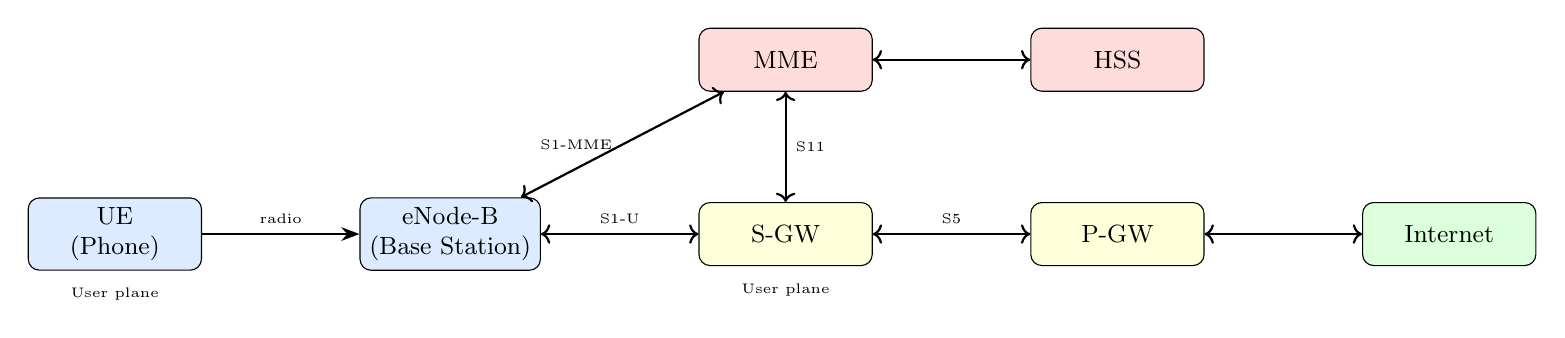
\begin{tikzpicture}[
    node distance=1.4cm and 2cm,
    box/.style={draw, rounded corners, minimum width=2.2cm, minimum height=0.8cm, align=center, font=\small},
    arr/.style={-Stealth, thick}
]
\node[box, fill=lightblue] (UE) {UE\\(Phone)};
\node[box, fill=lightblue, right=of UE] (eNB) {eNode-B\\(Base Station)};
\node[box, fill=lightyellow, right=of eNB] (SGW) {S-GW};
\node[box, fill=lightyellow, right=of SGW] (PGW) {P-GW};
\node[box, fill=lightred, above=of SGW] (MME) {MME};
\node[box, fill=lightred, above=of PGW] (HSS) {HSS};
\node[box, fill=lightgreen, right=of PGW] (Internet) {Internet};

\draw[arr] (UE) -- node[above,font=\tiny]{radio} (eNB);
\draw[arr, <->] (eNB) -- node[above,font=\tiny]{S1-U} (SGW);
\draw[arr, <->] (SGW) -- node[above,font=\tiny]{S5} (PGW);
\draw[arr, <->] (PGW) -- (Internet);
\draw[arr, <->] (MME) -- node[right,font=\tiny]{S11} (SGW);
\draw[arr, <->] (MME) -- (HSS);
\draw[arr, <->] (MME) -- node[left,font=\tiny]{S1-MME} (eNB);

\node[font=\tiny, below=0.1cm of UE] {User plane};
\node[font=\tiny, below=0.1cm of SGW] {User plane};
\end{tikzpicture}

\subsection{LTE Data Plane -- Tunneling}

\begin{keybox}[LTE Tunneling -- GTP-U Protocol]
In LTE, user data is \textbf{tunneled} from eNode-B all the way to P-GW using \textbf{GTP-U (GPRS Tunneling Protocol -- User plane)}:

\medskip
\textbf{Tunnel path:} UE $\leftrightarrow$ eNB $\xrightarrow{\text{GTP tunnel}}$ S-GW $\xrightarrow{\text{GTP tunnel}}$ P-GW $\leftrightarrow$ Internet

\begin{itemize}[noitemsep]
    \item Each user datagram is encapsulated in a GTP-U header (which adds a Tunnel Endpoint ID -- TEID).
    \item eNB $\rightarrow$ S-GW: one GTP tunnel per UE.
    \item S-GW $\rightarrow$ P-GW: another GTP tunnel per UE.
    \item The tunnels allow user traffic to flow transparently regardless of which eNB the UE is attached to.
\end{itemize}

\medskip
\textbf{Why tunneling?} Hides radio-network mobility from the IP core. When a UE moves between eNBs (handover), only the tunnel endpoints change -- the P-GW IP and the UE's allocated IP remain constant.
\end{keybox}

\subsection{LTE Link Layer}

\begin{keybox}[LTE Radio Access -- OFDM and Link-Layer Protocols]
\textbf{Physical layer:} LTE uses \textbf{OFDM (Orthogonal Frequency Division Multiplexing)}:
\begin{itemize}[noitemsep]
    \item Frequency band divided into many narrow orthogonal subcarriers.
    \item Combined FDM (across subcarriers) + TDM (time slots) = \textbf{OFDMA} in downlink.
    \item Each 1 ms subframe is divided into resource blocks (time $\times$ frequency) allocated to UEs by the base station scheduler.
    \item Each UE's resource block can use a different modulation/coding scheme (adaptive modulation per UE).
\end{itemize}

\medskip
\textbf{LTE link layer sub-layers} (between UE and eNB):
\begin{enumerate}[noitemsep]
    \item \textbf{PDCP (Packet Data Convergence Protocol):} IP header compression, ciphering (encryption).
    \item \textbf{RLC (Radio Link Control):} Fragmentation and reassembly of large packets. Reliable data transfer (ARQ -- Automatic Repeat reQuest).
    \item \textbf{MAC (Medium Access Control):} Scheduling, HARQ (Hybrid ARQ -- combines FEC + ARQ).
\end{enumerate}
\end{keybox}

\subsection{BS Association and Sleep Modes}

\begin{keybox}[BS Association in LTE]
How a UE connects to an eNB:
\begin{enumerate}[noitemsep]
    \item eNBs broadcast \textbf{synchronization signals} every 5 ms on a set of well-known frequencies.
    \item UE scans frequencies, detects synch signals, measures signal strength from multiple eNBs.
    \item UE selects the best eNB (strongest signal / highest SINR).
    \item UE sends \textbf{Random Access} message to eNB (contention-based RACH or contention-free).
    \item eNB responds with timing alignment and temporary ID.
    \item Authentication via MME and HSS: IMSI sent, HSS verifies subscriber, session established.
    \item P-GW assigns UE an IP address (via MME $\rightarrow$ S-GW $\rightarrow$ P-GW signaling).
\end{enumerate}
\end{keybox}

\begin{keybox}[LTE Sleep Modes -- DRX]
To save battery, LTE uses \textbf{DRX (Discontinuous Reception)} with two sleep modes:
\begin{itemize}[noitemsep]
    \item \textbf{Light sleep:} Wake up every 100s of milliseconds to check for downlink activity. Used when device is active but idle momentarily.
    \item \textbf{Deep sleep:} Sleep for 5--10 seconds. Used for longer idle periods (e.g., app in background). Device must re-establish connection more fully on wakeup.
\end{itemize}
\textbf{Tradeoff:} Deeper sleep $\rightarrow$ more battery savings, but longer latency to resume data transfer.
\end{keybox}

\subsection{4G vs.\ 5G}

\begin{keybox}[4G vs.\ 5G -- Key Differences]
\begin{center}
\begin{tabular}{lll}
\toprule
\textbf{Feature} & \textbf{4G LTE} & \textbf{5G NR} \\
\midrule
Peak downlink rate & $\sim$1 Gbps & Up to 20 Gbps \\
Latency & $\sim$30--50 ms & $<$1 ms (target) \\
Frequency bands & Sub-6 GHz & Sub-6 GHz + mmWave \\
Mobility & Full support & Full support \\
Architecture & Partial C/U-plane separation & Complete C/U-plane separation \\
Base station & eNode-B & gNode-B (gNB) \\
Core network & EPC & 5GC (5G Core) \\
\bottomrule
\end{tabular}
\end{center}

\medskip
\textbf{Key facts for exams:}
\begin{itemize}[noitemsep]
    \item \textbf{Both 4G and 5G support mobility / handover.}
    \item \textbf{5G has higher peak bitrate} than 4G.
    \item 5G is designed for \emph{complete} control/user-plane separation (4G has partial separation).
    \item 5G mmWave (millimeter wave, 24--100 GHz) offers very high rates but short range and limited penetration.
    \item 5G sub-6 GHz offers better range and coverage.
\end{itemize}
\end{keybox}

\begin{exambox}[Exam -- 4G/5G Statements - V23 Q1.4.5]
\textbf{V23 Q1.4.5 -- Which statements about 4G and 5G are true?}
\begin{itemize}[noitemsep]
    \item \textbf{a) 5G has higher peak bitrate than 4G.} \checkmark\ \textbf{TRUE} -- up to 20 Gbps vs.\ $\sim$1 Gbps.
    \item b) Only 5G supports mobility/handover; 4G does not. \texttimes\ FALSE -- both support mobility.
    \item \textbf{c) Both 4G and 5G support host mobility.} \checkmark\ \textbf{TRUE}
    \item d) 4G uses complete control/user-plane separation but 5G does not. \texttimes\ FALSE -- 5G is the one designed for \emph{complete} separation.
    \item e) 5G uses CSMA/CA for medium access. \texttimes\ FALSE -- that is 802.11 WiFi. LTE/5G use OFDMA and scheduled access.
\end{itemize}

\medskip
\textbf{Remember:} 5G = higher rate + lower latency + complete C/U-plane separation + both support mobility.
\end{exambox}

%=============================================================================
\section{Putting It All Together -- Wireless Summary}
%=============================================================================

\begin{keybox}[Chapter 7 -- Big Picture Summary]
\textbf{Why is wireless hard?} Three challenges: path loss, interference, multipath. These cause higher and variable BER compared to wired links.

\medskip
\textbf{SNR/BER tradeoff:} Higher SNR $\Rightarrow$ lower BER. Higher-order modulation $\Rightarrow$ higher BER at same SNR but higher throughput. Rate adaptation dynamically picks the best modulation for current channel conditions.

\medskip
\textbf{802.11 MAC:} CSMA/CA (not CD). DIFS before transmission. Random backoff (timer freezes during busy channel). Full-frame transmission. ACK after SIFS. RTS/CTS for hidden terminal mitigation.

\medskip
\textbf{802.11 frames:} 4 MAC addresses (Addr1=receiver, Addr2=transmitter, Addr3=router, Addr4=ad hoc). Frame control field encodes type, subtype, power management, WEP, To/From DS bits.

\medskip
\textbf{4G LTE:} UE $\leftrightarrow$ eNB (radio) $\leftrightarrow$ S-GW $\leftrightarrow$ P-GW $\leftrightarrow$ Internet (data plane). MME handles control (auth, mobility). HSS stores subscriber data. IMSI identifies subscriber on SIM. GTP-U tunneling end-to-end. OFDM/OFDMA radio access.

\medskip
\textbf{5G vs.\ 4G:} Higher peak rate, lower latency, complete C/U-plane separation. Both support mobility.
\end{keybox}

\begin{warnbox}[Common Exam Traps -- Chapter 7]
\begin{itemize}[noitemsep]
    \item \textbf{CSMA/CD vs.\ CSMA/CA:} 802.11 uses CA (avoidance), \emph{not} CD (detection). Wired Ethernet uses CD.
    \item \textbf{Who sends CTS?} The \emph{AP} sends CTS in response to sender's RTS -- not the sender.
    \item \textbf{Backoff timer behavior:} Timer counts down only when channel is \emph{idle}. It \emph{freezes} (not resets) when channel goes busy.
    \item \textbf{Higher SNR = better:} Do not confuse direction. Lower SNR $\Rightarrow$ higher BER $\Rightarrow$ worse performance.
    \item \textbf{Higher modulation = more fragile:} QAM-256 is faster but needs good channel. BPSK is slow but robust.
    \item \textbf{Both 4G and 5G have mobility:} A common distractor says only 5G supports mobility -- false.
    \item \textbf{5G does not use CSMA/CA:} CSMA/CA is 802.11 WiFi. LTE and 5G use OFDMA with base-station scheduling.
    \item \textbf{RTS/CTS reduces but doesn't eliminate hidden terminal:} Two nodes can still collide on their RTS frames.
\end{itemize}
\end{warnbox}

\begin{formulabox}[Quick Reference -- Key Numbers]
\begin{itemize}[noitemsep]
    \item 802.11b: 2.4 GHz, 11 Mbps
    \item 802.11g: 2.4 GHz, 54 Mbps
    \item 802.11n (WiFi 4): 2.4/5 GHz, 600 Mbps (MIMO)
    \item 802.11ac (WiFi 5): 5 GHz, 3.47 Gbps (MU-MIMO)
    \item 802.11ax (WiFi 6): 2.4/5/6 GHz, 14 Gbps (OFDMA)
    \item 802.11 beacon interval: $\sim$100 ms
    \item LTE synch signal: every 5 ms
    \item LTE light sleep: 100s of ms; deep sleep: 5--10 s
    \item LTE IMSI: 64 bits on SIM card
    \item 4G peak: $\sim$1 Gbps; 5G peak: $\sim$20 Gbps
\end{itemize}
\end{formulabox}


% ============================================================
%  CHAPTER 8
% ============================================================
\chapterdivider{8}{Chapter 8: Security}
\section{What Is Network Security?}
% ═══════════════════════════════════════════════════════════════════════════════

\begin{tcolorbox}[keybox, title=Four Desirable Properties of Secure Communication]
\begin{enumerate}[noitemsep]
  \item \textbf{Confidentiality} -- only sender and intended receiver should understand message contents (message encrypted)
  \item \textbf{Authentication} -- sender and receiver can confirm each other's identity
  \item \textbf{Message integrity} -- message not altered in transit (without detection)
  \item \textbf{Access and availability} -- services must be accessible and available to authorised users (operational security)
\end{enumerate}
\end{tcolorbox}

\subsection{The Language of Cryptography}

The standard model uses three actors:
\begin{itemize}[noitemsep]
  \item \textbf{Alice} -- legitimate sender
  \item \textbf{Bob} -- legitimate receiver
  \item \textbf{Trudy} -- the intruder
\end{itemize}

\begin{tcolorbox}[warnbox, title=What Trudy Can Do]
\begin{itemize}[noitemsep]
  \item \textbf{Eavesdrop} -- intercept/record messages (sniff control and data messages)
  \item \textbf{Insert} -- insert messages into the connection
  \item \textbf{Impersonate} -- fake source address in packet (IP spoofing)
  \item \textbf{Hijack} -- take over an ongoing connection by removing sender or receiver
  \item \textbf{Denial of Service} -- prevent service from being used (e.g., SYN flooding)
  \item \textbf{Modify or delete} -- alter or remove message content
\end{itemize}
\end{tcolorbox}

\begin{tcolorbox}[keybox, title=Cryptography Notation]
\begin{itemize}[noitemsep]
  \item Plaintext message: $m$
  \item Encryption algorithm: $K_A(\cdot)$ using key $K_A$
  \item Ciphertext: $c = K_A(m)$
  \item Decryption: $m = K_B(K_A(m))$
  \item \textbf{Symmetric key:} $K_A = K_B$ (same shared secret key)
  \item \textbf{Public key pair:} $K_B^+$ (Bob's public key), $K_B^-$ (Bob's private key)
  \item Key property: $K_B^-(K_B^+(m)) = m$ \quad and \quad $K_B^+(K_B^-(m)) = m$
\end{itemize}
\end{tcolorbox}

% ═══════════════════════════════════════════════════════════════════════════════
\section{Symmetric Key Cryptography}
% ═══════════════════════════════════════════════════════════════════════════════

Both parties share the same secret key. Key problem: how do two parties agree on a key in the first place?

\subsection{Substitution Ciphers}

\begin{tcolorbox}[keybox, title=Caesar Cipher -- Simple Substitution]
\begin{itemize}[noitemsep]
  \item Replace each letter by a letter $k$ positions later in alphabet (wrapping around)
  \item Encode: shift letter by $+k$; Decode: shift by $-k$
  \item Example ($k=3$): ``abc'' $\rightarrow$ ``def''; ``xyz'' $\rightarrow$ ``abc''
  \item Only 25 possible keys -- trivially brute-forced
  \item \textbf{Monoalphabetic cipher:} substitute letter for letter (26! possible mappings). Breakable by frequency analysis
\end{itemize}
\end{tcolorbox}

\begin{tcolorbox}[formulabox, title=Caesar Cipher Example -- k=7]
Encode ``Protect'' with $k=7$:\\
P$\to$W, r$\to$y, o$\to$v, t$\to$a, e$\to$l, c$\to$j, t$\to$a $\Rightarrow$ \texttt{Wyvaljapvu}\\[4pt]
Decode ``Jhlzhy'' with $k=7$ (subtract 7):\\
J$\to$C, h$\to$a, l$\to$e, z$\to$s, h$\to$a, y$\to$r $\Rightarrow$ \texttt{Caesar}
\end{tcolorbox}

\subsection{DES -- Data Encryption Standard}

\begin{tcolorbox}[keybox, title=DES]
\begin{itemize}[noitemsep]
  \item 56-bit key, 64-bit block encryption
  \item 16 rounds of permutation/substitution using subkeys derived from main key
  \item \textbf{CBC -- Cipher Block Chaining:} each plaintext block XOR-ed with previous ciphertext block before encryption; prevents identical plaintext blocks producing identical ciphertext
  \item \textbf{Security:} Brute-forceable in under 1 day with today's hardware (too weak)
  \item \textbf{3DES:} encrypt with $K_1$, decrypt with $K_2$, encrypt with $K_3$ -- effectively 168-bit key
\end{itemize}
\end{tcolorbox}

\subsection{AES -- Advanced Encryption Standard}

\begin{tcolorbox}[keybox, title=AES]
\begin{itemize}[noitemsep]
  \item 128-bit blocks; key length: 128, 192, or 256 bits
  \item At 1 billion DES keys/second: $2^{128}$ AES combinations $\approx$ \textbf{149 trillion years} to brute-force
  \item Replaced DES as US standard (NIST 2001)
  \item Used in TLS, 802.11 WPA2/WPA3, 4G LTE (AES on the radio link)
\end{itemize}
\end{tcolorbox}

\begin{tcolorbox}[warnbox, title=Symmetric Key Problem]
$n$ people wanting to communicate privately with each other all require \textbf{unique pairwise keys}:
\[ \text{Number of keys} = \frac{n(n-1)}{2} \]
Example: 10 people need $\frac{10 \times 9}{2} = 45$ keys. Scales poorly for large groups.
\end{tcolorbox}

% ═══════════════════════════════════════════════════════════════════════════════
\section{Public Key Cryptography}
% ═══════════════════════════════════════════════════════════════════════════════

\begin{tcolorbox}[keybox, title=Public Key Cryptography -- Key Idea]
\begin{itemize}[noitemsep]
  \item Everyone has a \textbf{public key} $K^+$ (known to all) and a \textbf{private key} $K^-$ (secret)
  \item Anyone can encrypt with public key; only owner can decrypt with private key
  \item \textbf{Solves} the symmetric key distribution problem -- no shared secret needed upfront
  \item Mathematical requirement: $K^-(K^+(m)) = m$ and $K^+(K^-(m)) = m$
  \item Computationally infeasible to derive $K^-$ from $K^+$
\end{itemize}
\end{tcolorbox}

\begin{imagebox}[Symmetric vs.\ Public Key Cryptography]
\textbf{Textbook:} Kurose \& Ross 8e, Figure 8.2 (Symmetric key cryptography) and Figure 8.6 (Public key cryptography)\\
\textbf{Google:} ``symmetric vs asymmetric key cryptography diagram comparison''\\
\textit{Why: Shows how symmetric uses one shared key while public key uses a key pair for encryption/decryption.}
\end{imagebox}

\begin{tcolorbox}[warnbox, title=Key Difference -- Symmetric vs.\ Public Key]
\begin{tabular}{lll}
\toprule
\textbf{Property} & \textbf{Symmetric} & \textbf{Public Key} \\
\midrule
Keys needed & $n(n-1)/2$ & $2n$ -- one pair per person \\
Key distribution & Requires secure channel & Public key openly shared \\
Speed & Very fast & Computationally expensive \\
Use in practice & Bulk data encryption & Key exchange, signatures \\
\bottomrule
\end{tabular}
\end{tcolorbox}

\subsection{RSA -- Rivest, Shamir, Adleman}

\begin{tcolorbox}[formulabox, title=RSA -- How It Works]
\textbf{Key generation:}
\begin{enumerate}[noitemsep]
  \item Choose two large primes $p$ and $q$ (1024 bits each)
  \item Compute $n = p \cdot q$ and $z = (p-1)(q-1)$
  \item Choose $e$ such that $e < n$ and $\gcd(e,z) = 1$
  \item Find $d$ such that $ed \equiv 1 \pmod{z}$
  \item Public key: $(n, e)$; Private key: $(n, d)$
\end{enumerate}
\textbf{Encrypt:} $c = m^e \bmod n$ \quad \textbf{Decrypt:} $m = c^d \bmod n$\\[4pt]
\textbf{Security basis:} factoring a large number $n$ into $p \cdot q$ is computationally infeasible.\\[4pt]
\textbf{Important property:} $K_B^-(K_B^+(m)) = m$ \textit{and} $K_B^+(K_B^-(m)) = m$ -- can apply in either order.
\end{tcolorbox}

\begin{imagebox}[RSA Public Key Encryption]
\textbf{Textbook:} Kurose \& Ross 8e, Figure 8.6 (RSA public key encryption)\\
\textbf{Google:} ``RSA encryption algorithm example key generation diagram''\\
\textit{Why: Illustrates RSA key generation, encryption ($c = m^e \bmod n$), and decryption ($m = c^d \bmod n$) step by step.}
\end{imagebox}

% ═══════════════════════════════════════════════════════════════════════════════
\section{Authentication and Message Integrity}
% ═══════════════════════════════════════════════════════════════════════════════

\subsection{Message Integrity and Hash Functions}

\begin{tcolorbox}[keybox, title=Cryptographic Hash Functions]
A hash function $H(m)$ produces a fixed-length \textbf{message digest}. Properties required:
\begin{itemize}[noitemsep]
  \item Many-to-one: maps arbitrary-length $m$ to fixed-length digest
  \item \textbf{Computationally infeasible} to find two messages with the same hash
  \item \textbf{Computationally infeasible} to find $m$ given $H(m)$
  \item A small change in $m$ produces a completely different hash
\end{itemize}
\textbf{Common hash algorithms:}
\begin{itemize}[noitemsep]
  \item \textbf{MD5:} 128-bit digest (RFC 1321) -- now considered weak
  \item \textbf{SHA-1:} 160-bit digest -- widely used
  \item \textbf{SHA-256:} 256-bit digest -- current standard
\end{itemize}
\textbf{Note:} Internet checksum is NOT a cryptographic hash -- too easy to find collisions. Hash is strictly better than checksum for integrity.
\end{tcolorbox}

\subsection{Message Authentication Code -- HMAC}

\begin{tcolorbox}[keybox, title=HMAC -- Hash-based Message Authentication Code]
\textbf{Problem:} A plain hash $H(m)$ doesn't prove who created the message -- Trudy can modify $m$ and recompute $H(m)$.\\[4pt]
\textbf{Solution -- HMAC:} combine message with a shared secret $s$:
\[ \text{MAC} = H(m + s) \]
\begin{itemize}[noitemsep]
  \item Only parties who know secret $s$ can compute or verify the MAC
  \item Receiver checks: recompute $H(m+s)$ and compare with received MAC
  \item Used in TLS, 802.11 WPA2, 4G LTE
\end{itemize}
\end{tcolorbox}

\subsection{Digital Signatures}

\begin{tcolorbox}[keybox, title=Digital Signatures]
\textbf{Goal:} verifiable, non-repudiable -- Bob can prove to others that Alice sent this exact message.\\[4pt]
\textbf{How Bob signs message $m$:}
\begin{enumerate}[noitemsep]
  \item Compute hash: $H(m)$
  \item Encrypt hash with his private key: $K_B^-(H(m))$ -- this is the \textbf{digital signature}
  \item Send $m$ and $K_B^-(H(m))$ together
\end{enumerate}
\textbf{Verification by receiver:}
\begin{enumerate}[noitemsep]
  \item Decrypt signature with Bob's public key: $K_B^+(K_B^-(H(m))) = H(m)$
  \item Independently compute $H(m)$ from the received message
  \item If they match $\Rightarrow$ message is authentic and unaltered
\end{enumerate}
\textbf{Properties:}
\begin{itemize}[noitemsep]
  \item \textbf{Non-repudiation:} only Bob could have produced $K_B^-(H(m))$
  \item Protects against both alteration and false authorship claims
\end{itemize}
\end{tcolorbox}

\begin{imagebox}[Digital Signatures and Message Digests]
\textbf{Textbook:} Kurose \& Ross 8e, Figure 8.9 (Digital signatures) and Figure 8.12 (Message digests)\\
\textbf{Google:} ``digital signature hash message authentication diagram''\\
\textit{Why: Shows how a sender signs a hash of the message with their private key, and the receiver verifies it with the public key.}
\end{imagebox}

\subsection{Certification Authorities -- CAs}

\begin{tcolorbox}[keybox, title=Public Key Infrastructure and CAs]
\textbf{Problem:} How do you know a public key really belongs to who claims it?\\[4pt]
\textbf{Solution:} Certification Authority (CA) binds a public key to a specific entity.
\begin{enumerate}[noitemsep]
  \item Entity provides their public key to CA along with proof of identity
  \item CA creates a \textbf{certificate} containing the entity's public key, signed with CA's private key
  \item Anyone who trusts the CA can verify the certificate using the CA's public key
\end{enumerate}
\textbf{Browser trust:} Web browsers come pre-installed with certificates from well-known CAs (e.g., VeriSign, Comodo). This forms the \textbf{chain of trust}.\\[4pt]
\textbf{Certificate contents:} entity name, public key, valid date range, CA name, CA digital signature
\end{tcolorbox}

% ═══════════════════════════════════════════════════════════════════════════════
\section{Secure E-mail}
% ═══════════════════════════════════════════════════════════════════════════════

\begin{tcolorbox}[keybox, title=Secure E-mail -- All Three Goals]
Secure e-mail combines public key, symmetric key, and hashing to provide confidentiality, authentication, and integrity.\\[6pt]
\textbf{Alice wants to send confidential, authenticated, integrity-protected message to Bob:}
\begin{enumerate}[noitemsep]
  \item Generate random \textbf{symmetric session key} $K_S$
  \item Encrypt message: $K_S(m)$ -- fast symmetric encryption for the bulk data
  \item Encrypt session key with Bob's public key: $K_B^+(K_S)$ -- only Bob can recover $K_S$
  \item Compute hash $H(m)$ and sign with Alice's private key: $K_A^-(H(m))$ -- authentication + integrity
  \item Send: $K_S(m)$, $K_B^+(K_S)$, $K_A^-(H(m))$
\end{enumerate}
\textbf{Three keys used:} $K_S$ (session), $K_B^+$ (Bob's public), $K_A^-$ (Alice's private)\\[4pt]
\textbf{Bob's decryption:}
\begin{enumerate}[noitemsep]
  \item Use $K_B^-$ to decrypt $K_B^+(K_S)$ $\Rightarrow$ recover $K_S$
  \item Use $K_S$ to decrypt $K_S(m)$ $\Rightarrow$ recover $m$
  \item Use Alice's $K_A^+$ to verify signature $\Rightarrow$ confirm integrity and authenticity
\end{enumerate}
\end{tcolorbox}

% ═══════════════════════════════════════════════════════════════════════════════
\section{TLS -- Transport Layer Security}
% ═══════════════════════════════════════════════════════════════════════════════

\begin{tcolorbox}[keybox, title=TLS Overview]
\begin{itemize}[noitemsep]
  \item \textbf{HTTPS} = HTTP over TLS; port \textbf{443}
  \item TLS sits between the application layer and TCP -- a ``sublayer'' of the transport layer
  \item Provides: \textbf{confidentiality} via symmetric encryption, \textbf{integrity} via MAC/hashing, \textbf{authentication} via certificates (public key)
  \item Successor to SSL (Secure Sockets Layer)
\end{itemize}
\end{tcolorbox}

\subsection{TLS Handshake}

\begin{tcolorbox}[keybox, title=TLS Handshake Steps]
\begin{enumerate}[noitemsep]
  \item \textbf{TCP 3-way handshake} -- establish TCP connection
  \item \textbf{TLS Hello} -- client sends list of supported cipher suites and a \textbf{nonce} (random number)
  \item \textbf{Server responds} with: chosen cipher suite, server \textbf{certificate} (containing public key), server nonce
  \item \textbf{Client verifies} certificate against trusted CAs
  \item \textbf{Client sends} Pre-Master Secret (PMS) encrypted with server's public key: $K_S^+(PMS)$
  \item Both sides independently derive the same \textbf{4 session keys} from PMS and nonces:
    \begin{itemize}[noitemsep]
      \item $E_A$ -- client-to-server encryption key
      \item $M_A$ -- client-to-server MAC key
      \item $E_B$ -- server-to-client encryption key
      \item $M_B$ -- server-to-client MAC key
    \end{itemize}
  \item \textbf{Encrypted Handshake Message} -- each side sends MAC of entire handshake to confirm agreement
\end{enumerate}
\end{tcolorbox}

\subsection{TLS Records and TLS 1.3}

\begin{tcolorbox}[keybox, title=TLS Records]
Each TLS record contains:
\begin{itemize}[noitemsep]
  \item Type, version, length fields
  \item Encrypted data
  \item \textbf{MAC} (Message Authentication Code) -- computed over data + sequence number, using key $M_A$ or $M_B$
\end{itemize}
Sequence numbers prevent \textbf{replay attacks} -- an attacker cannot re-send an old TLS record.
\end{tcolorbox}

\begin{imagebox}[The SSL/TLS Handshake]
\textbf{Textbook:} Kurose \& Ross 8e, Figure 8.18 (The SSL/TLS handshake)\\
\textbf{Google:} ``TLS SSL handshake diagram client hello server hello''\\
\textit{Why: Shows the sequence of messages (ClientHello, ServerHello, certificate, key exchange) that establish a TLS session.}
\end{imagebox}

\begin{tcolorbox}[warnbox, title=TLS 1.3 Changes]
TLS 1.3 (current version) tightens the cipher suite to only 5 choices:
\begin{itemize}[noitemsep]
  \item Requires \textbf{Diffie-Hellman} for key exchange (provides forward secrecy)
  \item Requires \textbf{HMAC-SHA} for integrity
  \item Removes weak options (RSA key exchange, CBC-mode ciphers, MD5)
  \item Faster handshake (1-RTT instead of 2-RTT)
\end{itemize}
\end{tcolorbox}

% ═══════════════════════════════════════════════════════════════════════════════
\section{Network Layer Security -- IPsec and VPNs}
% ═══════════════════════════════════════════════════════════════════════════════

\subsection{VPN -- Virtual Private Network}

\begin{tcolorbox}[keybox, title=VPN]
\begin{itemize}[noitemsep]
  \item Institution's traffic sent over the public Internet but \textbf{encrypted} end-to-end
  \item Creates an encrypted ``tunnel'' so external traffic appears as normal IP packets
  \item Implemented using \textbf{IPsec} at the network layer
  \item Remote employees can securely access institutional resources over the public Internet
\end{itemize}
\end{tcolorbox}

\subsection{IPsec}

\begin{tcolorbox}[keybox, title=IPsec Services]
IPsec provides network-layer security with four services:
\begin{enumerate}[noitemsep]
  \item \textbf{Data integrity} -- receiver can detect any modification of datagram in transit
  \item \textbf{Origin authentication} -- receiver can verify source of IPsec datagram
  \item \textbf{Replay attack prevention} -- sequence numbers prevent old packets being replayed
  \item \textbf{Confidentiality} -- payload encrypted (in ESP mode)
\end{enumerate}
\end{tcolorbox}

\begin{tcolorbox}[keybox, title=IPsec Modes and Protocols]
\textbf{Transport mode:} only the IP payload is encrypted/authenticated; original IP header untouched\\
\textbf{Tunnel mode:} entire IP datagram is encrypted + authenticated and encapsulated in a new IP datagram (used in VPNs)\\[6pt]
\textbf{Two IPsec protocols:}
\begin{itemize}[noitemsep]
  \item \textbf{AH -- Authentication Header:} provides integrity and authentication but \textit{no} confidentiality
  \item \textbf{ESP -- Encapsulating Security Payload:} provides integrity, authentication, \textit{and} confidentiality -- far more commonly used
\end{itemize}
\end{tcolorbox}

\begin{imagebox}[IPsec Datagram Structure]
\textbf{Textbook:} Kurose \& Ross 8e, Figure 8.22 (IPsec datagram)\\
\textbf{Google:} ``IPsec tunnel transport mode ESP AH diagram''\\
\textit{Why: Shows the structure of an IPsec datagram in tunnel vs.\ transport mode, with ESP/AH header placement.}
\end{imagebox}

% ═══════════════════════════════════════════════════════════════════════════════
\section{Security in Wireless and Mobile Networks}
% ═══════════════════════════════════════════════════════════════════════════════

\subsection{802.11 WiFi Security -- WPA2/WPA3}

\begin{tcolorbox}[keybox, title=802.11 Security -- 4-Step Process]
\begin{enumerate}[noitemsep]
  \item \textbf{Discovery:} AP advertises its presence and security capabilities (encryption/authentication suites)
  \item \textbf{Mutual authentication and key derivation:} using WPA2/WPA3 and an Authentication Server (AS); shared master key established; uses \textbf{nonces} (random numbers) to generate session key
  \item \textbf{Shared session key distribution:} pairwise transient key derived from master key; AP installs key for communicating with this device
  \item \textbf{Encrypted communication:} data encrypted using the derived session key (AES-based in WPA2)
\end{enumerate}
\end{tcolorbox}

\begin{tcolorbox}[formulabox, title=WPA2 Key Derivation Using Nonces]
\begin{enumerate}[noitemsep]
  \item AS sends nonce $N_{AS}$ to mobile
  \item Mobile sends nonce $N_M$ to AS
  \item Both sides derive the same \textbf{Pairwise Master Key} from shared master key + nonces using HMAC
  \item Session key derived from PMK -- protects mobile-to-AP communication
\end{enumerate}
Nonces prevent replay attacks: even if Trudy captures the exchange, she cannot reuse it.
\end{tcolorbox}

\subsection{4G LTE Authentication and Encryption}

\begin{tcolorbox}[keybox, title=4G LTE Authentication -- 5 Steps]
\textbf{Actors:} Mobile device (SIM with shared key $K_{HSS-M}$), Base Station (BS), Mobility Management Entity (MME), Home Subscriber Service (HSS)\\[6pt]
\begin{enumerate}[noitemsep]
  \item[\textbf{a}] \textbf{Mobile attaches} -- sends IMSI (identity) to BS $\to$ MME; MME sends \texttt{AUTH\_REQ(IMSI, VN info)} to HSS
  \item[\textbf{b}] \textbf{HSS responds} -- HSS derives authentication token + expected response $xres_{HSS}$ from $K_{HSS-M}$; sends \texttt{AUTH\_RESP(auth\_token, xres\_{HSS}, keys)} back to MME
  \item[\textbf{c}] \textbf{Mobile authenticates network} -- mobile receives auth token, verifies it using its $K_{HSS-M}$ (proves HSS is legitimate); mobile computes $res_M$ using same crypto as HSS
  \item[\textbf{d}] \textbf{Network authenticates mobile} -- mobile sends $res_M$ to MME; MME compares $res_M$ with $xres_{HSS}$; if match $\Rightarrow$ mobile authenticated; MME generates keys for BS
  \item[\textbf{e}] \textbf{Key derivation} -- mobile and BS determine session keys for encrypting data and control frames; \textbf{AES} can be used on the 4G radio link
\end{enumerate}
\textbf{Note:} MME + HSS together play the role of the Authentication Server (analogous to WiFi AS).
\end{tcolorbox}

\begin{tcolorbox}[warnbox, title=4G LTE Key Insight]
The SIM card stores the shared secret $K_{HSS-M}$ which is also stored at the HSS. Authentication is \textbf{mutual}: the mobile verifies the network (prevents fake BS attacks), and the network verifies the mobile. The session key $K_{BS-M}$ used for radio link encryption is derived fresh each session.
\end{tcolorbox}

% ═══════════════════════════════════════════════════════════════════════════════
\section{Operational Security -- Firewalls}
% ═══════════════════════════════════════════════════════════════════════════════

\begin{tcolorbox}[keybox, title=Firewall Definition]
A \textbf{firewall} isolates an organisation's internal network from the larger Internet, allowing some packets to pass and blocking others. It sits between the trusted internal network and the untrusted public Internet.
\end{tcolorbox}

\subsection{Three Goals of Firewalls}

\begin{tcolorbox}[keybox, title=Why Firewalls -- Three Goals]
\begin{enumerate}[noitemsep]
  \item \textbf{Prevent denial-of-service attacks} -- e.g., SYN flooding: attacker establishes many bogus TCP connections, consuming resources so no capacity remains for legitimate connections
  \item \textbf{Prevent illegal modification/access of internal data} -- e.g., attacker replaces a web page with malicious content
  \item \textbf{Allow only authorised access to inside network} -- authenticate users/hosts; block all other access
\end{enumerate}
\textbf{Three types of firewalls:} stateless packet filters, stateful packet filters, application gateways
\end{tcolorbox}

\subsection{Stateless Packet Filtering}

\begin{tcolorbox}[keybox, title=Stateless Packet Filtering]
\begin{itemize}[noitemsep]
  \item Internal network connected to Internet via a \textbf{router firewall}
  \item Filters \textbf{packet-by-packet}; decision to forward or drop based on:
    \begin{itemize}[noitemsep]
      \item Source/destination IP address
      \item TCP/UDP source and destination port numbers
      \item ICMP message type
      \item TCP SYN and ACK bits
    \end{itemize}
  \item Uses an \textbf{ACL -- Access Control List}: table of (action, condition) pairs applied top to bottom
\end{itemize}
\end{tcolorbox}

\begin{tcolorbox}[formulabox, title=ACL Examples -- Policy to Firewall Setting]
\begin{tabular}{p{5.5cm}p{6.5cm}}
\toprule
\textbf{Policy} & \textbf{Firewall Setting} \\
\midrule
No outside Web access & Drop all outgoing packets to any IP, port 80 \\
No incoming TCP connections except to institution's public Web server & Drop all incoming TCP SYN to any IP except 130.207.244.203, port 80 \\
Prevent Web-radios eating bandwidth & Drop all incoming UDP -- except DNS and router broadcasts \\
Prevent smurf DoS attacks & Drop all ICMP to broadcast addresses \\
Prevent traceroute scanning & Drop all outgoing ICMP TTL-expired traffic \\
Block all incoming UDP + telnet & Block protocol=17, port=23; also block ACK=0 inbound TCP \\
\bottomrule
\end{tabular}
\end{tcolorbox}

\begin{tcolorbox}[warnbox, title=Stateless Packet Filter Weakness]
A stateless filter is a ``heavy-handed tool'' -- it can admit packets that \textbf{make no sense} given the conversation state. For example, allowing inbound TCP ACK packets even when no TCP connection to that destination was ever initiated. An attacker can craft such packets to exploit this.
\end{tcolorbox}

\subsection{Stateful Packet Filtering}

\begin{tcolorbox}[keybox, title=Stateful Packet Filtering]
\begin{itemize}[noitemsep]
  \item Tracks the \textbf{state of every TCP connection} -- SYN, SYN-ACK, ACK, FIN
  \item Determines whether incoming/outgoing packets ``\textbf{make sense}'' given connection state
  \item ACL augmented with a ``check connection state table'' column
  \item Timeouts inactive connections -- stops admitting packets after connection ends
\end{itemize}
\textbf{Example:} A packet with ACK=1, destination port=80 is only admitted if there is an established TCP connection to port 80 in the state table. Without state tracking, this packet would pass even if no connection exists.
\end{tcolorbox}

\subsection{Application Gateways}

\begin{tcolorbox}[keybox, title=Application Gateways]
\begin{itemize}[noitemsep]
  \item Filter packets on \textbf{application-layer data} as well as IP/TCP/UDP fields
  \item Example: allow only selected internal users to telnet outside:
    \begin{enumerate}[noitemsep]
      \item All telnet users must connect to the gateway
      \item Gateway authenticates user; if authorised, sets up second telnet connection to destination
      \item Gateway relays data between the two connections
      \item Router filter blocks all telnet connections not originating from gateway
    \end{enumerate}
  \item Each application requires its own gateway (HTTP gateway, FTP gateway, etc.)
\end{itemize}
\end{tcolorbox}

\begin{imagebox}[Firewall Placement and Architecture]
\textbf{Textbook:} Kurose \& Ross 8e, Figure 8.28 (Firewall placement)\\
\textbf{Google:} ``network firewall DMZ architecture stateful packet filter diagram''\\
\textit{Why: Shows how a firewall is positioned between the internal network and the Internet, including DMZ architecture.}
\end{imagebox}

\subsection{Limitations of Firewalls and Gateways}

\begin{tcolorbox}[warnbox, title=Firewall Limitations]
\begin{itemize}[noitemsep]
  \item \textbf{IP spoofing:} router cannot verify data ``really'' comes from claimed source
  \item \textbf{Multiple app gateways needed:} each application requiring special treatment needs its own gateway
  \item \textbf{Client software must know gateway address} (e.g., proxy settings in browser)
  \item \textbf{UDP all-or-nothing:} filters often use all-or-nothing policy for UDP traffic
  \item \textbf{Tradeoff:} degree of communication with outside world vs.\ level of security
  \item \textbf{Not foolproof:} many highly protected sites still suffer attacks
\end{itemize}
\end{tcolorbox}

% ═══════════════════════════════════════════════════════════════════════════════
\section{Summary -- Where Security Is Applied}
% ═══════════════════════════════════════════════════════════════════════════════

\begin{tcolorbox}[keybox, title=Security Techniques Applied Across Layers]
\begin{tabular}{lll}
\toprule
\textbf{Scenario} & \textbf{Layer} & \textbf{Mechanisms Used} \\
\midrule
Secure e-mail & Application & Public key + symmetric + hash \\
HTTPS / TLS & Transport & Symmetric key + hash + certificates \\
VPN & Network & IPsec -- AH or ESP \\
IPsec & Network & AH or ESP (transport or tunnel mode) \\
802.11 WiFi & Link & WPA2/WPA3, HMAC, AES \\
4G LTE & Link/Physical & HMAC, AES over radio link \\
Firewalls & Network & Packet filtering, ACLs, state tables \\
\bottomrule
\end{tabular}
\end{tcolorbox}

% ═══════════════════════════════════════════════════════════════════════════════
\section{Exam Questions}
% ═══════════════════════════════════════════════════════════════════════════════

\begin{tcolorbox}[exambox, title=V23 Q1.5.1 -- Properties of Secure Communication]
\textbf{Which of the following are desirable properties of secure communication?}
\begin{itemize}[noitemsep]
  \item[a)] Network reliability
  \item[b)] \textbf{Confidentiality} \checkmark
  \item[c)] Message integrity \checkmark
  \item[d)] Authentication \checkmark
  \item[e)] Operational security \checkmark
  \item[f)] High bandwidth to transmit quickly
\end{itemize}
\textbf{Answer: b, c, d, e.} The four properties are confidentiality, authentication, message integrity, and operational security. Network reliability and bandwidth are not security properties.
\end{tcolorbox}

\begin{tcolorbox}[exambox, title=V23/V24 Q1.5.2 -- Number of Symmetric Keys]
\textbf{N people want to communicate privately using symmetric key encryption. How many keys are needed?}
\begin{itemize}[noitemsep]
  \item[a)] $N \times N$
  \item[b)] $2N - 1$
  \item[c)] $N(N-1)$
  \item[\textbf{d)}] $\mathbf{N(N-1)/2}$ \checkmark
  \item[e)] None of the above
\end{itemize}
\textbf{Answer: d.} Each pair of communicating parties needs a unique shared key. The number of unique pairs from $N$ people is $\binom{N}{2} = \frac{N(N-1)}{2}$.\\
\textbf{Example:} 10 people: $\frac{10 \times 9}{2} = 45$ keys.
\end{tcolorbox}

\begin{tcolorbox}[exambox, title=V23/V24 Q1.5.3 -- Message Integrity]
\textbf{For message integrity, which statements are correct?}
\begin{itemize}[noitemsep]
  \item[a)] Message integrity means confirming the identity of the sender
  \item[\textbf{b)}] \textbf{Message integrity means the receiver can detect whether the message was altered in transit} \checkmark
  \item[\textbf{c)}] \textbf{Both checksumming and hashing techniques may be used} \checkmark
  \item[\textbf{d)}] \textbf{Generally, a hash provides a better integrity check than a checksum} \checkmark
  \item[e)] To ensure message integrity, TCP must be used
\end{itemize}
\textbf{Answer: b, c, d.} Option a describes authentication, not integrity. Option e is false -- integrity can be ensured at any layer and does not require TCP.
\end{tcolorbox}

\begin{tcolorbox}[exambox, title=V24 Q1.5.4 -- HTTP Streaming vs.\ UDP Streaming]
\textbf{HTTP streaming over TCP is more popular than UDP streaming. Major reasons include:}
\begin{itemize}[noitemsep]
  \item[a)] UDP is connectionless
  \item[\textbf{b)}] \textbf{UDP lacks retransmission, ordering, and error-checking -- results in higher error rate} \checkmark
  \item[c)] UDP streaming has lower latency due to no handshakes
  \item[\textbf{d)}] \textbf{Many firewalls block UDP traffic but allow HTTP traffic} \checkmark
  \item[e)] None of the above
\end{itemize}
\textbf{Answer: b, d.} HTTP/TCP streaming benefits from reliability and passes through firewalls easily. Although UDP has lower latency, this is not a reason for HTTP being more popular; it is a reason in UDP's favour.
\end{tcolorbox}

\begin{tcolorbox}[exambox, title=V24 Q1.5.5 -- What Trudy Can Do -- Alice-Bob Model]
\textbf{Trudy is an intruder in the Alice-Bob model. Which actions can she take?}
\begin{itemize}[noitemsep]
  \item[\textbf{a)}] \textbf{Sniffing and recording control messages on the channel} \checkmark
  \item[\textbf{b)}] \textbf{Recording data messages on the channel} \checkmark
  \item[\textbf{c)}] \textbf{Modifying or insertion of messages} \checkmark
  \item[\textbf{d)}] \textbf{Deletion of message or message content} \checkmark
  \item[e)] None of the above
\end{itemize}
\textbf{Answer: a, b, c, d.} Trudy has full access to the channel and can eavesdrop, record, modify, insert, and delete. Security mechanisms must protect against all of these threats.
\end{tcolorbox}

\begin{tcolorbox}[exambox, title=V24 Q3 -- SSL/TLS Wireshark Analysis]
\textbf{Q3.1 Was Wireshark packet 112 sent by the client or server?}\\
Packet 112 source is 128.238.38.162 with destination port \texttt{https} -- this is the \textbf{client} sending to the server.

\textbf{Q3.2 What is the server's IP address and port number?}\\
Server IP: \textbf{216.75.194.220}, port: \textbf{443} (https)

\textbf{Q3.3 What will be the sequence number of the next TCP segment sent by the client?}\\
Current segment: Seq=79, Len=204. Next sequence number = $79 + 204 = \mathbf{283}$

\textbf{Q3.4 How many SSL records does packet 112 contain?}\\
Packet 112 contains \textbf{3} SSL records: Client Key Exchange, Change Cipher Spec, Encrypted Handshake Message.

\textbf{Q3.5 Does packet 112 contain a Master Secret or Encrypted Master Secret or neither?}\\
Packet 112 contains a \textbf{Pre-Master Secret encrypted with the server's public key} (``Client Key Exchange''). The actual Master Secret is derived from the PMS -- it is not transmitted. So the answer is \textbf{neither} (neither a plaintext Master Secret nor the Encrypted Master Secret).
\end{tcolorbox}

\begin{tcolorbox}[exambox, title=S2025 Q14 -- Primary Purpose of a Firewall]
\textbf{What is the primary purpose of a firewall in network security?}
\begin{itemize}[noitemsep]
  \item[a)] To encrypt data
  \item[\textbf{b)}] \textbf{To block unauthorised access} \checkmark
  \item[c)] To manage network traffic
  \item[d)] To provide VPN services
  \item[e)] To monitor network performance
\end{itemize}
\textbf{Answer: b.} A firewall's primary purpose is to isolate the internal network and block unauthorised access, not to encrypt data (that is TLS/IPsec) or provide VPN services.
\end{tcolorbox}

\begin{tcolorbox}[exambox, title=S2025 Q5 -- Caesar Cipher -- Symmetric Key Cryptography]
\textbf{Q5.3 Describe how the Caesar cipher works:}\\
Caesar cipher shifts each letter in the plaintext by a fixed offset $k$ positions forward in the alphabet (wrapping from Z back to A). Encryption: shift $+k$. Decryption: shift $-k$.

\textbf{Q5.4 Encode ``Protect your information'' with $k=7$:}\\
P$\to$W, r$\to$y, o$\to$v, t$\to$a, e$\to$l, c$\to$j, t$\to$a, (space), y$\to$f, o$\to$v, u$\to$b, r$\to$y, (space), i$\to$p, n$\to$u, f$\to$m, o$\to$v, r$\to$y, m$\to$t, a$\to$h, t$\to$a, i$\to$p, o$\to$v, n$\to$u\\
Result: \texttt{Wyvaljaw fvby pumvythapvu}

\textbf{Q5.5 Decode ``Jhlzhy jpwoly'' with $k=7$ (subtract 7):}\\
J$\to$C, h$\to$a, l$\to$e, z$\to$s, h$\to$a, y$\to$r, (space), j$\to$c, p$\to$i, w$\to$p, o$\to$h, l$\to$e, y$\to$r\\
Result: \texttt{Caesar cipher}
\end{tcolorbox}

\begin{tcolorbox}[exambox, title=S2025 Q6 -- Symmetric vs.\ Public Key Systems]
\textbf{Key difference between symmetric key and public key cryptography:}

\begin{tabular}{p{5cm}p{6cm}}
\toprule
\textbf{Symmetric Key} & \textbf{Public Key} \\
\midrule
Both parties share the \textbf{same secret key} & Each party has a \textbf{public/private key pair} \\
Key must be secretly distributed in advance & Public key is openly shared; private key secret \\
$N(N-1)/2$ keys for $N$ users & Only $2N$ keys for $N$ users \\
Fast -- used for bulk data (AES, DES) & Slow -- used for key exchange, signatures (RSA) \\
Symmetric: $K_A = K_B$ & $K^+(K^-(m))=m$ and $K^-(K^+(m))=m$ \\
\bottomrule
\end{tabular}

\textbf{In practice:} combine both -- use public key to securely exchange a symmetric session key, then use symmetric encryption for data (hybrid approach, as in TLS and secure e-mail).
\end{tcolorbox}

\begin{tcolorbox}[exambox, title=V23 Q6 -- Firewalls -- Three Goals and Types]
\textbf{Three goals of a firewall:}
\begin{enumerate}[noitemsep]
  \item Prevent denial-of-service attacks (e.g., SYN flooding)
  \item Prevent illegal modification or access of internal data
  \item Allow only authorised access to the inside network
\end{enumerate}

\textbf{Stateless vs.\ stateful packet filtering:}
\begin{itemize}[noitemsep]
  \item \textbf{Stateless:} examines each packet independently based on header fields (src/dst IP, ports, flags); cannot detect ``nonsense'' packets that violate connection state
  \item \textbf{Stateful:} tracks the state of every TCP connection; only admits packets that make sense in context of existing connections; times out inactive connections; more secure but requires state storage
\end{itemize}

\textbf{Application gateway:} filters on application-layer content in addition to IP/TCP/UDP fields; most fine-grained control; requires separate gateway per application.
\end{tcolorbox}


% ============================================================
%  CHAPTER 9
% ============================================================
\chapterdivider{9}{Chapter 9: Multimedia Networking}
\section{9.1 – Multimedia Applications og Egenskaper}
% ===========================================================

\begin{tcolorbox}[keybox, title=Audio -- Digitalisering]
\textbf{Analog-til-digital konvertering (sampling):}
\begin{itemize}[nosep]
  \item Analog signal samples med fast frekvens
  \item Hvert sample kvantiseres til én av $2^n$ verdier, kodes med $n$ bits
\end{itemize}

\medskip
\textbf{Typiske parametere:}
\begin{center}
\begin{tabular}{lll}
\toprule
\textbf{Bruksområde} & \textbf{Samplingsrate} & \textbf{Bitrate} \\
\midrule
Telefoni & 8\,000 samples/sek & 64 kbps (8 bit/sample) \\
CD-lyd & 44\,100 samples/sek & 1.4 Mbps (16 bit, stereo) \\
\bottomrule
\end{tabular}
\end{center}

\medskip
\textbf{Eksempel:} Telefoni: $8\,000 \times 8\,\text{bit} = 64\,000\,\text{bps} = 64\,\text{kbps}$
\end{tcolorbox}

\begin{tcolorbox}[keybox, title=Video -- Digitalisering og komprimering]
\textbf{Grunnleggende:}
\begin{itemize}[nosep]
  \item Video = sekvens av bilder (frames), typisk 24 frames/sekund
  \item Hvert bilde = array av piksler, hver piksel kodes med bits (luma + chroma)
\end{itemize}

\medskip
\textbf{Komprimeringsteknikker:}
\begin{itemize}[nosep]
  \item \textbf{Spatial coding} (intra-frame): redundans innad i ett bilde -- send ett eksempel-piksel + antall gjentak i stedet for alle piksler
  \item \textbf{Temporal coding} (inter-frame): redundans mellom frames -- send differansen fra forrige frame (kun endringer)
\end{itemize}

\medskip
\textbf{CBR vs. VBR:}
\begin{itemize}[nosep]
  \item \textbf{CBR} (Constant Bit Rate): fast kodingsrate (enklere for nettverk)
  \item \textbf{VBR} (Variable Bit Rate): varierer med innholdets kompleksitet (bedre kvalitet)
\end{itemize}

\medskip
\textbf{Typiske bitrater:}
\begin{center}
\begin{tabular}{ll}
\toprule
\textbf{Format} & \textbf{Bitrate} \\
\midrule
MPEG-1 (CD-ROM) & $\sim$1.5 Mbps \\
MPEG-2 (DVD) & 3--6 Mbps \\
MPEG-4 & $<$1 Mbps \\
\bottomrule
\end{tabular}
\end{center}
\end{tcolorbox}

\begin{tcolorbox}[keybox, title=Tre typer multimediaapplikasjoner]
\begin{enumerate}[nosep]
  \item \textbf{Streaming stored audio/video}
    \begin{itemize}[nosep]
      \item Forhåndsinnspilt innhold lastes fra server
      \item Kan pause, spole, hoppe (VCR-funksjonalitet)
      \item Eksempler: YouTube, Netflix
      \item Forsinkelsestoleranse: sekunder (bufres)
    \end{itemize}
  \item \textbf{Conversational VoIP}
    \begin{itemize}[nosep]
      \item Toveis, sanntidssamtale
      \item Svært forsinkelsessensitiv: $<150\,\text{ms}$ ideelt, $>400\,\text{ms}$ uakseptabelt
      \item Eksempler: Skype, Teams, telefoni over IP
    \end{itemize}
  \item \textbf{Streaming live audio/video}
    \begin{itemize}[nosep]
      \item Live-sending til mange mottakere
      \item Mer tolerant for forsinkelse enn VoIP, men fortsatt tidssensitiv
      \item Eksempler: live TV, sport, radio
    \end{itemize}
\end{enumerate}
\end{tcolorbox}

% ===========================================================
\section{9.2 – Streaming Stored Video}
% ===========================================================

\begin{tcolorbox}[keybox, title=Continuous Playout Constraint]
\textbf{Krav:} Avspilling må skje med opprinnelig innspillingsrate -- once started, frames må vises med riktig timing.

\medskip
\textbf{Problemet -- nettverksjitter:}
\begin{itemize}[nosep]
  \item Pakker ankommer med varierende forsinkelse (jitter)
  \item Uten buffer: avspillingen hakker
  \item Løsning: \textbf{klientside-buffer} -- samler pakker og spiller av med en planlagt forsinkelse
\end{itemize}

\medskip
\textbf{Playout delay (initial buffering):}
\begin{itemize}[nosep]
  \item Klient venter med å starte avspilling til nok data er bufret
  \item Trade-off: større buffer = mer robust mot jitter, men lengre ventetid
\end{itemize}
\end{tcolorbox}

\begin{tcolorbox}[formulabox, title=Buffering og avspillingsrate]
La $x$ = nettverksrate inn i buffer, $r$ = avspillingsrate (bitrate til videoen):

\medskip
\begin{center}
\begin{tabular}{lll}
\toprule
\textbf{Tilstand} & \textbf{Betingelse} & \textbf{Resultat} \\
\midrule
Buffer tømmes & $x < r$ & Frysing/stopp -- bufferen går tom \\
Buffer fylles & $x > r$ & OK -- buffer akkumulerer mer data \\
Steady state & $x = r$ & Jevn avspilling uten frysing \\
\bottomrule
\end{tabular}
\end{center}
\end{tcolorbox}

\begin{tcolorbox}[keybox, title=UDP Streaming]
\textbf{Prinsipp:}
\begin{itemize}[nosep]
  \item Server sender video med konstant rate tilpasset klientens kapasitet
  \item UDP: ingen re-transmission, ingen congestion control
  \item RTP brukes for å strukturere strømmen
  \item Kort playout delay: typisk 2--5 sekunder
\end{itemize}

\medskip
\textbf{Ulemper med UDP streaming:}
\begin{itemize}[nosep]
  \item Kan bli blokkert av brannmurer (UDP blokkeres ofte)
  \item Ingen garanti for levering
  \item Vanskelig å skalere (serverbelastning)
\end{itemize}
\end{tcolorbox}

\begin{tcolorbox}[keybox, title=HTTP Streaming - den dominerende metoden]
\textbf{Prinsipp:}
\begin{itemize}[nosep]
  \item Video lagres som vanlig fil på HTTP-server
  \item Klient bruker HTTP GET for å hente filen
  \item TCP styrer overføringshastigheten (congestion control)
  \item Større playout delay nødvendig (TCP variasjoner i rate)
\end{itemize}

\medskip
\textbf{Fordeler med HTTP streaming:}
\begin{itemize}[nosep]
  \item Passerer brannmurer (port 80/443)
  \item Utnytter eksisterende HTTP-infrastruktur (CDN, cacher)
  \item TCP re-transmission gir pålitelig levering
  \item Enklere å integrere med webapplikasjoner
\end{itemize}

\medskip
\textbf{DASH -- Dynamic Adaptive Streaming over HTTP:}
\begin{itemize}[nosep]
  \item Video kodet i flere kvalitetsnivåer (bitrater)
  \item Klient velger best mulig kvalitet basert på tilgjengelig båndbredde
  \item Dynamisk tilpasning -- bytter kvalitet under avspilling
  \item Eksempel: Netflix, YouTube adaptiv streaming
\end{itemize}
\end{tcolorbox}

\begin{tcolorbox}[keybox, title=CDN -- Content Distribution Networks]
\textbf{Problemet:} Videofiler er store; å sende dem fra én sentral server er ineffektivt.

\medskip
\textbf{CDN-løsningen:}
\begin{itemize}[nosep]
  \item Geografisk distribuerte servere lagrer kopier av innhold
  \item Brukeren dirigeres til nærmeste/beste CDN-node
  \item Reduserer forsinkelse og belastning på opprinnelsesserver
  \item Eksempler: Akamai, Cloudflare, Amazon CloudFront
\end{itemize}

\medskip
\textbf{Fordeler:}
\begin{itemize}[nosep]
  \item Skalerer til mange samtidige brukere
  \item Redundans -- hvis én node feiler, kan andre ta over
  \item Lavere latens for sluttbrukere
\end{itemize}
\end{tcolorbox}

% ===========================================================
\section{9.3 – Voice-over-IP - VoIP}
% ===========================================================

\begin{tcolorbox}[keybox, title=VoIP -- Kjennetegn og krav]
\textbf{Forsinkelseskrav:}
\begin{itemize}[nosep]
  \item $< 150\,\text{ms}$: God, merkbar forsinkelse
  \item $150$--$400\,\text{ms}$: Akseptabelt
  \item $> 400\,\text{ms}$: Uakseptabelt for interaktiv tale
\end{itemize}

\medskip
\textbf{Tale-karakteristikk:}
\begin{itemize}[nosep]
  \item \textbf{Talk spurts} og \textbf{silence periods} -- typisk 50\% av tid er stille
  \item Under talk spurt: data genereres med 64 kbps
  \item 20 ms per chunk: $64\,\text{kbps} \times 0.02\,\text{s} = 1280\,\text{bits} = 160\,\text{bytes}$ per pakke
  \item Pakke = 20 bytes RTP-header + 8 bytes UDP-header + 20 bytes IP-header + 160 bytes data
\end{itemize}
\end{tcolorbox}

\begin{tcolorbox}[keybox, title=Pakkettap i VoIP]
\textbf{To typer tap:}
\begin{enumerate}[nosep]
  \item \textbf{Nettverkstap}: pakken droppes av router (kø-overflow)
  \item \textbf{Forsinkelses-tap}: pakken ankommer for sent til å spilles av (etter playout-deadline)
\end{enumerate}

\medskip
\textbf{Toleranse:}
\begin{itemize}[nosep]
  \item VoIP tåler typisk 1--10\% pakketap (avhengig av codec og FEC)
  \item Lavere taperate = bedre talekvalitet
\end{itemize}
\end{tcolorbox}

\begin{tcolorbox}[keybox, title=Fast Playout Delay]
\textbf{Prinsipp:}
\begin{itemize}[nosep]
  \item Klient venter fast tid $q$ ms etter sending før avspilling
  \item Pakke med timestamp $t$ spilles av ved klokketime $t + q$
  \item Pakker som ankommer etter $t + q$ forkastes (forsinkelsestap)
\end{itemize}

\medskip
\textbf{Trade-off:}
\begin{itemize}[nosep]
  \item Stor $q$: Færre forsinkelsestap, men dårligere interaktivitet
  \item Liten $q$: Bedre interaktivitet, men flere forsinkelsestap
\end{itemize}
\end{tcolorbox}

\begin{tcolorbox}[formulabox, title=Adaptiv Playout Delay -- EWMA]
\textbf{Mål:} Estimér nettverksforsinkelse og jitter dynamisk; tilpass playout-delay.

\medskip
\textbf{Definisjoner:}
\begin{itemize}[nosep]
  \item $t_i$ = timestamp på pakke $i$ (sendetidspunkt hos avsender)
  \item $r_i$ = mottakstidspunkt for pakke $i$ (klokkeslett hos mottaker)
  \item $d_i$ = estimert nettverksforsinkelse for pakke $i$
  \item $v_i$ = estimert jitter (avvik fra gjennomsnittlig forsinkelse)
  \item $\alpha, \beta$ = glattefaktorer (typisk $\alpha = 0.1$, $\beta = 0.25$)
\end{itemize}

\medskip
\textbf{EWMA-formler:}
\begin{align}
  d_i &= (1 - \alpha)\,d_{i-1} + \alpha\,(r_i - t_i) \\
  v_i &= (1 - \beta)\,v_{i-1} + \beta\,|r_i - t_i - d_i|
\end{align}

\medskip
\textbf{Playout-tidspunkt for pakke $i$:}
\[
  p_i = t_i + d_i + K \cdot v_i
\]
der $K$ er en konstant (typisk 4) som bestemmer hvor mye jitter-margin som legges til.

\medskip
\textbf{Talk spurt-deteksjon:}
\begin{itemize}[nosep]
  \item Hvis differansen mellom to timestamps $> 20\,\text{ms}$: pakken er starten på ny talk spurt
  \item Ved start av ny talk spurt: tilpass playout-delay basert på estimert $d_i$ og $v_i$
  \item Justeringen skjer bare mellom talk spurts -- ikke midt i en setning
\end{itemize}
\end{tcolorbox}

\begin{tcolorbox}[keybox, title=FEC -- Forward Error Correction]
\textbf{Mål:} Gjenopprette tapte pakker uten re-transmission (for lav latens).

\medskip
\textbf{Metode 1 -- Enkel XOR-redundans:}
\begin{itemize}[nosep]
  \item For hver gruppe på $n$ pakker, send én ekstra redundanspakke = XOR av alle $n$ pakker
  \item Hvis én pakke tapes, kan den rekonstrueres fra de $n-1$ andre + redundanspakken
  \item Overhead: $1/n$ ekstra båndbredde
  \item Fungerer kun hvis \textbf{én} pakke per gruppe tapes
  \item Introduserer forsinkelse: må vente på hele gruppen
\end{itemize}

\medskip
\textbf{Metode 2 -- Piggyback lavkvalitetskopi:}
\begin{itemize}[nosep]
  \item Legg til lavkvalitetskopi av pakke $n-1$ i pakke $n$
  \item Eksempel: full PCM-kvalitet (64 kbps) + komprimert GSM-kopi (13 kbps) fra forrige pakke
  \item Hvis pakke $n-1$ tapes, brukes lavkvalitetskopien fra pakke $n$
  \item Tap av to påfølgende pakker gir hørbart problem
  \item Lav ekstra overhead, ingen ekstra forsinkelse utover én pakke
\end{itemize}

\medskip
\textbf{Metode 3 -- Interleaving:}
\begin{itemize}[nosep]
  \item Del opp chunks og send dem i blandet rekkefølge
  \item Eksempel: chunk 1 bit 1,5,9,...; chunk 2 bit 2,6,10,...
  \item Tap av én pakke medfører tap av spredte bits -- lettere å maskere
  \item Ingen ekstra overhead, men introduserer \textbf{mer forsinkelse}
\end{itemize}
\end{tcolorbox}

\begin{tcolorbox}[keybox, title=Skype -- P2P VoIP Arkitektur]
\textbf{P2P-arkitektur med supernoder:}
\begin{itemize}[nosep]
  \item \textbf{Supernoder}: Skype-klienter med god båndbredde/tilgjengelighet -- fungerer som hjelperouter
  \item \textbf{Overlay network}: Logisk nettverk over IP-nettverket
  \item Indeks over brukere og deres IP-adresser er distribuert blant supernodene
\end{itemize}

\medskip
\textbf{NAT-traversal:}
\begin{itemize}[nosep]
  \item Mange Skype-klienter sitter bak NAT -- kan ikke nås direkte utenfra
  \item Supernoder brukes som \textbf{relay}: pakker sendes via supernode for å omgå NAT
  \item Muliggjør VoIP mellom klienter som ellers ikke kan kommunisere direkte
\end{itemize}
\end{tcolorbox}

% ===========================================================
\section{9.4.1 – RTP -- Real-Time Transport Protocol}
% ===========================================================

\begin{tcolorbox}[keybox, title=RTP -- Oversikt]
\textbf{Hva er RTP?}
\begin{itemize}[nosep]
  \item Spesifisert i RFC 3550
  \item Definerer pakkestruktur for lyd og video i sanntid
  \item Kjører i endesystemer (ikke i nettverksroutere)
  \item Kjører over \textbf{UDP} (ikke TCP)
  \item Applikasjoner: VoIP, videokonferanse, streaming
\end{itemize}

\medskip
\textbf{Hva RTP tilbyr:}
\begin{itemize}[nosep]
  \item Payload type identifikasjon (hvilken codec brukes)
  \item Sekvensnummerering (detektere tap og reordering)
  \item Timestamping (timing/synkronisering av avspilling)
  \item Kildeidentifikasjon (SSRC)
\end{itemize}

\medskip
\textbf{Viktig begrensning:}
\begin{itemize}[nosep]
  \item RTP tilbyr \textbf{ikke} QoS-garantier
  \item Routere ser UDP -- ikke RTP (RTP-header er inne i UDP-payload)
  \item Ingen garanti for forsinkelse, jitter eller tap i nettverket
\end{itemize}
\end{tcolorbox}

\begin{tcolorbox}[keybox, title=RTP Header-felt]
\begin{center}
\begin{tabular}{p{3.5cm}p{2cm}p{7cm}}
\toprule
\textbf{Felt} & \textbf{Størrelse} & \textbf{Funksjon} \\
\midrule
Payload type & 7 bits & Identifiserer codec/format for lyddata \\
Sequence number & 16 bits & Øker med 1 per pakke; detekterer tap og reordering \\
Timestamp & 32 bits & Samplingstidspunkt for første byte i pakken; øker med 160 per pakke ved 8 kHz PCM-lyd \\
SSRC & 32 bits & Synchronization source -- identifiserer kilden (sender) \\
\bottomrule
\end{tabular}
\end{center}
\end{tcolorbox}

\begin{tcolorbox}[keybox, title=RTP Payload Types -- Vanlige kodeker]
\begin{center}
\begin{tabular}{p{2cm}p{3.5cm}p{2.5cm}p{5cm}}
\toprule
\textbf{PT-nummer} & \textbf{Codec} & \textbf{Bitrate} & \textbf{Kommentar} \\
\midrule
0 & PCM mu-law & 64 kbps & Telefoni standard (North America/Japan) \\
3 & GSM & 13 kbps & Mobiltelefoni; god komprimering \\
7 & LPC & 2.4 kbps & Svært lav bitrate; lavere kvalitet \\
26 & Motion JPEG & variabel & Komprimert video (JPEG per frame) \\
31 & H.261 & variabel & Video videokonferanse (eldre standard) \\
33 & MPEG-2 video & variabel & DVD-kvalitet video \\
\bottomrule
\end{tabular}
\end{center}

\medskip
\textbf{Merk:} Payload type-feltet er dynamisk -- applikasjoner kan forhandle andre typer via SDP/SIP (ikke pensum).
\end{tcolorbox}

\begin{tcolorbox}[formulabox, title=RTP Timestamp -- Beregning]
\textbf{Eksempel -- PCM lyd ved 8 kHz, 20 ms per pakke:}

\begin{itemize}[nosep]
  \item Samplingsrate: $8\,000\,\text{samples/sek}$
  \item Pakkelengde: $20\,\text{ms} = 0.02\,\text{s}$
  \item Samples per pakke: $8\,000 \times 0.02 = 160\,\text{samples}$
  \item Timestamp øker med \textbf{160} per pakke (selv om pakken sendes hvert 20 ms)
\end{itemize}

\medskip
\textbf{Timestamp er i enheter av samplingstakt -- ikke ms eller sekunder!}
\end{tcolorbox}

\begin{tcolorbox}[warnbox, title=Viktige misforståelser om RTP]
\begin{itemize}[nosep]
  \item \textbf{RTP $\neq$ QoS:} RTP garanterer ikke lav forsinkelse eller lav jitter. Det er en pakke-struktur, ikke en QoS-mekanisme.
  \item \textbf{RTP kjører over UDP -- ikke TCP:} TCP re-transmission og congestion control er for langsom for sanntid.
  \item \textbf{Routere ser ikke RTP:} RTP-headeren er skjult inne i UDP-datagrammet. Nettverket behandler det som vanlig UDP.
  \item \textbf{Sekvensnummer $\neq$ garanti:} Sekvensnummer lar mottaker \emph{oppdage} tap, men ikke gjenopprette tapte pakker (det er FECs jobb).
\end{itemize}
\end{tcolorbox}

% ===========================================================
\section{Sammendrag -- Nøkkelkonsepter}
% ===========================================================

\begin{tcolorbox}[keybox, title=Sammendrag -- Alt du må kunne]
\textbf{9.1 -- Multimedia-egenskaper:}
\begin{itemize}[nosep]
  \item Lyd: sampling 8 kHz telefoni → 64 kbps; 44.1 kHz CD
  \item Video: 24 fps, spatial + temporal coding, CBR vs VBR
  \item 3 applikasjonstyper: stored streaming, VoIP, live streaming
\end{itemize}

\medskip
\textbf{9.2 -- Stored streaming:}
\begin{itemize}[nosep]
  \item Continuous playout constraint; klientbuffer mot jitter
  \item Hvis $x < r$: buffer tømmes (frysing); hvis $x > r$: OK
  \item HTTP streaming dominerer (brannmur-vennlig, CDN, DASH)
  \item UDP streaming: lavere latens, blokkeres av brannmur
\end{itemize}

\medskip
\textbf{9.3 -- VoIP:}
\begin{itemize}[nosep]
  \item Krav: $<150\,\text{ms}$; 64 kbps under talk spurt, 160 bytes/20ms-pakke
  \item Tap: nettverkstap + forsinkelses-tap; toleranse 1--10\%
  \item Fast playout delay: trade-off tap vs. interaktivitet
  \item Adaptiv EWMA: $d_i = (1-\alpha)d_{i-1} + \alpha(r_i - t_i)$
  \item FEC: XOR-redundans, piggyback lavkvalitet, interleaving
  \item Skype: P2P med supernoder, overlay-nettverk, NAT-relay
\end{itemize}

\medskip
\textbf{9.4.1 -- RTP:}
\begin{itemize}[nosep]
  \item RFC 3550; over UDP; i endesystemer, ikke routere
  \item Header: payload type (7b), seq\# (16b), timestamp (32b), SSRC (32b)
  \item Timestamp øker med 160 per pakke (8 kHz, 20 ms chunks)
  \item \textbf{Gir ikke QoS}; routere ser bare UDP
\end{itemize}
\end{tcolorbox}

% ===========================================================
\section{Eksamensoppgaver}
% ===========================================================

\begin{tcolorbox}[exambox, title=V24 -- Q1.5.4 -- HTTP vs UDP Streaming]
\textbf{Spørsmål:} Multimedia streaming kan gjøres ved hjelp av UDP eller HTTP. Hvilke av følgende er grunner til at HTTP streaming er mer populær enn UDP streaming?

\medskip
\textbf{Alternativer (velg de riktige):}
\begin{itemize}[nosep]
  \item[a)] HTTP streaming har lavere forsinkelse (playout delay)
  \item[b)] HTTP-pakker passerer brannmurer, UDP blokkeres ofte
  \item[c)] UDP gir mer pålitelig levering enn TCP
  \item[d)] HTTP streaming utnytter eksisterende CDN-infrastruktur
  \item[e)] UDP gir bedre videokvalitet per kbps
\end{itemize}

\medskip
\textbf{Svar: b og d}

\medskip
\textbf{Forklaring:}
\begin{itemize}[nosep]
  \item \textbf{b -- Korrekt:} UDP blokkeres hyppig av bedriftsbrannmurer (port-filtrering). HTTP bruker port 80/443 som alltid er åpen.
  \item \textbf{d -- Korrekt:} HTTP-innhold kan caches og distribueres via CDN (Content Delivery Networks), noe som gir god skalering og lav latens for brukere globalt.
  \item \textbf{a -- Feil:} HTTP streaming krever \emph{større} playout delay fordi TCP-raten varierer med congestion control.
  \item \textbf{c -- Feil:} TCP (brukt av HTTP) gir pålitelig levering, ikke UDP.
  \item \textbf{e -- Feil:} UDP vs TCP påvirker ikke selve videokodingen.
\end{itemize}
\end{tcolorbox}

\begin{tcolorbox}[exambox, title=S2025 -- Del I Q1 -- CDN-innholdslevering]
\textbf{Spørsmål:} En CDN (Content Delivery Network) leverer innhold til brukere. Hva er det beste svaret på hvorfor CDN fungerer effektivt?

\medskip
\textbf{Alternativ A:} CDN lagrer kopier av innhold på geografisk distribuerte servere, og brukerne dirigeres til nærmeste server.

\medskip
\textbf{Svar: A}

\medskip
\textbf{Forklaring:}
\begin{itemize}[nosep]
  \item CDN fungerer ved å \textbf{replisere} innhold til mange servere spredt geografisk
  \item Brukeren dirigeres til sin nærmeste CDN-node (lavest RTT, minst hopp)
  \item Reduserer belastning på opprinnelsesserver og lavere forsinkelse
  \item Dette er grunnkonseptet bak tjenester som Netflix, YouTube og Akamai
\end{itemize}
\end{tcolorbox}

\begin{tcolorbox}[exambox, title=Typiske eksamenstemaer -- Kap 9]
\textbf{Ofte testede konsepter:}

\begin{enumerate}[nosep]
  \item \textbf{Forsinkelseskrav VoIP:} $<150\,\text{ms}$ = bra, $>400\,\text{ms}$ = uakseptabelt
  \item \textbf{Lyddigitalisering:} $8\,000\,\text{samples/s} \times 8\,\text{bit} = 64\,\text{kbps}$ (telefoni)
  \item \textbf{Pakkeberegning:} 64 kbps, 20 ms chunk $\Rightarrow$ 160 bytes data per pakke
  \item \textbf{HTTP vs UDP streaming:} HTTP = brannmur-vennlig + CDN-kompatibel; UDP = lavere latens
  \item \textbf{EWMA-formelen:} $d_i = (1-\alpha)d_{i-1} + \alpha(r_i - t_i)$ -- kunne forklare symbolene
  \item \textbf{FEC:} Kunne forklare XOR-metoden og piggyback-metoden
  \item \textbf{RTP header-felt:} payload type (7 bit), seq\# (16 bit), timestamp (32 bit, øker 160/pakke), SSRC (32 bit)
  \item \textbf{RTP gir ikke QoS} -- viktig felle
  \item \textbf{CDN:} Geografisk distribusjon av innhold for lav latens og skalering
  \item \textbf{Interleaving:} Reduserer effekten av burstytap, men øker forsinkelse
\end{enumerate}

\medskip
\textbf{Pensumsgrense:} 9.4.2 SIP er \textbf{ikke} pensum -- svar aldri på SIP-spørsmål uten eksplisitt instruksjon.
\end{tcolorbox}


\end{document}
